\documentclass{book}
\usepackage{graphicx}
\usepackage{amssymb,amsmath}
\begin{document}

\tableofcontents
\listoffigures

\chapter{Introduction to Turtle Geometry}
\begin{quote}We start with the simplest vocabulary of images, with ``left'' and ``right'' and ``one, two, three,'' and before we know how it happened the words and numbers have conspired to make a match with nature: we catch in them the pattern of mind and matter as one.

Jacob Bronowski, {\em The Reach of Imagination}\end{quote}

This chapter is an introduction on three levels. First, we introduce you to a new kind of geometry called turtle geometry. The most important thing to remember about turtle geometry is that it is a mathematics designed for exploration, not just for presenting theorems and proofs. When we do state and prove theorems, we are trying to help you to generate new ideas and to think about and understand the phenomena you discover.

The technical language of this geometry is our second priority. This may look as if we're describing a computer language, but our real aim is to establish a notation for the range of complicated things a turtle can do in terms of the simplest things it knows. lf you wish to actually program a computer-controlled turtle using one of the standard programing languages, you will need to know more details than are presented here; see appendixes A and B.

Finally, this chapter will introduce some of the important themes to be elaborated in later chapters. These themes permeate not only geometry but all of mathematics, and we aim to give you rich and varied experiences with them.

\section{Turtle Graphics}
Imagine that you have control of a little creature called a turtle that exists in a mathematical plane or, better yet, on a computer display screen. The turtle can respond to a few simple {\em commands}: \textsc{forward} moves the turtle, in the direction it is facing, some number of units. \textsc{right} rotates it in place, clockwise, some number of degrees. \textsc{back} and \textsc{left} cause the opposite movements. The number that goes with a command to specify how much to move is called the command's {\em input}.

\begin{figure}
\begin{center}
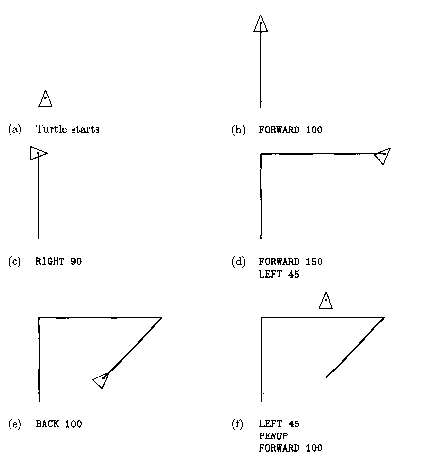
\includegraphics[scale=1]{fig1-1}
\caption{A sequence of turtle commands}
\end{center}
\end{figure}

In describing the effects of these operations, we say that \textsc{forward} and \textsc{back} change the turtle's {\em position} (the point on the plane where the turtle is located); \textsc{right} and \textsc{left} change the turtle's {\em heading} (the direction in which the turtle is facing). 

The turtle can leave a trace of the places it has been: The position-changing commands can cause lines to appear on the screen. This is controlled by the commands \textsc{penup} and \textsc{pendown}. When the pen is down, the turtle draws lines. Figure 1.1 illustrates how you can draw on the display screen by steering the turtle with \textsc{forward}, \textsc{back}, \textsc{right}, and \textsc{left}.

\subsection{Procedures}
Turtle geometry would be rather dull if it did not allow us to teach the
turtle new commands. But luckily all we have to do to teach the turtle a
new trick is to give it a list of commands it already knows. For example,
here's how to draw a square with sides 100 units long:
\begin{verbatim}
TO SQUARE
   FORWARD 100
   RIGHT 90
   FORWARD 100
   RIGHT 90
   FORWARD 100
   RIGHT 90
   FORWARD 100
\end{verbatim}
This is an example of a {\em procedure}. (Such definitions are also commonly referred to as programs or functions.) The first line of the procedure (the {\em title line}) specifies the procedure's name. We've chosen to name this procedure \textsc{square}, but we could have named it anything at all. The rest of the procedure (the body) specifies a list of instructions the turtle is to carry out in response to the \textsc{square} command. There are a few useful tricks for writing procedures. One of them is called {\em iteration}, meaning repetition --- doing something over and over. Here's a more concise way of telling the turtle to draw a square, using iteration:

\begin{verbatim}
TO SQUARE
   REPEAT 4
      FORWARD 100
      RIGHT 90
\end{verbatim}
This procedure will repeat the indented commands \textsc{forward} 100 and \textsc{right} 90 four times.

Another trick is to create a \textsc{square} procedure that takes an input for the size of the square. To do this, specify a name for the input in the title line of the procedure, and use the name in the procedure body:

\begin{verbatim}
TO SQUARE SIZE
   REPEAT 4
      FORWARD SIZE
      RIGHT 90
\end{verbatim}
Now, when you use the command, you must specify the value to be used for the 
input, so you say \textsc{square 100}, just like \textsc{forward 100}. 

The chunk \textsc{forward size}, \textsc{right 90}  might be useful in other 
contexts, which is a good reason to make it a procedure in its own right:


\begin{verbatim}
TO SQUAREPIECE SIZE
   FORWARD SIZE
   RIGHT 90
\end{verbatim}
Now we can rewrite \textsc{square} using \textsc{squarepiece} as

\begin{verbatim}
TO SQUARE SIZE
   REPEAT 4
   SQUAREPIECE SIZE
\end{verbatim}
Notice that the input to \textsc{square}, also called \textsc{size}, 
is passed in turn as an input to \textsc{squarepiece}. \textsc{squarepiece} 
can be used as a {\em subprocedure} in other places as well --- for example, in drawing 
a rectangle:

\begin{verbatim}
TO RECTANGLE SIDE1 SIDE2
   REPEAT 2
      SQUAREPIECE SIDE1
      SQUAREPIECE SIDE2
\end{verbatim}
To use the \textsc{rectangle} procedure you must specify its two inputs, for
example, \textsc{rectangle 100 50}.

When programs become more complex this kind of input notation
can be a bit hard to read, especially when there are procedures such as
\textsc{rectangle} that take more than one input. Sometimes it helps to use
parentheses and commas to separate inputs to procedures. For example,
the \textsc{rectangle} procedure can be written as

\begin{verbatim}
TO RECTANGLE (SIDE1, SIDE2)
   REPEAT 2
       SQUAREPIECE (SIDE1)
       SQUAREPIECE (SIDE2)
\end{verbatim}
If you like, you can regard this notation as a computer language that
has been designed to make it easy to interact with turtles. Appendix
A gives some of the details of this language. It should not be diflicult
to rewrite these procedures in any language that has access to the basic
turtle commands \textsc{forward}, \textsc{back}, \textsc{right}, \textsc{left}, \textsc{penup}, and \textsc{pendown}.


\begin{figure}
\begin{center}
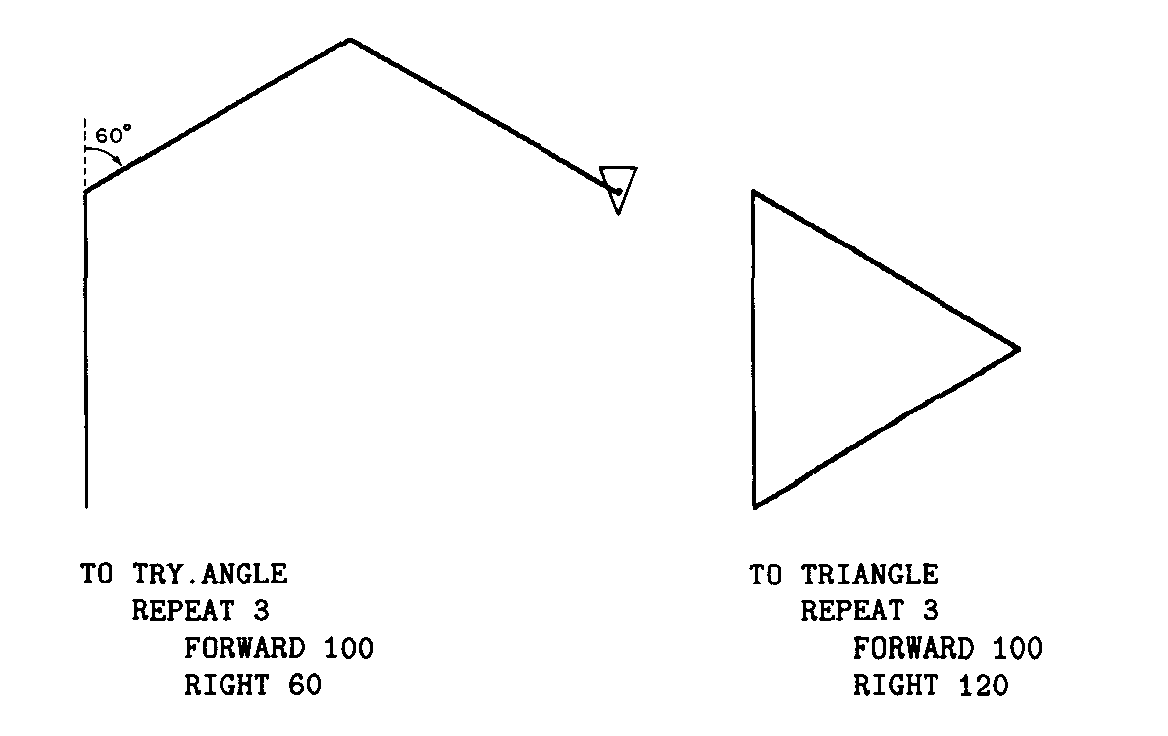
\includegraphics[scale=1]{fig1-2}
\caption{Attempt to draw a triangle}
\end{center}
\end{figure}

Appendix B gives some tips on how to implement these commands in
some of the more common computer languages, and includes sample
translations of turtle procedures.

\subsection{Drawing with the Turtle}
Let's draw a figure that doesn't use $90^{\circ}$ angles --- an equilateral triangle. Since the triangle has $60^{\circ}$ angles, a natural first guess at a triangle procedure is

\begin{verbatim}
TO TRY.ANGLE SIZE
   REPEAT 3
      FORWARD SIZE
      RIGHT 60
\end{verbatim}
But \textsc{try.angle} doesn't work, as shown in figure 1.2. In fact, running this ``triangle'' procedure draws half of a regular hexagon. The bug in the procedure is that, whereas we normally measure geometric figures by their interior angles, turtle turning corresponds to the exterior angle at the vertex. So if we want to draw a triangle we should have the turtle turn 120°. You might practice ``playing turtle'' on a few geometric figures until it becomes natural for you to think of measuring a vertex by how much the turtle must turn in drawing the vertex, rather than by the usual interior angle. Turtle angle has many advantages over interior angle, as you will see.

\begin{figure}
\begin{center}
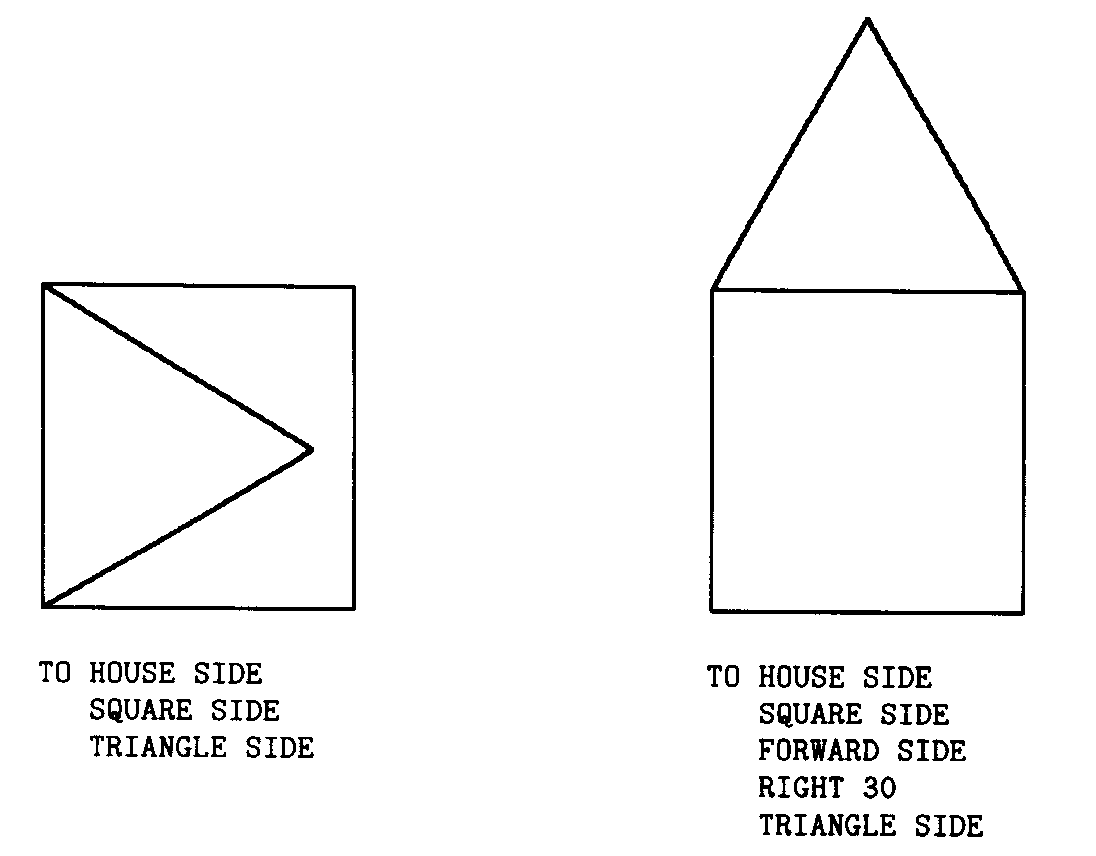
\includegraphics[scale=1]{fig1-3}
\caption{(a) Initial attempt to draw house fails (b) Interface steps are needed}
\end{center}
\end{figure}


Now that we have a triangle and a square, we can use them as building blocks in more complex drawings --- a house, for example. But Figure 1.3 shows that simply running \textsc{square} followed by \textsc{triangle} doesn't quite work. The reason is that after \textsc{square}, the turtle is at neither the correct position nor the correct heading to begin drawing the roof. To fix this bug, we must add steps to the procedure that will move and rotate the turtle before the \textsc{triangle} procedure is run. In terms of designing programs to draw things, these extra steps serve as an interface between the part of the program that draws the walls of the house (the \textsc{square} procedure) and the part that draws the roof (the \textsc{triangle} procedure).

\begin{figure}
\begin{center}
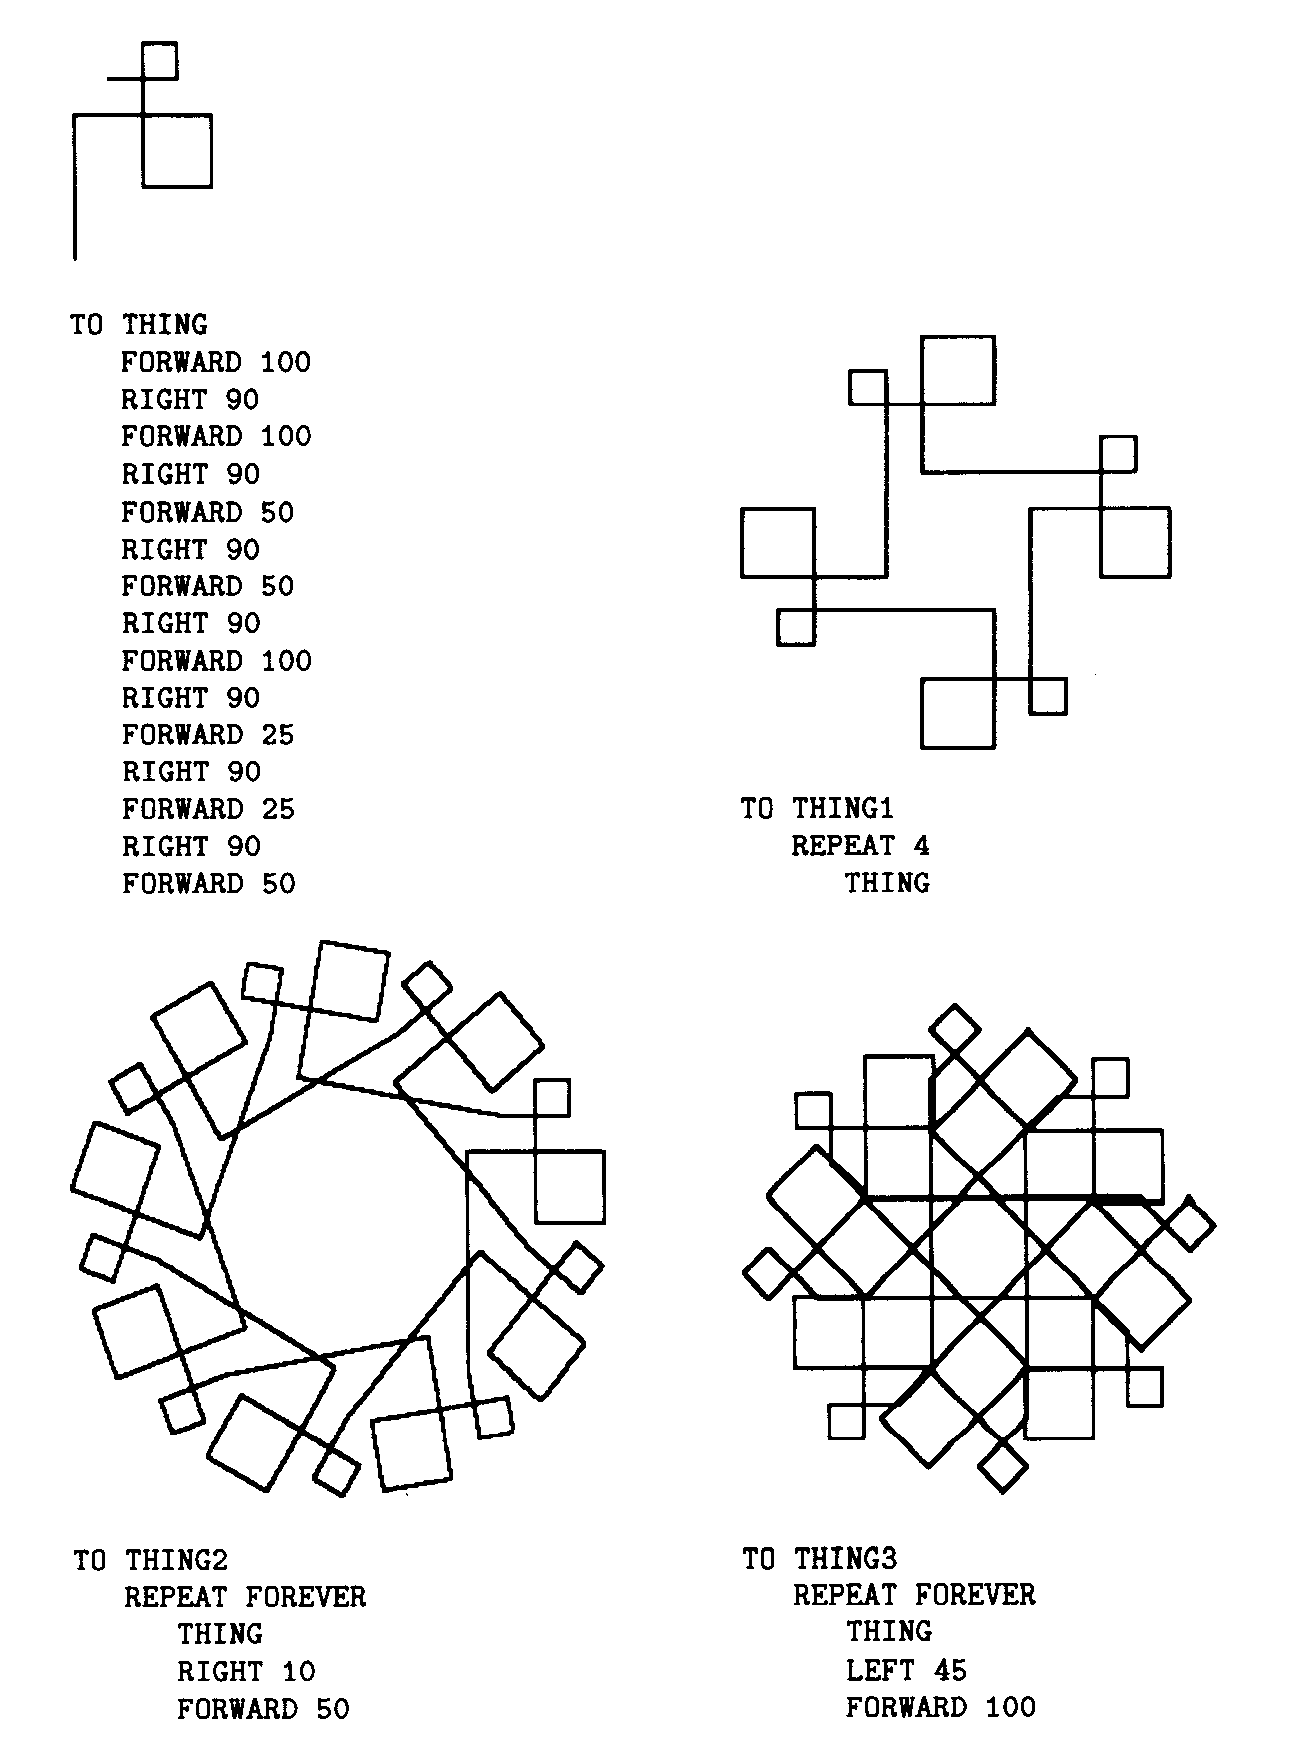
\includegraphics[scale=1]{fig1-4}
\caption{Designs made by rotating a simple doodle}
\end{center}
\end{figure}


In general, thinking of procedures as a number of main steps separated by interfaces is a useful strategy for planning complex drawings. Using procedures and subprocedures is also a good way to create abstract designs. Figure 1.4 shows how to create elaborate patterns by rotating a simple ``doodle''.

After all these straight line drawings, it is natural to ask whether the turtle can also draw curves --- circles, for example. One easy way to do this is to make the turtle go \textsc{forward} a little bit and then turn \textsc{right} a little bit, and repeat this over and over:

\begin{verbatim}
TO CIRCLE
   REPEAT FOREVER
      FORWARD 1
      RIGHT 1
\end{verbatim}
\begin{figure}
\begin{center}
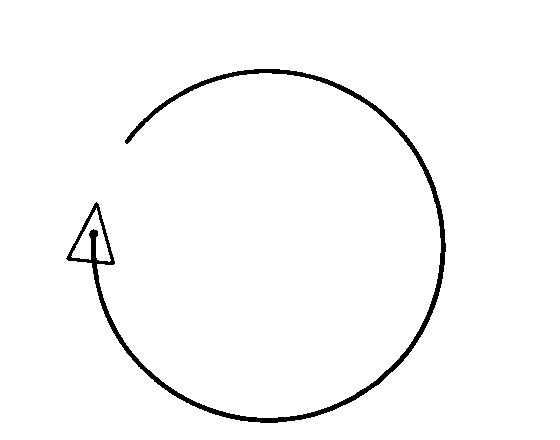
\includegraphics[scale=1]{fig1-5}
\caption{\textsc{forward} 1, \textsc{right} 1, repeated draws a circle}
\end{center}
\end{figure}

This draws a circular arc, as shown in figure 1.5. Since this program
goes on ``forever'' (until you press the stop button on your computer), it
is not very useful as a subprocedure in creating more complex iigures.
More useful would be a version of the \textsc{circle} procedure that would
draw the figure once and then stop. When we study the mathematics of
turtle geometry, we'll see that the turtle circle closes precisely when the
turtle has turned through $360^{\circ}$. So if we generate the circle in chunks
of \textsc{forward} 1, \textsc{right} 1, the circle will close after 
precisely 360 chunks:

\begin{verbatim}
TO CIRCLE
   REPEAT 360
      FORWARD 1
      RIGHT 1
\end{verbatim}
If we repeat the basic chunk fewer than 360 times, we get circular arcs.
For instance, 180 repetitions give a semicircle, and 60 repetitions give a
$60^{\circ}$ arc. The following procedures draw left and right arcs of \textsc{deg} degrees
on a circle of size \textsc{r}:

\begin{verbatim}
T0 ARCR R DEG
   REPEAT DEG
   FORWARD R
   RIGHT 1

TO ARCL R DEG
   REPEAT DEG
      FORWARD R
      LEFT 1
\end{verbatim}
(See figure 1.6 and exercise 3 for more on making drawings with arcs.)

The circle program above actually draws regular 360-gons, of course,
rather than ``real'' circles, but for the purpose of making drawings on
the display screen this difference is irrelevant. (See exercises 1 and 2.)

\subsection{Turtle Geometry versus Coordinate Geometry}

We can think of turtle commands as a way to draw geometric figures on
a computer display. But we can also regard them as a way to describe
figures. Let's compare turtle descriptions with a more familiar system
for representing geometric figures --- the Cartesian coordinate system, in
which points are specified by two numbers, the $x$ and $y$ coordinates relative to a pair of axes drawn in the plane. To put Cartesian coordinates
into our computer framework, imagine a ``Cartesian turtle'' whose moves
are directed by a command called \textsc{setxy}. \textsc{setxy} takes two numbers as
inputs. These numbers are interpreted as at and y coordinates, and the
turtle moves to the corresponding point. We could draw a rectangle with
\textsc{setxy} using

\begin{verbatim}
TO CARTESIAN.RECTANGLE (WIDTH, HEIGHT)
   SETXY (WIDTH, 0)
   SETXY (WIDTH, HEIGHT)
   SETXY (O, HEIGHT)
   SETXY (O, O)
\end{verbatim}

\begin{figure}
\begin{center}
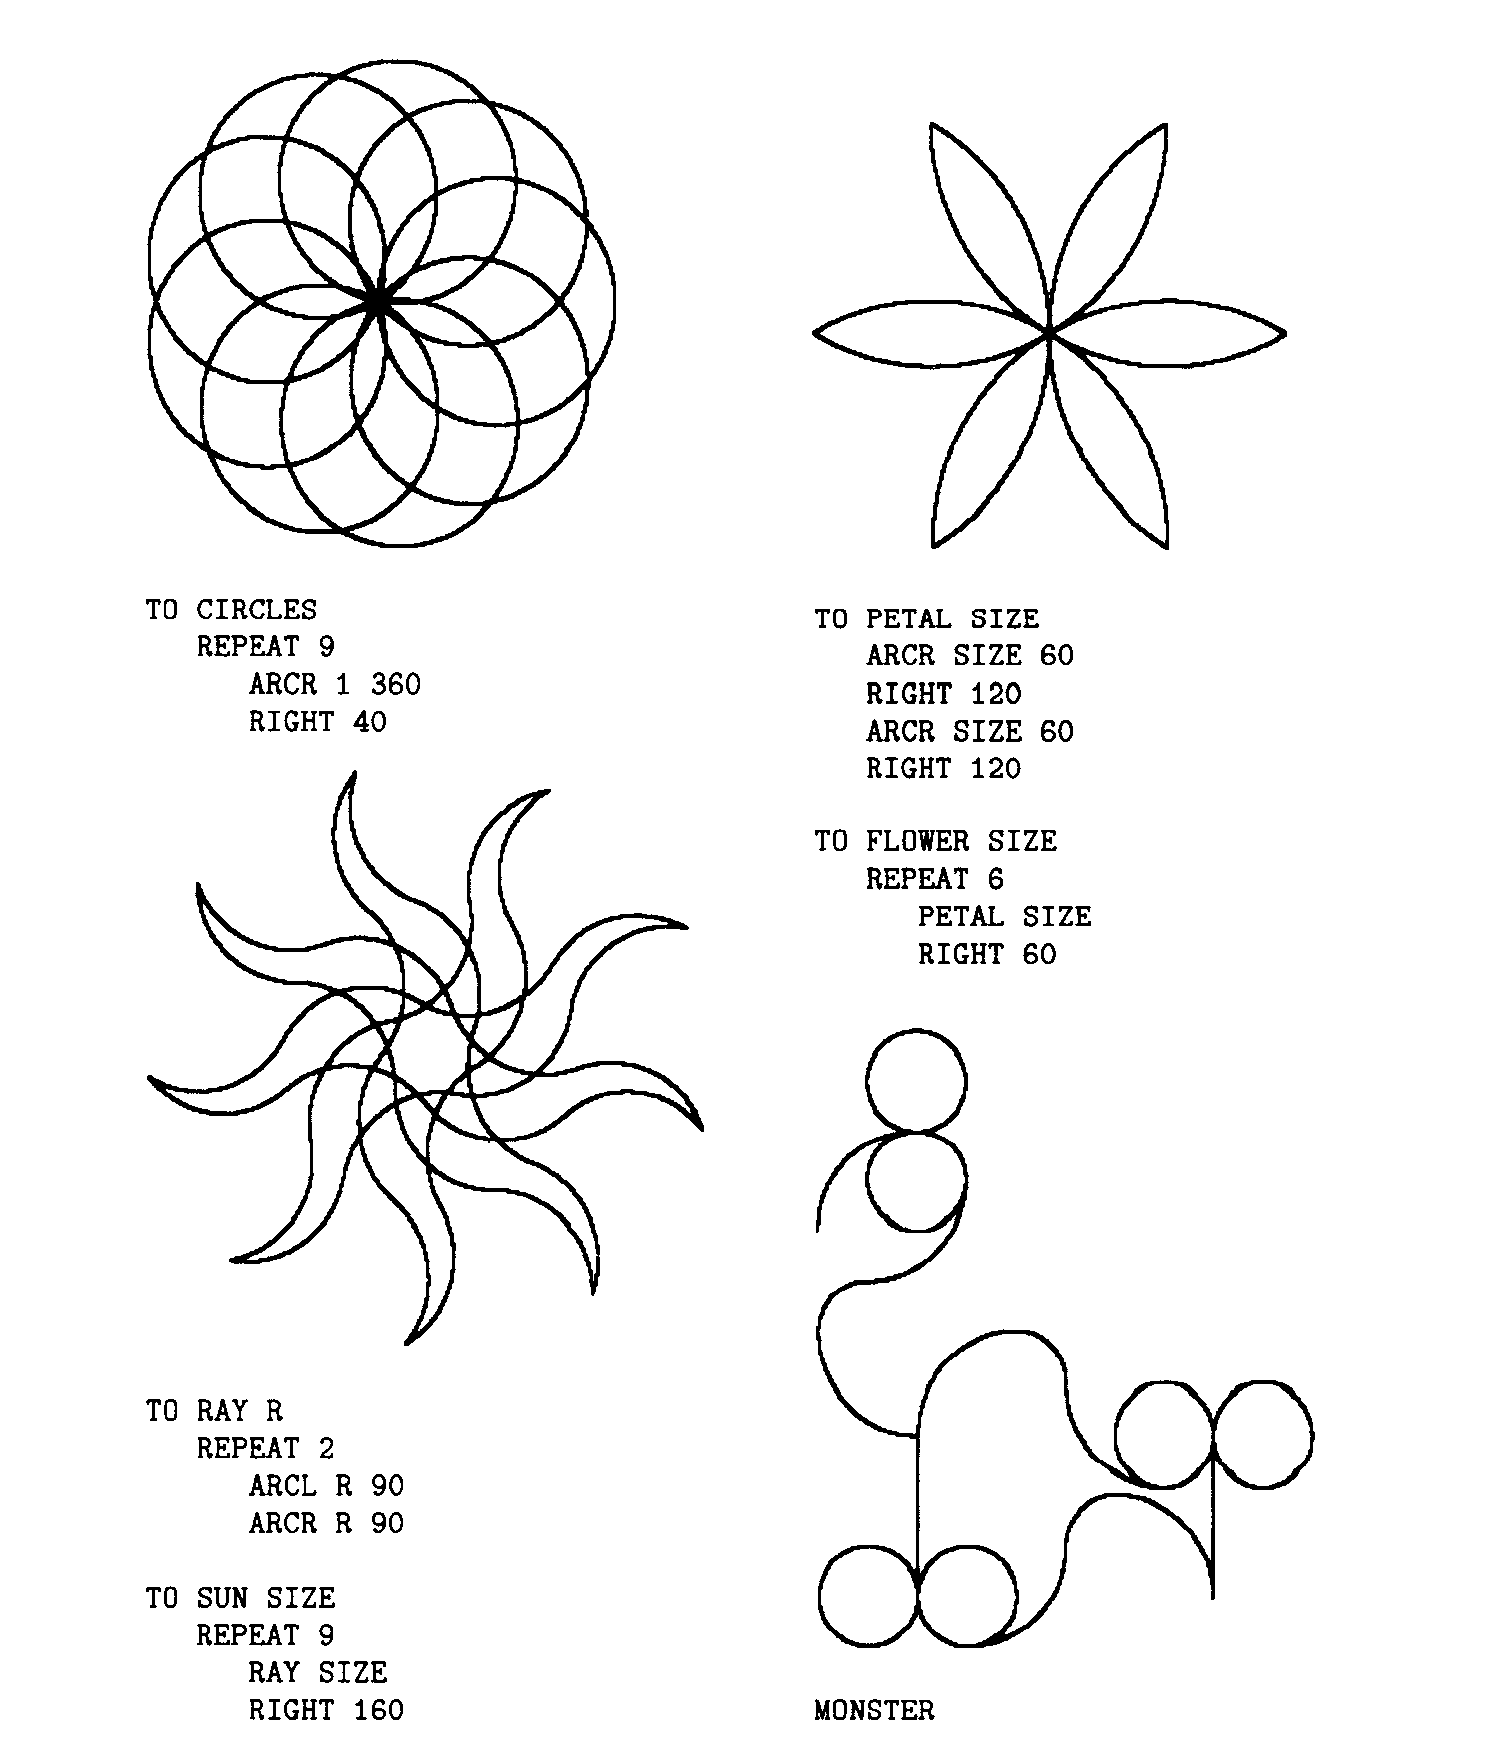
\includegraphics[scale=1]{fig1-6}
\caption{Some shapes that can be made using arcs}
\end{center}
\end{figure}

You are probably familiar with the uses of coordinates in geometry:
studying geometric figures via equations, plotting graphs of numerical
relationships, and so on. Indeed, Descartes' marriage of algebra and
geometry is one of the fundamental insights in the development of mathematics. Nevertheless, these kinds of coordinate systems --- Cartesian,
polar, or what have you --- are not the only ways to relate numbers to
geometry. The turtle \textsc{forward} and \textsc{right} commands give an alternative way of measuring figures in the plane, a way that complements the
coordinate viewpoint. The geometry of coordinates is called coordinate
geometry we shall refer to the geometry of \textsc{forward} and \textsc{right} as turtle
geometry. And even though we will be making use of coordinates later
on, let us begin by studying turtle geometry as a system in its own right.
Whereas studying coordinate geometry leads to graphs and algebraic
equations, turtle geometry will introduce some less familiar, but no less
important, mathematical ideas.

\subsubsection{Intrinsic versus Extrinsic}

One major difference between turtle geometry and coordinate geometry
rests on the notion of the {\em intrinsic} properties of geometric figures. An
intrinsic property is one which depends only on the figure in question,
not on the figure's relation to a frame of reference. The fact that a
rectangle has four equal angles is intrinsic to the rectangle. But the
fact that a particular rectangle has two vertical sides is {\em extrinsic}, for
an external reference frame is required to determine which direction is
``vertical.'' Turtles prefer intrinsic descriptions of figures. For example,
the turtle program to draw a rectangle can draw the rectangle in any
orientation (depending on the turtle's initial heading), but the program
\textsc{cartesian.rectangle} shown above would have to be modified if we
did not want the sides of the rectangle drawn parallel to the coordinate
axes, or one vertex at (0,0).

\begin{figure}
\begin{center}
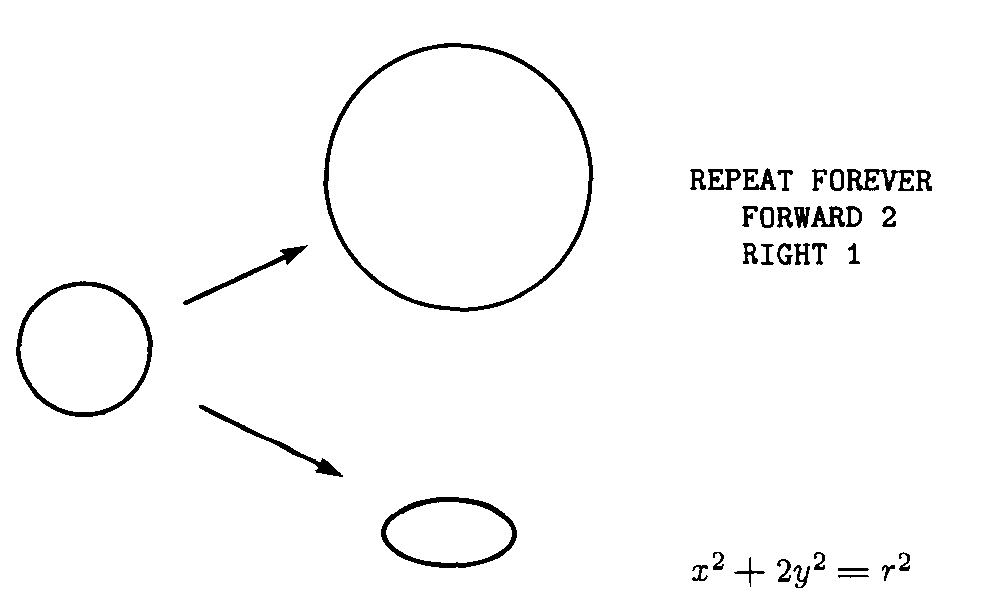
\includegraphics[scale=1]{fig1-7}
\caption{Modifying the turtle program still produces a circle. Modifying the equation gives an ellipse.}
\end{center}
\end{figure}

Another intrinsic property is illustrated by the turtle program for
drawing a circle: Go \textsc{forward} a little bit, turn \textsc{right} a little bit, and
repeat this over and over. Contrast this with the Cartesian coordinate
representation for a circle, $x^2 + y^2 = r^2$. The turtle representation
makes it evident that the curve is everywhere the same, since the process
that draws it does the same thing over and over. This property of the
circle, however, is not at all evident from the Cartesian representation.
Compare the modified program
\begin{verbatim}
TO CIRCLE
   REPEAT FOREVER
      FORWARD 2
      RIGHT 1
\end{verbatim}with the modified equation $x^2 + 2y^2 = r^2$. (See figure 1.7.) The drawing
produced by the modified program is still everywhere the same, that is, a
circle. In fact, it doesn't matter what inputs we use to \textsc{forward} or \textsc{right}
(as long as they are small). We still get a circle. The modified equation,
however, no longer describes a circle, but rather an ellipse whose sides
look different from its top and bottom. A turtle drawing an ellipse would
have to turn more per distance traveled to get around its ``pointy'' sides
than to get around its flatter top and bottom. This notion of ``how
pointy something is,'' expressed as the ratio of angle turned to distance
traveled, is the intrinsic quantity that mathematicians call {\em curvature}.
(See exercises 2 and 4.)

\subsubsection{Local versus Global}

The turtle representation of a circle is not only more intrinsic than the
Cartesian coordinate description. It is also more local; that is, it deals
with geometry a little piece at a time. The turtle can forget about the
rest of the plane when drawing a circle and deal only with the small part
of the plane that surrounds its current position. By contrast, $ x^2 + y^2 = r^2 $ relies on a large-scale, global coordinate system to deline its properties.
And defining a circle to be the set of points equidistant from some fixed
point is just as global as using $ x^2 + y^2 = r^2$. The turtle representation
does not need to make reference to that ``faraway'' special point, the
center. In later chapters we will see how the fact that the turtle does its
geometry by feeling a little locality of the world at a time allows turtle
geometry to extend easily out of the plane to curved surfaces.

\subsubsection{Procedures versus Equations} 

A final important difference between turtle geometry and coordinate
geometry is that turtle geometry characteristically describes geometric
objects in terms of procedures rather than in terms of equations. In 
formulating turtle-geometric descriptions we have access to an entire range
of procedural mechanisms (such as iteration) that are hard to capture in
the traditional algebraic formalism. Moreover, the procedural descriptions 
used in turtle geometry are readily modified in many ways. This
makes turtle geometry a fruitful arena for mathematical exploration.
Let's enter that arena now.

\subsection{Some Simple Turtle Programs}

If we were setting out to explore coordinate geometry we might begin
by examining the graphs of some simple algebraic equations. Our investigation of turtle geometry begins instead by examining the geometric
figures associated with simple procedures. Here's one of the simplest:
Go \textsc{forward} some fixed amount, turn \textsc{right} some fixed amount, 
and repeat this sequence over and over. This procedure is called \textsc{poly}.

\begin{verbatim}
TO POLY SIDE ANGLE
   REPEAT FOREVER
      FORWARD SIDE
      RIGHT ANGLE
\end{verbatim}
It draws shapes like those in figure 1.8.

\textsc{poly} is a generalization of some procedures we've already seen. Setting
the angle inputs equal to 90, 120, and 60, we get, respectively, squares,
equilateral triangles, and regular hexagons. Setting the angle input equal
to 1 gives a circle. Spend some time exploring \textsc{poly}, examining how the
figures vary as you change the inputs. Observe that rather than drawing
each figure only once, \textsc{poly} makes the turtle retrace the same path over
and over. (Later on we'll worry about how to make a version of \textsc{poly}
that draws a figure once and then stops.)

Another way to explore with \textsc{poly} is to modify not only the inputs,
but also the program; for example (see figure 1.9),

\begin{verbatim}
TO NEWPOLY SIDE ANGLE
   REPEAT FOREVER
      FORWARD SIDE
      RIGHT ANGLE
      FORWARD SIDE
      RIGHT (2 * ANGLE)
\end{verbatim}
(The symbol ``*'' denotes multiplication.) You should have no difficulty
inventing many variations along these lines, particularly if you use such
procedures as \textsc{square} and \textsc{triangle} as subprocedures to 
replace or supplement \textsc{forward} and \textsc{right}.

\begin{figure}
\begin{center}
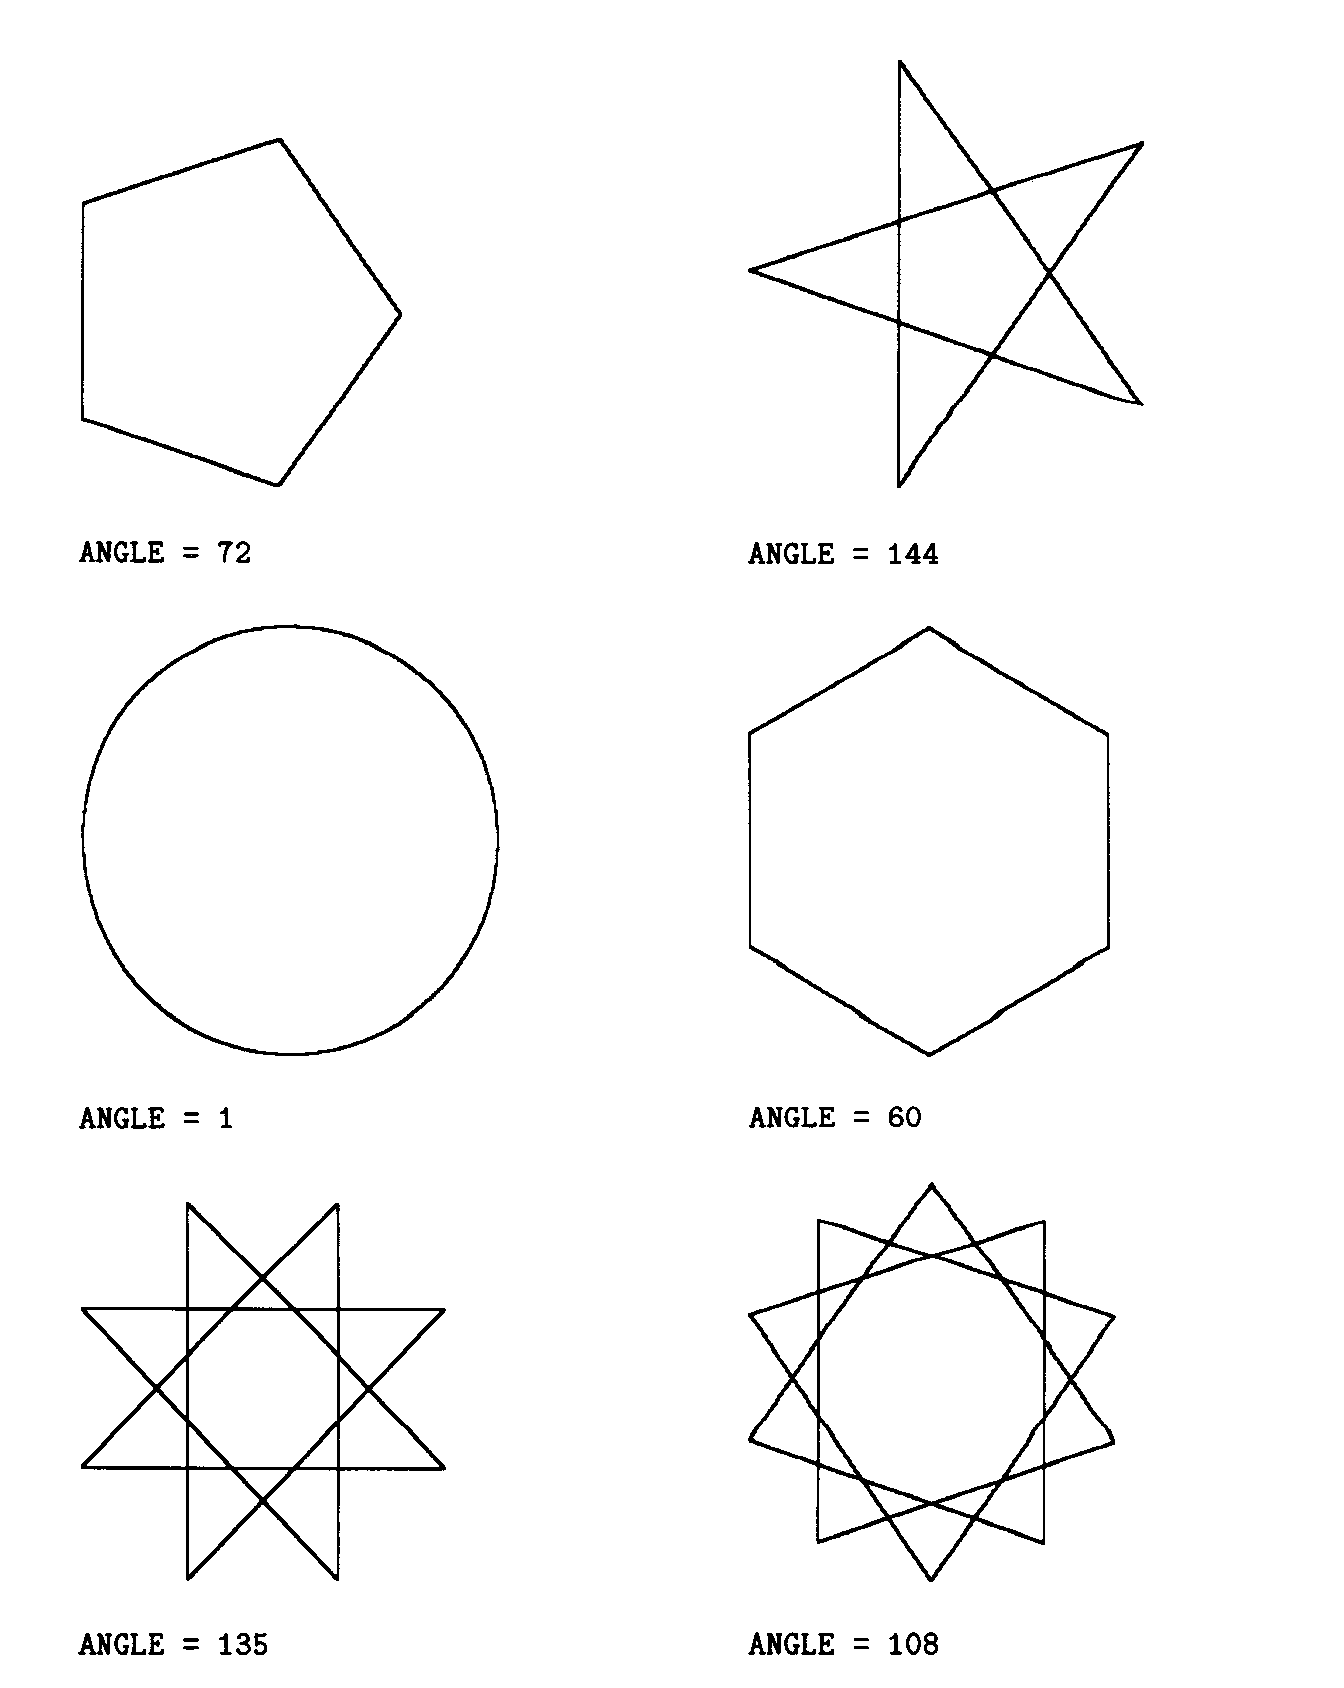
\includegraphics[scale=1]{fig1-8}
\caption{Shapes drawn by \textsc{poly}}
\end{center}
\end{figure}

\begin{figure}
\begin{center}
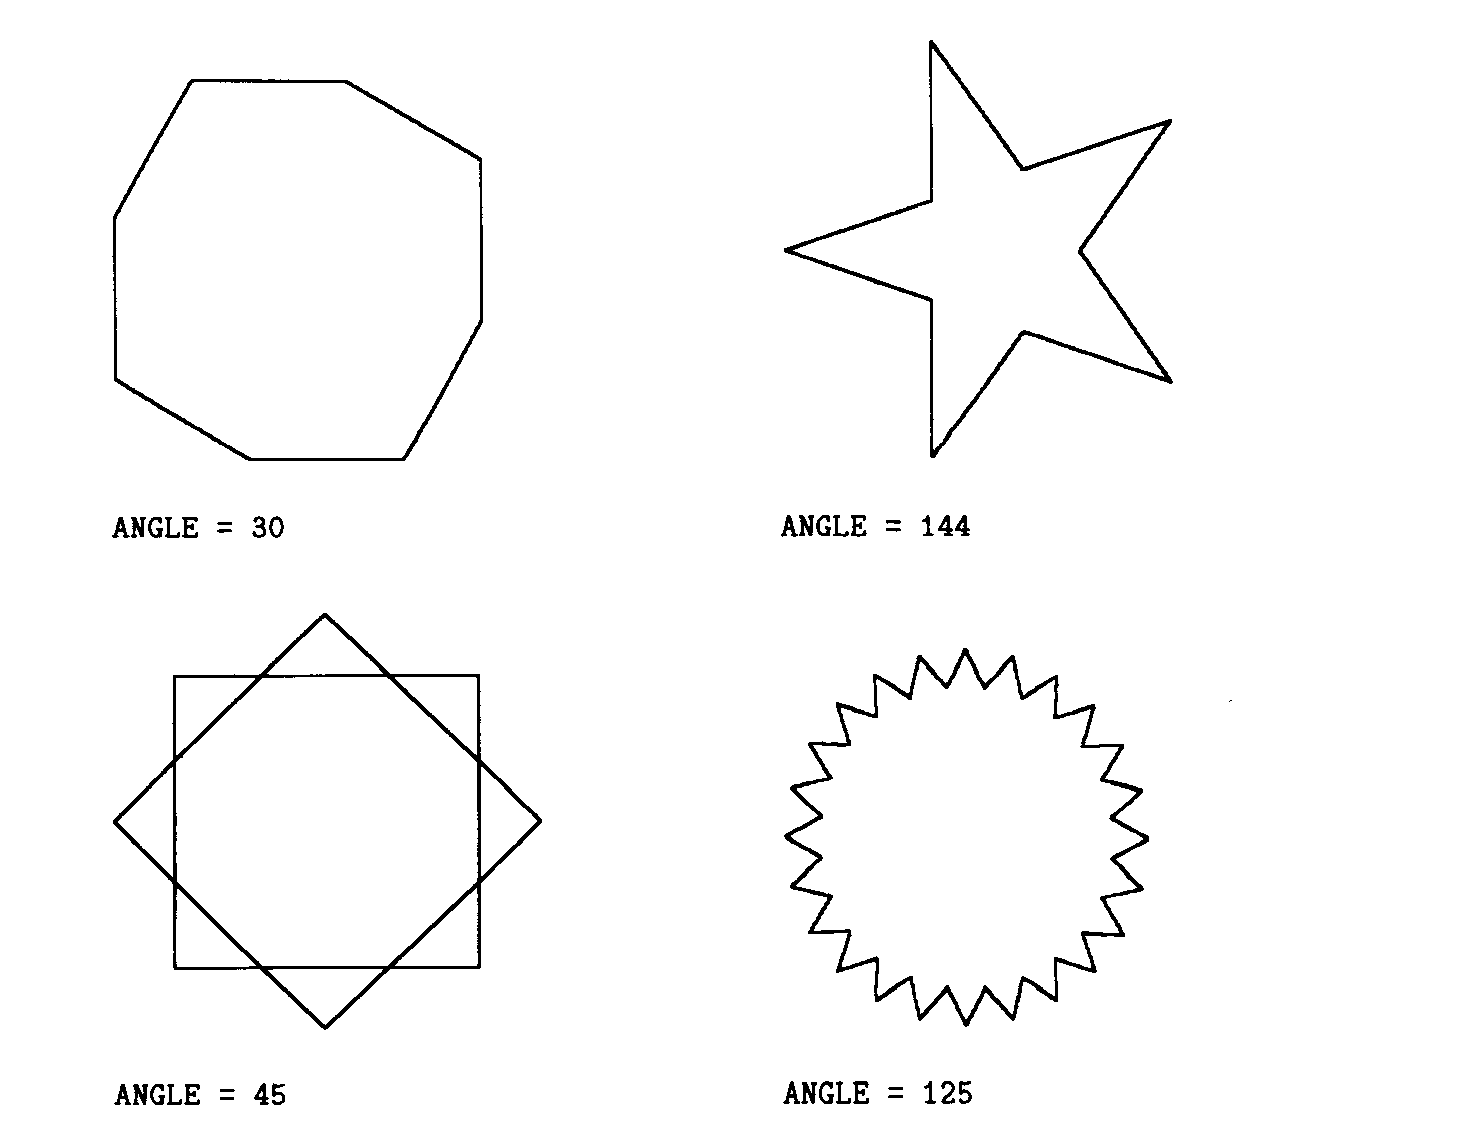
\includegraphics[scale=1]{fig1-9}
\caption{Shapes drawn by \textsc{newpoly}}
\end{center}
\end{figure}

\subsubsection{Recursion}

One particularly important way to make new procedures and vary old
ones is to employ a program control structure called {\em recursion}; that is,
to have a procedure use itself as a subprocedure, as in

\begin{verbatim}
TO POLY SIDE ANGLE
   FORWARD SIDE
   RIGHT ANGLE
   POLY SIDE ANGLE
\end{verbatim}
The final line keeps the process going over and over by including ``do \textsc{poly} again'' as part of the definition of \textsc{poly}.

\begin{figure}
\begin{center}
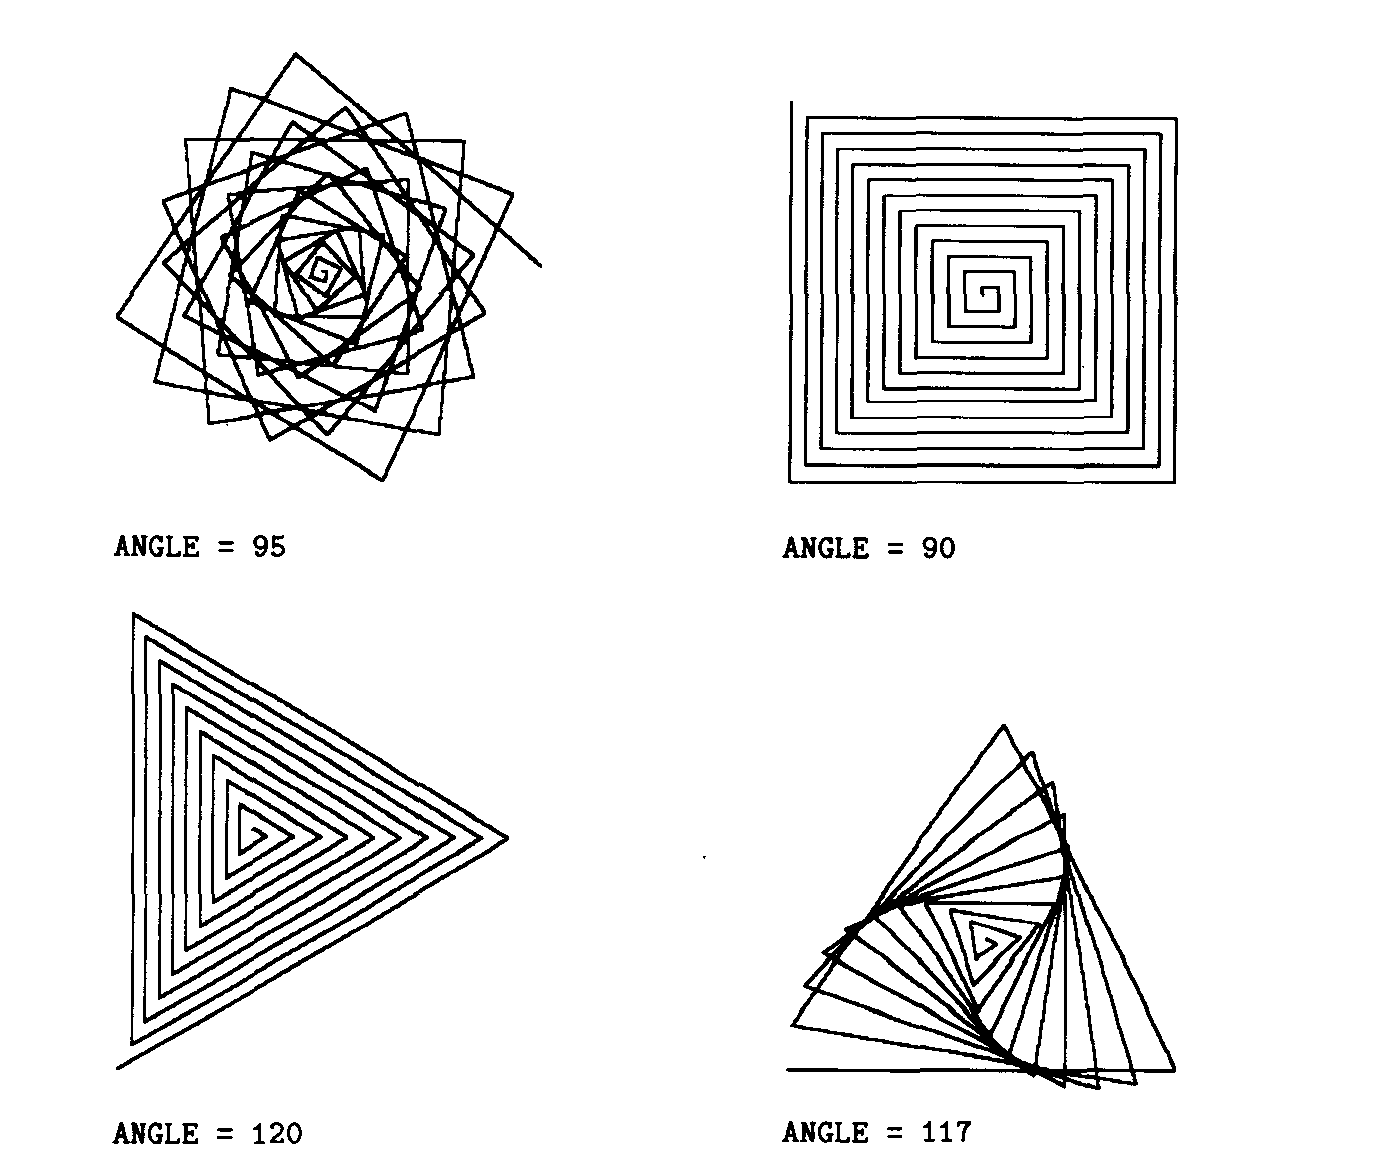
\includegraphics[scale=1]{fig1-10}
\caption{Shapes drawn by \textsc{polyspi}}
\end{center}
\end{figure}

One advantage of this slightly different way of representing \textsc{poly} is
that it suggests some further modifications to the basic program. For
instance, when it comes time to do \textsc{poly} again, call it with different
inputs: 

\begin{verbatim}
TO POLYSPI SIDE ANGLE
   FORWARD SIDE
   RIGHT ANGLE
   POLYSPI (SIDE + 1, ANGLE)
\end{verbatim}
Figure 1.10 shows some sample \textsc{polyspi} figures. Look carefully at how
the program generates these figures: Each time the turtle goes \textsc{forward}
it goes one unit farther than the previous time.

\begin{figure}
\begin{center}
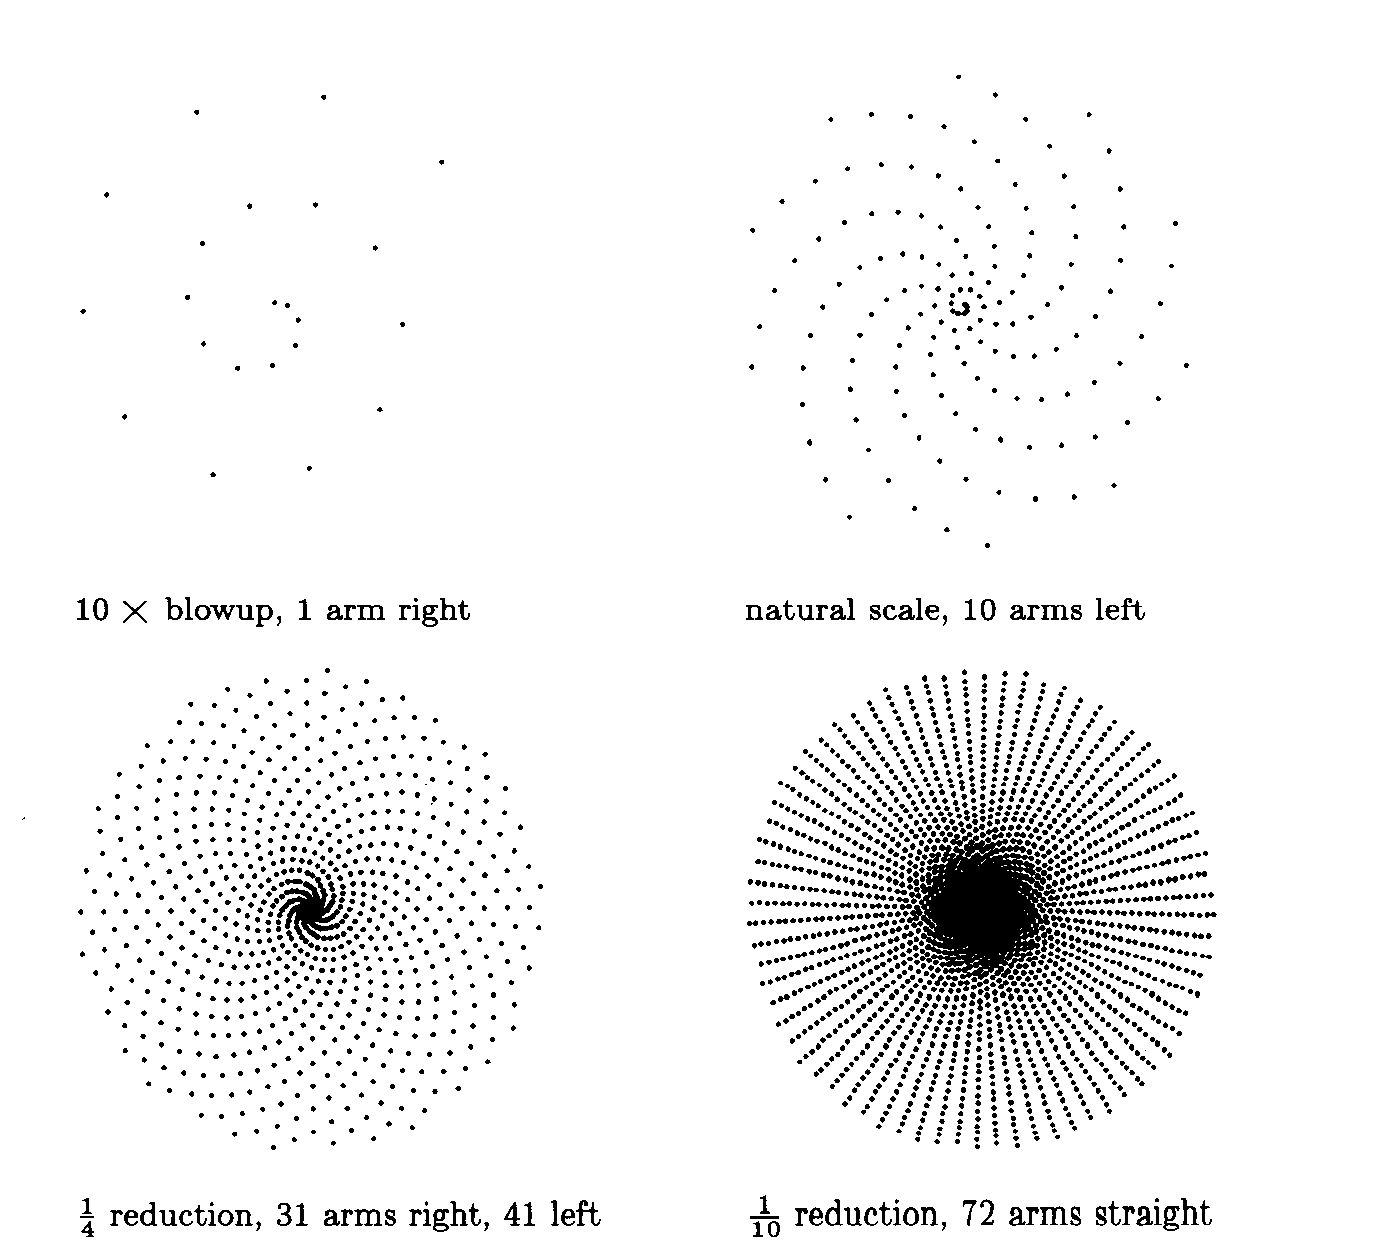
\includegraphics[scale=1]{fig1-11}
\caption{The vertices of a \textsc{polyspi}}
\end{center}
\end{figure}

A more general form of \textsc{polyspi} uses a third input (\textsc{inc}, for increment)
to allow us to vary how quickly the sides grow:

\begin{verbatim}
TO POLYSPI (SIDE, ANGLE, INC)
   FORWARD SIDE
   RIGHT ANGLE
   POLYSPI (SIDE + INC, ANGLE, INC)
\end{verbatim}
In addition to trying \textsc{polyspi} with various inputs, make up some of your
own variations. For example, subtract a bit from the side each time,
which will produce an inward spiral. Or double the side each time, or
divide it by two. Figure 1.11 illustrates a pattern made drawing only the
vertices of \textsc{polyspi}, shown at four scales of magnification (see 
exercise 13).  

\begin{figure}
\begin{center}
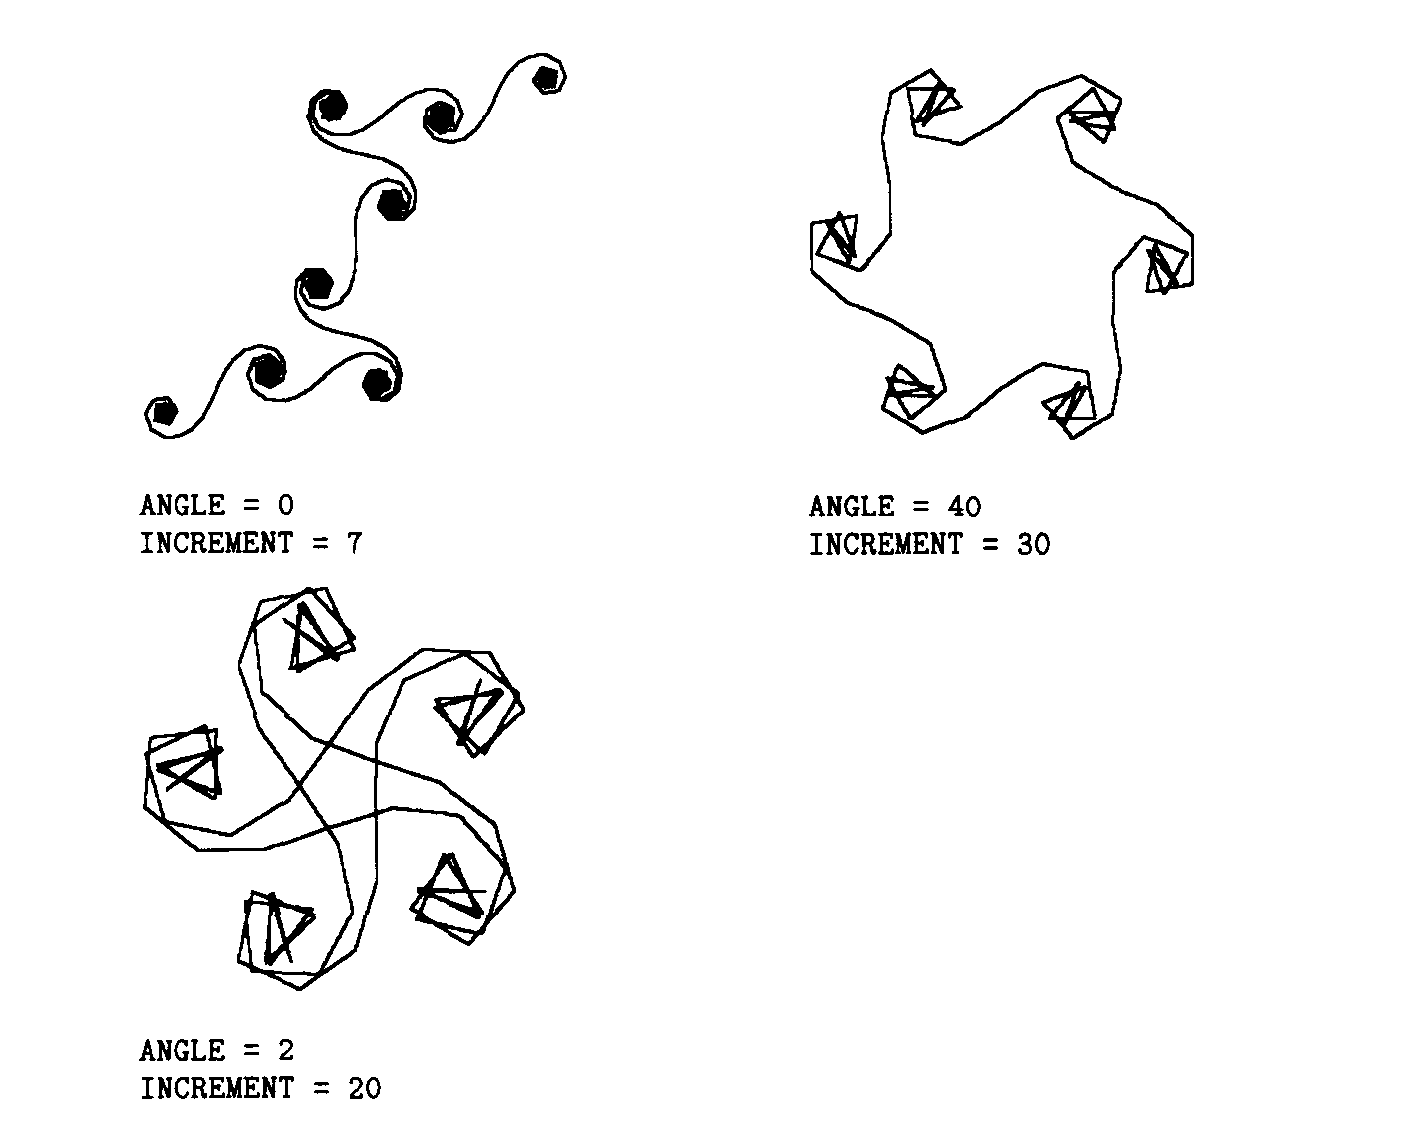
\includegraphics[scale=1]{fig1-12}
\caption{Examples of \textsc{inspi}}
\end{center}
\end{figure}

Another way to produce an inward spiral (curve of increasing curvature) is to increment the angle each time:

\begin{verbatim}
TO INSPI (SIDE, ANGLE, INC)
   FORWARD SIDE
   RIGHT ANGLE
   INSPI (SIDE, ANGLE + INC, INC)
\end{verbatim}
Run \textsc{inspi} and watch how it works. The turtle begins spiraling
inward as expected. But eventually the path begins to unwind as the
angle is incremented past $180^{\circ}$. Letting \textsc{inspi} continue, we 
find that it eventually produces a symmetrical closed figure which the turtle 
retraces over and over as shown in figure 1.12. You should find this surprising.
Why should this succession of \textsc{forward}s and \textsc{right}s bring the 
turtle back precisely to its starting point, so that it will then retrace its own path?
We will see in the next section that this closing phenomenon reflects the
elegant mathematics underlying turtle geometry.

\subsubsection{Exercises for Section \thesection}

\begin{enumerate}
\item We said in the text that when the inputs to the \textsc{poly} 
procedure are small, the resulting figure will be indistinguishable from a circle. Do
some experiments to see how large you can make the inputs and still
have the figure look like a circle. For example, is an angle of $20^{\circ}$ 
small enough to draw acceptable circles?

\item The sequence of figures \textsc{poly(2,2)}, \textsc{poly(1,1)}, \textsc{poly(.5, .5)}
all with the same curvature (turning divided by distance traveled), approaches ``in the limit'' a true mathematical circle. What is the radius
of the circle?  
\item $[P]$ Write a procedure that draws circular arcs. Inputs should specify
the number of degrees in the arc as well as the size of the circle. Can
you use the result of exercise 2 so that the size input is the radius of the
circle? [A]
\item Although the radius of a circle is not ``locally observable'' to a turtle
who is drawing the circle, that length is intimately related to a local
quantity called the ``radius of curvature,'' defined to be equal to $1 \div$
curvature, or equivalently, to distance divided by angle. What is the
relation between radius and radius of curvature for a \textsc{poly} with small
inputs as above? Do this when angle is measured in radians as well as
in degrees. [A]
\item $[P]$ Construct some drawings using squares, rectangles, triangles,
circles, and circular arc programs.
\item $[P]$ lnvent your own variations on the model of \textsc{polyspi} and \textsc{inspi}.
\item How many different 9-sided figures can \textsc{poly} draw (not counting
differences in size or orientation)? What angle inputs to \textsc{poly} produce
these figures? How about 10-sided figures? [A]
\item $[PD]$ A rectangle is a square with two different side lengths. More
generally, what happens to a \textsc{poly} that uses two different side lengths
as in the following program?

\begin{verbatim}
TO DOUBLEPOLY (SIDE1, SIDE2, ANGLE)
   REPEAT FOREVER
   POLYSTEP SIDE1 ANGLE
   POLYSTEP SIDE2 ANGLE
\end{verbatim}
In particular, how does the symmetry of \textsc{doublepoly} relate to that of
\textsc{poly} with the same \textsc{angle} input?  
\item $[D]$ Which encloses the larger area --- \textsc{poly(5, 5)} or \textsc{poly(6,6)}?
\item $[P]$ Find inputs to \textsc{inspi} that give a nonclosed figure. Can you give
a convincing argument that the figure is really nonclosed rather than,
say, a closed figure too big to fit on the display screen? [A]
\item $[P]$ If the display system you are using allows ``wraparound,'' you
can get some interesting effects by trying \textsc{poly}s with very large sides.
Explore these figures.  
\item There are three kinds of ``interchanges'' we can perform on turtle
programs: interchanging \textsc{right} and \textsc{left}, interchanging \textsc{forward} and
\textsc{back}, and (for programs that terminate) reversing the sequence of instructions. Describe in geometric terms the effect of each of these operations, both by itself and in combination with the others. Start with the
class of programs that close (return the turtle to its initial position and
heading). [HA]
\item $[P]$ The pattern made by the vertices of \textsc{polyspi} can be an interesting object of study. The dots seem to group into various ``arms,'' either
straight or curving left or right. To draw these patterns, you can use
the procedures

\begin{verbatim}
TO SPIDOT ANGLE
   SUBSPIDOT 0 ANGLE

TO SUBSPIDOT SIDE ANGLE
   FORWARD SIDE
   DOT
   RIGHT ANGLE
   SUBSPIDOT (SIDE + 1, ANGLE)

TO DOT
   PENDOWN
   FORWARD
   BACK 1
   PENUP
\end{verbatim}
For example, predict what you will see between \textsc{spidot 90}, which has
four arms, and \textsc{spidot 120}, which has three. Can you explain the
sequence of figures you actually do see? Figure 1.11 shows how the figure
drawn by the same \textsc{spidot} program seems to have different numbers
of spiral arms when viewed at different scales of magnification, which
can be accomplished by changing the increment to \textsc{side} in \textsc{subspidot}.
Study this phenomenon.  

\item $[P]$ Suppose we have a function called \textsc{random} that outputs a random
digit (0 through 9). Play around with the procedure

\begin{verbatim}
TO RANDPOLY SIDE ANGLE
   REPEAT FOREVER
      IF RANDOM = 0 THEN PENDOWN
         ELSE PENUP
      FORWARD SIDE
      RIGHT ANGLE
\end{verbatim}
Use this program as the basis for some psychology experiments. For
instance, what is the average number of sides that must be drawn before
people can recognize which \textsc{poly} it is?
\item $[D]$ Find some local and intrinsic way to describe an ellipse. Write
a program that makes the turtle draw ellipses, where the inputs specify
the size and eccentricity of the ellipse. [A]
\end{enumerate}


\section{POLYs and Other Closed Paths}

This section develops some general theorems about turtle programs by
studying one of the simplest of them, \textsc{poly}, which, when it closes,
exhibits clearly some properties shared by all closed paths, no matter
how complicated. Even when \textsc{poly} doesn't close, it can serve as a model
that clarifies symmetry and other important properties of a very general
class of programs. Careful and patient study of such a simple program
will be richly rewarded.

\subsection{The Closed-Path Theorem and the Simple-Closed-Path Theorem}

You have probably already noticed that \textsc{poly} with an angle input of
$360 / n$ draws a regular n-sided polygon. But it is not always true that
(number of sides) $\times$ (angle) $= 360$. If you try running \textsc{poly} with an angle
of 144 you will see that it draws a five-pointed star, and $5 \times 144 = 720$,
not 360. Noticing that 720 is exactly twice 360 might lead us to guess
the following formula:
$$\text{(number of sides)} \times \text{(angle)} = 360 \times \text{(an integer)}$$
It's not hard to see why this formula is true. The number of sides
times the angle is precisely the {\em total turning} done by the turtle in
walking once around the figure --- the net change in heading. If the
path is to close legitimately, and not just cross itself, then the turtle
must end its trip with the same heading it started out with. Thus,
the total turning must be some multiple of $360^{\circ}$.

Total turning is the central concept here. It certainly need not be
restricted to \textsc{poly}. One can imagine any turtle program keeping a
running count of its turning, adding in \textsc{right}s and subtracting \textsc{left}s.
Because only \textsc{right}s and \textsc{left}s change heading, this total turning is
always exactly the total change in heading. In particular, if the path is a
closed path (one which restores the turtle's initial position and heading),
we can be confident that the net turning ($=$ change of heading) is a
multiple of $360^{\circ}$. This gives us our first turtle-geometric theorem:

\vspace{0.5cm}

\noindent \textbf{Closed-Path Theorem} The total turning along any closed path is an
integer multiple of $360^{\circ}$.

\vspace{0.5cm}

Total turning is an intrinsic property of a path. It does not depend on
where the path starts, or how it is oriented with respect to ``vertical.''
The total turning of a closed path is frequently summarized simply by
the particular integer that multiplies 360. That integer is called the
{\em rotation number} of the path. As an exercise, follow the turtle around
the sample paths in figure 1.13 and compute the rotation numbers.

Does your experience with \textsc{poly} suggest an improvement to the closed-path 
theorem? A little experimentation should convince you that there
are two essentially different classes of \textsc{poly} paths: simple polygons (such
as squares, triangles, and hexagons); and star polygons (such as five-pointed stars), which are characterized by the fact that the paths cross
themselves. The simple polygons always appear to have total turning
equal to $+360^{\circ}$ or $-360^{\circ}$, depending upon the direction in which the
turtle traverses the path. The star polygons, however, always have total
turning different from $\pm 360^{\circ}$.

One wonders if this experimental correlation has general significance.
It is not hard to prove its validity for \textsc{poly}s (see exercise 11 below). But
the more important conjecture involves generalizing from \textsc{poly}s to any
{\em simple closed path} (a closed path that does not cross itself):

\vspace{0.5cm}

\noindent \textbf{Simple-Closed-Path Theorem} The total turning in a simple closed path
is $360^{\circ}$ (to the right or to the left). That is to say, the rotation number
of any simple closed path is $\pm 1$.

\vspace{0.5cm}

\begin{figure}
\begin{center}
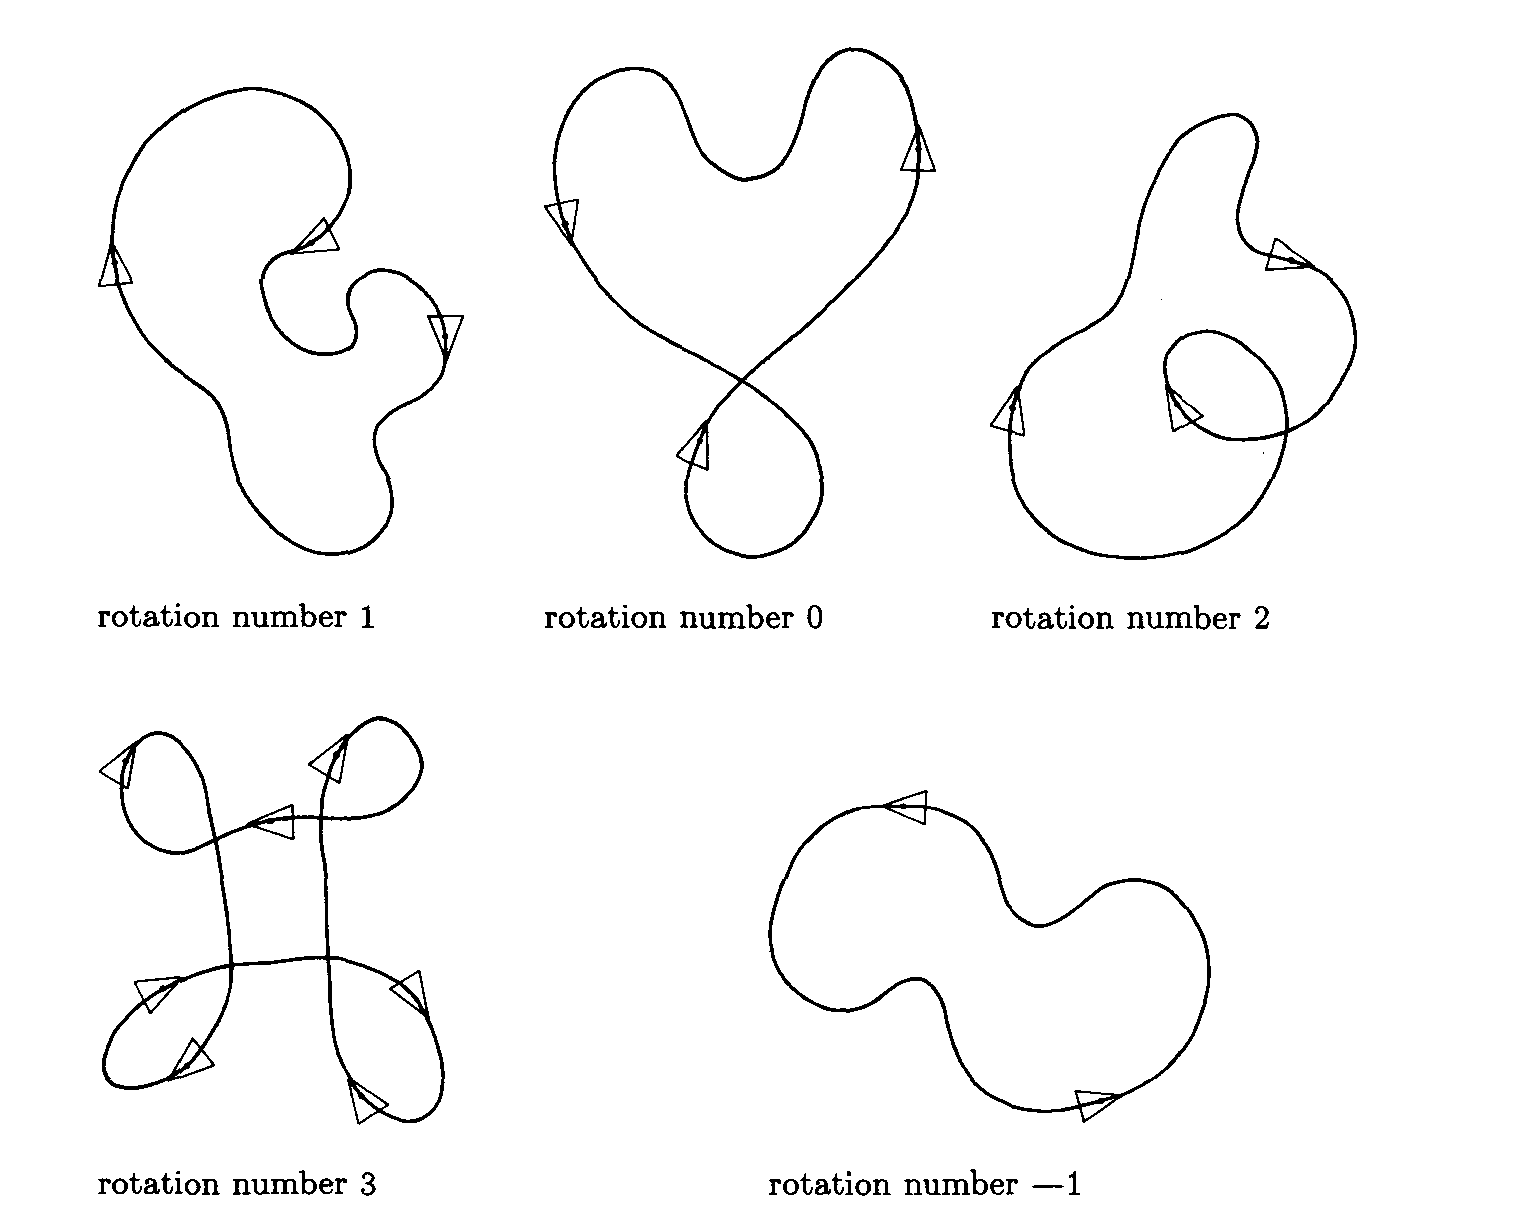
\includegraphics[scale=1]{fig1-13}
\caption{Rotation numbers of closed paths.}
\end{center}
\end{figure}

Take a look at some examples of simple closed paths to convince
yourself of the plausibility of this theorem, which is difficult to prove
rigorously. We will return to it later, in chapter 4. For now you should
note that this theorem says that there is a relation between two very
different aspects of a closed path --- the turning and the crossing points.
That makes it considerably less obvious than the closed-path theorem,
but also much more powerful. We give one example of the power here
and several more in the exercises.

The simple-closed-path theorem says that the sum of the exterior
angles of any simple polygon is $360^{\circ}$. For triangles, we can rewrite this
in terms of the three interior angles $A$, $B$, and $C$ to get
$$(180 - A) + (180 - B) + (180 - C) = 360$$
\noindent and thus
$$(A + B + C) = \text{the sum of interior angles} = 3 \times 180 - 360 = 180.$$

So, as a corollary of the simple-closed-path theorem, we have derived the
familiar result that the interior angles of a triangle must sum to $180^{\circ}$.

(Exercises 6-9 detail some other applications of the simple-closed-path
theorem.)

\subsection{The POLY Closing Theorem}

The \textsc{poly} procedures we've written so far, iterative and recursive, have
one fault: They neverstop. That makes it generally impossible to
use them as subprocedures in more complicated programs. Moreover,
the ``inefficiency'' of a drawing program that doesn't know when it is
done may simply offend one's sensibilities. The problem of making a
\textsc{poly} program that stops is a mathematical one with two fundamentally
different approaches.

The global approach is as follows: Sit back and look ahead. Given an
\textsc{angle} input, compute how many times the turtle must run the basic
\textsc{poly} step, \textsc{forward side}, \textsc{right angle}, before the path closes and
starts again. Then you need only repeat the \textsc{poly} step that many times.
The local approach revolves around questions like the following: How can
the turtle know, as it is walking along, when it is done? What clue can
the turtle be watching for? We will take the second approach here, as it
turns out to be simpler. The Hrst approach, however, is mathematically
rich and is pursued in section 1.4.

Consider: How could a turtle, while walking along drawing a \textsc{poly},
know when the figure has been completed? (A computer turtle cannot
see the lines it is drawing.) Thinking locally, the turtle knows only
two things, position and heading. Neither of these is truly local, for to
measure them usually involves a coordinate system. But the one locally
computable quantity we know about --- total turning --- can do the trick.
The closed-path theorem says that if the path closes, then total turning
must be a multiple of $360^{\circ}$. How about the converse: If the total turning
reaches a multiple of $360^{\circ}$, will the path be closed? This is not true for
turtle paths in general, but it is true for \textsc{poly}:

\vspace{0.5cm}

\noindent \textbf{POLY Closing Theorem} A path drawn by the \textsc{poly} procedure will close
precisely when the total turning reaches a multiple of $360^{\circ}$.

\vspace{0.5cm}

There is one bug in this theorem, one exceptional case: If the angle of
the \textsc{poly} is equal to 0 then the turtle just walks off along a straight
line. The path never closes, even though at every point the total
turning is 0, a perfectly good multiple of 360. But this exceptional case,
\textsc{forward side}, \textsc{right 0}, is transparent enough so that we can just leave
it out of consideration in most instances. Any multiple of $360^{\circ}$ will, of
course, have the same effect as a turn of 0.

\begin{figure}
\begin{center}
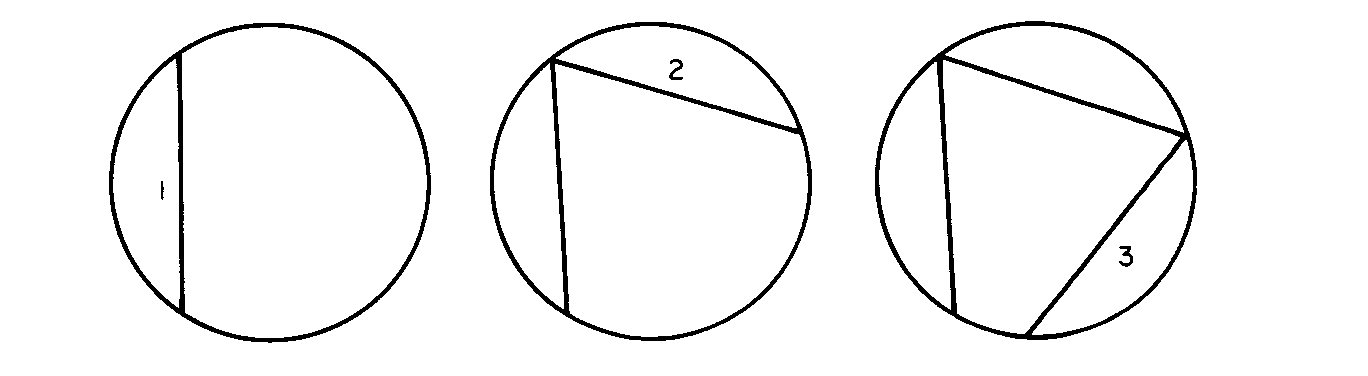
\includegraphics[scale=1]{fig1-14}
\caption{\textsc{poly} lays down a sequence of equal chords.}
\end{center}
\end{figure}

We'll outline two different proofs of the \textsc{poly} closing theorem.

\textbf{Sketch of Proof 1} Have you noticed the important fact that the vertices
of \textsc{poly} lie on a circle? (Everything about \textsc{poly} seems to be circular!) We leave the proof of this geometric fact to you in exercise 2. Using this fact, one can redescribe \textsc{poly} as the sequential laying down of fixed-length chords on a fixed circle as shown in figure 1.14. The point is that
there is only one chord of the required length that can be produced by
the turtle starting at any given heading. (Actually there are two, but
one of them has the wrong sense --- the turtle would turn off the circle
after traversing the chord.) Thus, whenever the turtle returns to its
initial heading (total turning = any multiple of $360^{\circ}$) it will be about to
retrace the first chord and so should stop. Notice how this proof breaks
down for the exceptional case \textsc{forward side}, \textsc{right 0}. The turtle must
do some turning or else the vertices will lie on a straight line rather than
on a circle.

An alternative proof is inspired less by geometry and more by ideas
from the theory of computation. It proceeds as follows.

\textbf{Sketch of Proof 2} Assume that we have a turtle following a \textsc{poly} procedure, and that at some time the turtle returns to its initial heading
(heading change = a multiple of $360^{\circ}$) but not to its initial position. We
will show that this assumption leads to a contradiction. (The trick of
the proof is to show that the turtle must walk off to infinity in some

\begin{figure}
\begin{center}
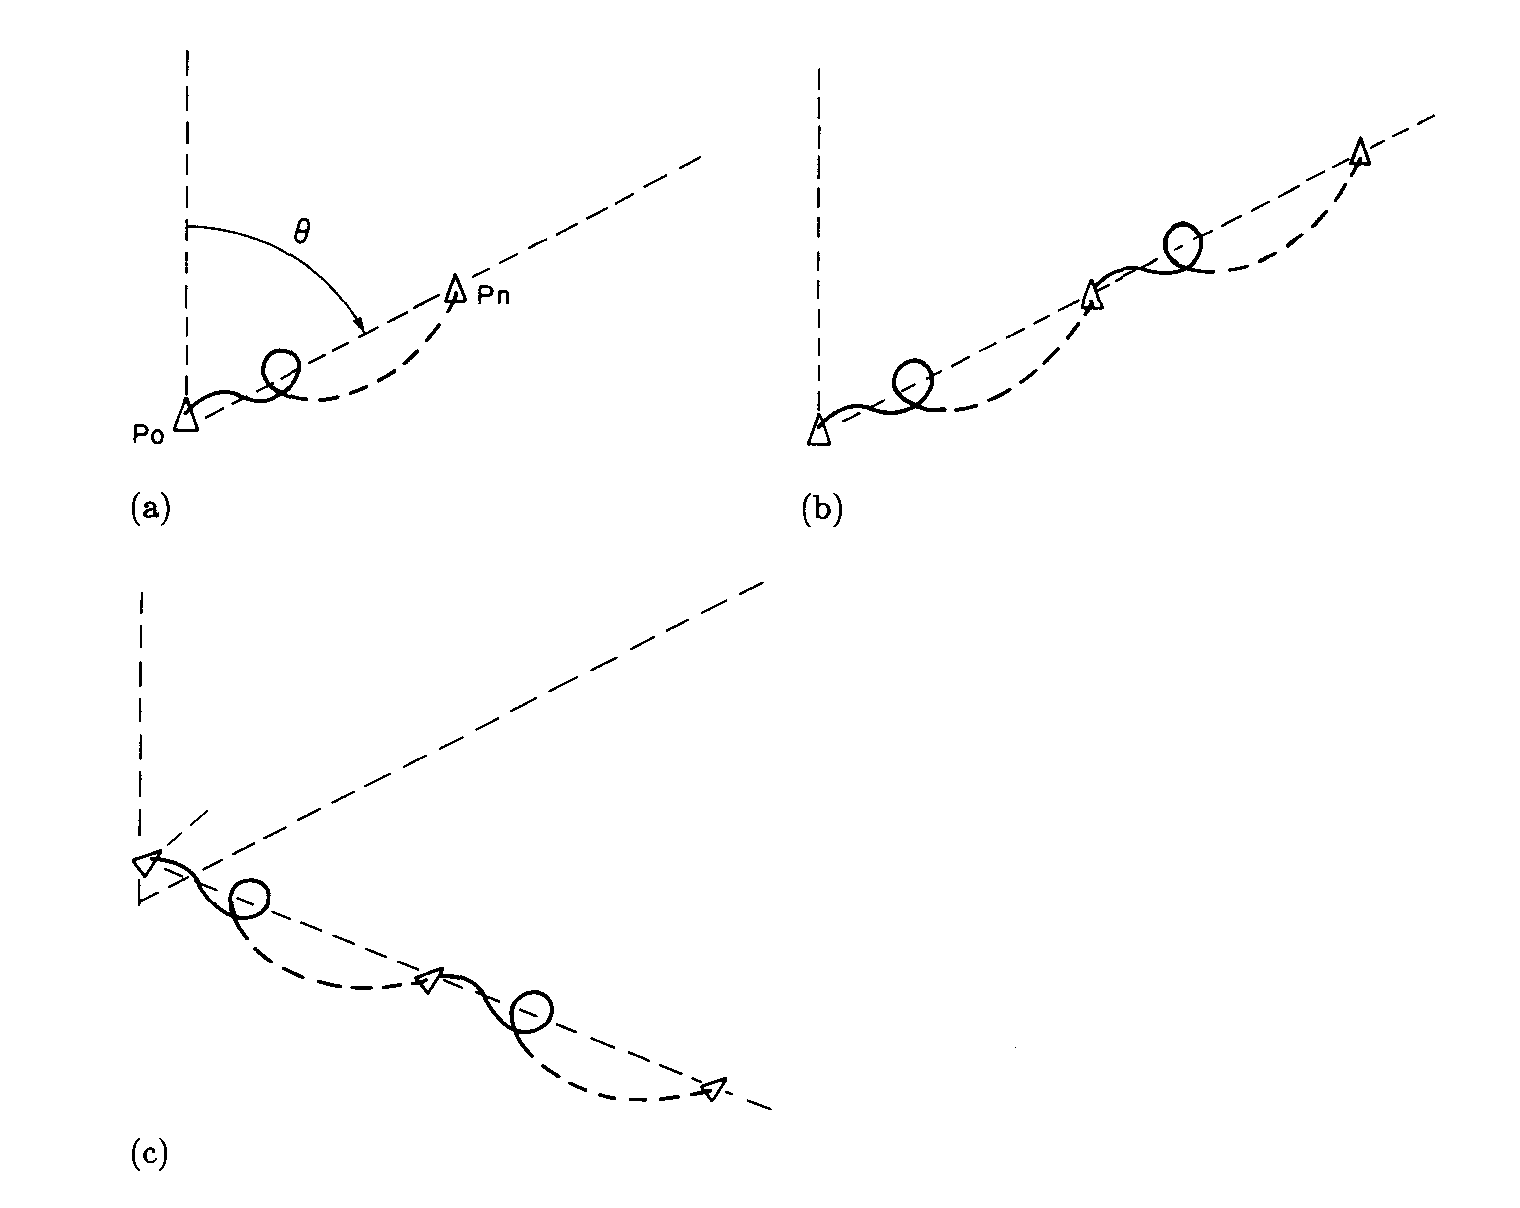
\includegraphics[scale=1]{fig1-15}
\caption{The \textsc{poly} closing theorem. (a) Suppose the turtle returns to his initial heading, but not his initial position. (b) $n$ more steps must do the same thing again. (c) From a new heading (after one \textsc{poly} step), chunks of $n$ steps carry the turtle away on a new line.}
\end{center}
\end{figure}

direction. Then, by regrouping the sequence of commands, we'll show
that the turtle runs off to iniinity in a different direction.)

\indent
By assumption, the turtle returns to its initial heading after some
number (say, $n$) repetitions of the \textsc{poly} step. (Notice that $n$ cannot
be 1 if we neglect the exceptional case \textsc{angle} = 0.) Draw a dotted
line connecting the turtle's initial position $p_0$ to its position $p_n$ after $n$
repetitions. This line makes some angle $\theta$ with the turtle's initial heading
(figure 1.15a).

Now let the turtle continue for $n$ more repetitions of the \textsc{poly} step.
Since the turtle starts out from $p_n$ with the same heading it had when
it started at $p_0$, the effect of n more \textsc{poly} steps will be to do the same
thing again, moving the turtle farther out along the same line, and again
bring it back to the initial heading (figure 1.15b). Continuing with $n$
more repetitions, and $n$ more, and so on, we see that the turtle must
run off infinitely far in the direction of the dotted line. Moreover, at no
point can the turtle's path stray very far from the line, since the turtle
must get back to it at the end of every $n$ \textsc{poly} steps.
Now let's return the turtle to the initial state and run the \textsc{poly} step
for one iteration. We will now see the turtle at a new position $p_1$ with a
different heading. lf we continue with $n$ repetitions from here, the turtle
will end up on a new dotted line that lies at angle $\theta$ to this new heading.
(Figure 1.15c).

But the problem is obvious now. Running another sequence of $n$,
then another and another, forces the turtle off infinitely far along this
new line. But the turtle cannot remain close to both dotted lines as it
marches off to infinity. This contradiction means that our assumption
that the turtle does not come back to the initial position must have been
wrong. This completes the proof.

This second proof demonstrates an important computational strategy:
Divide a process into meaningful chunks (for example, the parts of
the \textsc{poly} between equal headings), then pay close attention to the net
action of the chunks. Structuring a complex program as a group of
subprocedures illustrates the same strategy.

Here finally is our \textsc{poly} with stop rule:

\begin{verbatim}
TO POLYSTOP SIDE ANGLE
   TURN <- O
   REPEAT
      FORWARD SIDE
      RIGHT ANGLE
      TURN <- (TURN + ANGLE)
   UNTIL REMAINDER (TURN, 360) = 0
\end{verbatim}
Note the use of the new symbol $\leftarrow$, which means ``assign to the variable
on the left the value given on the right.'' The procedure \textsc{remainder} is
a function that computes the value of its first input modulo its second
input. The program also makes use of the iteration construct ``\textsc{repeat . . . until} (some condition)'', which keeps repeating the indented portion
until the condition is true (and always does the indented part at least
once).

\begin{figure}
\begin{center}
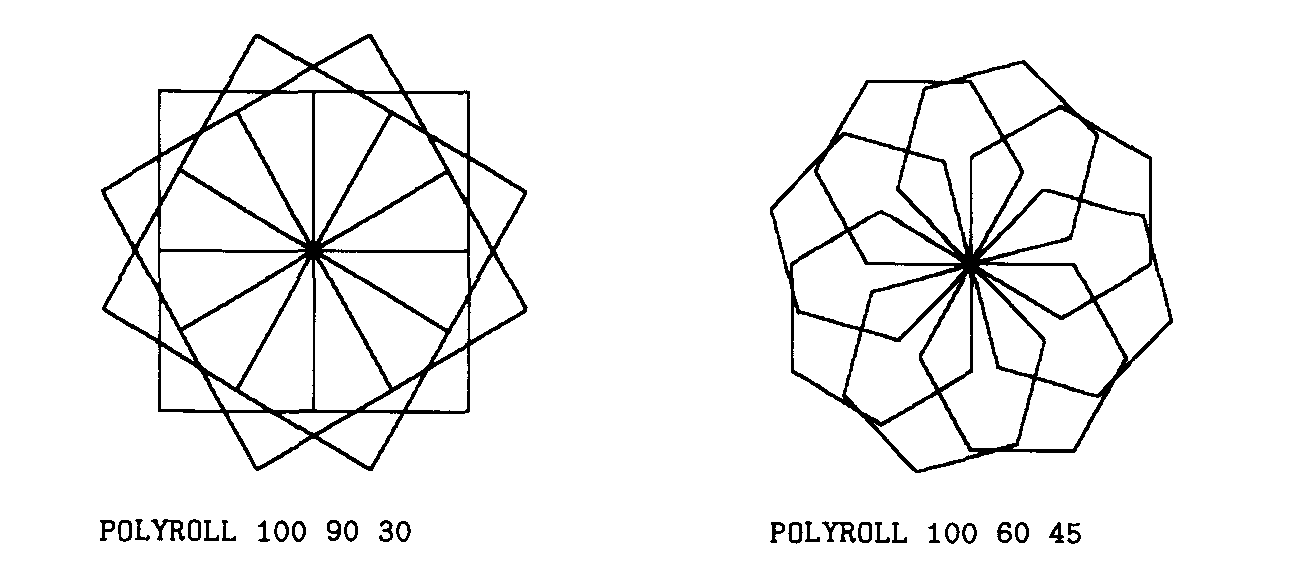
\includegraphics[scale=1]{fig1-16}
\caption{Examples of \textsc{polyroll}.}
\end{center}
\end{figure}

This program allows us to use \textsc{poly}s as building blocks in more complex figures; for example (see figure 1.16),

\begin{verbatim}
TO POLYROLL SIDE ANGLE1 ANGLE2 I
   REPEAT FOREVER
      POLYSTOP SIDE ANGLE1
      RIGHT ANGLE2
\end{verbatim}
\subsubsection{Exercises for Section \thesection}

\begin{enumerate}
\item The simple-closed-path theorem has a serious bug as it stands. It purports to give the precise multiple of 360 that describes the total turning
for a set of paths. Unfortunately, one can insert a step, \textsc{right 360},
that does not change the path at all, yet changes the multiple of 360
given by total turning. These gratuitous 360s must be pruned from
the program before the theorem can hold. However, the pruning can
be somewhat complicated if the gratuitous 360s are hidden --- as, for example, \textsc{left 160} followed by \textsc{right 360} being written as \textsc{right 200}.
Give general rules for pruning. (Think of writing a procedure that takes
the text of a turtle procedure as input and returns the pruned version.)
Try your method on the following program:

\begin{verbatim}
TO PRUNE.ME
   FORWARD 5
   RIGHT 360
   FORWARD 5
   LEFT 240
   FORWARD 10
   LEFT 120
   FORWARD 0
   LEFT 120
   FORWARD 10
   RIGHT 120
\end{verbatim}
Can you give some motivation for pruning other than that it makes the
simple-closed-path theorem true? [A]


\begin{figure}
\begin{center}
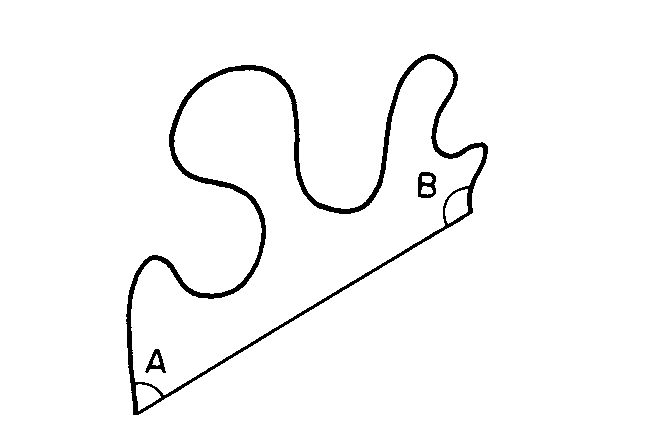
\includegraphics[scale=1]{fig1-17}
\caption{Relate the angles $A$ and $B$ to the total turning over the arc.}
\end{center}
\end{figure}


\item Fill in the details in the first proof of the \textsc{poly} closing theorem (see
``sketch of proof 1''), including a proof that the vertices of \textsc{poly} lie on a
circle.  
\item Prove that if the angle input to \textsc{poly} is an irrational number, the
turtle never returns to its initial position, and yet always remains within
a finite distance from it. [A]
\item $[P]$ lnvent some variations on the \textsc{polyroll} program, perhaps modeled
after \textsc{polyspi} and \textsc{inspi}.
\item Rewrite the \textsc{polystop} program recursively, so that it doesn't use the
\textsc{repeat} command. [A]
\item What is the sum of the interior angles of an $n$-gon? What is the
interior angle of a regular $n$-gon? Show how these formulas can be easily
derived by using the simple-closed-path theorem.  
\item Suppose we have a simple arc (an arc that does not cross itself) and
that we join the endpoints of the arc by a straight line. Suppose further
that the line and the arc do not intersect except at the endpoints (figure
1.17).  Use the simple-closed-path theorem to give a formula relating the 
total turning over the arc to the (interior) angles that the arc makes with
the line.  
\item Apply the result of the previous exercise to find the angle between a
chord of a circle and the arc that it subtends (figure 1.18a). [A]
\item Use the previous exercise to compute the arc of a circle subtended by
an inscribed angle (figure 1.18b). [HA]
\item Proof 1 of the \textsc{poly} closing theorem was based on the fact that the
vertices of a \textsc{poly} all lie on a circle. Use the simple-closed-path theorem
to show that the amount of arc on the circumscribed \textsc{poly} circle from
one vertex to the next is just the angle input to the \textsc{poly} procedure. [H]
\item We said that we would delay giving a proof of the simple-closed-path
theorem until chapter 4. Give a proof of the theorem in the special case
where the simple closed path is a \textsc{poly} figure. [H]
\item If you take a bicycle and lock the front wheel at angle $\theta$ from straight
ahead (where $\theta$ is rather small), the bicycle will turn in a circle. What
is the radius of the circle, given that the length between wheel centers
of the bicycle is D?  
\end{enumerate}

\section{Looping Programs}


\begin{figure}
\begin{center}
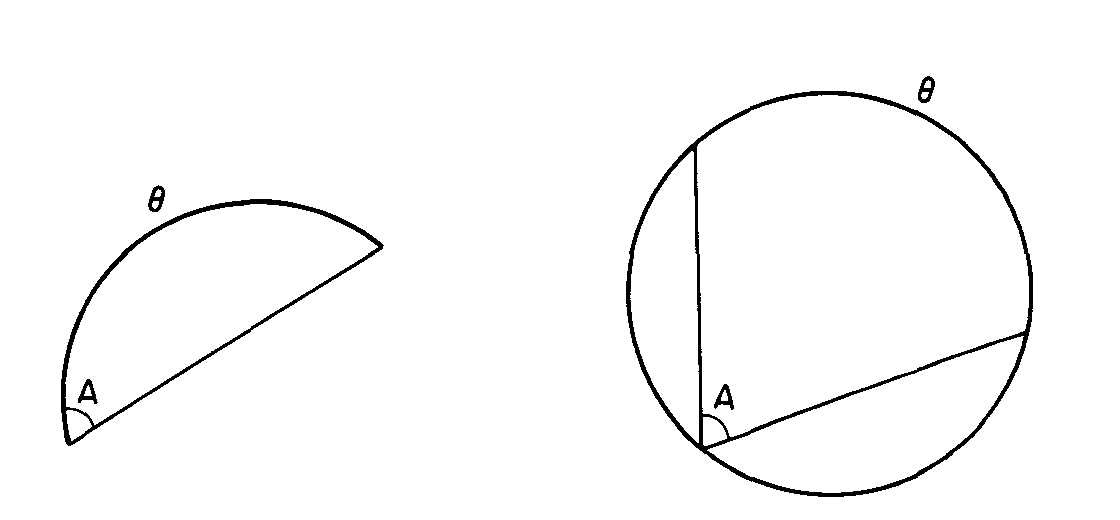
\includegraphics[scale=1]{fig1-18}
\caption{Solve for $A$ in terms of $\theta$}
\end{center}
\end{figure}


We said that the turtle approach allows us to take concepts that are
useful in thinking about computation and apply them to the study of
geometry. One such concept is that of state. Of course the idea of state
is not unique to computer science. It is important in physics, chemistry,
and any other field involving configurations that are subject to change.
But we do not generally look upon geometry in this way; geometric
figures are usually regarded as static objects. Turtle geometry provides
a more dynamic perspective --- the geometry is tied to movements.
The state of the turtle is given by specifying its position and its
heading. From the state point of view, the basic turtle commands --\textsc{forward}, \textsc{back}, \textsc{left}, and \textsc{right} --- are {\em state-change operators}: They
cause the turtle to change state. In this section we will look at a sequence
of turtle commands purely in terms of its net effect in changing the initial
state to the final state, ignoring what comes between. Thus, a sequence
of turtle commands can be summarized as a single state-change operator.
At this level of abstraction all programs that generate a closed path are
the same --- they are all {\em state-change-equivalent}. They correspond to the
simplest of all state-change operators, the one that does nothing and
leaves the initial state {\em invariant}.

\subsection{The Looping Lemma}



There is something striking about the paths drawn by the modifications
to \textsc{poly} discussed at the end of section 1.1. It is as if their descent
from \textsc{poly} cannot be suppressed! You should have noticed the same
phenomenon in many of your own programs. Figure 1.19 shows a \textsc{poly}
skeleton in dotted lines underlying the elaborate surface structures of
\textsc{newpoly} and \textsc{inspi}. Can we understand this phenomenon?

The key observation is this: Between successive vertices of the \textsc{poly}
skeleton, the program does the same thing. We might say that the
program is just a decorated version of the underlying \textsc{poly}. That the
paths of \textsc{newpoly} and \textsc{inspi} consist of a collection of identical pieces
is evident from the pictures they draw. In the case of \textsc{newpoly} the
repetitive or looping behavior is clear in the program structure. \textsc{inspi}'s
program structure will require a second look. For now we proceed on
the basis of the visual evidence of the paths and consider the class
of programs that do the same thing over and over, regardless of the
complexity of the basic loop (the thing that is repeated).

\begin{figure}
\begin{center}
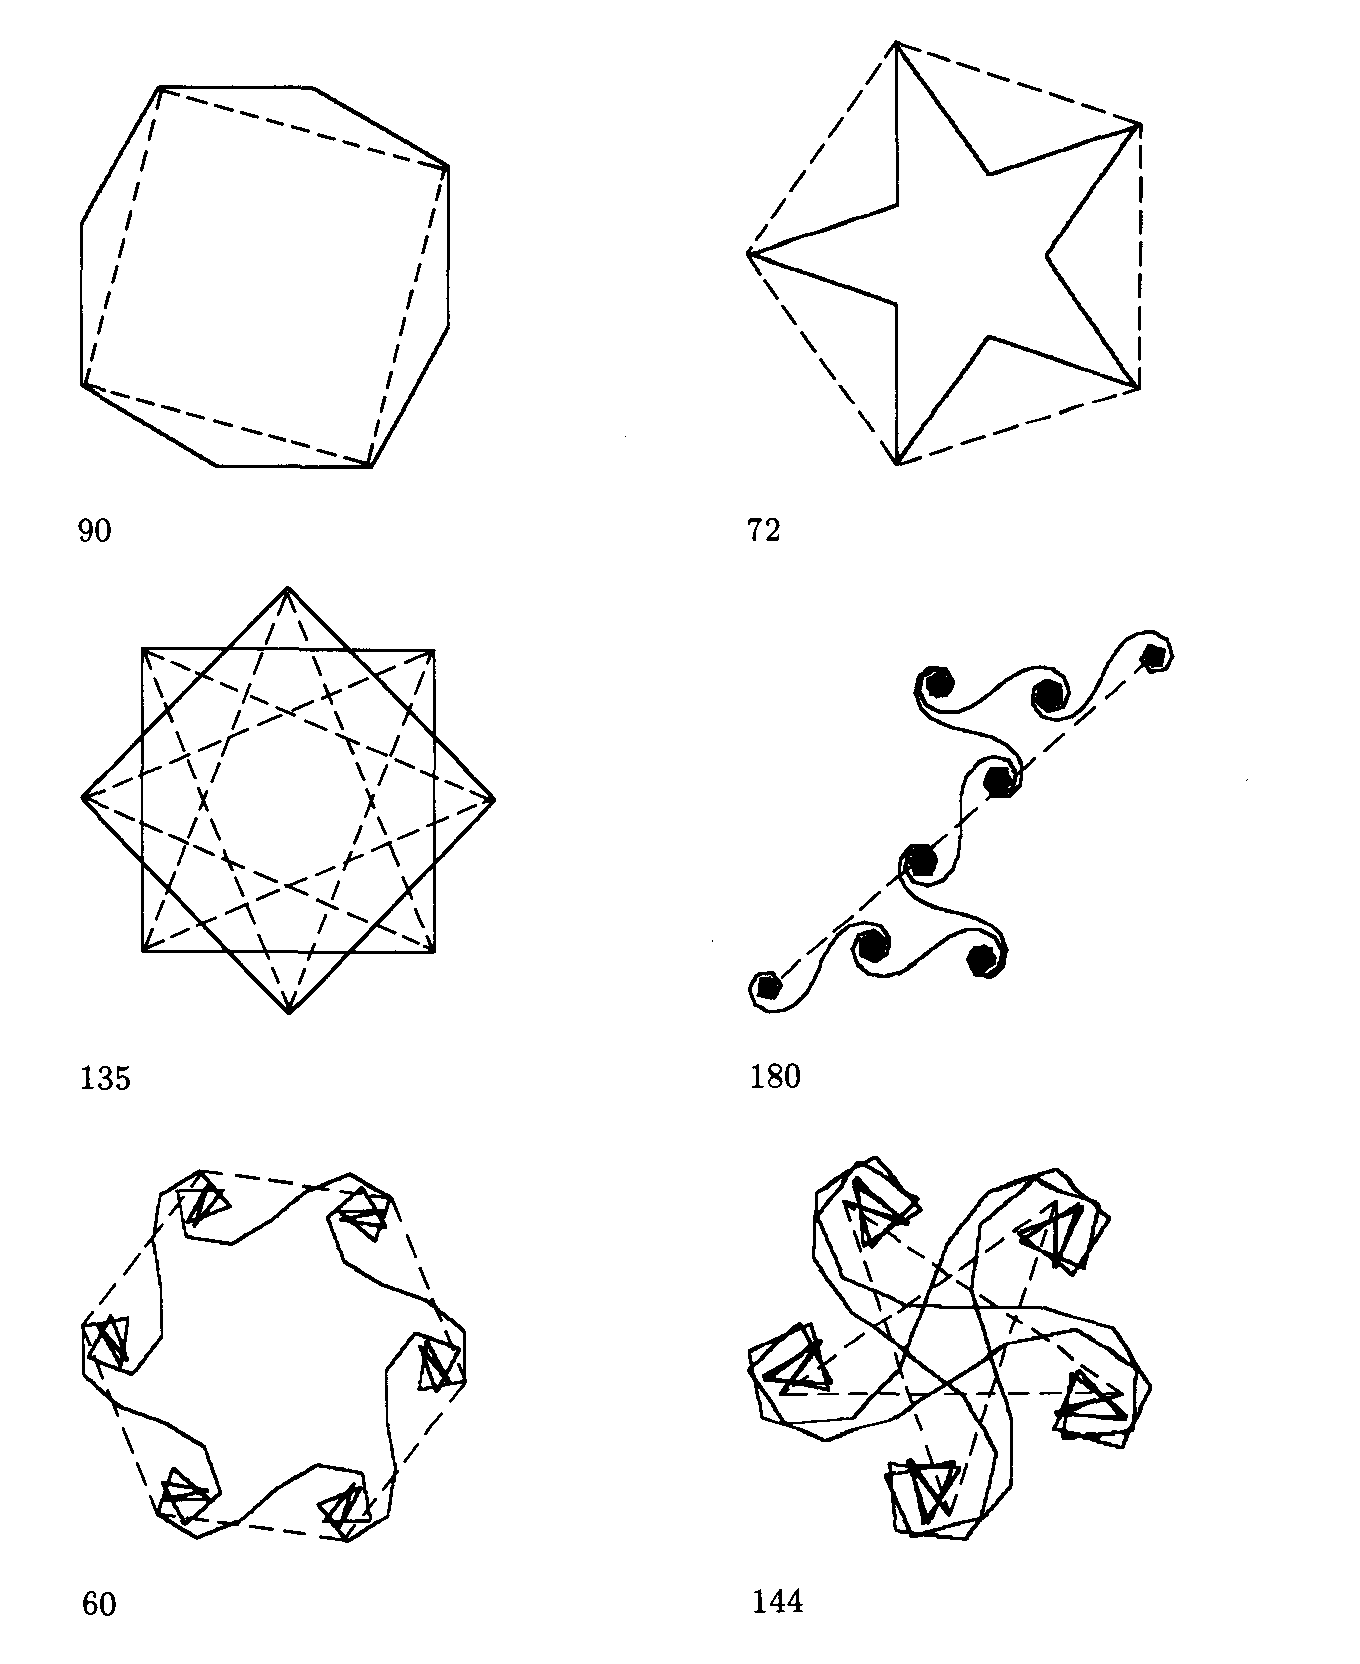
\includegraphics[scale=1]{fig1-19}
\caption{\textsc{newpdly}s and \textsc{inspi}s with ``\textsc{poly} skeletons'' indicated by dashed lines. (Numbers are skeleton angles.)}
\end{center}
\end{figure}

We can peel away the decoration by focusing on the net result of the
basic loop. What is the difference between the initial state and the final
state of the turtle? By the nature of the turtle only two things can
happen: a net change of position and a net change of heading. Figure
1.20a shows the general case. Notice that we cannot assume that the
change of position is in the same direction as the turtle's original heading;
hence, we must include an angle $i$ between the initial heading and the
change-of-position line.

\begin{figure}
\begin{center}
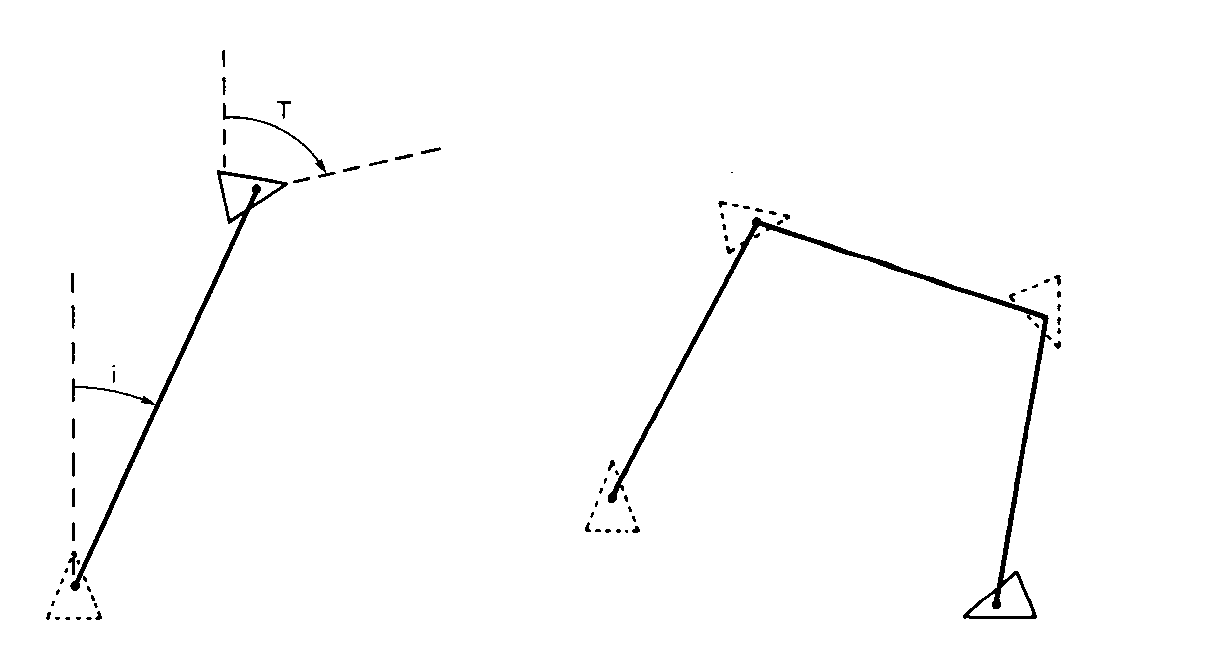
\includegraphics[scale=1]{fig1-20}
\caption{(a) The net result (state change) of some basic loop. (b) Repeating the net result
lays down the \textsc{poly} skeleton}
\end{center}
\end{figure}

When the basic loop is repeated, the same change of state must occur,
but now relative to the new heading and hence rotated by the heading
change which the turtle underwent in the first loop. We will call this
change of heading $T$ (for total turn). The next loop must follow the same
pattern, and so on. Figure 1.20b shows the repeated process laying down
the skeleton \textsc{poly}. The angle $i$ is irrelevant to the intrinsic properties of
the underlying \textsc{poly}-it just determines the relative orientation of the
\textsc{poly} with respect to the initial heading of the turtle. The important
quantity is the heading change from beginning to end of the basic loop,
the total turning $T$ in the basic loop. This is the angle of turning from
one segment of the \textsc{poly} to the next, and it determines the iigure's
properties. We can state this result more formally:

\vspace{0.5cm}

\noindent \textbf{Looping Lemma} Any program that is just a repetition of some basic
loop of turtle instructions has precisely the structure of \textsc{poly} with an
angle input equal to $T$, the total turning in the loop.

\vspace{0.5cm}

You should be able to say what ``has the structure of \textsc{poly}'' means in
detail. lt includes such things as repeatedly touching base with a circle
if total turning is not equal to a multiple of $360^{\circ}$, and touching base
with a line if it is. It also includes the fact that the symmetry type of
the figure is the same as that of the underlying \textsc{poly}. For instance, if
the total turning of the basic loop is $90^{\circ}$, the repeated loop will have the
fourfold symmetry of a square, necessarily closing in four iterations of
the loop.

\subsection{Examples of Looping Programs}

Let's analyze some simple looping programs. In \textsc{newpoly} the total
turning is $3 \times$ \textsc{angle}. If \textsc{angle} is 144, then $T = 3 \times 144 = 432$, which is
equivalent to $72 = 360 \div 5$. Hence, the five-pointed star \textsc{newpoly} actually
has the structure of a pentagon (not a \textsc{poly} with \textsc{angle 144}) --- something
that might not have been apparent from just looking at the path. (The
fact that the path is simple is a clue. Also, observe that the program
visits the vertices of the underlying pentagon in sequence, as does \textsc{poly}
with an \textsc{angle} of 72, rather than skipping between vertices, as does \textsc{poly}
with \textsc{angle} 144.)

\indent
Let's take a look at \textsc{inspi} --- in particular \textsc{inspi} with \textsc{angle} equal to
2 and \textsc{increment} equal to 20, which draws the decorated five-pointed
star shown in figure 1.12. The program simply alternates \textsc{forward side}
with turning \textsc{right} an ever-increasing angle which is tabulated in the
following:

\begin{verbatim}
RIGHT 2
RIGHT 2 + 20
RIGHT 2 + 2*20
RIGHT 2 + 3*20
.
.
.
RIGHT 2 + 17*20
RIGHT 2 + 18*20 = 2 + 360
\end{verbatim}

The last command has the same effect as the first, and the one to follow,
\textsc{right} $2 + 19 \times 20 =$ \textsc{right} $2 + 20 + 360$, is the same as the
second. The program is clearly staging a repeat performance of the first
18 steps. Computing the total turning, we find

\begin{figure}
\begin{center}
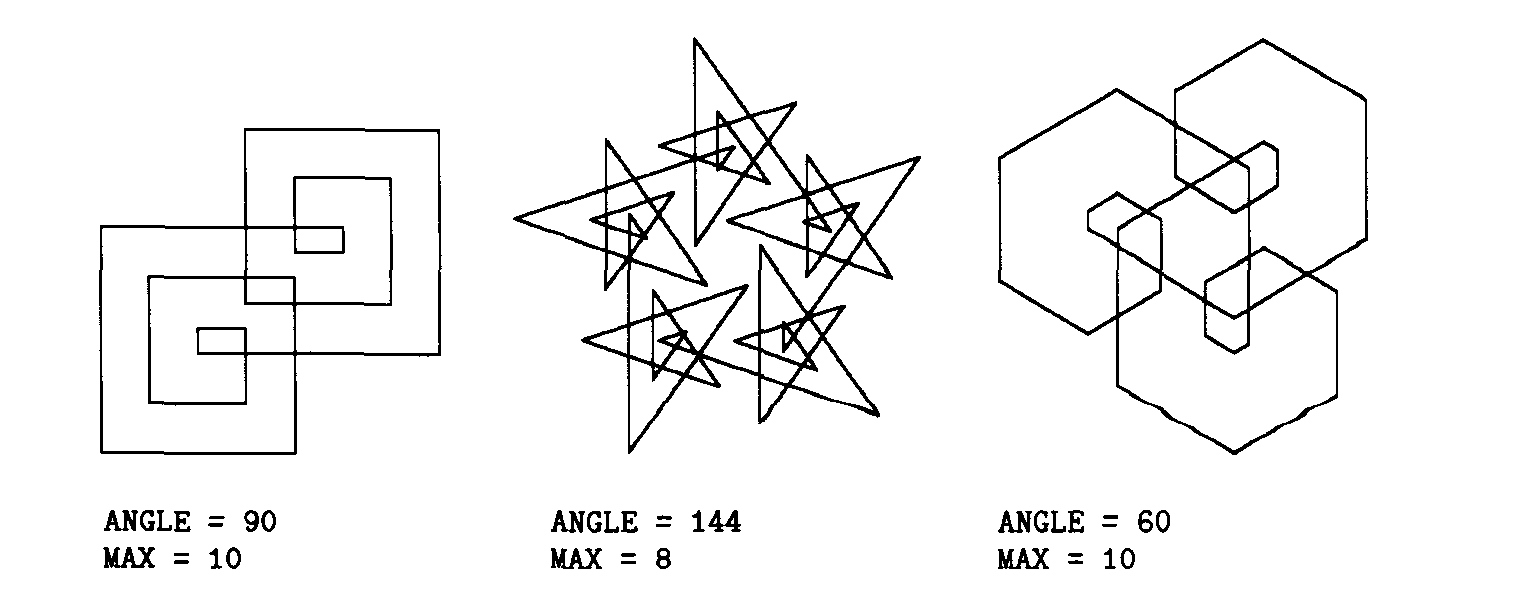
\includegraphics[scale=1]{fig1-21}
\caption{Spirolaterals}
\end{center}
\end{figure}

We will refer to the figures drawn by \textsc{spiro} as simple spirolaterals. A
more general kind of spirolateral (shown in figure 1.22) maintains a basic
loop in which each vertex has the same amount of turning, but allows the
turtle to turn left rather than right at some of the vertices. To specify
these figures we need to indicate the direction of the turtle's turning
at each vertex. The corresponding \textsc{gspiro} procedure takes four inputs:
a side length (the length of the shortest side in the figure), an angle
through which the turtle turns left or right at each vertex, a number
\textsc{max} telling how many steps are in the basic loop, and a list of numbers
specifying the vertices at which the turtle should turn left. If the vertex
number is a member of the list, then the turtle turns left at the vertex;
otherwise the turtle turns right. (The \textsc{member} command is used to tell
whether or not something is a member of a list.) Thus, the \textsc{gspiro}
procedure is

\begin{figure}
\begin{center}
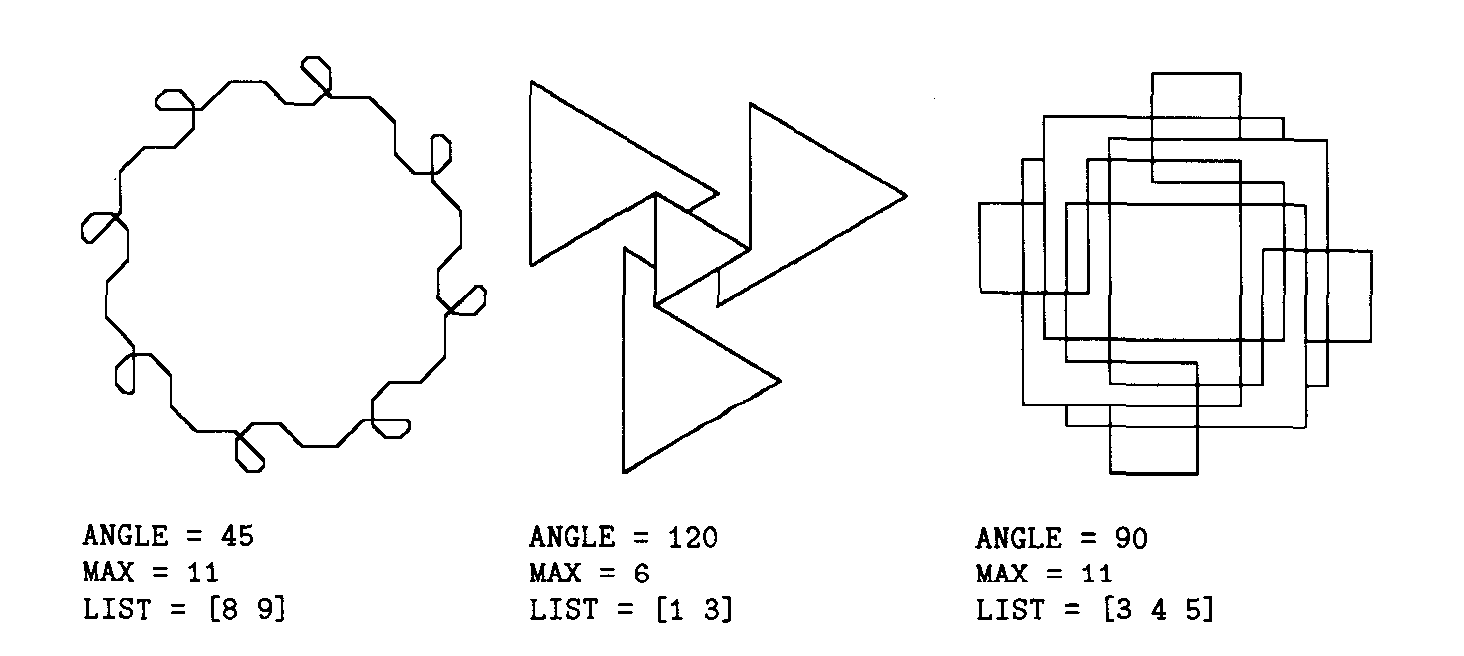
\includegraphics[scale=1]{fig1-22}
\caption{Generalized spirolaterals}
\end{center}
\end{figure}

\begin{verbatim}
TO GSPIRO (SIDE, ANGLE, MAX, LIST)
   REPEAT FOREVER
      SUBGSPIRO (SIDE, ANGLE, MAX, LIST)

TO SUBGSPIRO (SIDE, ANGLE, MAX, LIST)
   COUNT <- 1
   REPEAT
      FORWARD SIDE * COUNT
      IF MEMBER (COUNT, LIST)
         THEN LEFT ANGLE
         ELSE RIGHT ANGLE
      COUNT <- COUNT + 1
   UNTIL COUNT > MAX
\end{verbatim}
\begin{figure}
\begin{center}
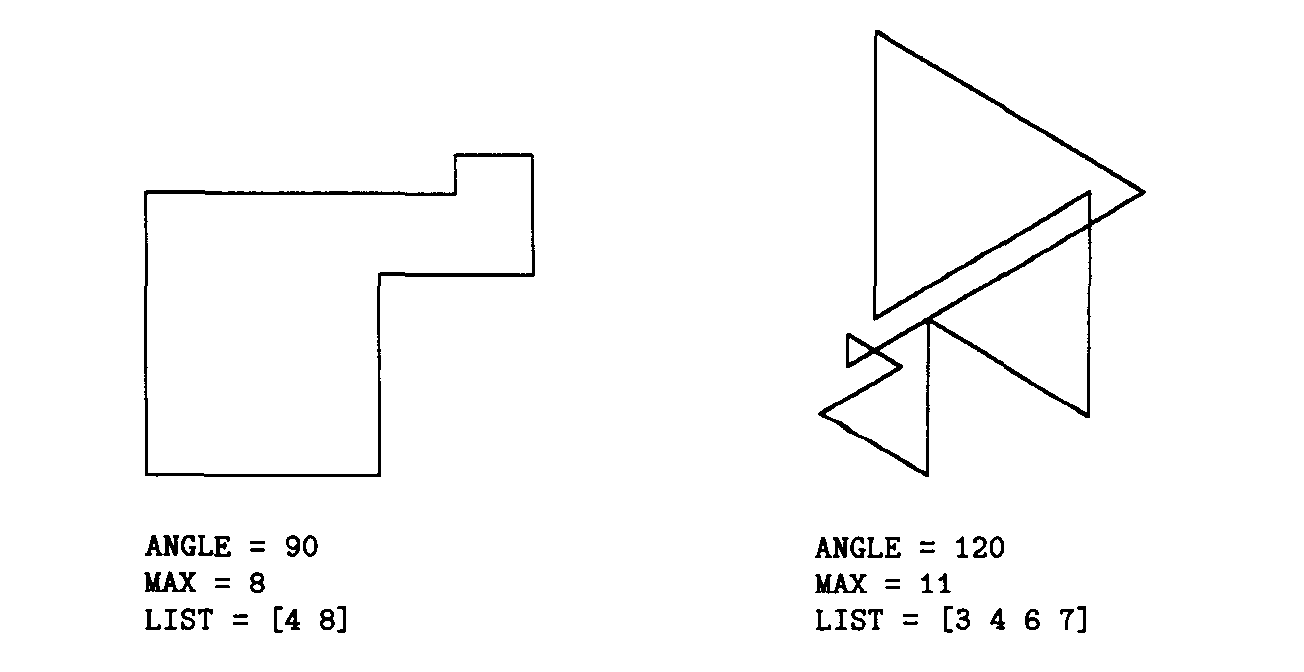
\includegraphics[scale=1]{fig1-23}
\caption{Unexpectedly closed spirolaterals}
\end{center}
\end{figure}

The basic loop \textsc{subgspiro} makes \textsc{max} $-$ $L$ right turns and $L$ left turns
where $L$ is the number of elements in \textsc{list}, making a total turning of
(\textsc{max} $-$ $L$) $\times$ \textsc{angle} $-$ $L$ $\times$ \textsc{angle} $=$ (\textsc{max} $- 2L$) $\times$ \textsc{angle}.
One intriguing property of spirolaterals is that they may be closed even
when the heading change is a multiple of $360^{\circ}$. Total turning a multiple
of $360^{\circ}$ would lead you to expect a \textsc{poly} substrate that would march
off on a straight line to infinity. But, by a remarkable coincidence, the
sidelength of the underlying \textsc{poly} (which we did not bother to compute
for any of these other programs) might turn out to be 0 as well! This
corresponds to having a looping program in which the basic loop closes
all by itself. This phenomenon deserves a name: {\em unexpectedly closed}. Figure 1.23 gives some examples of unexpectedly closed spirolaterals.

\subsection{More on the Looping Lemma}

We end the body of this section with two remarks about the looping
lemma --- one about its implications beyond predicting the symmetry of
looping programs, the other about increasing the strength of the lemma.
First, the looping lemma constrains the behavior of any looping program. Under many circumstances, it may be possible to exclude simple
looping as a way of generating a class of paths. For example, any infinite
spiral neither touches base on a lixed circle nor marches off to infinity
around a line as \textsc{poly} does, so it cannot be drawn by any looping program.

Second, it can be very valuable to know how to identify which programs are looping programs without a detailed look at each particular
case. We can give a purely program-structural criterion that serves to
identify such programs: A program must loop (or terminate) if it consists
of any combination of

\begin{itemize}
\item fixed and finite sequences of turtle commands \textsc{forward}, \textsc{back}, \textsc{left},
and \textsc{right} with specified numeric inputs (these are called fixed instruction sequences),
\item repeats, and
\item calls to programs that satisfy these properties.
\end{itemize}

Notice that this criterion is recursive in form.

\subsection{Technical Summary}

The following is a technical recap of results stated or implied in this
section. The detailed proofs of these facts are left as exercises.

\subsubsection{The Canonical Form of a Turtle State-Change Operator}

Any fixed instruction sequence of turtle commands is state-change-equivalent to a \textsc{poly} step sandwiched between a \textsc{right} I  and \textsc{left} I  for some angle I:

\begin{verbatim}
RIGHT I
FORWARD D
RIGHT T
LEFT I
\end{verbatim}
The angle $T$ is precisely the total turning of the fixed instruction sequence.

\subsubsection{Looping Lemma and Classification of Looping Programs}

Any program that repeats a fixed instruction sequence (or the equivalent,
as in \textsc{inspi}) has the behavior of a \textsc{poly} with angle $T$ and side $D$ in the
following senses (the angle $T$ may be simply determined as the total
turning in the basic loop):

\noindent \textbf{Boundedness} If $T \not= 0$ then the figure drawn by the program will lie
within a fixed distance from some circle, and hence will be bounded. In
the exceptional case, $T = 0$, the figure will lie within a fixed distance
from some line (figure 1.24).

\begin{figure}
\begin{center}
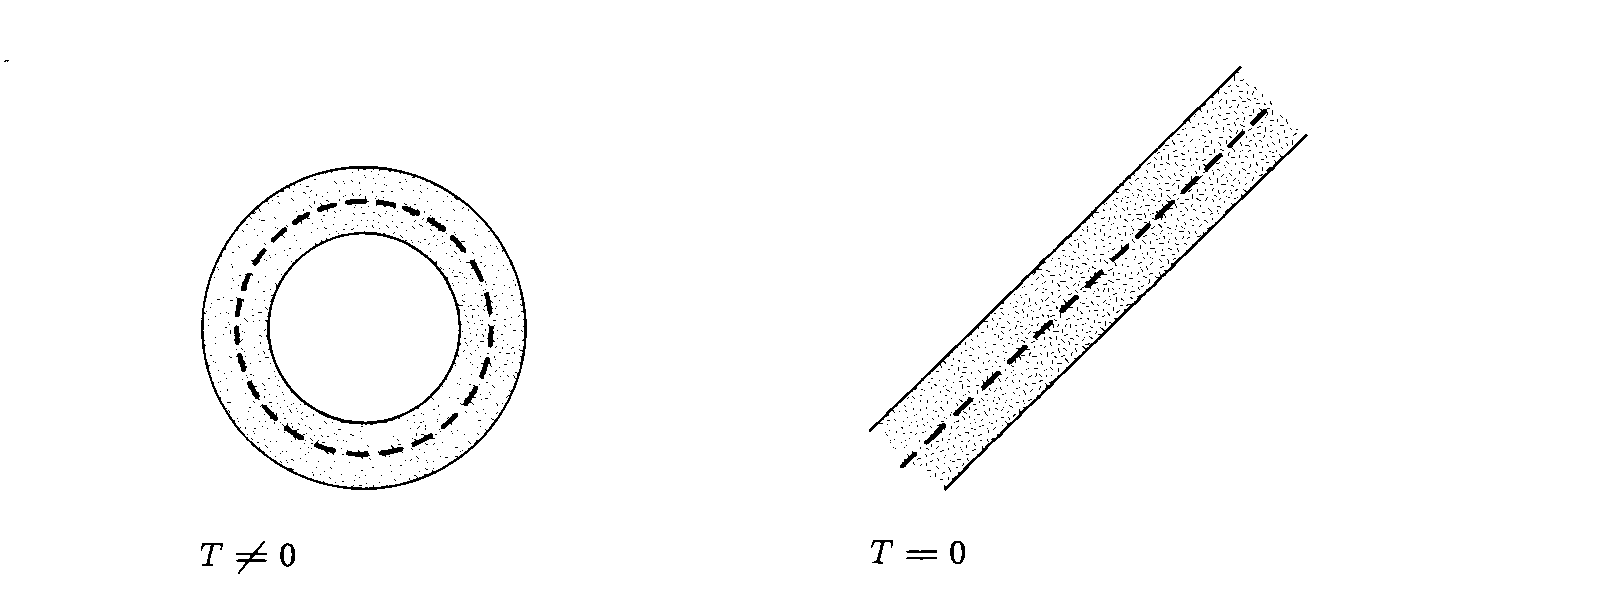
\includegraphics[scale=1]{fig1-24}
\caption{Any looping program is confined to a region (a) near a circle ($T \not= 0$) or (b) in the exceptional case ($T = 0$) near a line.}
\end{center}
\end{figure}

\noindent \textbf{Closing} If $T$ is a rational multiple of $360^{\circ}$, the program will always
draw a closed path, with the usual exception, $T = 0$, which causes the
program to walk off to infinity. The exception to the exception is when
$D$ is also zero, the equivalent of \textsc{poly 0 0}, in which case the program is
``unexpectedly'' closed. If $T$ is irrational the program will never close.

\noindent \textbf{Symmetry} The program must have the same rotational symmetry as
\textsc{poly d t}. In particular, if $T = 360s/r$ where $s/r$ is a fraction in lowest
terms, then the program will have $r$-fold symmetry. (We have not yet
discussed symmetry in detail. This topic will form the basis of section 1.4.)

\subsection{Nontechnical Summary}

Doing the same thing over and over is either circular, straight-linish, or
very dull.

\subsubsection{Exercises for Section 1.3}
\begin{enumerate}
\item $[P]$ Draw at least three distinct (ignoring size) \textsc{inspi} figures with
sixfold symmetry.
\item Give a proof of the looping lemma and the classification of looping
programs given in the technical summary. This may be done using the
form of a general state-change operator (given above) or by modifying
Proof 2 of the \textsc{poly} closing theorem of subsection 1.2.2. Give bounds
for the ``fixed distances'' specified in the boundedness part in terms of
the instructions in the basic loop.
\item $[P]$ Figure 1.23 shows some unexpectedly closed spirolaterals. Find
some more.
\item What is the heading change for \textsc{inspi} with an \textsc{angle} of $A$ and an
\textsc{increment} of 10? [A]
\item $[D]$ What is the heading change for \textsc{inspi} with an \textsc{angle} of $A$ and
an \textsc{increment} of 360/$n$, where $n$ is an integer? [HA]
\item $[DP]$ Compute the total turning, $T$, of the basic loop in the following
looping program in terms of the angle inputs \textsc{bottom} and \textsc{top}. Use
your formula to draw at least three different (ignoring size) figures with
threefold symmetry; fourfold, fivefold.  

\begin{verbatim}
TO POLYARC (SIDE, BOTTOM, TOP)
   REPEAT FOREVER
      INSPI.STOP (SIDE, BOTTOM, TOP, 1)
      INSPI.STOP (SIDE. TOP, BOTTOM, -1)

TO INSPI.STOP (SIDE, START.ANG, END.ANG, INC)
   REPEAT
      FORWARD SIDE
      LEFT START.ANG
      START.ANG <- START.ANG + INC
   UNTIL START.ANG = END.ANG
\end{verbatim}
\item $[P]$ Make ``even more general'' spirolaterals by allowing the turtle to
move \textsc{back} at certain of the vertices. Analyze this program. Find some
unexpectedly closed figures.
\item $[DD]$ Show that a simple spirolateral can never be unexpectedly
closed.  
\item $[DD]$ Can \textsc{inspi} produce unexpectedly closed figures?
\item $[P]$ Invent some disguised looping programs like \textsc{inspi}. Give a
formula for the total turning of the basic loop in terms of the inputs
to the procedure. Find inputs that draw figures with simple symmetry.
Find inputs that draw unbounded figures. Determine whether any of
these figures are unexpectedly closed.

\item When we summarize turtle paths as state-change operators, the
closed paths are precisely those operators that leave the turtle's state
unchanged. This suggests the generalization of studying operators that,
when run twice (or three times, and so on), leave the state unchanged.
Describe the paths corresponding to these operators. [A]

\item $[P]$ Can you characterize ``looping programs'' in terms of the commands used in writing them? In particular, consider the following program structures, where X and Y are variables and n is some fixed number:
\begin{itemize}
\item do loops
\item goto statements
\item assignment statements of the form $X \leftarrow n$
\item assignments of the form $X \leftarrow Y + n$
\item conditional statements of the form \textsc{if} $X = n$ . . .
\end{itemize}
\end{enumerate}
\indent
For each kind of structure, say whether a program that repeats a block
of instructions consisting of basic turtle commands together with that
particular structure must necessarily be equivalent to a program which
repeats a fixed instruction sequence. Are there bad combinations, in the
sense that two structures which separately lead to looping may not loop
when combined in a single program?

\subsection{Symmetry of Looping Programs}

Section 1.3 showed how the symmetry of any looping program is determined by the symmetry of an underlying \textsc{poly} skeleton. But what determines the symmetry of the \textsc{poly}? To begin with, it is clear that the \textsc{side} input in \textsc{poly side angle} does not aiiect the shape of the figure at all but only determines the size. The real question is: How does the \textsc{angle} input affect the symmetry of \textsc{poly}? To be more precise, we can break this question into two questions:

For a given \textsc{angle} input, how many vertices will the resulting \textsc{poly} have?
Conversely, if we want to produce a \textsc{poly} with a specified number of
vertices, what number(s) can we use for the \textsc{angle} input?

The purpose of this section is to answer these questions, and in doing so
to provide a taste of the mathematics of number theory.

\subsection{The Symmetry of \textsc{poly}}

We want to relate the number of vertices, $n$, to the input \textsc{angle}, which
we'll call $A$ for short. The \textsc{poly} closing theorem of 1.2.2 gives us a very
good start. It says \textsc{poly} is done when the turtle has turned a multiple
of $360^{\circ}$, that is, when $n$ turns of $A$ each is some multiple of 360:

$nA = 360R$

We've given the multiple the name $R$ for a good reason: It is the rotation
number of the figure, as defined in subsection 1.2.1.

But the above equation, which defines a common multiple of $A$ and
360, doesn't tell the whole story. $R$ and $n$ aren't just any integers
satisfying the equation; they are the smallest (positive) that do so,
corresponding to the first time heading change reaches a multiple of 360.
That is why the number $nA=360R$ is called the {\em least common multiple}
of $A$ and 360, denoted LCM(A, 360). The answer to our first question is:
For an \textsc{angle} input of $A$, the number of vertices of the resulting \textsc{poly} is
$n$ = LCM(A, 360) / $A$ and the rotation number is $R$ = LCM(A, 360) / 360.

What we've done so far is little more than giving the answer a name.
How does one go about computing the least common multiple? One way,
which assumes that $A$ is an integer, is to express $A$ and 360 as products
of primes. Then each of the expressions {\em nA} and 360$R$ will give a partial
view of the factorization of LCM(A, 360). For example, if $A$ = 144 then
we have $A$ = $2^4 \times  3^2$, 360 = $2^3 \times 3^2 \times 5$. Using this decomposition, we
can deduce that
$$\operatorname{LCM}(144,360) = n \times 2^4 \times 3^2 = R \times 22 \times 32 \times 5 = 2^4 \times 3^2 \times 5 = 720$$
\noindent for it is easy to see that the LCM must contain at least four factors
of 2 (from $A$), one factor of 5 (from 360), and two factors of 3 (from
either $A$ or 360), and from this we derive that $n$ = 5 and $R$ = 2.
So \textsc{poly 100 144} has fivefold symmetry (it consists of $n$ = 5 identical
pieces identically hooked together) and rotation number 2.

Another way to compute the least common multiple is to solve the
equation {\em nA} = 360$R$ exactly as the procedure \textsc{poly} solves it: by running until it closes! Make a list of $n$ $\times$ $A$ for $n$ = 1,2,3,... and see
when $n$ $\times$ $A$ is a multiple of 360. Applying this method to our example
$A$ = 144 gives

\begin{tabular}{l c r} 
$n$ & {\em nA} & multiple of 360? \\
\hline
1 & 144 & no \\
2 & 288 & no \\
3 & 432 & no \\
4 & 576 & no \\
5 & 720 & yes \\
\end{tabular}

We can formulate this method as a procedure for computing the least
common multiple:

\begin{verbatim}
TO LCM A B
   N <- O
   REPEAT
      N <- N + 1
      MULTIPLE <- N * A
   UNTIL REMAINDER (MULTIPLE, B) = 0
   RETURN MULTIPLE
\end{verbatim}
Such ``brute force'' methods of computation can be very useful. We will
see in the next subsection the utility of a simple modification of this
process, called Euclid's algorithm. The \textsc{lcm} procedure uses \textsc{return} --- a
command we haven't seen before. Since the procedure is supposed to
be computing some value, we need to have some method for ``getting
the value out of the procedure.'' This is what \textsc{return} does. In practice
the returned value will be used as an input to another operation, for
example, \textsc{print LCM(144,360)}.

Let's turn to our second question about the symmetry of \textsc{poly} figures.
Suppose we want to produce figures of a given symmetry; what \textsc{angle}
can we use? To answer this question, let's start again with the basic
symmetry equation {\em nA} = 360$R$. Since we want to find values for $A$ that
will produce a given value for $n$, we should be able to use any $A$ that
satisfies $A$ = 360$R$/$n$. The question is: What value(s) can we choose
for $R$? For instance, we can take $R$ = 1, $A$ = 360/$n$, which always
works --- it makes a regular {\em n-sided polygon}. But $R$ = 2, $A$ = 2 $\times 360 / n$
may not work. Here's an example: Suppose we want tenfold symmetry,
$n$ = 10. If we take $R$ = 2, then $A$ will be 72. This makes a pentagon,
not a figure with tenfold symmetry.
We've been fooled. $A = 360R/n$ doesn't always give $n$-fold symmetry.
Let's look more carefully at the above guess, $R$ = 2, $n$ = 10.

Not only does the resulting pentagon not have tenfold symmetry, but it
has rotation number 1, not 2. We clearly are not justified in naming our
guesses 10 by $n$ and 2 by $R$, so let's give them new names, {\em n'} and {\em R'}.
How do these relate to the real $n$ and $R$?

Let's compute the real n and R that correspond to $A$ = 360{\em R'}/{\em n'}. We
want the smallest positive integers $n$ and $R$ that satisfy {\em nA} = 360$R$. But
this equation is satisfied by all pairs of integers $R$ and $n$ with the property
that $R$/$n$ = {\em R'}/{\em n'}. Since we want $R$ and $n$ to be the smallest pair with
this property, we should take them to be the numerator and denominator
of the fraction {\em R'}/{\em n'} reduced to lowest terms. In our example we had
{\em R'}/{\em n'} = 2/10 = 1/5, so $n$ = 5 and $R$ : 1. To put this another way,
$A$ = 360{\em R'}/{\em n'} will give {\em n'}-fold symmetry only when {\em R'}/{\em n'} cannot be
reduced, that is to say, when {\em R'} and {\em n'} have no factors in common.
Thus, the answer to the second question above is the following:

To generate a \textsc{poly} with $n$-fold symmetry, take the \textsc{angle} input to be
$A = 360R/n$, where $R$ is any positive integer that has no factors in
common with n.

\subsection{Common Divisors}

We've answered our questions about the symmetry of \textsc{poly} in terms of
such concepts as common multiples and common factors. Let's take a
detour from turtle geometry and turn this process around to see what
knowing about \textsc{poly} can tell us about these number-theoretic concepts.

To begin with, the previous subsection led us to consider pairs of
integers $n$ and $R$ that have no common factors. Such pairs are called
relatively prime. We saw that $A = 360R/n$ draws an $n$-sided \textsc{poly}
precisely when $R$ is relatively prime to $n$. We'll reinterpret this fact in
terms of a new way of looking at the \textsc{poly} process.

Think of the $n$ vertices of \textsc{poly} lying on a circle and numbered from 0
through $n - 1$. To construct the various $n$-sided \textsc{poly}s we can connect
the vertices in sequence using the following sorts of rules: (1) Connect
each vertex to the very next one; (2) connect the vertices, skipping one
in between; (3) connect the vertices, skipping 2 in between; and so on.
Figure 1.25 illustrates the various patterns for $n = 8$. There are $n - 1$
possibilities, which correspond to $R$ = 1,2, . . .,$n - 1$ in the formula
$A$ = 360$R$/$n$. For any choice of $R$, if we start at the vertex numbered
0, then that is connected to the vertex numbered $R$, which is connected
to the vertex numbered 2$R$, and so on. Since we're counting these vertices modulo n, we see that the sequence of vertices hit are precisely the

\begin{figure}
\begin{center}
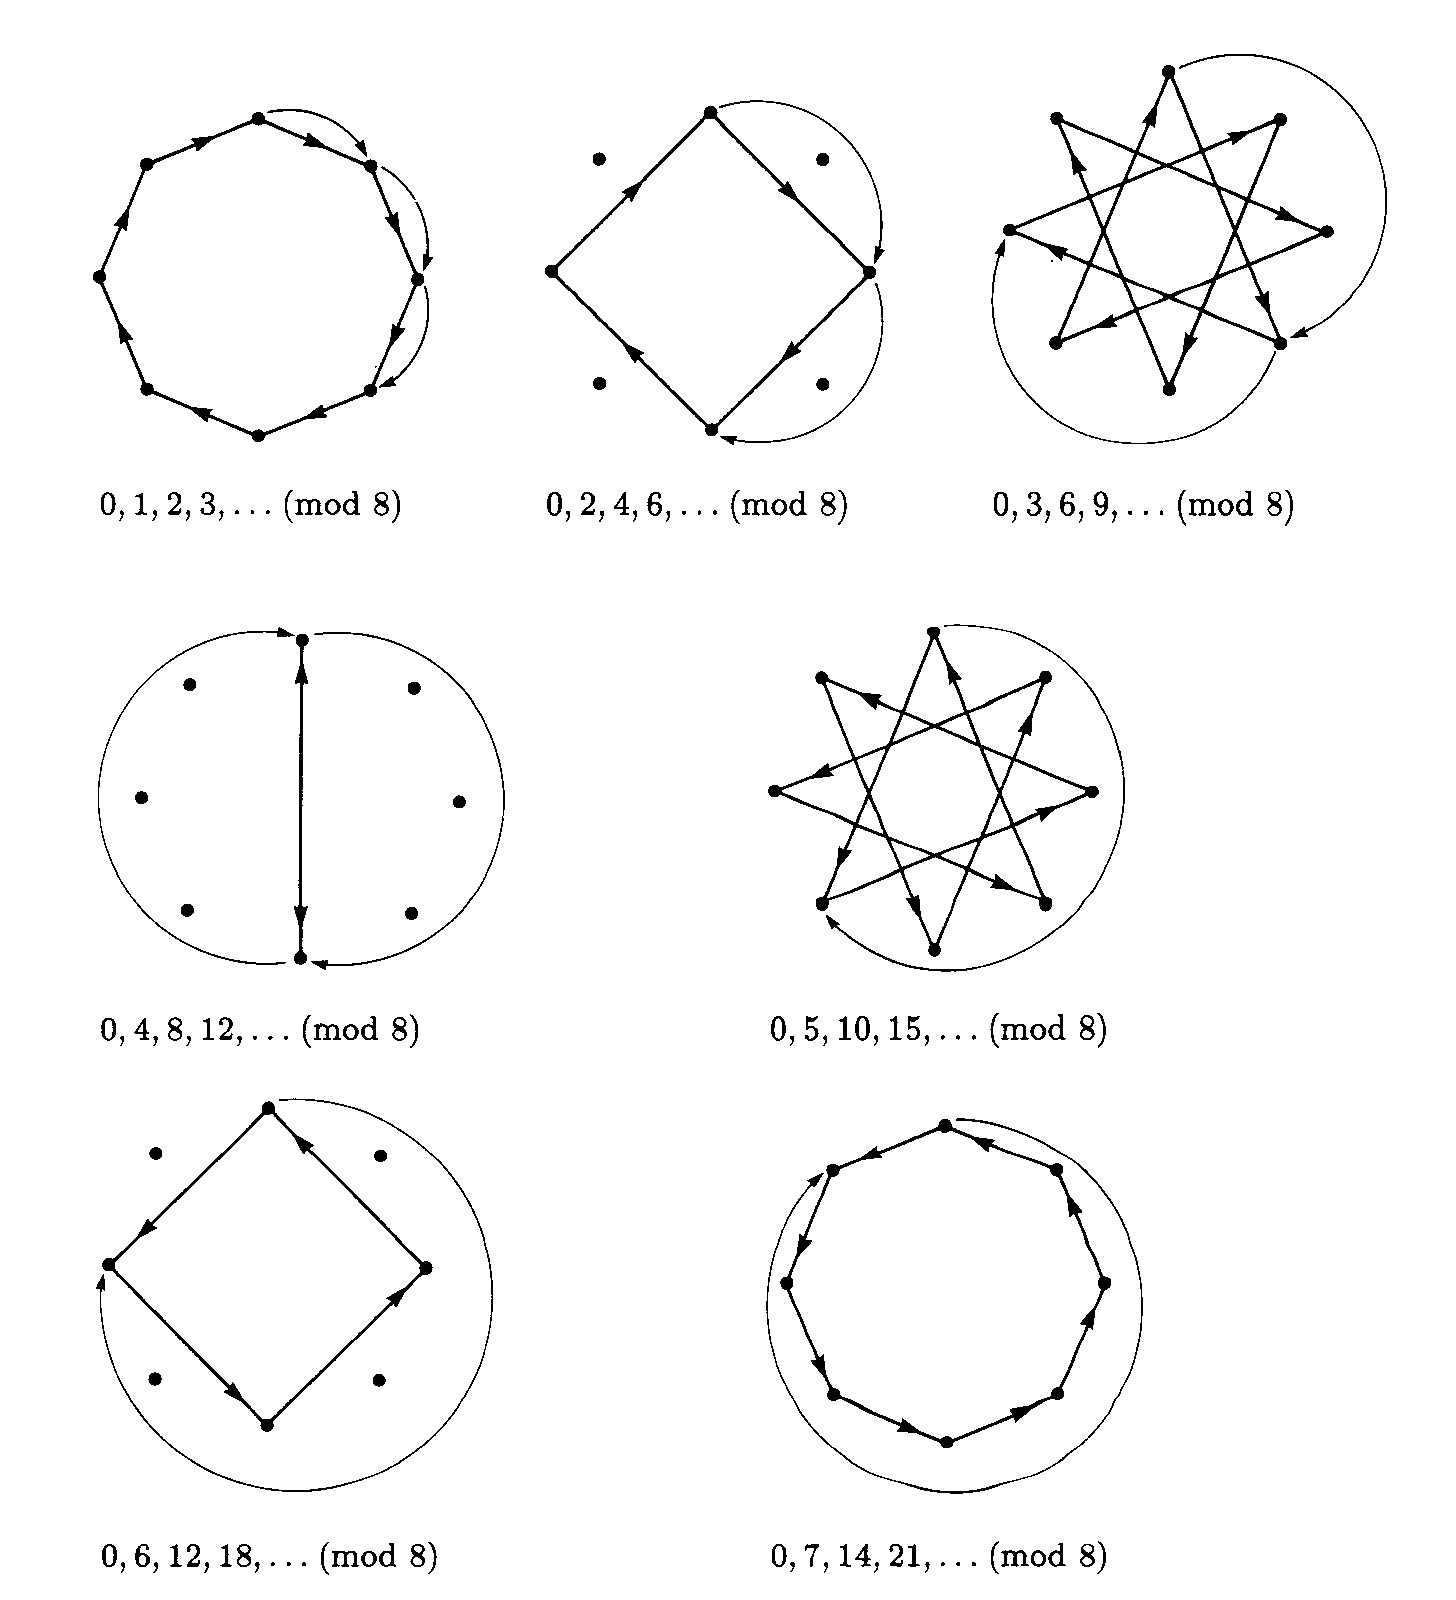
\includegraphics[scale=1]{fig1-25}
\caption{Patterns of connecting eight points, $n = 8$}
\end{center}
\end{figure}


multiples 0, $R$, 2$R$, . . . , ($n - 1$)$R$ taken modulo $n$.

Now we saw in the previous subsection that, if $R$ and $n$ are relatively
prime, then the resulting \textsc{poly} figure will have $n$ vertices. In terms of the
circle picture this means that all vertices on the circle 0, 1, 2, . . . ,$n - 1$
are reached. Consequently, if $R$ and n are relatively prime, then the
multiples of $R$ taken modulo $n$ must include all the numbers between 0
and $n - 1$. In other words, if {\em s} is any integer between 0 and $n - 1$, then
there is some multiple of $R$, say {\em pR}, with {\em pR} = {\em s} (mod $n$). Moreover, if
$R$ and $n$ are not relatively prime, then at least one of the $n$ vertices will
not be touched by the \textsc{poly} process, and so there will be some number
{\em s} which is not equal to {\em pR} (mod $n$) for any $p$. Restating the equality
modulo $n$ in terms of precise equality, we have the following: 

Two integers $R$ and $n$ are relatively prime if and only if, for any integer
{\em s}, we can find integers $p$ and $q$ such that $pR - qn = s$.

This condition can be written in an equivalent form (exercise 10) that
reflects the fact that, if the vertex labeled 1 is hit, then all vertices must
be:

Two integers $R$ and $n$ are relatively prime if and only if there exist
integers $p$ and $q$ such that $pR + qs = 1$.

In summary: We have shown how to translate a condition about the
relative primality of two integers into a rather different condition which
has to do with representing integers as sums.

What exactly happens when $R$ and $n$ are not relatively prime? Figure 
1.25 includes some examples: Taking $n$ = 8 and $R$ = 2 hits all the
even vertices (the multiples of 2); $n$ = 8 and $R$ = 4 hits only 0 and
4 (multiples of 4); $n$ = 8 and $R$ = 6 hits all the multiples of 2. In
general, the vertices which are hit --- numbered 0, $R$, 2$R$, . . . , $(n - 1)R$,
taken modulo $n$ --- give precisely the multiples of some integer $d$. This
integer $d$ is called the greatest common divisor of $n$ and $R$, and it can be
defined by stating that $d$ = GCD($n$, $R$) is the largest integer that divides
both $n$ and $R$. The fact that the vertices which are hit are precisely the
multiples of $d$ follows from the fact that GCD($n$, $R$) can alternatively
be defined as the smallest positive integer that can be represented as
{\em pR} + {\em qn}, where $p$ and $q$ also integers. We leave it to you (exercise 11)
to verify these claims. You can see that the GCD of $n$ and $R$ is an
important quantity. When it is 1, $n$ and $R$ are relatively prime and
the \textsc{poly} has $n$-fold symmetry. When the GCD is not 1, it gives $d$, the
integer whose multiples are the vertices actually hit.

Neither definition of GCD --- as the largest common divisor, or as the
smallest positive {\em pR} + {\em qn} --- seems very helpful in actually computing
the GCD of two given integers. One method for doing so is Euclid's
algorithm. The idea of the algorithm is very simple: The common factors
of $n$ and $R$ are the same as the common factors of $n - R$ and $R$. (Prove
this.) And so the problem of finding the GCD of $n$ and $R$ can be reduced
to finding the GCD of $n$ - $R$ and $R$:

\vspace{0.5cm}

\noindent \textbf{Euclid's Algorithm} Start with two numbers. (1) If the two numbers are equal, then stop; the GCD is their common value. (2) Subtract the
smaller number from the larger and throw away the larger. (3) Repeat
the entire process using, as the two numbers, the smaller number and the difference computed in step 2.

\vspace{0.5cm}

The process produces ever smaller numbers and stops with two equal
numbers. Take as an example 360 and 144. The sequence of pairs
generated is

(360,144) $\rightarrow$ (216,144) $\rightarrow$ (72,144) $\rightarrow$ (72, 72) $\rightarrow$ done: GCD = 72

Finding the GCD of 360 and 144 can be interpreted as follows: Any \textsc{poly}
with an integer angle will touch some subset of the vertices of a regular
360-gon. If the angle is 144, the vertices touched will be the multiples
of 72.

We can translate Euclid's algorithm into a recursive computer procedure:

\begin{verbatim}
TO EUCLID (N, R)
   IF N = R THEN RETURN N
   IF N > R THEN RETURN EUCLID (N - R, R)
   IF N < R THEN RETURN EUCLID (N, R - N)
\end{verbatim}
There's an obvious way to speed up the algorithm: Subtract multiple
copies of the smaller number from the larger in a single step. Even better,
we can divide the smaller number into the larger, taking the smaller
number and the remainder to start the next step. This has an additional
advantage --- we will know automatically that the remainder is smaller
than the original smaller number, so it will not be necessary to test to
see which of the two inputs is smaller:

\begin{verbatim}
TO FAST.EUCLID (N, R)
   IF N = R THEN RETURN N
   ELSE RETURN FAST.EUCLID (R, REMAINDER (N, R))
\end{verbatim}
Note that Euclid's algorithm is very nearly the reverse of the ``brute
force'' method for finding the least common multiple given in subsection
1.4.1. In fact the algorithm gives us a new way of computing the LCM
of two numbers because of the formula
$$\operatorname{LCM}(p, q) \times \operatorname{GCD}(p, q) = p \times q$$
which is true for any integers $p$ and $q$. (See exercise 16.)

As a final remark we point out that, whereas the \textsc{remainder} function
used in \textsc{fast.euclid} is defined only for integers, the operations in the
original \textsc{euclid} procedure make sense for any numbers. So we can define
the GCD for any two numbers (not just integers) to be the value returned
by the \textsc{euclid} procedure. (Exercises 15-17 invite you to investigate the
properties of this generalized GCD.) We see here how the procedural
formulation of a concept can suggest new insights and directions for
exploring. Further explorations suggested by the \textsc{euclid} procedure are
illustrated in exercises 18-25.

\subsubsection{Exercises for Section \thesection}

\begin{enumerate}
\item Determine the symmetry of \textsc{poly} with $A$ = 350, 35, 37, 12$\frac{1}{2}$, 26$\frac{2}{3}$. For
each value of $A$, find $p$ and $q$ such that $A = 360p/q$ where $p/q$ is a
fraction reduced to lowest terms. [A]
\item Using only integer angles, what are all the possible values of $n$ for
which \textsc{poly} can draw an $n$-sided figure?  
\item $[D]$ Show that the \textsc{poly} symmetry determined by \textsc{angle} = 360 - $A$
is the same as the symmetry of \textsc{angle} : $A$. What about the symmetry
of \textsc{angle} : 180 - $A$? [HA]
\item Consider the process of finding the least common multiple of $A$ and
{\em B}. Show that the ``brute force'' method will find the same minimal
number $n$ such that {\em nA} = {\em RB} as it will for {\em n(Ax)} = {\em R(Bz)} where {\em x} is
any number, and hence that LCM({\em Ax}, {\em Bx}) = {\em x} $\times$ LCM($A$, {\em B}). Use this
idea to show how to compute least common multiples of (noninteger)
rational numbers. If $A$ = $p$/$q$ and {\em B} = {\em r}/{\em s}, both fractions in lowest
terms, show how to pick sv so that one can use the prime factorization
method to compute LCM(A, B). [A]
\item We saw that $A$ = 360$R$/$n$ will produce an $n$-pointed figure for any
integer $R$ relatively prime to $n$. But how many of these $R$s actually
produce \textsc{poly}s that look different? How many different \textsc{poly}s are there
with $n$ = 10, 36, 37? How many in general? [A]
\item In solving the previous problem you may want to make use of the
Euler $\phi$ function, which is defined for positive integers $n$ to be the number
of integers less than $n$ and relatively prime to it. Euler gave a formula
for $\phi$($n$), which works as follows: Suppose that {\em $p_1$},{\em $p_2$}, $...$ are the distinct
prime factors of $n$, that is $n$ = $p_1^ap_2^b$ .... (For example, 3960 = $2^3 \times
3^2 \times 5 \times 11$.) Then
$$\phi(n) = n(1 - \frac{1}{p_1})(1 - \frac{1}{p_2})$$
\noindent Use this formula to compute $\phi$(1,000, 000). [A]
\item $[D]$ Use the fact that, for $R$ relatively prime to $n$, the multiples of $R$
include all the integers 1, 2, . . . , $n$ - 1 (mod $n$) to prove Fermat's Little
Theorem: If $p$ is a prime and $R$ is any positive integer less than $p$, then
$R^{p-1} = 1$ (mod p).  
\item $[P]$ Fermat's Little Theorem lies behind a recently discovered way to
test by computer whether large numbers are prime. The idea is to start
with a number $p$, pick a random number {\em a} less than $p$, and compute
$a^{p-1}$ (mod $p$). lf the answer is not 1, then $p$ is not prime. Conversely,
it is known that, in general, if $p$ is not prime, then most of the numbers
a less than $p$ will not satisfy $a^{p-1} = 1$ (mod p). So if we test, say, 10
different choices for {\em a} and they all satisfy Fermat's equation, then we
can be virtually certain that $p$ is prime. Implement this method in a
computer program and use it to find, say, the ten largest primes less
than one billion. (There are choices for $p$, called ``Carmichael numbers,''
that will fool this test. They are nonprime, and yet satisfy the condition
$a^{p-1} = 1$ (mod p) for every {\em a}. But they are few and far between.)
\item $[P]$ Write a procedure that, given a number $n$, returns a list of all the
primes dividing $n$. Use this together with Euler's formula of exercise 6
to produce a procedure that calculates the Euler $\phi$ function.
\item Given integers $R$ and $n$, show that there exist integers $p$ and $q$ such
that $pR + qn = 1$ if and only if, for any integer {\em s}, there exist integers
$p_s$ and $q_s$ such that $p_sR - q_sn = s$. [A]
\item $[D]$ Prove that if we define the greatest common divisor $d$ =
GCD($n$, $R$) as the largest integer that divides both $n$ and $R$, then $d$ is the
smallest positive integer that can be expressed as (integer)$R$ + (integer)$n$.
Show also that the multiples of $R$ taken modulo $n$ are precisely the
multiples of $d$. [H]
\item $[D]$ Show that the \textsc{euclid} procedure works when its inputs are
positive integers. That is, show that it will always terminate and that
what it returns is in fact the GCD of its inputs.
\item $[P]$ In subsection 1.2.2 we discussed the problem of writing a \textsc{poly}
procedure that draws the figure once and then stops. We implemented
\textsc{polystop} using the ``local'' strategy of having the turtle count total
turning. Write a version of \textsc{polystup} which uses the ``global'' strategy
of taking the \textsc{angle} input and computing in advance how many times
to run the basic loop. Can you design the program so that it works not
only for integer angles but for (noninteger) rational angles as well?
\item Show directly that if Euclid's algorithm returns $d$ given $R$ and $n$ as
inputs, then there exist integers $p$ and $q$ such that $pR + qn = d$.  
\item $[D]$ Show that the \textsc{euclid} procedure terminates whenever its inputs
are positive rational numbers, and thus allows us to extend the definition
of greatest common divisor to all positive rational numbers. What is the
``GCD'' of $\frac{1}{2}$ and $\frac{2}{3}$? of {\em a}/{\em b} and {\em c}/$d$ where {\em a}, {\em b}, {\em c} and $d$ are integers?
What can you say about the behavior of the algorithm when the inputs
are not both rational? [A]
\item $[D]$ Prove for integers $p$ and $q$ that GCD($p$, $q$) $\times$ LCM($p$, $q$) = $p \times q$. 
Does this formula hold as well for rational numbers (with GCD defined
as the result of the \textsc{euclid} procedure and LCM defined as indicated in
exercise 4)?
\item $[D]$ What can you say about the (integer)$R$ + (integer)$n$ definition
of GCD as it relates to the GCD for rational numbers (defined as the
result of the \textsc{euclid} procedure)?
\item $[D]$ Modify the \textsc{euclid} procedure to define a procedure \textsc{dio} which
not only computes $d$ = GCD($n$, $R$) but also returns integers $p$ and $q$
such that $pR + qn = d$. The \textsc{dio} procedure should take two inputs and
return a list of three numbers $p$, $q$, $d$.  
\item $[D]$ Show how to speed up the \textsc{dio} procedure by using the reduction method of the \textsc{fast.euclid} procedure. Write the corresponding
\textsc{fast.dio} program.  
\item The name \textsc{dio} comes from ``Diophantine equations.'' These are
equations which are to be solved for integer values of the unknowns. Use
your \textsc{dio} or \textsc{fast.dio} procedures to find integers {\em x} and {\em y} which satisfy
the equation $17x + 117y = 1$; the equation $1234567x + 7654321y = 1$. [A]
\item Let $T$ denote the transformation $(mr) \rightarrow (r, n - r)$ which is used
by the \textsc{euclid} program. Show that the transformation $S$ defined by
$(x, y) \rightarrow (x + y, x)$ is inverse to $T$ in the sense that, for any pair ({\em a}, {\em b}),
$T(S(a,b)) = S(T(a,b)) = (a, b)$. If we start with the pair (1,0) and
repeatedly apply $S$ we obtain
$$(1,0) \rightarrow (1, 1) \rightarrow (2,1) \rightarrow (3,2) \rightarrow (5,3) \rightarrow (3,5) \rightarrow (13,3) \rightarrow \cdot \cdot \cdot $$
\noindent The sequence of numbers formed by this operation is called the Fibonacci
numbers; that is,
$$F(0)=0,F(1)=1,F(2)=1,F(3)=2,F(4)=3,F(5)=5,F(6)=8$$
\noindent and so on. Use the fact that $S$ and $T$ are inverse to show that for any
integer $n$, {\em F}(n) and {\em F(n - 1)} are relatively prime. [A]
\item $[P]$ Show that $F(n) = F(n - 1) + F(n - 2)$ and hence that the
Fibonacci numbers can be generated by the procedure

\begin{verbatim}
TO FIB N
   IF N = 0 RETURN 1
   IF N = 1 RETURN 1
   RETURN FIB (N-1) + FIB (N-2)
\end{verbatim}
Why does this procedure run so slowly? Can you find a faster method
of computing the Fibonacci numbers? [A]
\item $[DD]$ Expanding on the result of exercise 21, investigate the greatest
common divisor of {\em F(n)} and $F(n + k)$. State and prove a theorem about
GCD($F(a), F(b)$) [HA]
\item $[D]$ Use the \textsc{dio} or \textsc{fast.dio} procedures (exercises 18,19) to solve
Diophantine equations of the form $xF(n) + yF(n - 1) = 1$ for integers
$x$ and $y$. What is the solution in general?  
\item $[P]$ For any pair of numbers $p,q$ we can define a new sequence of
numbers $F(p, q; n)$ by applying the transformation $S$ of exercise 21 beginning with $(p, q)$ rather than $(1,0)$. Write a program to generate these
sequences and investigate their properties. Can you express $F(p, q; n)$ in
terms of the usual Fibonacci numbers? [A]
\end{enumerate}

\chapter{Feedback, Growth, and Form}
\begin{quote}We watch an ant make his laborious way across a
wind- and wave-molded beach. He moves ahead,
angles to the right to ease his climb up a steep
dunelet, detours around a pebble, stops for a moment to exchange information with a compatriot.
Thus he makes his weaving, halting way back home.
. . . His horizons are very close, so that he deals with
each obstacle as he comes to it; he probes for ways
around or over it, without much thought for future
obstacles. It is easy to trap him into deep detours.

Herbert Simon, {\em The Sciences of the Artificial}\end{quote}

Chapter 1 presented the rudiments of a computational view of geometry
and introduced some themes-local versus global, intrinsic versus extrinsic, state, and fixed instruction programs --- that will be important in
chapters to come. The most important theme of all, however, is that
turtle geometry is a mathematics designed for exploring. Now it's time
to explore. This chapter presents some ideas for using turtle graphics to
investigate mathematics in an experimental and phenomenon-oriented
way. Randomness, feedback systems, growth, differential games, and
designs based on recursion are all fruitful areas. With the initiation
provided here, we hope you will take the time to investigate some of
these topics in depth.

\section{The Turtle as Animal}

We introduced the turtle as a mathematical ``animal''; let's pursue that
point of view by thinking of the turtle's motion as a behavior pattern
and the turtle programs as models of simple animal behavior. Turtle
geometry is particularly well suited to such modeling because of the
r local and intrinsic ways we specify the turtle's movements. Expressing
motions in terms of \textsc{forward}s and \textsc{right}s is a much more direct way of
dealing with an animal's behavior than, say, describing movements in
response to stimuli as changes in {\em x} and {\em y} coordinates.

\begin{figure}
\begin{center}
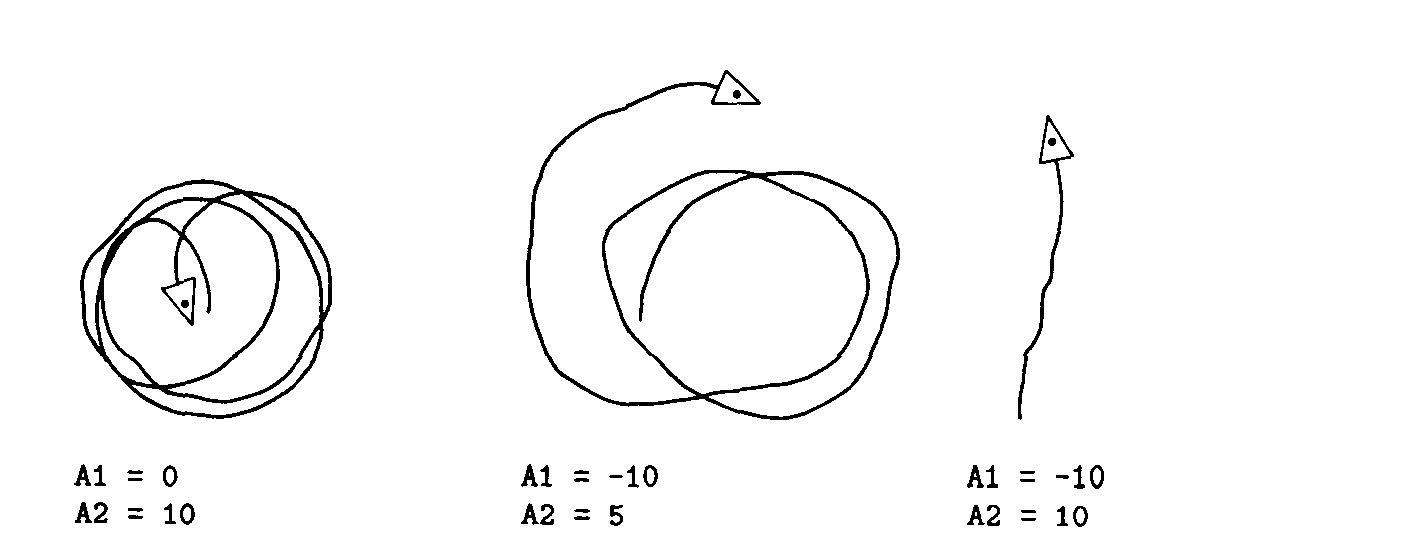
\includegraphics[scale=1]{fig2-1}
\caption{Sample paths generated by \textsc{random}\textsc{.move}}
\end{center}
\end{figure}

\subsection{Random Motion}

Perhaps the simplest kind of motion to model with the turtle is random
motion (repeatedly going forward and turning random amounts). To
implement this in a procedure, let's assume that our computer language
has a random-number generator \textsc{rand (low, high)} that outputs a random
number between \textsc{low} and \textsc{high}. Using this we can write a procedure that
takes four inputs specifying the ranges from which to select the inputs
to \textsc{forward} and \textsc{left}:

\begin{verbatim}
TO RANDOM.MOVE (D1, D2, A1, A2)
   REPEAT FOREVER
      LEFT RAND (A1, A2)
      FORWARD RAND (D1, D2)
\end{verbatim}
Even with this simple program, there is much to investigate. How do
the bounds on the \textsc{forward}s or the turns affect the path? For instance,
unless you make A1 negative the turtle will always turn left and the Y
path will look roughly like a circle. In fact, except when A1 is chosen to
be the negative of A2, the turtle's turning will be biased in one direction 
or the other and this will be reflected in the shape of the path. Figure
2.1 shows some examples. How about the case where the turning is 
unbiased? Would you expect the turtle to go off ``to infinity''? Or will 
it instead travel in a very large circle? More generally, can you say
anything about the radius of the ``average path'' as a function of the 
bounds on the turns? One way to investigate these random motions is to
write a record-keeping procedure that repeatedly runs, say, 100 rounds
of the \textsc{random.move} loop and automatically records such statistics as
the turtle's heading and distance from the origin after those 100 rounds.
Can you say anything about the average values of these quantities? (See
exercises 2 and 3.)

Random-motion procedures such as this will often run the turtle off
the edge of the display screen. Forcing the turtle to stay on the screen
suggests modifying the random motion to model the behavior of an
animal crawling in a box. To enable the turtle to do this, we'll supply
two new procedures: \textsc{check.forward}, which is just like \textsc{forward} except
that it won't allow the turtle to move if the result would take it outside of
some fixed square box around the origin, and \textsc{stuck}, which tells whether
or not the last move tried to place the turtle outside of the box.
The \textsc{checked.forward} program works by moving the turtle ``invisibly''
to the new position, then using a subprocedure \textsc{out.of.bounds}? to check
whether the new position is within bounds, and finally redoing the move
visibly only if it is within bounds. This procedure makes use of some
new operations in our turtle graphics system. \textsc{hideturtle} causes the
turtle indicator not to be displayed; \textsc{showturtle} restores the indicator;
\textsc{xcor} and \textsc{ycor} output, respectively, the $x$ and $y$ coordinates of the
turtle; \textsc{turtle.state} outputs (as a list) the position and heading of
the turtle; and \textsc{setturtle} takes as input a list such as is produced by
\textsc{turtle.state} and restores the turtle to that state:

\begin{verbatim}
TO CHECK.FORWARD DISTANCE
   OLD.POSITION <- TURTLE.STATE
   PENUP
   HIDETURTLE
   FORWARD DISTANCE
   FORWARD.FAILED <- OUT.OF.BOUNDS?
   SETTURTLE OLD.POSITION
   PENDOWN
   SHOWTURTLE
   IF NOT FORWARD.FAILED THEN FORWARD DISTANCE

TO STUCK
   RETURN FORWARD.FAILED

TO OUT.OF.BOUNDS?
   IF EITHER
         ABS (XCOR) > BOXSIZE
         ABS (YCOR) > BOXSIZE
      THEN RETURN "TRUE"
      ELSE RETURN "FALSE"
\end{verbatim}(\textsc{abs} is the absolute value function.)

\begin{figure}
\begin{center}
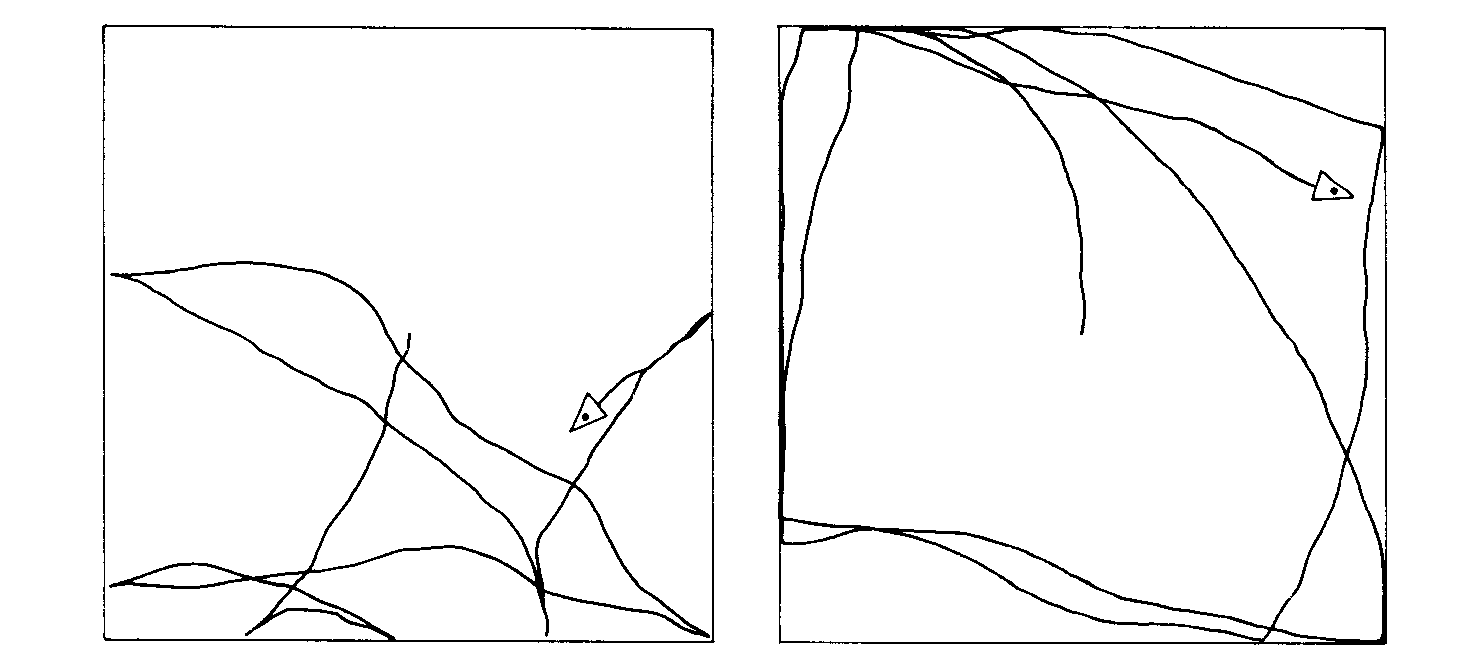
\includegraphics[scale=1]{fig2-2}
\caption{(a) Edge ``reflection'' generated by \textsc{if}\textsc{ stuck}\textsc{ then} \textsc{right} \textsc{180}. (b) Edge-following behavior generated by \textsc{if}\textsc{ stuck}\textsc{ then}\textsc{ wriggle}}
\end{center}
\end{figure}

We can use these procedures to model appropriate behaviors that
will keep the turtle in the box. Here, for example, is a version of
\textsc{random.move} that has the turtle turn $180^{\circ}$ whenever it runs into an
edge:

\begin{verbatim}
TO RANDOM.MOVE (D1, D2, A1, A2)
   REPEAT FOREVER
   LEFT RAND (A1. A2)
   CHECK.FORWARD RAND (D1, D2)
   IF STUCK THEN RIGHT 180
\end{verbatim}
shows a sample path. A second possibility for edge behavior
is to have the turtle turn a little at a time, until it can go forward again.
To do this, change the last line in the above procedure to \textsc{if}\textsc{ stuck}\textsc{ then}\textsc{ wriggle} where \textsc{wriggle} is defined as

\begin{verbatim}
TO WRIGGLE
   REPEAT
      RIGHT 1
      CHECK.FORWARD 1
   UNTIL NOT STUCK
\end{verbatim}
Figure 2.2b shows how this variation, incorporated into a random-motion
procedure, causes the turtle to spend most of its time wandering along
the edges of the box. You may have observed the similar behavior of
a real insect trapped in a box. Of course, with a real insect, this
behavior is often interpreted as the insect trying to get out of the
box by following the walls. The turtle program calls into question
the validity of such anthropomorphizing. If edge-following behavior
can be produced by a simple combination of random motion plus wall
avoidance, are we really justified in saying that the insect is ``trying'' to
follow the edge? Could we legitimately make this claim about the turtle?

\subsection{Directed Motion: Modeling Smell}

We can make our simulation more elaborate by allowing the turtle's
behavior to be affected by some stimulus. For example, we could imagine
that there is some food located in the box with the turtle and design
mechanisms that allow the turtle to find the food ``by sense of smell.''
There are many different ways we could provide turtles with information
corresponding to an ability to smell. For example, the ``amount of smell''
could be a value that depends on how far the turtle is from the food (the
larger the distance, the weaker the smell); or the turtle might not sense
any particular level of smell, but at each move be able to detect whether
the smell is getting stronger or weaker.

We'll begin with the second possibility. This ``stronger-weaker'' kind
of smell can be modeled by

\begin{verbatim}
TO SMELL
   IF DISTANCE.TO.FOOD > DISTANCE.LAST.TIME
      THEN RESULT <- "WEAKER"
      ELSE RESULT <- "STRONGER"
   DISTANCE.LAST.TIME <- DISTANCE . TO . FOOD
   RETURN RESULT
\end{verbatim}
How can the turtle use this information to locate the food? One possibility is this: If the turtle finds that the smell is getting stronger, it keeps going in the same direction; otherwise it turns:

\begin{verbatim}
TO FIND.BY.SMELL1
   REPEAT FOREVER
      FORWARD 1
      IF SMELL = "WEAKER" THEN RIGHT 1
\end{verbatim}
\begin{figure}
\begin{center}
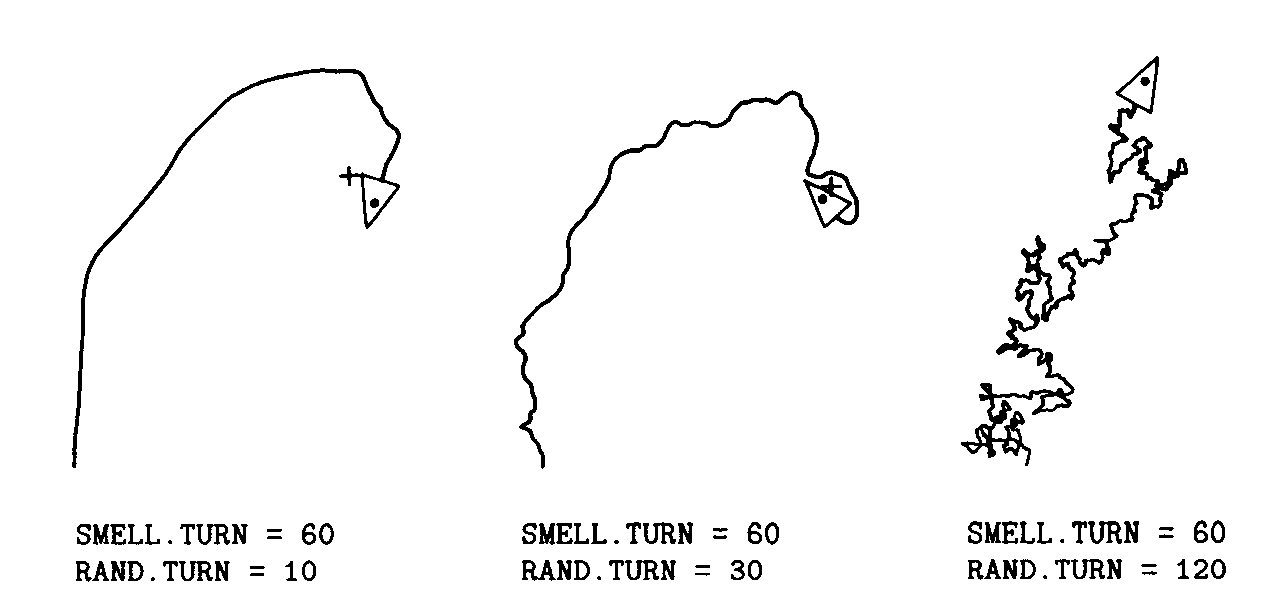
\includegraphics[scale=1]{fig2-4}
\caption{\textsc{find}\textsc{.by}\textsc{.smell3} illustrates degeneration of the algorithm under increasing randomness.}
\end{center}
\end{figure}

such intensity information to approach or avoid stimuli. Wood lice, for
example, are observed to aggregate in moist places and avoid dry places.
It is believed that they move in random directions, but that the moisture
level governs their speed-they move more slowly when it is damp and
hence spend most of their time in moist regions. This mechanism for
aggregation is called orthokinesis. A different mechanism, klinokinesis,
is claimed to govern the behavior of paramecia in aggregating in dark
areas. In klinokinesis, the animal's speed is constant, but the rate of
turning varies with the intensity of the stimulus. (For more information on these and other orientation mechanisms, see G. Fraenkel and
D. Gunn, Orientation in Animals [New York: Dover, 1961].) Try writing procedures embodying these mechanisms, and then try inventing
new mechanisms. Good questions to guide your exploration are: How
``efficient'' is your method (how long does it take the turtle to reach the
stimulus point)? How does the turtle's path change as you vary the initial position and heading, or as you vary the parameters to the program?
How does the mechanism degenerate as you incorporate some randomness into the turtle's motion (for example, as in the \textsc{find}\textsc{.by}\textsc{.smell3}
procedure above)? Will even a slight amount of randomness destroy the
turtle's ability to reach the goal, or is your mechanism relatively stable
with respect to random distortions?

In a more abstract vein, investigate the mathematical properties of
simple \textsc{poly}like programs, but think of some aspect of the turtle's motion
as governed by the distance from some chosen point. Try, for example,

\begin{figure}
\begin{center}
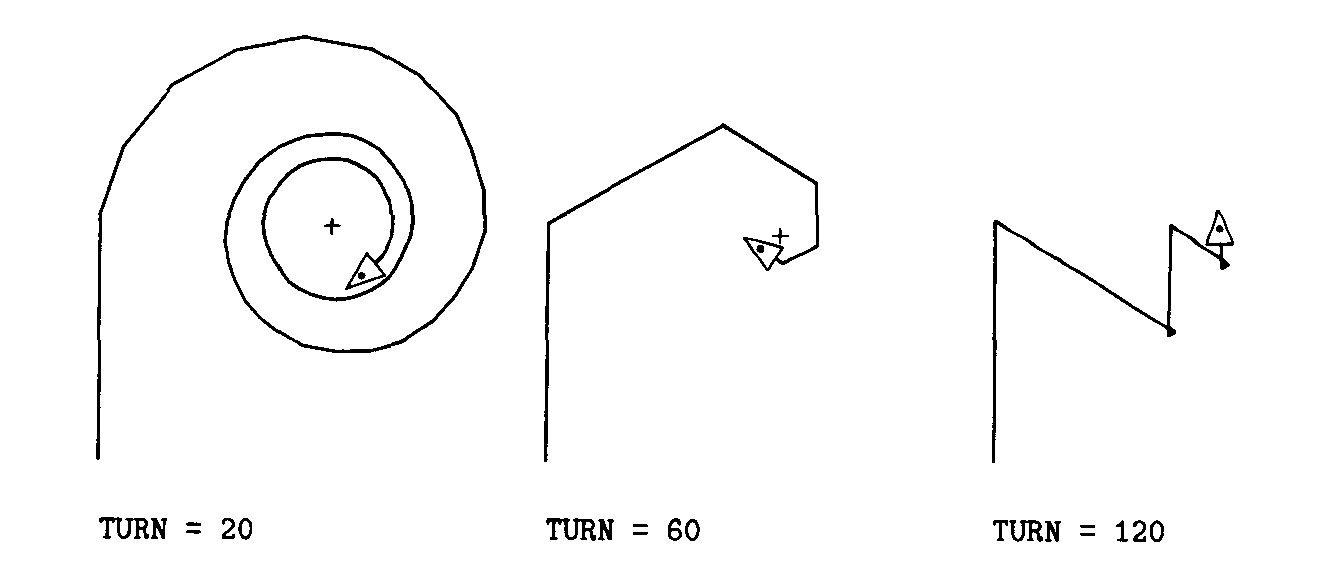
\includegraphics[scale=1]{fig2-3}
\caption{Paths generated by \textsc{find}\textsc{.by}\textsc{.smell2}}
\end{center}
\end{figure}

Experimenting further, we can add a parameter to adjust the size of the
turtle's turns. This leads to an interesting study of how the geometry
of the path varies with the turn angle. (See figure 2.3.)

\begin{verbatim}
TO FIND.BY.SMELL.2 (TURN)
   REPEAT FOREVER
      FORWARD 1
      IF SMELL = "WEAKER" THEN RIGHT TURN
\end{verbatim}
A more realistic simulation would also include some of` the random
motion of section 2.1.1:

\begin{verbatim}
TO FIND.BY.SMELL3 (D1, D2, SMELL.TURN, RAND.TURN)
   REPEAT FOREVER
      FORWARD RAND (D1, D2)
      LEFT RAND ( - RAND.TURN, RAND.TURN )
      IF SMELL = "WEAKER" THEN RIGHT SMELL.TURN
\end{verbatim}
In this procedure the turtle's motion is governed by two opposing tendencies: a ``random motion'' scaled by \textsc{rand.turn} and a ``directed motion'' scaled by \textsc{smell.turn}. This can be highlighted by adjusting the
relative sizes of the two parameters. As an experiment, see how large
\textsc{rand.turn} must be with respect to \textsc{smell.turn} before the random motion dominates completely and the turtle makes no discernible progress
towards the food. (See figure 2.4.)

A different possibility for sensing ``smell'' is to have the turtle respond
to an intensity directly, rather than to a change in intensity. Biologists
have suggested various simple mechanisms by which animals can use

\begin{figure}
\begin{center}
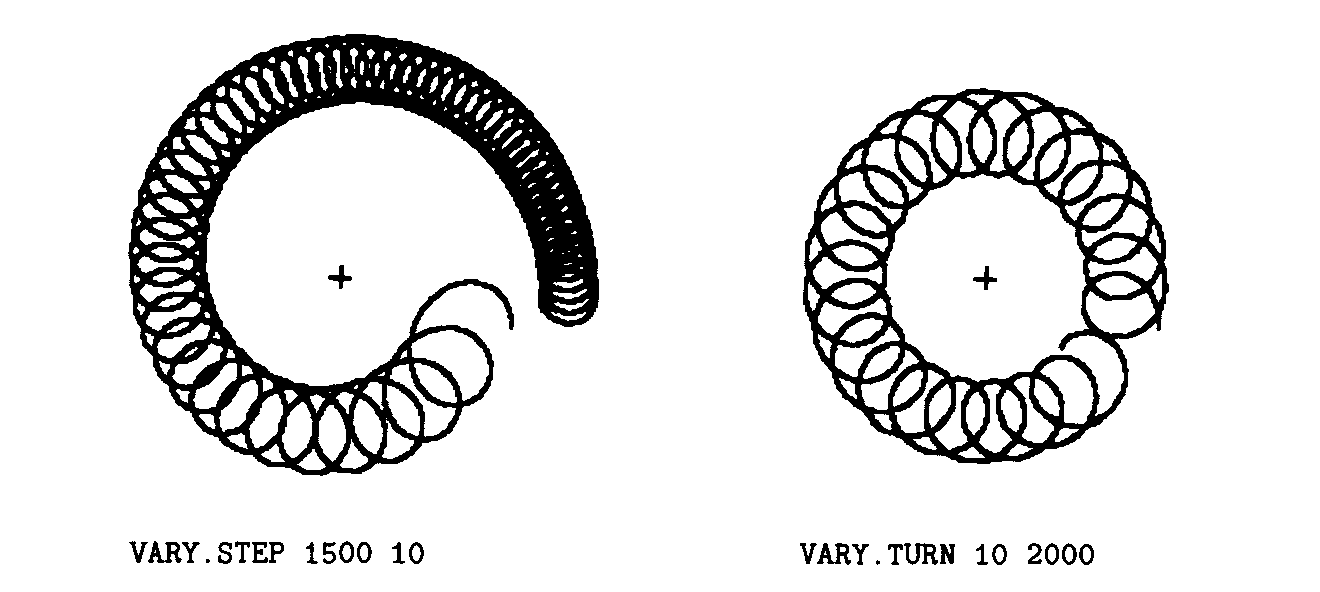
\includegraphics[scale=1]{fig2-5}
\caption{Samples of paths generated by \textsc{vary}\textsc{.step} and \textsc{vary}\textsc{.turn}.}
\end{center}
\end{figure}

having the turtle turn a constant angle while going forward a distance
that depends on the distance from the point:

\begin{verbatim}
TO VARY.STEP (SIDE, ANGLE)
   REPEAT FOREVER
      FORWARD (FACTOR * SIDE)
      LEFT ANGLE
\end{verbatim}
Or take a constant \textsc{forward} step and vary the turn:

\begin{verbatim}
TO VARY.TURN (SIDE, ANGLE)
   REPEAT FOREVER
      FORWARD SIDE
      LEFT (FACTOR * ANGLE)
\end{verbatim}
\textsc{factor} here can be something like

\begin{verbatim}
TO FACTOR
   RETURN (1 / DISTANCE.TO.CHOSEN.POINT)
\end{verbatim}
Figure 2.5 shows some sample paths. As you can see, the procedures
seem to do different sorts of things. \textsc{vary.step} tends to draw spirals,
whereas \textsc{vary.turn} tends to draw bounded figures. Investigate these
programs and come up with some conjectures about their behavior. Can
you prove your oonqectures?

\subsection{Modeling Sight}

As with smell, the first step in providing turtle with simulated sight is to
A decide what information the ``eye'' should receive from the environment.

\begin{figure}
\begin{center}
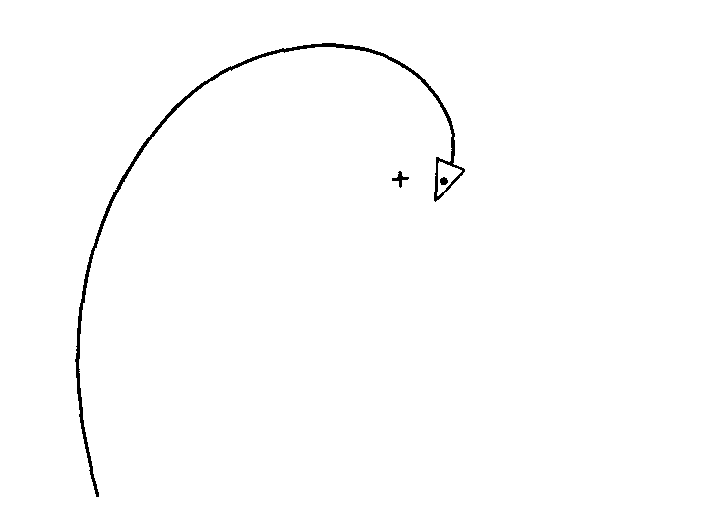
\includegraphics[scale=1]{fig2-6}
\caption{\textsc{keep.a.bearing}: \textsc{angle} = 60}
\end{center}
\end{figure}

We could hardly begin to model the complexity of human vision. A much
simpler model ignores color, shape, and texture and registers merely the
intensity of light reaching the eye. This kind of ``sight'' is not so different
from the ``smell'' discussed above. Each sense receives some kind of
intensity information from the environment. The major difference is
that sight is directional; it depends on how the turtle is facing with
respect to the stimulus. Algorithms for locating an object by sight are
therefore different from ``smelling something out.''

\subsubsection{Facing a Stimulus}

The first model for sight assumes that any creature able to see a light is
able to turn to face that light. (See exercise 10.) Investigate what new
things the turtle can do when given the ability to \textsc{face} a named point.
For example, getting to the point is easy: Simply face the point and go
forward. (But how does the turtle know when to stop?) Another use for
the \textsc{face} command is to have the turtle move while keeping some point
at a fixed bearing. The following procedure makes the turtle walk with
a fixed bearing of \textsc{angle} with respect to a fixed \textsc{point}:

\begin{verbatim}
TO KEEP.A.BEARING POINT ANGLE
   REPEAT FOREVER
      FACE POINT
      LEFT ANGLE
      FORWARD 1
\end{verbatim}

\begin{figure}
\begin{center}
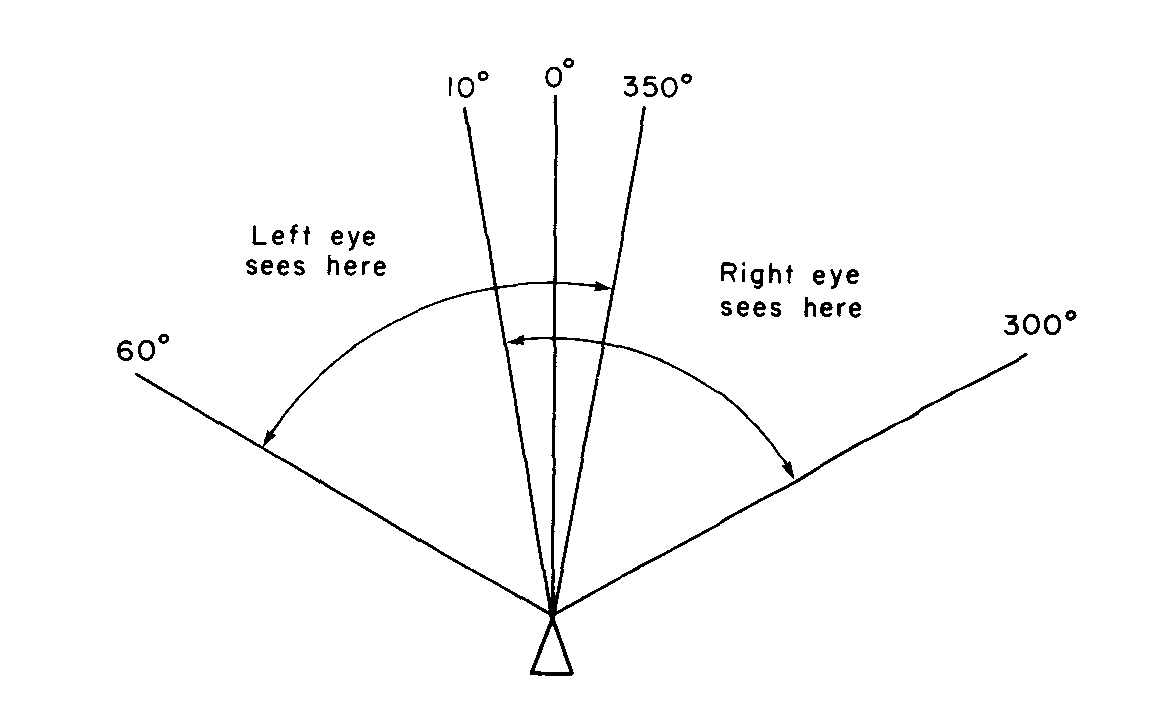
\includegraphics[scale=1]{fig2-7}
\caption{Fields of vision for two-eye model}
\end{center}
\end{figure}

If you try this procedure (figure 2.6) you will find that it causes the
turtle to spiral about the point. Does this remind you of anything? How
about a moth getting trapped by a light? Can you think of a reason
why a moth would be trying to keep a light at a fixed bearing? Some
people believe that moths and other night-flying insects have learned to
fly along straight paths by keeping the moon at a constant bearing as
they fly. Keeping a very distant light like the moon at a fixed bearing
would indeed make the insects fly straight. When they confuse the moon
with a nearby light, the fixed-bearing mechanism causes them to spiral.

\subsubsection{A Two-Eye Model}

The next model focuses on how a creature might use vision in order to
face a point. Assume that the turtle has two eyes, each with its own
tield of vision, as shown in figure 2.7. We give the turtle the ability to
tell whether a point is within each eye's field of vision:

\begin{verbatim}
TO RIGHT.EYE.SEES POINT
   IF BEARING (POINT) > 300 THEN RETURN "TRUE"
   IF BEARING (POINT) < 10 THEN RETURN "TRUE"
   RETURN "FALSE"

TO LEFT.EYE.SEES POINT
   IF BEARING (POINT) > 350 THEN RETURN "TRUE"
   IF BEARING (POINT) < 60 THEN RETURN "TRUE"
   RETURN "FALSE"
\end{verbatim}
\noindent (These procedures use a subprocedure called \textsc{bearing} that outputs the
angle that the turtle would need to turn left in order to face a given
point. Exercise 10 outlines how \textsc{bearing} can be implemented.)


\begin{figure}
\begin{center}
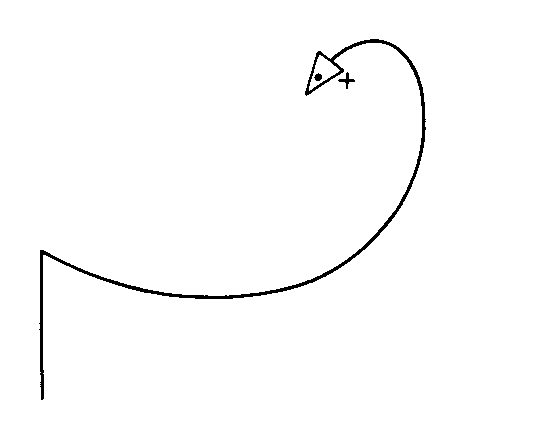
\includegraphics[scale=1]{fig2-8}
\caption{Behavior of \textsc{head}\textsc{.for}}
\end{center}
\end{figure}

The turtle will know that it is facing roughly in the direction of a
named point when the point lies in the field of vision on at least one
side. So, as the turtle moves, it should keep checking that it can still
see the point. Otherwise it turns until it can see the point:

\begin{verbatim}
TO HEAD.FOR POINT
   REPEAT FOREVER
      IF EITHER
         LEFT.EYE.SEES (POINT)
         RIGHT.EYE.SEES (POINT)
      THEN FORWARD 10
      ELSE LEFT 10
\end{verbatim}
It may seem amazing that a turtle following this procedure manages to
reach the specified point despite the fact that its way of heading for the
point is so inaccurate. (See figure 2.8.) This illustrates the effectiveness
of a feedback mechanism --- constant adjustment can often compensate
for lack of accuracy. You might try combining this mechanism with
some of the random-motion procedures of subsection 2.1.1.

\subsubsection{A Two-Eye Model With Intensity}

A more elaborate model for vision registers not only the presence of
a light source in the visual field, but also the intensity that each eye
receives from the source. This intensity depends on the strength of the
source, the distance of the source from the eye, and the angle at which
the light strikes the eye. The intensity is greatest when the light hits the
eye straight on and tapers off to zero as the light source moves toward
the edge of the visual field.

\begin{figure}
\begin{center}
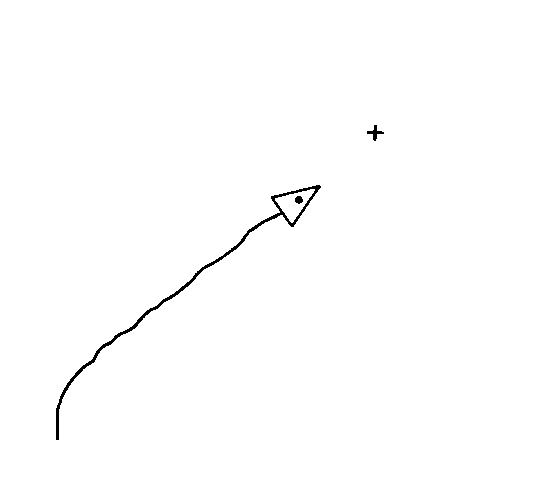
\includegraphics[scale=1]{fig2-9}
\caption{Path generated by \textsc{find}\textsc{.by}\textsc{.sight}}
\end{center}
\end{figure}

Suppose we have procedures \textsc{intensity.left} and \textsc{intensity.right}
that output the intensity each eye receives from a light source. (We'll
worry about how to design these \textsc{intensity} procedures later.) There is
a simple yet effective way to incorporate such intensity information in a
feedback mechanism to make the turtle approach the light source:

\begin{verbatim}
TO FIND.BY.SIGHT SOURCE
   REPEAT FOREVER
      FORWARD 1
      IF INTENSITY.LEFT (SOURCE) > INTENSITY.RIGHT (SOURCE)
      THEN LEFT 10
      ELSE RIGHT 10
\end{verbatim}
The turtle walks forward while trying to keep the amount of light
received at both eyes in balance. If the turtle sees more light to its
right, it turns slightly to the right. If it sees more light to its left, it
turns slightly to the left. (See figure 2.9.)

Some animals may actually use this mechanism for approaching light
sources. Biologists have obtained experimental evidence for this conclusion by taking an animal and masking one of its eyes. What happens
when the animal tries to approach the light? You can simulate this experiment by modifying \textsc{intensity.left} to always return 0 and have
the turtle follow the \textsc{find.by.sight} procedure. Now the turtle will always turn right, and will therefore travel in a circle. Biologists call this
behavior ``circus movement.'' It has been observed in experiments with
numerous species of insects.
A variation of this experiment is to modify \textsc{intensity.left} to output
half its normal value. (This corresponds to an animal with weak vision
in one eye.) What kind of path does \textsc{find.by.sight} produce now? Does
the animal still reach the light? How does the path degenerate to a circus
movement as the eye becomes weaker and weaker?

Finally, consider what happens when there are two or more light
sources. The intensity for each eye can be found by adding together
the intensities from the individual sources:

\begin{verbatim}
TO FIND.BY.SIGHT2 (SOURCE1, SOURCE2)
   REPEAT FOREVER
      FORWARD 1
      TOTAL.LEFT <- INTENSITY.LEFT (SOURCE1)
                       + INTENSITY.LEFT (SOURCE2) 
      TOTAL.RIGHT <- INTENSITY.RIGHT (SOURCE1)
                       + INTENSITY.RIGHT (SOURCE2)
      IF TOTAL.LEFT > TOTAL.RIGHT
      THEN LEFT 10
      ELSE RIGHT 10
\end{verbatim}
How does the turtle behave? Does it go to the stronger light? Between
the lights? Keep records of what happens for sources with different
strengths and for different initial positions of turtle and sources. This
``two-light experiment'' is often performed with real insects.
The intensity procedures used in these projects can be designed according to a model given in the book by Fraenkel and Gunn mentioned above.
They compute the intensity of light falling on the eye as $(S/D^2)\cos A$
where $S$ is the strength of the source, $D$ is the distance from the source,
and $A$ is the angle at which light from the source strikes the eye. (See
figure 2.10.) The turtle procedure based on this would be

\begin{verbatim}
TO INTENSITY.LEFT SOURCE
   IF NOT LEFT.EYE.SEES (SOURCE) THEN RETURN O
   FACTOR + STRENGTH / (DIST(SOURCE) | 2)
   ANGLE + BEARING (SOURCE) - 45
   RETURN (FACTOR * COS(ANGLE) 
\end{verbatim}
\noindent \textsc{strength} here is a parameter you supply to indicate the intensity of
the source. Note the computation of \textsc{angle}, which reflects the fact that
the left eye is offset $45^{\circ}$ from the turtle's heading. \textsc{intensity.right} is
implemented in a similar fashion.

\subsubsection{Exercises for Section \thesection}

\begin{figure}
\begin{center}
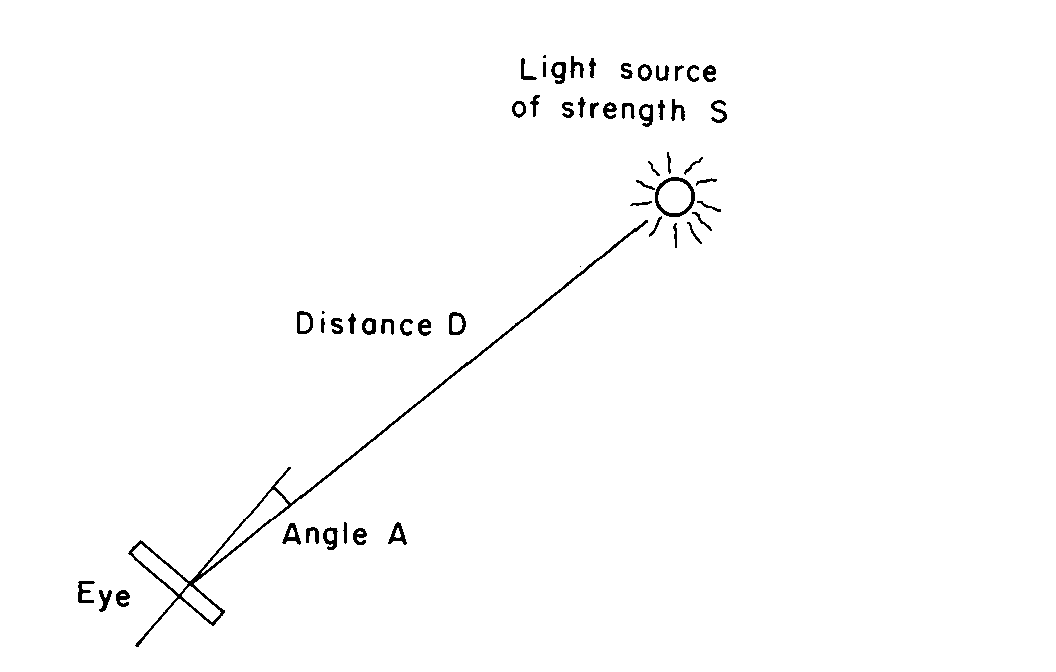
\includegraphics[scale=1]{fig2-10}
\caption{Intensity of light seen by eye is $(S / D^2) \cos A$.}
\end{center}
\end{figure}

\begin{enumerate}
\item $[P]$ In the \textsc{random.move} procedure of 2.1.1, how does the turtle's
path change if the turning is generated by \textsc{left rand(0, 50)} followed
by \textsc{right rand(0, 50)} rather than \textsc{left rand(-50,50)}? How is the
distribution of numbers produced by \textsc{rand(-50, 50)} different from that
of \textsc{rand(0, 50)} - \textsc{rand(0, 50)}? [A]
\item $[PD]$ Starting with the turtle facing straight up, run the \textsc{random.move}
procedure until the turtle exceeds distance n from the start, that is,
crosses a circle of radius $n$ centered at the starting point. At what point
did the turtle intersect the circle? Repeat this process over and over
and study the distribution of intersection points on the circle. What
is its ``average value''? How does the distribution change as $n$ varies?
Answer the same sort of questions about the number of steps taken
before crossing the circle.  
\item $[PDD]$ If the turtle follows \textsc{randommove} with the turn angle evenly 
distributed between -10 and 10, will you expect it to go off to infinity,
or to travel in a large circle? Make some studies of this phenomenon.
For example, graph the turtle's distance from the origin after n steps. ls
there an average graph for many tries of this experiment? Alternatively,
if the angle is not evenly distributed, the program will cause the turtle
to tend to walk in circles. But do the circles wander off to infinity? How
fast?
\item $[P]$ Investigate randomized \textsc{poly} procedures such as

\begin{verbatim}
TO RANDOM.POLY (SIDE, ANGLE)
   REPEAT FOREVER
      FORWARD SIDE
      LEFT (ANGLE * RAND (LOW, HIGH))
\end{verbatim}
\item $[P]$ In the \textsc{find.by.smell2} procedure of 2.1.2, how does the time
required to reach the food vary with the angle the turtle turns? In the
randomized \textsc{find.by.smell3} procedure, what is the average time as a
function of the \textsc{smell.turn} and \textsc{rand.turn}? (Do some experiments and
take statistics.)
\item $[P]$ Implement procedures for orthokinesis and klinokinesis. Which is
more efficient? Which is more stable under adding a bit of randomness?
Does the stability depend on the kind of randomness?
\item $[P]$ Play around with the \textsc{vary.step} procedure of 2.1.2. Does the
turtle always spiral inwards or outwards? Does this depend on the initial
position or heading with respect to the fixed point? Try also taking
different values for \textsc{factor}, such as making it directly proportional to
the distance from the point or inversely proportional to the distance
squared.
\item $[P]$ What can you say about the \textsc{vary.turn} procedure? Does the
turtle always stay within a bounded distance from the fixed point? Try
this also with the variations on \textsc{factor}, as in exercise 7.
\item $[P]$ Try procedures like \textsc{vary.step} and \textsc{vary.turn}, only this time
where \textsc{factor} depends on the change in distance (as with the \textsc{smell}
procedure of 2.1.1). For instance, suppose \textsc{factor} is equal to \textsc{distance} $-$
\textsc{distance.last.time}. Consider the procedure

\begin{verbatim}
REPEAT FOREVER
   FORWARD SIDE
   LEFT FACTOR
\end{verbatim}
\noindent Prove that this can never draw a simple closed figure. [HA]

\item $[P]$ Implement the \textsc{face} and \textsc{bearing} procedures used in the sight
programs of 2.1.3. \textsc{bearing} should return the amount the turtle needs to
turn left in order to face the point. Then \textsc{face} can be immediately implemented as \textsc{left (bearing (point))}. \textsc{bearing}, in turn, can be implemented in terms of the turtle's heading and another function, \textsc{towards},
which outputs the heading of the line directed from the turtle to the
point. This can be computed using an arctangent function. [A]
\item $[P]$ Make a careful investigation of the two- (or more) light experiment. How does the turtle's path vary with the relative intensities of
the light?
\item $[P]$ Suppose the turtle lives in a square room with a light at each
corner. Instead of using a rectangular coordinate system, the turtle can
``get its bearings'' by measuring the observed angles between the lights.
Suppose the turtle starts at some point $p$ and records the observed
angles. Now move the turtle to a different point. Design a simple
feedback algorithm that enables the turtle to return to $p$ by moving
and watching how the angles change.
\end{enumerate}

\section {Turtles Interacting}

One natural extension of the previous section's ``turtle biology'' is to
consider multiple turtles and the interactions produced by simple algorithms. As we shall see, even simple algorithms may lead to complex
phenomena, and a study of these phenomena can be an invitation to the
theory of ``differential games.''

\subsection{Predator and Prey}

Consider how the \textsc{find.by.smell} mechanism of subsection 2.1.2 would
behave if the food were also moving, as in the case of a predator trying
to catch dinner. There are many possible variations to try. Suppose, for
example, that the hunted creature, unaware of the predator's intentions,
moves round and round in a circle and that the predator follows the
prey according to the \textsc{find.by.smell2} procedure of 2.1.2. One way to
implement this interaction is to write separate procedures for predator
and prey that describe how each creature generates a single forward
step:

\begin{verbatim}
TO PREY.STEP (SPEED, TURN)
   FORWARD SPEED
   RIGHT TURN

TO PREDATOR.STEP (SPEED, TURN)
   FORWARD SPEED
   IF SMELL = "WEAKER" THEN RIGHT TURN
\end{verbatim}
Now supply a monitor procedure called \textsc{execute.together} that executes these two procedures alternately, over and over;

\begin{verbatim}
TO EXECUTE.TOGETHER (PREDATOR.PROCESS, PREY.PROCESS)
   REPEAT FOREVER
   ; set the turtle at the predator state and
   ; execute the predator's procedure
      EXECUTE.STEP (PREDATOR.PROCESS, PREDATOR.STATE)
      ; save the predator state for next time
      PREDATOR.STATE <- TURTLE.STATE
      ; execute the prey's procedure
      EXECUTE.STEP (PREY.PROCESS, PREY.STATE)
      ;save the prey state
      PREY.STATE <- TURTLE.STATE
\end{verbatim}
The inputs to this procedure are to be the \textsc{step}s above, with their inputs.
For instance,

\textsc{execute.together(``prey.step(1,1)'' . ``predator.step(2,90)'')} 
makes the prey and predator execute simultaneously.

The \textsc{execute.step} procedure is responsible for executing the process
in the right place. It makes the turtle follow a given process starting
from a given state.

\begin{verbatim}
TO EXECUTE.STEP (PROCESS, STATE)
   ; with the pen up move the turtle to the starting state
   PENUP
   SETTURTLE STATE
   ; put the pen down and execute the process
   PENDOWN
   EXECUTE PROCESS
\end{verbatim}
At any point during the process, the variables \textsc{predator.state} and
\textsc{prey.state} specify the position and heading of the creatures. Set
these to their initial values before starting the \textsc{execute.together} procedure. (Note: Some computer languages have built-in facilities for parallel
processing, which eliminate the need for such a \textsc{execute.together} procedure. But since these languages are not yet widespread, we show how
to implement this in a more conventional language. Also, see appendix
A for details about the \textsc{execute} command.)

\begin{figure}
\begin{center}
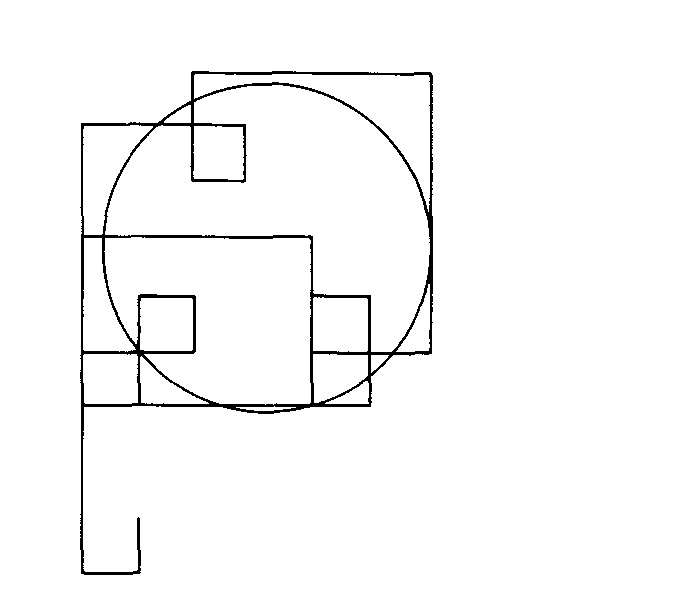
\includegraphics[scale=1]{fig2-11}
\caption{Closed-path phenomenon. Predator uses \textsc{find}\textsc{.by}\textsc{.smell} with \textsc{turn} = 90; prey moves in circle. Predator speed is twice prey speed}
\end{center}
\end{figure}

Figure 2.11 shows the result of the two procedures with the predator's
\textsc{turn} equal to $90^{\circ}$ and with predator moving twice as fast as prey. As
you can see, the \textsc{find.by.smell} mechanism, which works so well with
a fixed food source, does very poorly when the food is moving. The
geometry of the path, however, is interesting. Notice that, after an initial
segment, the predator's path is closed. Can you see why? Investigate this
phenomenon for different \textsc{turn} angles in the \textsc{predator}\textsc{.step} procedure
and also for varying relative speeds of predator and prey.
Now conduct a similar investigation with some of the other animal-orientation mechanisms of section 2.1. Do they all do so poorly when
the food is moving? Or consider the use of these simple algorithms
as avoidance mechanisms. For example, set up a situation in which
A a predator uses one of the sight algorithms of 2.1.3 to chase another
creature that is using an \textsc{avoid}\textsc{.by}\textsc{.smell} procedure. (Note: To convert
\textsc{find}\textsc{.by}\textsc{.smell} to \textsc{avoid}\textsc{.by}\textsc{.smell}, simply modify the procedure so
that the creature will turn whenever the smell is getting stronger.) Any
such combination of the behaviors illustrated in section 2.1 can serve as
the basis for a project.

\subsection{Following and Chasing}

In a slightly different framework, we can consider ``chase and evade''
strategies for two turtles. The simplest strategy is for the chasing turtle
to run directly towards the evader, and for the evader to run directly
away from the chaser. More interesting is the situation when both
creatures are constrained to stay within a square box. There are lots
of possibilities for projects here. Begin by programing simple strategies
using the \textsc{execute}\textsc{.together} framework of 2.2.1. Now make the chaser
a bit smarter so that he can generally catch the evader --- for example, by
driving him into a corner. Now make the evader smarter, so that he can
avoid the trap. Now make the chaser smarter still, and so on. When you
get some really clever programs, modify the setup so that you control
one of the creatures by hand and the computer controls the other. Are
your clever procedures more skilled at the chase-evade game than you
are? As a test of skill and strategy, try varying the relative speeds of
chaser and evader. If they both move at the same speed, can the evader
always avoid being caught?

\begin{figure}
\begin{center}
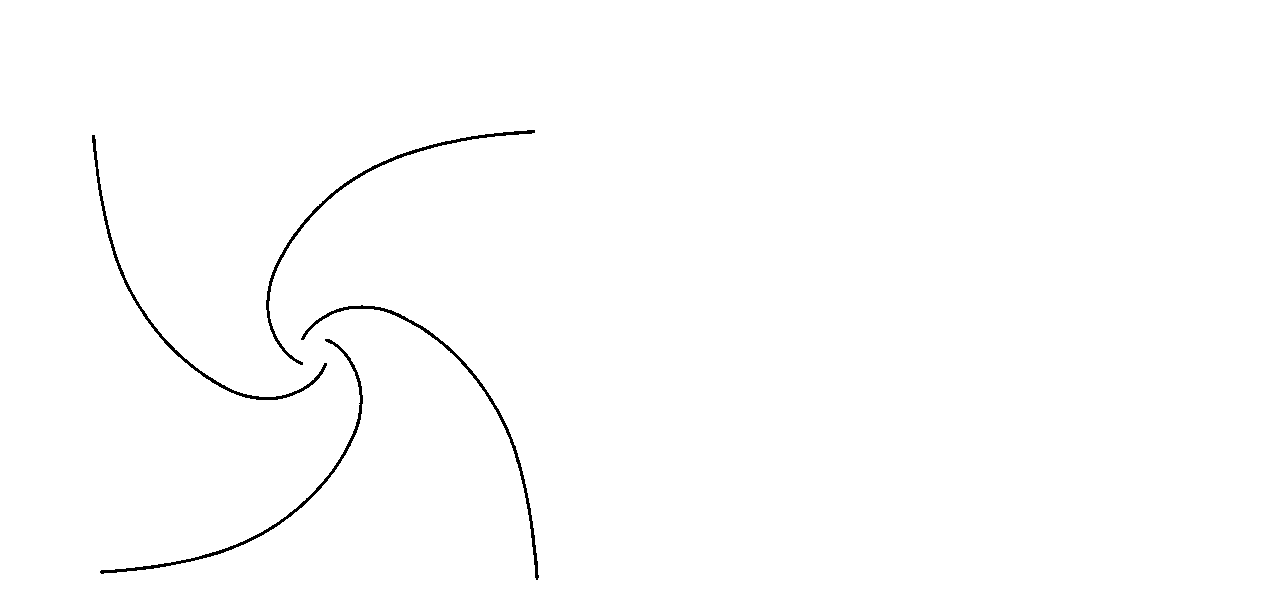
\includegraphics[scale=1]{fig2-12}
\caption{Spiral paths generated by four ``bugs'' starting at vertices of square.}
\end{center}
\end{figure}

It's also interesting to examine the paths generated by interacting
creatures. One example is the widely known mathematical problem
of the four ``bugs'' who start at the vertices of a square and move at
the same speed, each one following the bug to its right. Set this up
using the \textsc{execute.together} procedure (suitably modified to handle
four creatures) and the \textsc{follow} mechanism:

\begin{verbatim}
TO FOLLOW.THAT.BUG
   FACE THAT.BUG
   FORWARD 1
\end{verbatim}
Now make bug 1 follow bug 2, bug 2 follow bug 3, bug 3 follow bug 4,
and bug 4 follow bug 1:

\begin{verbatim}
EXECUTE.TOGETHER "FOLLOW BUG2" "FOLLOW BUG3" 
            "FOLLOW BUG4" "FOLLOW BUG1"
\end{verbatim}
Figure 2.12 shows the paths generated by the four bugs. As you can
see, they all meet at a single point. One notable property of the ``four
bugs'' situation is that the length of the path traveled by each bug is
equal to the side of the original square. See if you can prove that.
Modify \textsc{follow} to keep track of how far each bug moves, and compare
the computed value with the theoretical value.
Here is another interesting chase phenomenon with two creatures, the
chaser and the evader. The chaser heads directly towards the evader:

\begin{figure}
\begin{center}
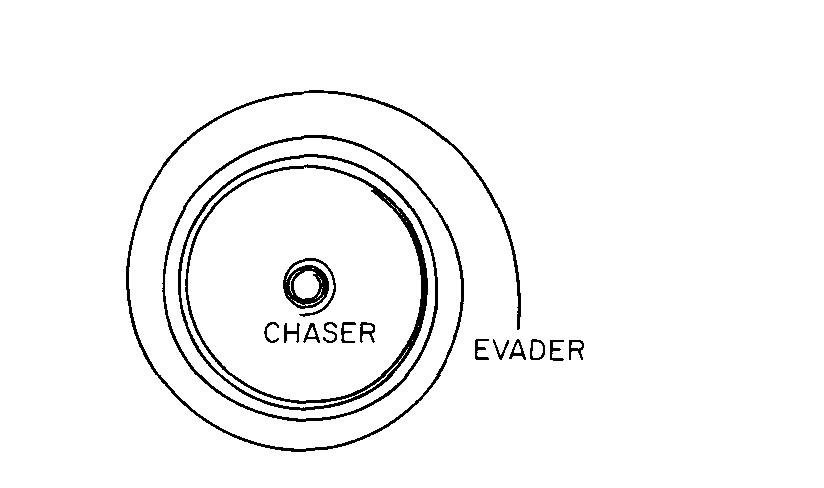
\includegraphics[scale=1]{fig2-13}
\caption{Stable configuration generated by interaction of \textsc{chase} and \textsc{evade}}
\end{center}
\end{figure}

But the evader, instead of running directly away, heads at a constant $90^{\circ}$ bearing from the chaser:


\begin{verbatim}
TO CHASE
   FACE EVADER
   FORWARD CHASE.SPEED

TO EVADE
   FACE CHASER
   RIGHT 90
   FORWARD EVADE.SPEED
\end{verbatim}
When the two creatures move at the same speed, the chaser always
catches up, as you might expect. But when the evader's speed is increased, both chaser and evader begin to spiral in towards each other.
The spirals eventually degenerate into closed circles (see figure 2.13),
which are stable configurations for the chaser-evader situation. Even
though the algorithm seems ``directed,'' the creatures end up retracing
their paths over and over.

A multiple-turtle setup can also be used to investigate some of the
phenomena in the area of ``differential games,'' which has to do with
finding optimal strategies in situations similar to ``chase and evade.'' An
example is provided by a ``target defending'' game consisting of two
players and a target. The attacker's object is to get as close to the
target as possible; the defender's object is to intercept the first player as
far from the target as possible. Assume that both players have the same
speed and that the defender starts out closer to the target. It turns out
that this situation has a simple optimal strategy, which is the same for
both players: Each time you move, head for the point that is closest to
the target and that lies on the perpendicular bisector of the line joining
your position to your opponent's (see exercise 11). Of course, if both
players are computerized and move with optimal strategy (figure 2.14a)
the resulting paths aren't very interesting-a better idea might be to
arrange things so that you control one player and the computer controls

\begin{figure}
\begin{center}
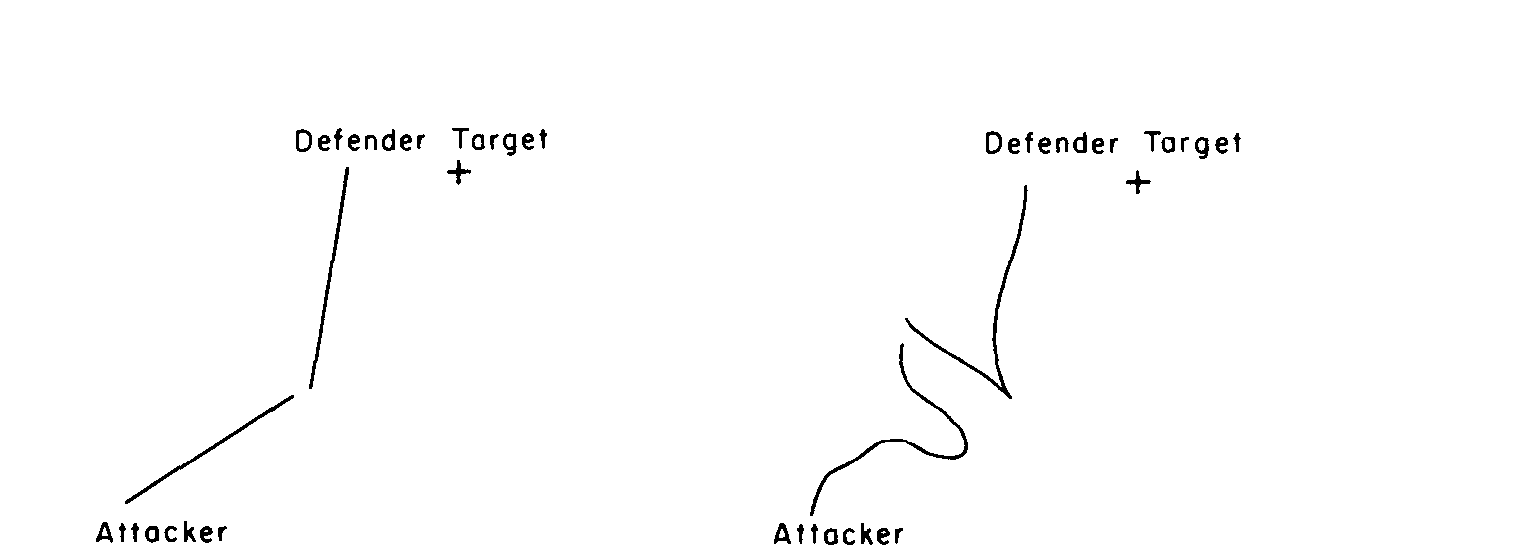
\includegraphics[scale=1]{fig2-14}
\caption{Targetrdefending game. (a) Both players following optimal strategy. (b) Attacker manually controlled; defender computer-controlled following optimal strategy. the other (see figure 2.14b). Try playing against the computer both on attack and on defense. How well can you do in comparison with the theoretical optimum?}
\end{center}
\end{figure}

Books on differential games suggest many more situations that can be
made into games between a person and a computer. In general these
are very difficult to analyze for optimal strategies; the target-defending
game explained above is unusually straightforward. There is a Way to
simplify the situation: Restrict all creatures to move on a square grid;
that is, only allow turns that are multiples of 900 and distances that
are multiples of some fixed length, or, alternatively, specify that at each
step a creature can move only to an adjacent square in the grid.

\subsubsection{Exercises for Section \thesection}
\begin{enumerate}
\item $[PD]$ Can you verify, as asserted in subsection 2.2.1, that a predator
using \textsc{find}\textsc{.by}\textsc{.smell} to chase a creature moving in a circle will eventually travel in a closed path? How does this depend on the angle turned?
On the relative speeds of predator and prey? On the initial positions?
\item $[P]$ Set up a predator using \textsc{find}\textsc{.by}\textsc{.sight} (subsection 2.1.3) to chase
a prey using \textsc{avoid}\textsc{.by}\textsc{.smell}. Does he catch him if the two creatures
have equal speeds? Does this depend on the angles that the creatures
turn? What happens as the speeds vary?
\item $[P]$ Implement a general \textsc{execute}\textsc{.together} facility that can handle,
say, two, three, or four creatures simultaneously. Notice that the procedure given in the text draws only the creatures' paths and not the
creatures themselves. Maybe you'd like to improve upon this.
\item $[P]$ Implement a general ``chase-evade'' system that allows you to
specify procedures to guide both chaser and evader, or to control either
creature by hand.
\item $[PD]$ Set up the ``four bugs'' simulation. Have the system calculate
the distance traveled by each bug. Does your result agree with the claim
in the text that this distance is equal to the side of the original square?
Can you prove this claim?
\item $[PDD]$ Suppose that, instead of four bugs, we have three bugs starting
in the vertices of an equilateral triangle. How far does each bug travel
now? Generalize this to consider $n$ bugs starting at the vertices of a
regular n-gon. Given a formula for the distance traveled by each bug in
terms of the side of the $n$-gon, and check your formula by doing some
computer simulations. [A]
\item $[P]$ Make up and investigate some variations on the ``four bugs''
problem. For example: Suppose the bugs start on a figure that is not so
symmetric. (How about a rectangle?) Suppose one bug goes faster than
the other. Suppose instead of each bug following the one to its left, they
follow each other in some other order.
\item $[P] $What kinds of initial conditions, speeds, and following mechanisms
will ensure that all bugs eventually meet at one point?
\item $[PD]$ Investigate the modified chase-evade simulation that yields the
stable circles of 2.2.2, assuming that the evader movers faster than the
chaser. Why does the process stabilize? When it does stabilize, what is
the approximate distance of chaser from evader? How does this distance
depend on the speeds of chaser and evader? Give a formula for the
distance.  
\item $[P]$ Find other chase-evade pairs that produce stable configurations.
\item In the ``target-defending'' game, give a formula for the coordinates
of the point to head for when following the optimal strategy, and use
this to implement the strategy on the computer.  
\item $[D]$ Analyze the target-defending game in the case where the two
players have different speeds. What is the optimal strategy for each
player?  
\item $[P]$ Carry out a detailed study of chase-evade for creatures moving on
a grid. Invent strategies and counterstrategies. Can the evader always
avoid getting caught if the two creatures move at equal speeds? If they
move at different speeds?
\end{enumerate}

\begin{figure}
\begin{center}
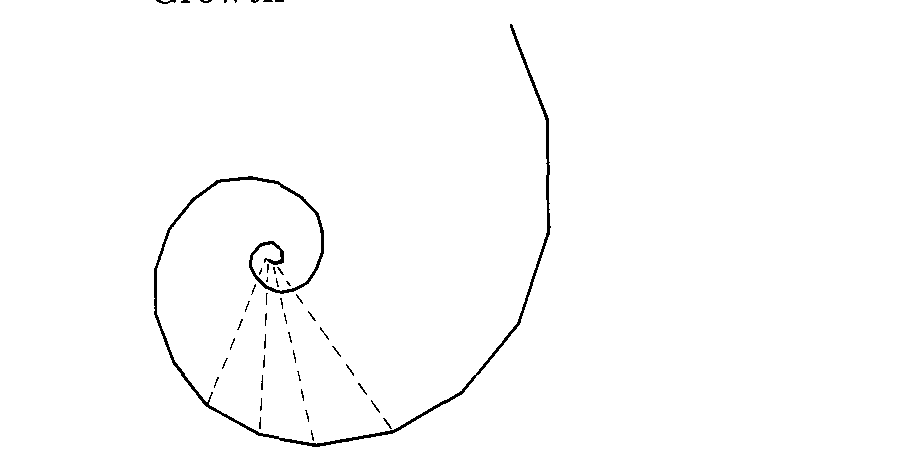
\includegraphics[scale=1]{fig2-15}
\caption{Equiangular spiral formed by \textsc{eqspi} with \textsc{angle} = 20, \textsc{scale} = 1.1.}
\end{center}
\end{figure}

\section{Growth}

Besides simulating animal behavior, another good source of turtle biology projects is modeling patterns of growth. In this section we'll examine
two models: the equiangular spiral, which emerges in the shapes of shells
and horns; and models for branching in the growth of trees.

\subsection{Equiangular Spirals}

We've already seen in section 1.1 how to transform the \textsc{poly} program

\begin{verbatim}
TO POLY SIDE ANGLE
   FORWARD SIDE
   LEFT ANGLE
   POLY SIDE ANGLE
\end{verbatim}
\noindent into a program for drawing spirals:

\begin{verbatim}
TO POLYSPI (SIDE, ANGLE, INCREMENT)
   FORWARD SIDE
   LEFT ANGLE
   POLYSPI (SIDE + INCREMENT, ANGL, INCREMENT)
\end{verbatim}
Here is another way to make a spiral: Rather than increasing the side by
adding a fixed increment, multiply the side by a constant scale factor:

\begin{verbatim}
TO EQSPI (SIDE, ANGLE, SCALE)
   FORWARD SIDE
   LEFT ANGLE
   EQSPI (SIDE * SCALE, ANGLE, SCALE)
\end{verbatim}
This spiral (shown in figure 2.15) is called aniequiangular spiral (also
sometimes called a logarithmic spiral). Connecting the vertices of the
spiral to a central point shows that the spiral can be generated by 
successions of similar triangles, each one built upon the previous. This
principle of constructing a pattern through the accumulation of similar
shapes lies behind the spiral's appearance in many biological forms,
especially in shells and horns. The nautilus shell, shown in figure 2.16,
gives a clear illustration. The entire shell is constructed as a sequence of
``chambers,'' each chamber built on the previous chamber and similar to
it. (The chambers are similar because the creature doesn't change shape
as it moves from chamber to chamber; it just grows.) The result is that
corresponding points of successive chambers lie on equiangular spirals.
We'll exhibit a turtle program that mimics this kind of equiangular
growth, using quadrilateral chambers. Each quadrilateral, as indicated
in figure 2.17a, will be specified to the program by three sides and two
angles. If the turtle starts in the lower left corner, the base and sides of
the quadrilateral can be drawn by

\begin{verbatim}
TO CHAMBER (BASE, S1, S2, A1, A2)
; save the position of the lower left vertex
   LOWER.LEFT + TURTLE.STATE
   ; draw the base and right side and save the
   ; position of the upper right vertex (see below)
   FORWARD BASE
   LEFT A2
   FORWARD S2
   UPPER.RIGHT + TURTLE.STATE
   ; return to the lower left vertex and draw the left side
   PENUP
   SETTURTLE LOWER.LEFT
   PENDOWN
   LEFT A1
   FORWARD S1
\end{verbatim}

\begin{figure}
\begin{center}
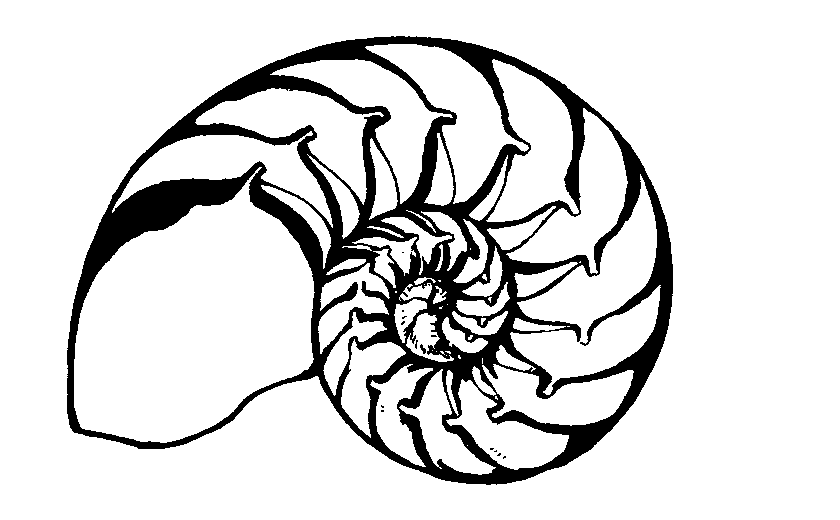
\includegraphics[scale=1]{fig2-16}
\caption{The shell of the chambered nautilus clearly exhibits the spiral-growth phenomenon.}
\end{center}
\end{figure}

\begin{figure}
\begin{center}
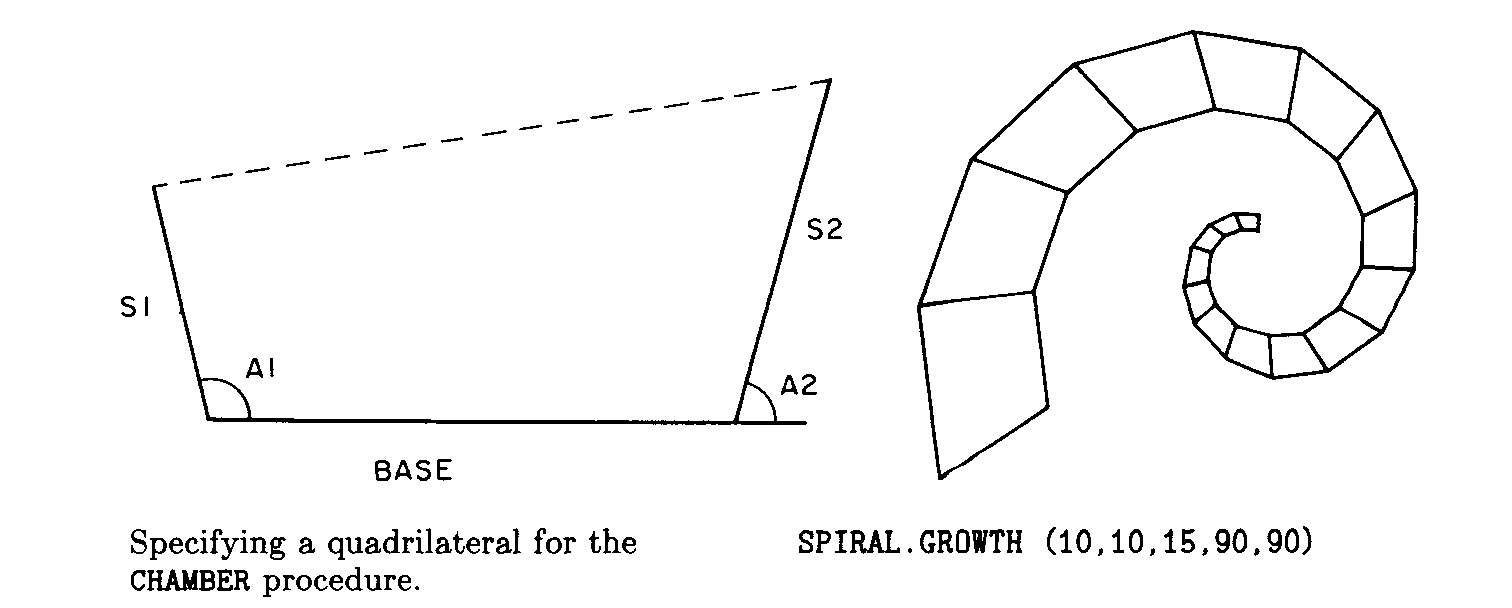
\includegraphics[scale=1]{fig2-17}
\caption{The \textsc{spiral}\textsc{.grow} procedure.}
\end{center}
\end{figure}

At the end of this procedure the turtle is sitting at the upper left corner
1 of the chamber, which is the same as the lower left vertex of the next
chamber. To prepare for drawing the next chamber we must point the
turtle along the base of the next chamber, that is, point the turtle
towards the upper right vertex of the chamber just drawn. We can do
this using the \textsc{face} procedure of section 2.1, whose implementation is
outlined in exercise 10 of that section. Having done this, we are ready
to draw the next chamber. The angles of the next chamber are the same
as before. The base of the next chamber is the top edge of the previous
chamber, and the size of the next chamber is determined by the ratio
of the old base to the new base. All together, the program for spiral
growth is

\begin{verbatim}
TO SPIRALGROWTH (BASE, S1, S2, A1, A2)
; draw one chamber and face along the edge of the new chamber
   CHAMBER (BASE, S1, S2, A1, A2)
   FACE UPPER.RIGHT
   ; the length of the next chamber's base is the distance
   ; from the current location to the upper right corner of
   ; the chamber just drawn
   NEXT.BASE <- DISTANCE (UPPER.RIGHT)
   ; compute the ratio of the sides of the new chamber to the
   ; sides of the previous chamber
   R <- NEXT.BASE/BASE
   ; now repeat the process, using as inputs
   ; the sides and angles of the new chamber
   SPIRAL.GROWTH (NEXT.BASE, S1 * R, S2 * R, A1, A2)
\end{verbatim}
\begin{figure}
\begin{center}
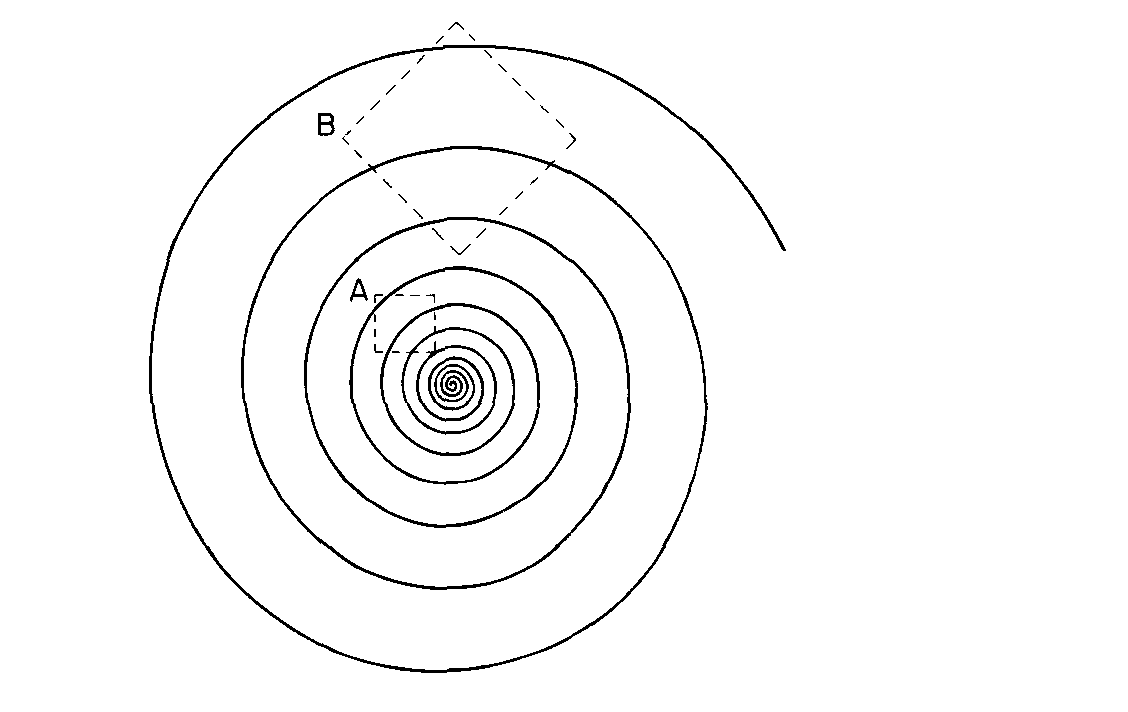
\includegraphics[scale=1]{fig2-18}
\caption{Demonstration that curves of equiangular spiral are everywhere the same. Chunk B is the same as chunk A blown up by a factor of 3}
\end{center}
\end{figure}

The recursive structure of the program implies that each chamber generates
a new chamber. There is no stop rule and the program goes on forever.
Whether the chambers increase or decrease in size depends on the initial
sides and angles. A sample ``shell'' drawn by this program is illustrated in
figure 2.17.

\subsubsection{Growing Turtle Geometry}

Equiangular spirals underlie uniform growth such as the \textsc{spiral.growth}
shown above in the same way that a circle underlies any turtle program
that does the same thing over and over. The reason for both of these
facts becomes clearer when one describes the equiangular spiral and the
circle as curves that are ``everywhere the same.'' In the case of a circle,
that means any chunk of the circle can match any other chunk of the
circle if you are allowed to move and turn the iirst chunk. In the case
of the spiral, one must allow changing scale (making a bigger or smaller
model of a piece), in addition to moving and turning, to show that one
piece matches another. See figure 2.18.

One can augment turtle geometry to make scale changes by introducing a new ``scaled forward'' command and a \textsc{grow} command to change
scale:

\begin{verbatim}
TO S.FORWARD DISTANCE
   FORWARD (SCALE * DISTANCE)
 
TO GROW FACTOR
   SCALE <- (SCALE * FACTOR)
\end{verbatim}
\noindent \textsc{scale} should now be considered a part of the turtle state --- it's a kind
of ``size'' of the turtle that determines the size of the next step just as
heading determines the direction of the next step. (\textsc{scale} should start
equal to 1.)
The analog to \textsc{poly} is precisely \textsc{eqspi}:

\begin{verbatim}
TO EQSPI (SIZE, ANGLE, FACTOR)
   REPEAT FOREVER
      S.FORWARD SIZE
      RIGHT ANGLE
      GROW FACTOR
\end{verbatim}
You should be able to show that any looping program which involves
only \textsc{s.forward}, \textsc{right}, and \textsc{grow} will have an \textsc{eqspi} skeleton, just as
\textsc{poly} is the skeleton for looping programs without \textsc{grow} (see exercise
10). Incidentally, a circle is an ``equiangular spiral with no growth'' in
the same way a line is ``a circle with no turning.'' Finally, notice that
the chambered growth shown in figure 2.17 ensures that the growth is
uniform by having the bottom edge of one chamber be related to the
bottom edge of the preceding precisely as the ratio of top to bottom
edge of the previous chamber. Because the chambers are constructed to
be similar, that ratio never changes.

\subsection{Branching Processes: A Lesson in Recursion}

A different kind of growth pattern we can mimic with turtle graphics
is the branching process that characterizes the growth of trees. We'll
start by drawing a very regular binary tree, that is, a tree in which
each branch sprouts two more branches. We'll make the length of each
sprouted branch half that of the parent. Conceptually, each branch
consists of a straight line, with two more branches at its end. Notice the
fundamentally recursive nature of this description --- a branch consists of
something (the stem) plus sub-branches (things with the same structure
as the branch). In a program, that structure will appear in the standard
recursive way, as a procedure calling itself as a subprocedure.

If we assume that the branching angle is $45^{\circ}$, then a first try at a
program might be

\begin{verbatim}
TO BRANCH LENGTH
; draw the main branch
   FORWARD LENGTH
   ; turn to point along the left
   ; secondary branch and draw it
   LEFT 45
   BRANCH LENGTH / 2
   ; now draw the right secondary branch
   RIGHT 90
   BRANCH LENGTH / 2
\end{verbatim}
But if we try this procedure, we'll find that it has a bug: The turtle starts
drawing a branch, then its left secondary branch, then that branch's
left secondary branch, and so on and so on. No right branches ever get
drawn. At some point, we must make the process stop generating new
left branches and come back to do the right branches. We'll accomplish
this by giving the \textsc{branch} process a second input called \textsc{level}, which
counts down as the program moves from each branch to its secondary.
We can think of \textsc{level} as labeling the type (complexity) of the branch:
A level 1 branch is a tip (a branch with no secondaries); a level 2 branch
will sprout two level 1 secondaries; a level 3 branch will sprout level 2
secondaries, and so on. The program should stop generating secondary
branches whenever the level reaches 0:

\begin{verbatim}
TO BRANCH (LENGTH, LEVEL)
   IF LEVEL = 0 THEN RETURN
   FORWARD LENGTH
   LEFT 45
   BRANCH (LENGTH/2, LEVEL - 1)
   RIGHT 90
   BRANCH (LENGTH/2. LEVEL · 1)
\end{verbatim}
\begin{figure}
\begin{center}
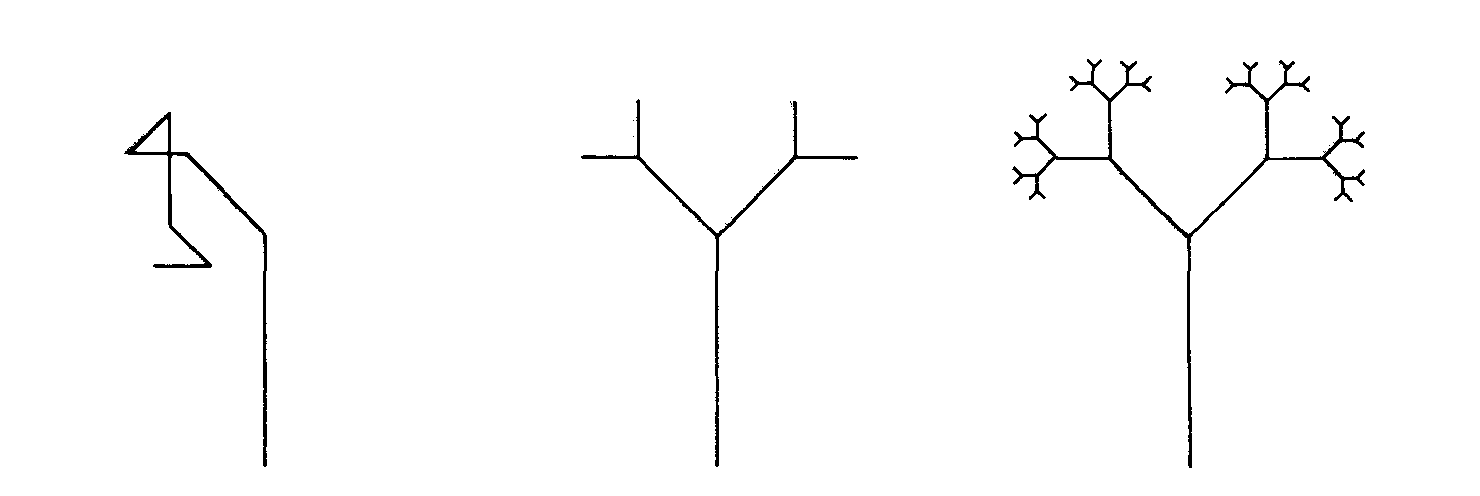
\includegraphics[scale=1]{fig2-19}
\caption{The \textsc{branch} procedure. (a) Version with state bug, \textsc{level} = 3. (b) Debugged version, \textsc{level} = 3. (c) Debugged version, \textsc{level} = 6.}
\end{center}
\end{figure}

Unfortunately, as shown in figure 2.19a, there is still a bug in the program. This bug, which is tricky to find, comes up often in such recursive descriptions: We must ensure that after drawing the left secondary
branch the turtle returns to the base of that branch, or else the \textsc{right} 90
instruction will not align the turtle correctly for drawing the right secondary branch. Ir1 other words, we must ensure that the process that draws
the left secondary branch restores the state of the turtle to what the
state was before the process began. The technical term for a process
that leaves the turtle in the same state in which it found it is state transparent.

\textsc{branch} will work only if its sub-branches are state-transparent. But
since the sub-branches as programs are just copies of \textsc{branch} itself,
\textsc{branch} must be made state-transparent. (In a recursive society all you
must do to make sure your offspring have some property is have it
yourself.) Here is the debugged program:

\begin{verbatim}
TO BRANCH (LENGTH, LEVEL)
   IF LEVEL = 0 THEN RETURN
   FORWARD LENGTH
   LEFT 45
   BRANCH (LENGTH/ 2, LEVEL - 1)
   RIGHT 90
   BRANCH (LENGTH/2, LEVEL - 1)
   ; turn and back up to make the
   ; procedure state-transparent
   LEFT 45
   BACK LENGTH
\end{verbatim}
Using this simple binary tree as a model, we can go on to construct
figures that look more like real trees. For example, we might add inputs
to the program to allow some other variation of the size of the secondary
branches besides ``divide by 2.'' Another possibility is to make the length
of stem depend not on the level, but on whether the stem belongs to a
left or a right sub-branch.

\begin{figure}
\begin{center}
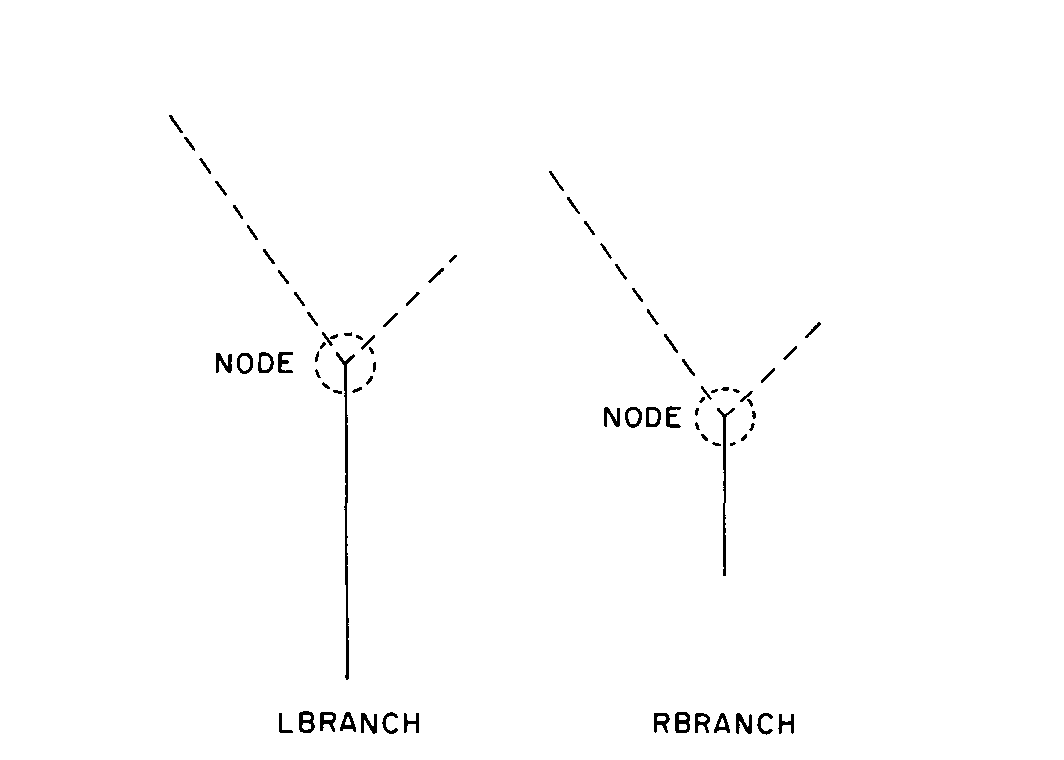
\includegraphics[scale=1]{fig2-20}
\caption{\textsc{lbranch} and \textsc{rbranch} have \textsc{node} in common}
\end{center}
\end{figure}

The cleanest way to implement this idea is to have separate left and
right procedures that produce stems of different lengths. As the dashed
lines in figure 2.20 indicate, each of these must prepare for the next-level
branch. Though the preparation is not hard, it is more than half the
procedure, and both left and right branch procedures must do it. So
it makes sense to make it a subprocedure called \textsc{node}. We can also
make \textsc{node} responsible for the stop rule, which is common to the two
procedures.

\begin{figure}
\begin{center}
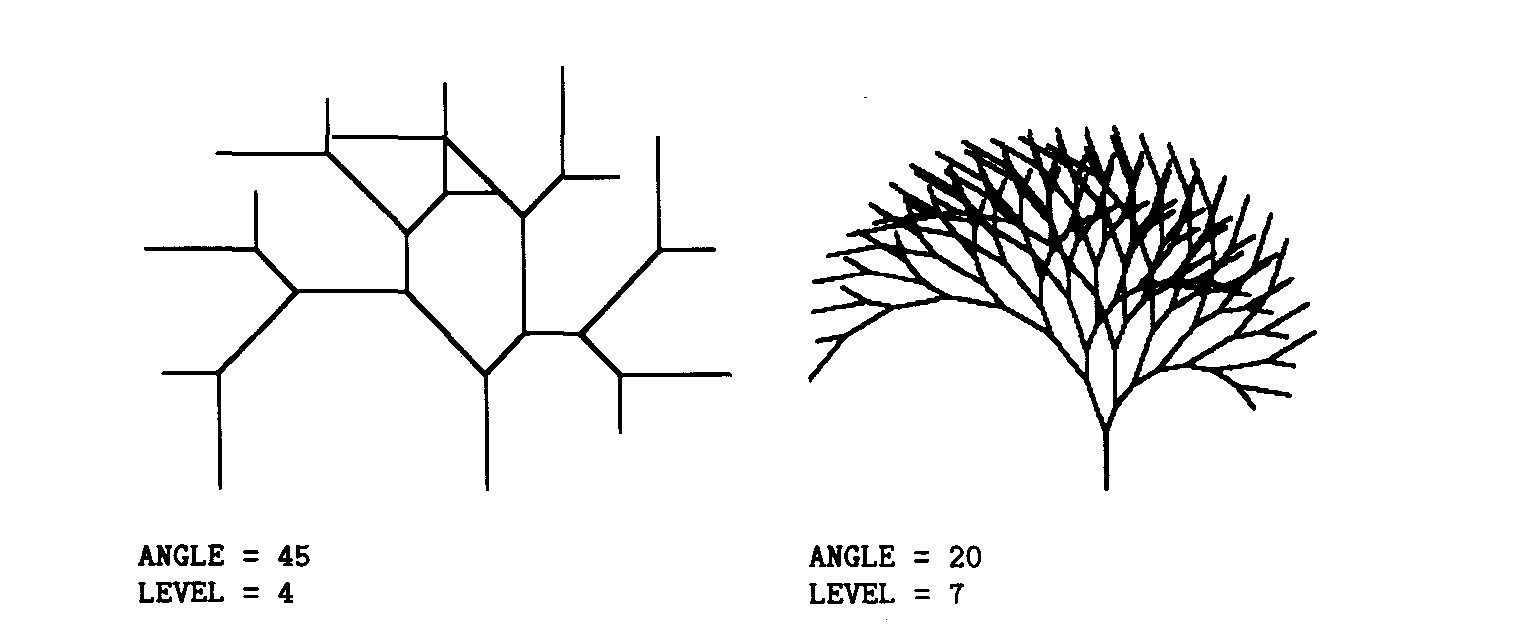
\includegraphics[scale=1]{fig2-21}
\caption{Branching figures drawn by \textsc{lbranch}}
\end{center}
\end{figure}


\begin{verbatim}
TO LBRANCH (LENGTH, ANGLE, LEVEL)
; draw a long stem
   FORWARD (2 * LENGTH)
   ; do next level
   NODE (LENGTH, ANGLE, LEVEL)
   ; make LBRANCH state-transparent
   BACK (2 * LENGTH)
   TO RBRANCH (LENGTH, ANGLE, LEVEL)
   ; draw a short stem
   FORWARD LENGTH
   ; do next level
   NODE (LENGTH, ANGLE, LEVEL)
   ; make RBRANCH state-transparent
   BACK LENGTH

TO NODE (LENGTH, ANGLE, LEVEL)
   IF LEVEL = 0 THEN RETURN
   ; point along left branch and draw it
   LEFT ANGLE
   LBRANCH (LENGTH, ANGLE, LEVEL - 1)
   ; draw right branch
   RIGHT (2 * ANGLE)
   RBRANCH (LENGTH, ANGLE, LEVEL - 1)
   ; make NODE state-transparent
   LEFT ANGLE
\end{verbatim}
You can start the process with either \textsc{lbranch} or \textsc{rbranch}. Figure 2.21
shows some of these trees. Notice that at first sight the growth pattern
looks random, even though it is actually very regular.
More information on the spiral shapes of shells, horns, claws, and teeth
can be found in On Growth and Form by D'Arcy Thompson (abridged
edition; Cambridge University Press, 1961). The branch procedure is
adapted from a model discussed in Patterns in Nature, by Peter S.
Stevens (Boston: Atlantic Monthly Press, 1974). Both of these books
are well worth having a look at if you are interested in mathematical
models in biology.

\subsubsection{Exercises for Section \thesection}

\begin{figure}
\begin{center}
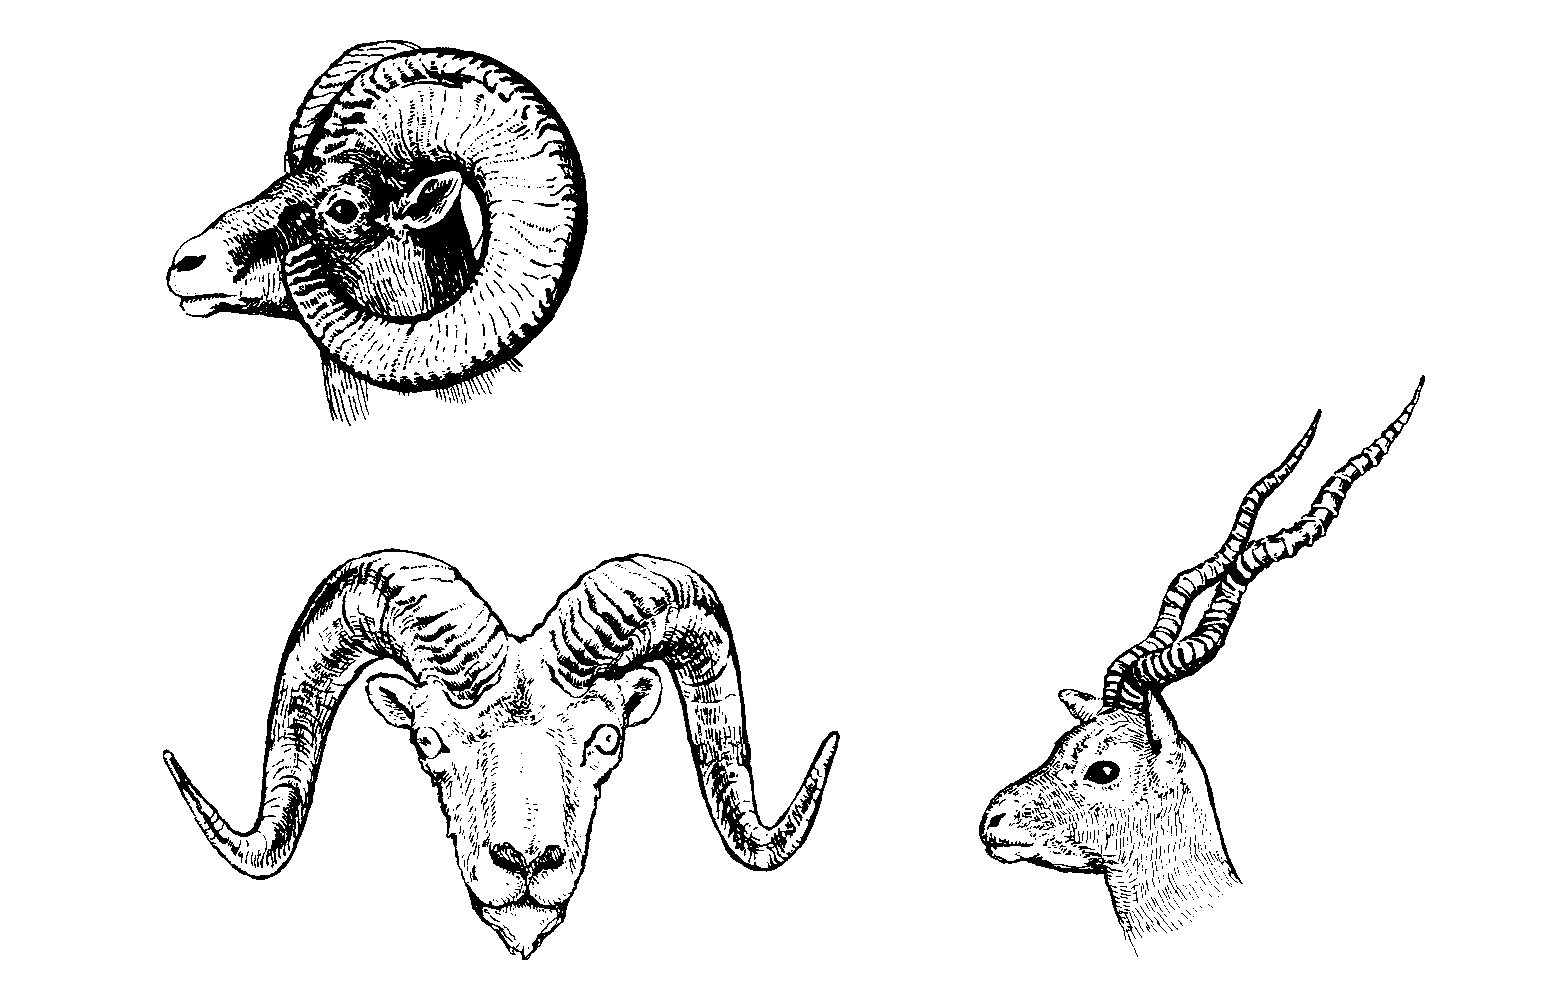
\includegraphics[scale=1]{fig2-22}
\caption{Examples of animal horns that can be modeled by \textsc{spiral.growth}}
\end{center}
\end{figure}

\begin{enumerate}
\item $[P]$ Figure 2.22 shows some animal horns. Can you find inputs to the
\textsc{spiral.growth} program that produce horns shaped like these?
\item $[P]$ Invent variants of the \textsc{spiral.growth} procedure in which the
chambers are not quadrilaterals.
\item $[P]$ Efficiency experts may object that our \textsc{spiral}\textsc{.growth} procedure
is inefficient in that the ratio of one chamber to the next should be
computed only once, rather than each time a new chamber is drawn.
But our version is easy to modify so that this ratio (and hence the shape
of the chambers) can be varied from one chamber to the next. We might
let the left and right sides grow more slowly (with a different ratio) than
the tops and bottoms, and so get a figure which becomes stubbier as it
grows. Experiment with possibilities like these. What kinds of shapes
arise if the change in growth is periodic (seasonal)? If the rate of growth
is random?
\item What is the total length of all the lines drawn by the \textsc{branch} procedure
for a given length and level?  
\item $[P]$ Modify \textsc{node} so that the choice of whether the left or the right
sub-branch is to be the long one is made randomly at each level.
\item Make a branching model in which each left sub-branch is twice as
long as each right sub-branch and sprouts two left-right branches. What
is the total length of all the branches drawn for a given length and level?
[HA]
\item $[P]$ Create some variations that introduce randomness into the model
given in the previous exercise. For instance, the left branch may sprout
either one or two branches at each level.
\item $[D]$ Does \textsc{eqspi (2, 2, 2), eqspi (1,1,1), eqspi (.5, .5, .5)},   approach
a limiting spiral the way \textsc{poly (n, n)} does, as $n$ goes to O? Explain why
or why not. How about \textsc{eqspi} $(n, n, n + 1)$? How about \textsc{eqspi} $(n, n, k^{n})$,
{\em k} constant? [A]
\item What parameters describe equiangular spirals the way radius or
curvature describes a circle? Relate these to the inputs of \textsc{eqspi}.  
\item $[D]$ Prove the assertion that any looping program which uses only
\textsc{s}\textsc{.forward}, \textsc{right}, and \textsc{grow} has an \textsc{eqspi} skeleton, paralleling the
results of section 1.3. What are the angle and the growth factor for
the steps of the skeleton?  

\end{enumerate}

\section{Recursive Designs}

The branching models of section 2.3 could be described as recursive
designs, because these figures contain subparts which are in some sense
equivalent to the entire figure (for example, a branch is made up of
branches). We've already run into two important considerations for
writing turtle procedures to generate such designs: We need to include
some kind of stop rule so that the process eventually stops generating
more and more subiigures, and we need to keep track of the state of the
turtle in designing the interface between part and subpart. ln particular,
it helps to make each part state-transparent.

\subsection{Nested Triangles}

\begin{figure}
\begin{center}
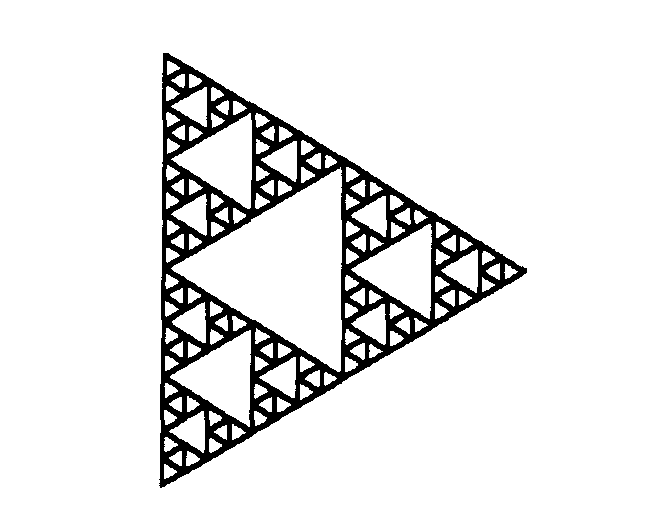
\includegraphics[scale=1]{fig2-23}
\caption{Figure drawn by \textsc{nested}\textsc{.triangle}}
\end{center}
\end{figure}

The nested triangle design shown in figure 2.23 illustrates these principles. The central observation is that the figure consists of a triangle
plus a smaller copy of itself at each corner, just as the trees of the
last section were forks plus smaller copies of themselves on each prong.
Thus, we imagine the turtle drawing our figure as follows: At each of
the vertices of the largest triangle, pause and construct a smaller figure
of half the size, in the corner. The smaller triangles should follow the
I same rules, drawing a still smaller triangle at each of their corners, and
so on, and so on. Finally, we'll stop generating subtriangles when the
sides get very small. All together, the procedure is

\begin{verbatim}
TO NESTED.TRIANGLE SIZE
   IF SIZE < 10 THEN RETURN
   REPEAT 3
      NESTED.TRIANGLE SIZE / 2
      FORWARD SIZE
      RIGHT 120
\end{verbatim}
Notice that each \textsc{nested}\textsc{.triangle(size)} will be state-transparent as
long as each \textsc{nested}\textsc{.triangle}\textsc{(size/2)} drawn in its corners satisfies
that property. In turn, that state transparency depends on the state
transparency of smaller and smaller \textsc{nested}\textsc{.triangle}s until, when \textsc{size}
is less than 10, the program stops, ensuring state transparency all the
way back up the line. A simple variation on this program draws smaller
figures outward from the corners:

\begin{verbatim}
TO CORNER.TRI SIZE
   IF SIZE < 10 THEN RETURN
   REPEAT 3
      FORWARD SIZE
      CORNER.TRI SIZE/2
      RIGHT 120
\end{verbatim}
Yet another way to interface a triangle to a recursive call to itself is to
stop halfway through a side and put the recursive call there:

\begin{verbatim}
TO OUTWARD.TRI SIZE
   IF SIZE < 10 THEN RETURN
   REPEAT 3
      FORWARD SIZE / 2
      INSERT SIZE
      FORWARD SIZE / 2
      RIGHT 120

TO INSERT SIZE
   LEFT 120
   OUTWARD.TRI SIZE/2
   ; ensure state transparency of INSERT
   RIGHT 120
\end{verbatim}
\begin{figure}
\begin{center}
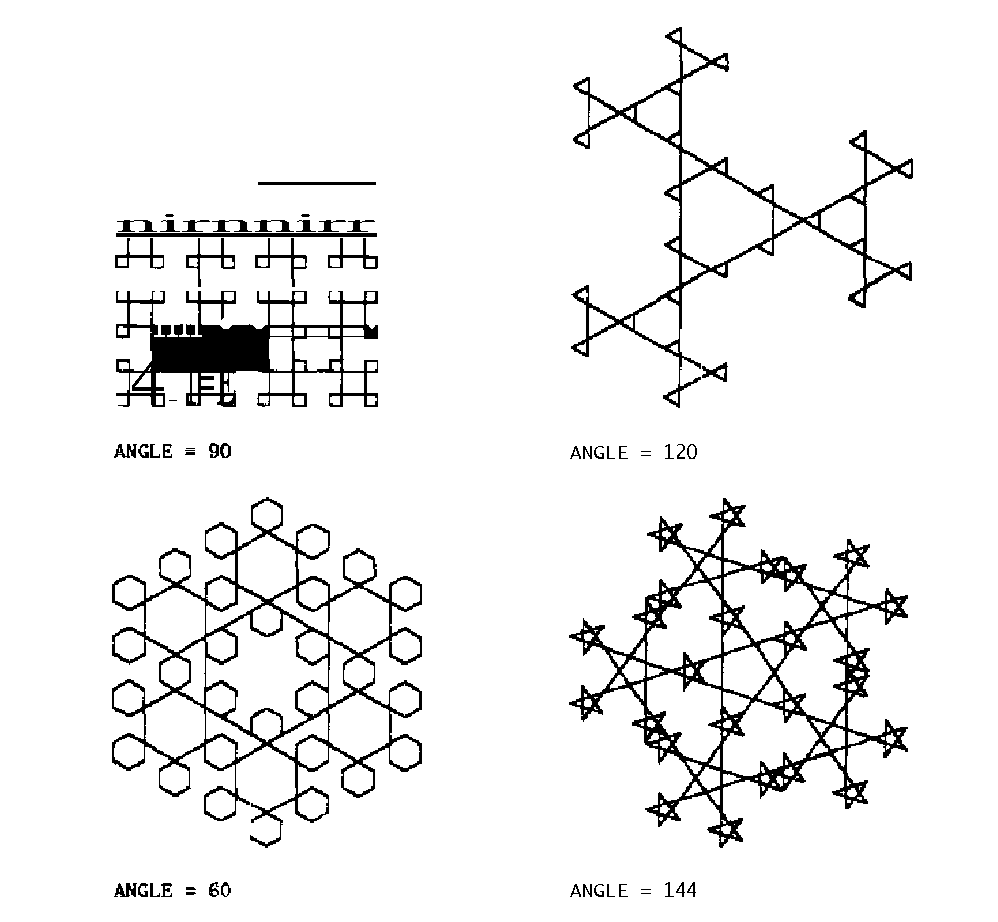
\includegraphics[scale=1]{fig2-24}
\caption{Shapes drawn by \textsc{cornerpoly}}
\end{center}
\end{figure}

\begin{verbatim}
TO NESTEDTRIANGLE (SIZE, LEVEL)
   IF LEVEL = 0 THEN RETURN
   REPEAT 3
      NESTEDTRIANGLE (SIZE/2, LEVEL - 1)
      FORWARD SIZE
      RIGHT 120
\end{verbatim}
These triangle procedures can be generalized to arbitrary \textsc{poly} figures.
The only tricky part is to make sure we know how many sides to draw,
say, as a function of the \textsc{poly}'s angle. As we saw in chapter 1, this
can be done by accumulating total turning and stopping when the total
turning is a multiple of $360^{\circ}$:

\begin{verbatim}
TO CORNERPOLY (SIZE, ANGLE, TOTALTURN)
   IF SIZE < 10 THEN RETURN
   REPEAT
      CORNERPOLYSTEP (SIZE, ANGLE)
      TOTALTURN <- TOTALTURN + ANGLE
      UNTIL REMAINDER (TOTALTURN, 360) = 0

TO CORNERPOLYSTEP (SIZE, ANGLE)
   FORWARD SIZE
   CORNERPOLY (SIZE/2, - ANGLE, O)
   ; using - ANGLE “symmetrizes” the figure
   RIGHT ANGLE
\end{verbatim}
The \textsc{cornerpoly} procedure is invoked with the third input, \textsc{totalturn},
equal to zero. Figure 2.24 shows some samples drawn by this program.
Although we've been using the side length as a stop rule for these
designs, you might prefer to stop at a particular level of recursion. For
example,

\subsection{Snowflakes and Other Curves}

In some instances the effect of state transparency can be achieved although there is not true state transparency. In such cases, each procedure knows the state change of its subprocedures and hence knows
what to do to compensate (if necessary). If the state change of the subprocedure is simple there are few disadvantages to this method, and if
the state change is exactly what the main procedure needs to prepare
for a next step this method can be advantageous.
This strategy is illustrated by a program to draw the snowflake curve
shown in figure 2.25. Think of this curve as a triangle in which each side
is made up of four subsides, each subside is made up of four sub-subsides,
$p$ etc. Rather than making the procedure state-transparent, we'll design
each side to move the turtle forward a certain distance without changing
the heading:

\begin{verbatim}
TO SNOWFLAKE (SIZE, LEVEL)
   REPEAT 3
   SIDE (SIZE, LEVEL)
   RIGHT 120
   TO SIDE (SIZE, LEVEL)
   IF LEVEL = 0 THEN
      FORWARD SIZE
      RETURN
   SIDE (SIZE/3, LEVEL - 1)
   LEFT 60
   SIDE (SIZE/3, LEVEL - 1)
   RIGHT 120
   SIDE (SIZE/3, LEVEL - 1)
   LEFT G0
   SIDE (SIZE/3, LEVEL - 1)
\end{verbatim}
Until now the \textsc{level} = 0 process has been trivial, and has been statetransparent by virtue of doing nothing at all. Here the \textsc{level} = 0 action
is crucial so that the \textsc{level} = 1 process gets the state change expected,
\textsc{forward(size)}. In fact, in the snowilake procedure no \textsc{forward} commands will be issued except when \textsc{level} = 0.

\begin{figure}
\begin{center}
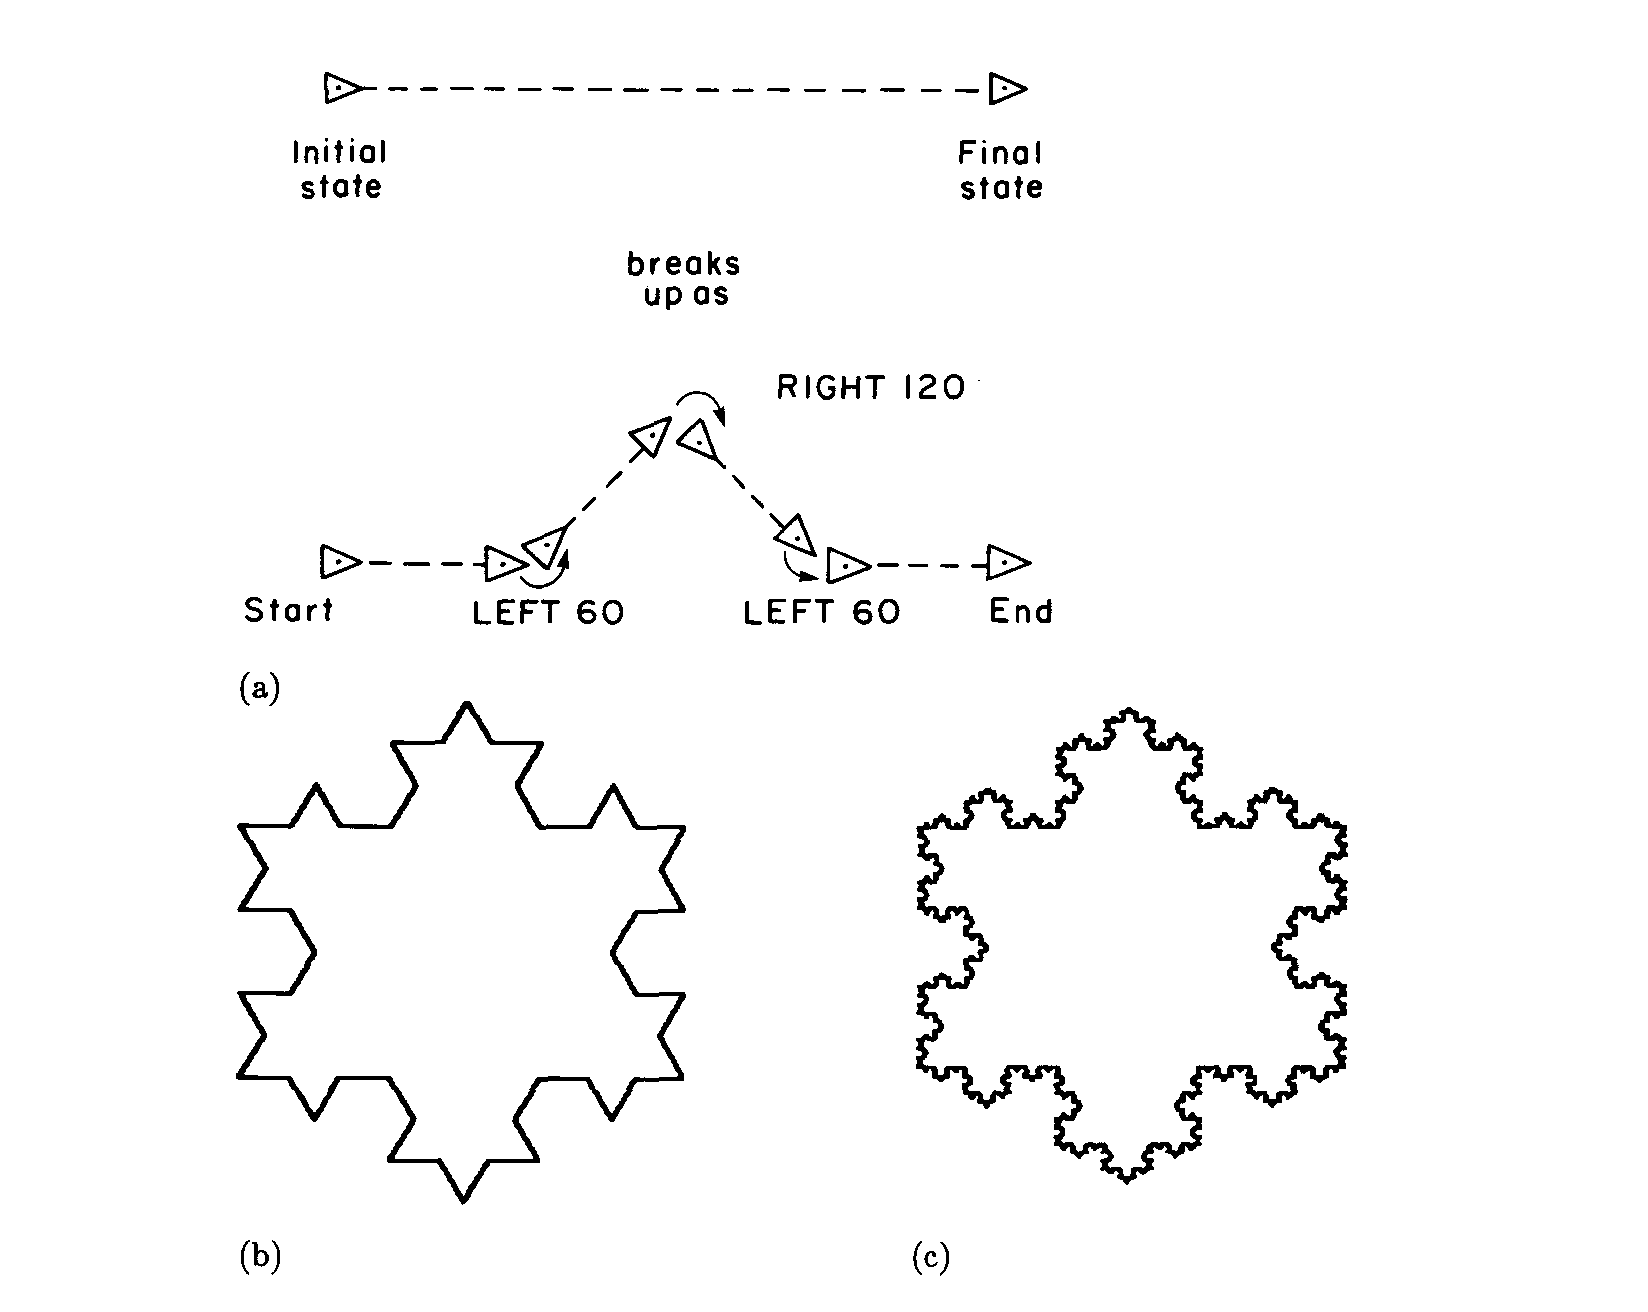
\includegraphics[scale=1]{fig2-25}
\caption{The snowflake curve. (a) Recursive decomposition of a ``side.'' (b) Snowflake, \textsc{level} = 2. (c) Snowflake, \textsc{level} = 4}
\end{center}
\end{figure}


Another related curve is the ``C curve'' shown in figure 2.26a. A level
0 C curve is just a line; a level $n$ C curve consists of two level $n - 1$ C
curves at right angles to each other, followed by a $90^{\circ}$ turn to restore
the heading:

\begin{verbatim}
TO C (SIZE, LEVEL)
   IF LEVEL = 0 THEN
      FORWARD SIZE
      RETURN
   C (SIZE, LEVEL - 1)
   RIGHT 90
   C (SIZE, LEVEL - 1)
   LEFT 90
\end{verbatim}
\begin{figure}
\begin{center}
\includegraphics[scale=1]{fig2-26}
\caption{(a) C curve, \textsc{level} = 10. (b) Dragon curve, \textsc{level} = 11}
\end{center}
\end{figure}

The ``dragon curve'' shown in figure 2.26b is similar to the C curve;
however, there is only one $90^{\circ}$ turn, and its direction changes from level
to level. We can think of it as generated by a pair of procedures \textsc{ldragon}
and \textsc{rdragon} specified as follows: A level $n$ \textsc{ldragon} is made up of a level
$n - 1$ \textsc{ldragon} and a level $n - 1$ \textsc{rdragon} with a left turn in between; a
level $n$ \textsc{rdragon} is made up of a level $n - 1$ \textsc{ldragon} and a level $n - 1$
\textsc{rdragon} with a right turn in between; a level 0 dragon is a line:

\begin{verbatim}
TO LDRAGON (SIZE, LEVEL)
   IF LEVEL = 0 THEN
      FORWARD SIZE
      RETURN
   LDRAGON (SIZE, LEVEL - 1)
   LEFT 90
   RDRAG0N (SIZE, LEVEL - 1)
   TO RDRAGON (SIZE, LEVEL)
   IF LEVEL = 0 THEN
      FORWARD SIZE
      RETURN
   LDRAGON (SIZE, LEVEL - 1)
   RIGHT 90
   RDRAGON (SIZE, LEVEL - 1) 
\end{verbatim}
\subsection{Space-Filling Design}

Suppose we write a program that draws something inside a square. For
the moment, we won't care what the program does, but we will insist
that the initial and final states of the turtle are related to the square
as shown in figure 2.27a. Consider a new square that consists of nine
smaller squares. We can use our simple program in each smaller square
to produce a more complicated program winding through the new square
(figure 2.27b). All we need is appropriate interfacing between subsquares.
This more complicated program relates to the new square in exactly
the same way that the simple program related to the first square, so we
can continue this process. In the end we will have a square, consisting of
nine smaller squares, each of which consists of still smaller squares, and
I so on. The process is recursive, and can be implemented in the usual
way (by writing the higher-level procedure in terms of the lower-level
one). The interfaces between the various subfigures are shown in figure
2.27b. For a level 0 process, we can use the simplest possible way of
entering and leaving a square, as assumed --- \textsc{forward(size)}. This gives
the following procedure:

\begin{verbatim}
TO FILL (SIZE, LEVEL)
   IF LEVEL = 0 THEN
      FORWARD SIZE
      RETURN
      ; side of small square is 1/3 side of large square
   FILL (SIZE / 3, LEVEL - 1)
   ; interface to next subfigure is LEFT 90
   LEFT 90
   FILL (SIZE / 3, LEVEL - 1)
   ; next three subfigures have RIGHT 90 as interface
   REPEAT 3
      RIGHT 90
      FILL (SIZE / 3, LEVEL - 1)
      ; next three have LEFT 90 as interface
   REPEAT 3
      LEFT 90
      FILL (SIZE / 3, LEVEL - 1)
      ; final subfigure has RIGHT 90 interface
   RIGHT 90
   FILL (SIZE / 3, LEVEL - 1)
\end{verbatim}
\begin{figure}
\begin{center}
\includegraphics[scale=1]{fig2-27}
\caption{The \textsc{fill} procedure. (a) Initial and final states for traversing a square. (b) Traversing the square, decomposed into traversing nine subsquares plus left-right interfacing. (c-e) The pattern drawn by \textsc{fill} at \textsc{level} = 1, 2, and 4.}
\end{center}
\end{figure}

This \textsc{fill} procedure is an example of a space-filling design. lf we
make \textsc{level} greater and greater, then the \textsc{fill} curve winds through the
square in finer and finer subdivisions. For \textsc{level} very large, we could
imagine \textsc{fill} as passing through every point of the square. \textsc{fill}, as
written, draws a curve that intersects itself; however, it is possible to
separate the nine subsquares with small interfaces to avoid intersection.
(See exercise 5.) If done properly, this will not affect the space-filling
property of the design.

\begin{figure}
\begin{center}
\includegraphics[scale=1]{fig2-28}
\caption{The Hilbert curve. (a) \textsc{level}=2 (b) \textsc{level}=3 (c) \textsc{level}=5 (d) Turtle ``traverses'' square by traversing each subsquare. (e) Decomposition of level $n$ Hilbert curve into four level $n - 1$ curves together with interfaces. (f) Details of interfacing}
\end{center}
\end{figure}

Perhaps the most famous space-filling design is the curve (shown in
figure 2.28) invented by the German mathematician David Hilbert. As
indicated in figure 2.28e, we can think of the level $n$ Hilbert curve as
made up of four level $n - 1$ Hilbert curves, joined by interfaces which
are straight line segments. Another way to picture this is to imagine the
square as divided into four subsquares. The Hilbert curve traverses the
square by visiting each of the subsquares and placing the interfaces in
between. (See figure 2.28d.)

In designing a program to draw the Hilbert curve we must be careful
to keep track of how each level of the curve affects the state of the turtle.
Assume that the turtle begins facing along the edge of the square that
it traverses, and ends in the same direction. Then pasting together four
level $n - 1$ curves to form the level n curve requires interface turns as
shown in figure 2.28f. A second tricky point is that there are really two
different level $n - 1$ Hilbert curves-one that traverses its square to the
left and one that traverses to the right-and that the level $n$ curve is
made up of two of each parity. Finally, notice that the interfaces alone
provide the state change assumed at each level, so we can let the level
0 curve be simply a point; then the interfaces in level 1 will provide the
state change assumed by higher levels. The complete program consists
of two procedures, \textsc{lhilbert} and \textsc{rhilbert}:

\begin{verbatim}
TO LHILBERT (SIZE, LEVEL)
   IF LEVEL = 0 THEN RETURN
   ; rotate and draw first subcurve
   ; with opposite parity to big curve
   LEFT 90
   RHILBERT (SIZE, LEVEL - 1)
   ; interface to and draw second subcurve
   ; with same parity as big curve
   FORWARD SIZE
   RIGHT 90
   LHILBERT (SIZE, LEVEL - 1)
   ; third subcurve
   FORWARD SIZE
   LHILBERT (SIZE, LEVEL - 1)
   ; fourth subcurve
   RIGHT 90 \textsc{forward} SIZE
   RHILBERT (SIZE, LEVEL - 1)
   ; a final turn is needed to make the turtle
   ; end up facing outward from the large square
   LEFT 90
\end{verbatim}
The \textsc{rhilbert} procedure is the same, but with all the turns reversed:

\begin{verbatim}
TO RHILBERT (SIZE, LEVEL)
   IF LEVEL = 0 THEN RETURN
   RIGHT 90
   LHILBERT (SIZE, LEVEL - 1)
   FORWARD SIZE
   LEFT 90
   RHILBERT (SIZE, LEVEL - 1)
   FORWARD SIZE
   RHILBERT (SIZE, LEVEL - 1)
   LEFT 90
   FORWARD SIZE
   LHILBERT (SIZE, LEVEL - 1)
   RIGHT 90
\end{verbatim}
We ean combine \textsc{lhilbert} and \textsc{rhilbert} into a single procedure by
providing a third input, equal to $+1$ or $-1$, whose sign is reversed to
convert left turns to right turns:

\begin{verbatim}
TO HILBERT (SIZE, LEVEL, PARITY)
   IF LEVEL = 0 THEN RETURN
   LEFT (PARITY * 90)
   HILBERT (SIZE, LEVEL - 1, - PARITY)
   FORWARD SIZE
   RIGHT (PARITY * 90)
   HILBERT (SIZE, LEVEL - 1 , PARITY)
   FORWARD SIZE
   HILBERT (SIZE, LEVEL - 1, PARITY)
   RIGHT (PARITY * 90)
   FORWARD SIZE
   HILBERT (SIZE, LEVEL - 1, - PARITY)
   LEFT (PARITY * 90)
\end{verbatim}
\subsubsection{Exercises for Section \thesection}

\begin{enumerate}
\item $[P]$ Try the following variant of the nested-triangle procedure, which
adds only one smaller triangle at each level connecting the midpoints of
the larger triangle:

\begin{verbatim}
TO NEST (SIZE, LEVEL)
   IF LEVEL = 0 THEN STOP
   FORWARD SIZE / 2
   SUBNEST (SIZE, LEVEL)
   FORWARD SIZE / 2
   RIGHT 120
   FORWARD SIZE
   RIGHT 120
   FORWARD SIZE
   RIGHT 120

TO SUBNEST (SIZE, LEVEL)
   RIGHT 60
   NEST (SIZE / 2, LEVEL - 1)
   LEFT GO
\end{verbatim}
Generalize this procedure to produce designs based on nested \textsc{poly}s.
[HA]
\item What is the length of the level n snowflake curve? How much area
does it enclose? [HA]
\item $[P]$ Write a procedure that generalizes the (triangular) snowflake curve
to produce arbitrary ``polysnowflakes.''
\item $[D]$ What is the length of the level $n$ Hilbert curve?  
\item $[P]$ The \textsc{fill} curve is not as elegant as it might be because it intersects
itself. Add interfaces, in the same way that \textsc{hilbert} has them, to
separate the squares a bit. (See figure 2.29.) Note that the net effect of
the interfaces by themselves (including turning to set up for diagonals)
is the state change assumed for each level of \textsc{fill}. This is the same as
with the interfaces to \textsc{hilbert}, and makes it possible to allow the level
0 curve to be simply \textsc{return}. Try this possibility for \textsc{fill} as well.
\item $[P]$ The Hilbert curve is constructed on the following model: (1) Walk
along the side of a square, and imagine filling the square. (2) Divide
the square into four subsquares. Construct a similar space-filling curve
A based on dividing a triangle into four subtriangles.

\begin{figure}
\begin{center}
\includegraphics[scale=1]{fig2-29}
\caption{Interfaces to \textsc{fill} and resulting (level 2) design}
\end{center}
\end{figure}

\item $[P]$ Construct a space-filling curve on the Hilbert model, but based
on dividing a square into nine subsquares.
\item $[PD]$ Write a procedure to draw the space-filling curve shown in figure
2.30. (This curve was invented by the Polish mathematician Wraclaw
Sierpinski.)  
\item $[P]$ Invent some new space-filling designs.
\item $[P]$ Can you build a recursive design like \textsc{fill} or \textsc{hilbert}, but based
on entering the middle of the side of the square rather than the corner?
\item $[P]$ How much does the \textsc{fill} curve depend on the particular level
0 step used? Does \textsc{fill} change its character if you use some more
complicated level 0 step than \textsc{forward(size)}?
\item $[P]$ Notice that in none of our recursive designs does the turtle
have any representation of the curve except the program itself. On
the other hand, by encoding turtle commands as letters, one can construct an explicit representation in the following way: Let F stand for
\textsc{forward} SIZE, L for \textsc{left} 60, and R for \textsc{right} 120; then construct a
string representing the side of a snowflake curve with the rules
$$S_0 = F$$
$$S_n = S_{n-1}LS_{n-1}RS_{n-1}LS_{n-1}$$

In fact a program to draw the side could be enacted as follows: Initialize
$S \leftarrow F$ ; apply the recursive step $S \leftarrow SLSRSLS$ (juxtaposition denotes
concatenation) $n$ times; have the turtle interpret the resulting string.
Try this with several known recursive designs, such as \textsc{hilbert} and
\textsc{snowflake}. Now explore the possibilities of this ``word generation''
method by varying level 0, the recursive step, and the interpretation of
letters. You may wish to add more variable symbols to the process,
for example, $T \leftarrow SRSLSRS$.

\begin{figure}
\begin{center}
\includegraphics[scale=1]{fig2-30}
\caption{The Sierpinski curve}
\end{center}
\end{figure}

\item $[PD]$ All our recursive designs have maintained the constraint that
turtle must not lift the pen. Thus, the recursive step in \textsc{fill} consisted
of taking a certain walk through a square and then using that walk nine
times in sequence to make a more complex walk through a square. But
I we could just as easily imagine taking any design whatsoever in a square
(not necessarily a walk through it) and gluing nine copies to make a
larger square (without making sure the designs hook up simply). (See
I figure 2.31a.) Of course the overall design will appear more impressive
if some lines do ``accidentally'' hook up. This is like tiling a floor
with more and more complex tiles. Varying the design on the level
0 tile together with the orientations for the tiles in the recursive step
makes a fascinating artistic and mathematical exploration. To aid the
exploration you may wish to implement the recursive gluing-together
steps as programs that can take arbitrary design-drawing programs,
including glued-together designs, as inputs. That way a level 3 recursive
tile will look like \textsc{glue1(glue2(glue3(shape1)))}. Figure 2.31b-e shows
designs that can be made in this way. See if you can find the level 0
design in each.
\end{enumerate}

\chapter{Vector Methods in Turtle Geometry}
\begin{quote}
I am sorry that I had to torture you with these
elements of analytic geometry. The purpose of this
invention of Descartes' is nothing but to give names
to the points $X$ in a plane by which we can distinguish and recognize them. This has to be done in a
systematic way because there are infinitely many of
them; and it is the more necessary as points, unlike
persons, are all completely alike, and hence we can
distinquish them only by attaching labels to them.

Hermann Weyl, {\em Symmetry}
\end{quote}

In chapter 1 we emphasized how turtle geometry provides an alternative to Cartesian coordinates for exploring geometry with a computer display screen. This chapter introduces a third way to represent
geometric phenomena: vector representation. Vectors methods are, in
many ways, intermediate between pure turtle methods and coordinate
methods. We will be making use of vectors as a mode of representing
geometric phenomena that is sufficiently intrinsic and local to capture
simply some essential features of turtle geometry but also shares the algebraic nature that makes analytic geometry so generally useful. More
than that, the algebra of vectors is easily reduced to simple arithmetic
operations through the introduction of vector coordinates. Since they
link well with geometry on one side and with numerical calculation on the
other, vectors are an ideal representation to use in computer programs
dealing with geometry. Using this fact, we will show how to implement
turtle geometry from scratch on almost any computer graphics system,
how to extend turtle geometry into three dimensions, and (in later chapters) how to design exotic turtles that walk on cubes, on spheres, and
even in Einstein's curved spacetime.

Despite this great power and the detailed work necessary to harness
it, we encourage you not to lose sight of the most important reason
for a combined look at turtles and vectors: Turtle geometry and vector
geometry are two different representations for geometric phenomena,
and whenever we have two different representations of the same thing
we can learn a great deal by comparing representations and translating
descriptions from one representation into the other. Shifting descriptions
back and forth between representations can often lead to insights that
are not inherent in either of the representations alone.

We will start this chapter by looking at some of the familiar turtle
phenomena --- \textsc{poly}s, closed paths, and so on --- in terms of vectors. After
dealing with vectors as conceptual entities, we will reduce vectors to
coordinates and thus gain the ability to manipulate vectors on the computer.

\section{Vector Analysis of Turtle Programs}

The turtle commands \textsc{forward}, \textsc{back}, \textsc{left}, and \textsc{right} describe changes
relative to the turtle's current state. For example, the pair of commands
\textsc{right} 90, \textsc{forward} 100 results in a motion of 100 steps from the turtle's
current position and at $90^{\circ}$ from the current heading. This relativity is
exactly what allows turtle programs to be simple intrinsic descriptions
of shapes such as circles and \textsc{poly}s. However, if you have a global frame
of reference in mind, and absolute orientation is important to you, the
two shapes in figure 3.1a are very different; one is a square and one is
A a diamond. The orientation of the sides with respect to a global ``up''
allows one to discriminate between square and diamond, even though
intrinsically the two figures are identical. In this case, position is still
relative. One cannot transform ``squareness'' to ``diamondness'' simply
by changing the position of the figure without rotating it.

Motions that are absolute in direction but relative in position --- called
displacements --- are readily described by {\em vectors}. We can think of a
vector as an arrow of definite length and direction but arbitrary position,
pointing from beginning to end of the displacement. (Throughout the
book we denote vectors by boldface symbols such as \textbf{v} and \textbf{w}.) ln order
to make a turtle produce squares and diamonds, imagine handing it
a collection of vectors. A program to draw a figure tells the turtle
when to make the displacement described by each vector. The following
procedures correspond to figure 3.1b and c.

\begin{verbatim}
TO SQUARE
   DISPLACE.BY S1
   DISPLACE.BY S2
   DISPLACE.BY S3
   DISPLACE.BY S4

TO DIAMOND
   DISPLACE.BY D1
   DISPLACE.BY D2
   DISPLACE.BY D3
   DISPLACE.BY D4
\end{verbatim}
\begin{figure}
\begin{center}
\includegraphics[scale=1]{fig3-1}
\caption{(a) Rotating a square produces a diamond. (b-c) Vector decompositions of square and diamond}
\end{center}
\end{figure}

\subsection{Vector Operations: Scalar Multiplication and Addition}

There are a number of relations between vectors that can be useful
to a vector-following turtle. If the turtle knows how to walk along a
particular vector $-$\textbf{v}, then it should be able to walk along a vector of
the same length pointing in exactly the opposite direction. Naturally
enough, we denote this displacement by $-$\textbf{v}. Similarly, a displacement
in the direction of \textbf{v}, but 5 times as far, can be denoted by $5 \times \textbf{v}$ (or simply
$5\textbf{v}$). In general, $a\textbf{v}$ (where $a$ is a number) is a vector in the direction of \textbf{v},
but {\em a} times as long. (If {\em a} is negative, $a\textbf{v}$ is opposite in direction.) This
operation is called scalar multiplication of numbers and vectors. It is
essentially just changing the scale used to measure displacement. Scalar
division can be defined by the formula $\textbf{v}/a = (1 / a) \times \mathbf{v}$.

Besides scalar multiplication (and the special case $-1 \times \textbf{v} = -\textbf{v}$)
there is one other fundamental method of producing new vectors from
old ones. Observe that performing two displacements in sequence defines
a net displacement, a net change in position. A displacement \textbf{v} followed
by a displacement \textbf{w} yields a net displacement called the vector sum,
denoted \textbf{v}+\textbf{w}. Having defined addition of vectors, we can define vector
subtraction as adding the negative:
$$\textbf{v} - \textbf{w} = \textbf{v} + (-\textbf{w}) (\text{by definition}).$$

Vector addition satisfies the commutative property
$$\textbf{v} + \textbf{w} = \textbf{w} + \textbf{v}$$
\noindent for any vectors \textbf{v} and \textbf{w}. This is illustrated in figure 3.2a, which shows
how following along \textbf{v} and then along \textbf{w}, or alternatively \textbf{w} and then \textbf{v},
forms a parallelogram whose diagonal is the vector sum.

Figures 3.2b and c illustrate two more simple but important formulas
that relate scalar multiplication to addition of vectors:
$$(a+b)\textbf{v}=a\textbf{v}+b\textbf{v}$$
$$a(\textbf{v} + \textbf{w}) = a\textbf{v} + a\textbf{w}$$
\noindent The special vector \textbf{0} represents no displacement at all; its length is
zero. This zero vector is analogous to the number zero, and it has many
of the same properties:
$$\textbf{v} - \textbf{v} = \textbf{0}$$
$$\textbf{0} + \textbf{v} = \textbf{v}$$
$$\textbf{0} \times \textbf{v} = \textbf{0}$$
\begin{figure}
\begin{center}
\includegraphics[scale=1]{fig3-2}
\caption{Properties of vector addition}
\end{center}
\end{figure}

\subsection{Vector Representations of Closed Paths}

Now we'll take advantage of vectors to rephrase some of our analyses of
familiar turtle-geometric programs and look at some new phenomena.
We will be using the following fundamental correspondence between vectors and turtle programs: Each \textsc{forward} step by the turtle is a displacement and can be described by a vector; successive displacements can
be described by vector addition. Notice that the \textsc{right} and \textsc{left} commands are not directly represented by vectors; rather, they determine
the direction of the vectors generated by \textsc{forward} commands.
Suppose the turtle makes its first move according to some initial vector \textbf{$\mathbf{v_0}$}. If the second move is along \textbf{$\mathbf{v_1}$}, then the net displacement is just
\textbf{$\mathbf{v_o}$} + \textbf{$\mathbf{v_l}$}. The turtle's net displacement after n steps, as shown in figure
3.3, will be
$$\mathbf{v_0} + \mathbf{v_1} + \cdot \cdot \cdot + \mathbf{v_{n-1}}$$

\begin{figure}
\begin{center}
\includegraphics[scale=1]{fig3-3}
\caption{Turtle's displacement as a sum of vectors}
\end{center}
\end{figure}

If the path is closed in these n steps the turtle must have returned to
its starting point, and thus the net displacement from the initial position
must be zero:
$$\mathbf{v_0}+\mathbf{v_1}+ \cdot \cdot \cdot + \mathbf{v_{n-1}} = \mathbf{0}$$

So if we ignore the question of whether or not the turtle's final heading
is the same as its initial heading, then we can say the turtle's path is
closed precisely when the vectors that represent the position changes
add up to zero.

\subsection{POLY Revisited: Rotations and Linearity}

Let's look carefully at a simple special case: \textsc{poly}, our archetypal looping
program from chapter 1. We'll give a new interpretation of the \textsc{poly}
closing theorem of subsection 1.2.2. To keep things simple let the \textsc{angle}
of the \textsc{poly} be 360/$n$, where $n$ is a positive integer. The \textsc{poly} closing
theorem says closure will be achieved in n steps. Reinterpreting the
closure in terms of vectors, we see that proving the theorem boils down
to verifying the equation
$$\mathbf{v_0}+\mathbf{v_1}+ \cdot \cdot \cdot +\mathbf{v_{n-1}} = \mathbf{0}$$
\noindent In order to do this we need some way of capturing in vector terms the
simple relationship among the vs: They are all just \textbf{$v_0$} rotated by various
multiples of the \textsc{poly} angle. To express this relation we define, for any
vector \textbf{v} and angle $A$, a new vector Rotate(\textbf{v},$A$), also written $R_A$(\textbf{v}),
to be the vector obtained by rotating \textbf{v} through $A$. Using this rotation
operation allows us to express the special property of the \textsc{poly} segments:
\textbf{$v_k$} = $R_{kA}$(\textbf{$v_0$}) $(A = 360/n)$

\begin{figure}
\begin{center}
\includegraphics[scale=1]{fig3-4}
\caption{Linearity of the rotation operation}
\end{center}
\end{figure}

Now we can restate the \textsc{poly} closing theorem as follows:

\noindent
\textbf{\textsc{POLY} Closing Theorem (Vector Form)} Given any vector $\mathbf{v_0}$ and positive
integer $n$, let $A = 360/ n$ and let $\mathbf{v_k} = R_{kA}(\mathbf{v_0})$. Then
$$\mathbf{v_0}+\mathbf{v_1}+\cdot \cdot \cdot+\mathbf{v_{n-1}} = \mathbf{0}$$

The proof of this theorem will be based on two fundamental properties
of the rotation operation $R_A$ for any angle $A$. As figure 3.4a illustrates,
the rotation of any scalar multiple of a vector v can be obtained simply
by scaling $R_A(\mathbf{v})$:
$$R_A(a\mathbf{v}) = aR_A(\mathbf{v})$$
\noindent This is called the scaling property of rotation. Rotation has another
property called additivity, which means that for any vectors \textbf{v} and \textbf{w}
$$R_A(\mathbf{v} + \mathbf{w}) = R_A(\mathbf{v}) + R_A(\mathbf{w})$$
\noindent Figure 3.4b demonstrates that rotation satisfies additivity; just rotate
the whole picture for vector addition and note that each of the parts \textbf{v}
and \textbf{w} and the sum \textbf{v} + \textbf{w} get rotated while preserving their configuration
as a sum. lf an operation has both the scaling and additivity properties,
then it is said to be linear. Linearity will soon take its place beside local
vs. global and intrinsic vs. extrinsic as one of the recurring mathematical
themes of this book. 

Returning to the \textsc{poly} theorem, we wish to demonstrate that the sum
$$\mathbf{V} = \mathbf{v_0} + \cdot \cdot \cdot + \mathbf{v_{n-1}}$$
\noindent satisfies \textbf{V} = \textbf{0}. The insight that proves this is that the collection of \textbf{v}s
that make up \textbf{V} is perfectly symmetrical. The sum of them could hardly
point in any direction favoring one \textbf{v} over another, and so must point in
no direction at all: \textbf{V} = \textbf{0}.

To turn this observation into a proof, let us rotate \textbf{V} through angle $A$
and use linearity:
$$R_A(\mathbf{V}) = R_A(\mathbf{v_0} + \mathbf{v_1} + \cdot \cdot \cdot + \mathbf{V_{n-1}}) = R_A(\mathbf{v_0}) + R_A(\mathbf{v_1}) + \cdot \cdot \cdot + R_A(\mathbf{v_{n-1}})$$
\noindent But $R_A(\mathbf{v_0}) = \mathbf{v_1}$ (by the definition of $\mathbf{v_k}$), and in general each $\mathbf{v_k}$ is
transformed into $\mathbf{v_{k+1}}$ all the way until $\mathbf{v_{n_1}}$, which gets transformed
into $\mathbf{v_0}$ (since $nA = 360$). Therefore,
$$R_A(\mathbf{V}) = \mathbf{v_1} + \mathbf{v_2} + \cdot \cdot \cdot +\mathbf{v_{n-1}} + \mathbf{v_0} = \mathbf{V} $$
Note that the last equality follows from commutativity of vector addition
(the fact that order doesn't matter in a sum).
Having demonstrated that \textbf{V} doesn't change when rotated by $A$, we
complete the proof by observing that the only vector that can remain
unchanged by a rotation is the zero vector. (This statement is geometrically obvious, although later on we'll develop the machinery to prove
this using algebra rather than geometry; see exercise 2 of section 3.2.)

In summary,
$$R_A(\mathbf{V}) = \mathbf{V} \text{ implies that } \mathbf{V} = \mathbf{0}$$
\noindent and this completes the proof of the theorem.

\begin{figure}
\begin{center}
\includegraphics[scale=1]{fig3-5}
\caption{The \textsc{poly} equation $v_0 + v_1 + . . . v_k = c + R_{kA}(\mathbf{r_0})$}
\end{center}
\end{figure}

We began this chapter by introducing vectors as a more global method
of describing turtle paths. We can capitalize on that perspective by
phrasing a global description of \textsc{poly} in terms of vectors. The description
we have in mind specifies that the vertices of \textsc{poly} lie on a fixed circle
where the angular measure of the arc between vertices is exactly the
angle input to the \textsc{poly} (see chapter 1, section 1.2, exercise 15). This
fact means that, instead of following along \textsc{poly} segments to reach a
particular vertex, we can obtain the same displacement by walking first
to the center of the circle and then along a radius. This gives
$$\mathbf{v_0} + \mathbf{v_1} + \cdot \cdot \cdot + \mathbf{v_k} = \mathbf{c} + \mathbf{r_k}$$
\noindent where \textbf{c} is a constant vector pointing to the center of the circle, and the
various \textbf{$r_k$} are all radii pointing to the \textsc{poly}'s vertices and hence equal
in length. Using the correlation between the amount of arc between
vertices on the circle and \textsc{poly} angle, $A$, we can rewrite this as
$$\mathbf{v_0} + \mathbf{v_1} + \cdot \cdot \cdot + \mathbf{v_k} = \mathbf{c} + R_{kA}(\mathbf{r_0})$$

Figure 3.5 shows this equation geometrically. In the next subsection
we'll see how to use this formula to good advantage.
If we let lc become a continuous parameter, then $c+RkA(r_0)$ represents
all the points along the circle in which \textsc{poly} is inscribed. We now
have three complementary descriptions of a circle --- turtle (\textsc{forward} 1,
\textsc{left} 1, etc.), Cartesian $(x^2 + y^2 = r^2)$, and vector ($\mathbf{c} + R_{kA}(\mathbf{r_0})$).

\begin{figure}
\begin{center}
\includegraphics[scale=1]{fig3-6}
\caption{Interleaving segments of two \textsc{poly}s}
\end{center}
\end{figure}

\subsection{MULTIPOLYs: Another Application of Vector Analysis}

Let's turn now from the familiar \textsc{poly} to apply vector techniques to
some new programs. Our aim will not be to supply complete analyses,
but rather to sketch some partial results and suggest further problems
for you to tackle on your own.

Our first example is an elaboration of \textsc{poly} called \textsc{duopoly}. It is
constructed by taking two ordinary \textsc{poly}s and interleaving them as
shown in figure 3.6. This is the natural way of doing two \textsc{poly}s at
the same time if one views \textsc{poly} as a sequence of vectors rather than
as a sequence of turtle commands. (See \textsc{newpoly} in subsection 1.1.4 for
comparison.) The \textsc{duopoly} procedure takes four inputs, specifying the
sidelengths and the angles of the individual \textsc{poly}s. The interleaving is
accomplished by alternately drawing sides of the two \textsc{poly} figures \textsc{poly1}
and \textsc{poly2}, while making sure that the sides of the two \textsc{poly}s have the
same headings they would have if the \textsc{poly}s were drawn individually.
That is to say, if the first \textsc{poly}'s angle is \textsc{angle1} the headings of the
sides will be the successive multiples of \textsc{angle1}, while for the second
\textsc{poly} the headings will be the successive multiples of \textsc{angle2}. Here is
the procedure:

\begin{verbatim}
TO DUOPOLY (SIDE1, ANGLE1, SIDE2, ANGLE2)
   C <- O
   REPEAT FOREVER
   VECTOR (C * ANGLE1, SIDE1)
   VECTOR (C * ANGLE2, SIDE2)
   C <- C + 1
\end{verbatim}
The procedure for drawing vectors takes two inputs specifying direction
and length of the vector to be drawn:

\begin{verbatim}
TO VECTOR (DIRECTION, LENGTH)
   SETHEADING DIRECTION
   FORWARD LENGTH
\end{verbatim}
\begin{figure}
\begin{center}
\includegraphics[scale=1]{fig3-7}
\caption{Some examples of \textsc{duopoly}}
\end{center}
\end{figure}


(To make the headings of our turtle vectors agree with standard mathematical conventions for directions, we specify that a heading of 0 is
horizontal facing right, and that headings increase counterclockwise.)
One of the nice things about \textsc{duopoly} is the great variety of iigures
that can be obtained by varying the four inputs. Figure 3.7 gives a small
sample.

\subsubsection{Closure}
The tirst thing to notice about these figures is that they are all closed.
By using vector methods, it is easy to see why this is true. Think of the
\textsc{duopoly} as a sum of vectors, and separate the vectors into two groups
corresponding to the sides of \textsc{poly1}(\textbf{v}) and \textsc{poly2}(\textbf{u}). Then the net
displacement is
$$\mathbf{v_0}+\mathbf{u_0}+\mathbf{v_1}+\mathbf{u_1}+\cdot \cdot \cdot+\mathbf{v_k}+\mathbf{u_k}=(\mathbf{v_0}+\mathbf{v_1}+\cdot \cdot \cdot + \mathbf{v_k})+(\mathbf{u_0}+\mathbf{u_1}+\cdot \cdot \cdot+\mathbf{u_k})$$

The first group is just the net displacement of \textsc{poly1}, and the second
that of \textsc{poly2}. Whenever each \textsc{poly} closes, the corresponding part (vs
or us) of the \textsc{duopoly} net displacement will sum to zero. The trick is to
show that there is some point where the two \textsc{poly}s close simultaneously.
Suppose that \textsc{poly1} closes in $n_l$ steps -- we saw in subsection 1.4.1
how to determine $n_l$ as the least common multiple of \textsc{angle1} and $360 \div$
\textsc{angle1}. Whenever C (the ``loop counter'' in the \textsc{duopoly} program) is
a multiple of $n_l$, the vectors in the first group can be reassembled to
form some number of complete copies of \textsc{poly1} and hence will sum to
zero. Similarly, whenever C is a multiple of $n_2$ (the number of vertices
in \textsc{poly2}), the vectors in the second group will sum to zero. So if C is
a common multiple of $n_l$ and $n_2$, both groups will sum to zero at the
same time. In particular, taking C to be $n_l \times n_2$, or (better yet) the least
common multiple of $n_l$ and $n_2$, will produce a closed figure (see exercise
7 below). For example, figure 3.7a is a \textsc{duopoly} with \textsc{angle1} $= 90^{\circ}$
$(n_l = 4)$ and an \textsc{angle2} of $320^{\circ}$ $(n_2 = 9)$. It closes in LCM(4, 9) =
36 steps. You can easily see nine complete squares, and the remaining
segments can be reassembled to form four 9-gons.

In summary: \textsc{duopoly} closes because vector addition is commutative.
That allows us to reassociate an alternate sum of vectors from two \textsc{poly}s
into two pieces, each of which represents a \textsc{poly} and hence sums to zero.

\begin{figure}
\begin{center}
\includegraphics[scale=1]{fig3-8}
\caption{Spirographs}
\end{center}
\end{figure}

\subsubsection{Symmetry}
The global vector view of \textsc{poly}, discussed at the end of subsection 3.1.3,
furnishes additional insight by allowing us to write a global equation for
the net displacement in \textsc{duopoly}. (The equation is particularly simple if
we consider only those displacements formed by an equal number of vs
and us, that is, the displacement at every other vertex of the \textsc{duopoly}
figure.) If we use $A$ and $B$ as the angles of the two \textsc{poly}s, we have
$$\mathbf{v_0}+\mathbf{v_1}+\cdot \cdot \cdot +\mathbf{v_k} = \mathbf{c_v}+R_{kA}(\mathbf{r_v})$$
$$\mathbf{u_0}+\mathbf{u_1}+\cdot \cdot \cdot +\mathbf{u_k} = \mathbf{c_u}+R_{kB}(\mathbf{r_u})$$
\noindent where \textbf{$c_v$} and \textbf{$c_u$} are the centers of the two \textsc{poly} circles, and \textbf{$r_v$} and \textbf{$r_u$} are the initial radii. Thus, the vertices of the \textsc{duopoly} are given by
$$\mathbf{c_v} + R_{kA}(\mathbf{r_v}) + \mathbf{c_u} + R_{kB}(\mathbf{r_u}) = \mathbf{c} + R_{kA}(\mathbf{r_v}) + R_{kB}(\mathbf{r_u})$$

The vector $\mathbf{c} = \mathbf{c_v} + \mathbf{c_u}$ represents the constant ``center'' of the
\textsc{duopoly}. Remember from 3.1.1 how making $k$ a continuous parameter
described the whole circle circumscribing \textsc{poly}? We can do the same
here. Geometrically, $$\mathbf{c} + R_{kA}(\mathbf{r_v}) + R_{kB}(\mathbf{r_a})$$ represents a ``two-armed spirograph'' figure formed by rotating one vector about the end of another rotating vector. As $k$ increments by 1,
$R_{kA}(\mathbf{r_v})$ rotates by $A$ and $R_{kB}(\mathbf{r_u})$ rotates by $B$ (figure 3.8a). Figure
3.8b shows a typical continuous spirograph figure (with no radii). We
have shown that every \textsc{duopoly} is inscribed in a two-armed spirograph.

Let's determine the symmetry of the spirograph. Imagine watching
the figure being generated, starting from a time when the two arms
are lined up. As soon as the two arms line up again, the figure will
have completed one ``loop-the-loop'' and will be about to make another
identical one, offset at some angle from the original. If $B$ denotes the
larger of the two angles, then the arms become realigned when the $B$
arm has gone a full $360^{\circ}$ plus some to catch back up to the slower $A$
arm. The new loop-the-loop will be rotated by the amount the $A$ arm
turned between lineups; hence, that is the symmetry angle, $S$, of the
spirograph. In equations this is expressed as follows:$$kB = 360 + kA$$ $$k = \frac{360}{B-A}$$ $$S = kA = \frac{360A}{B-A} = \frac{360}{B/A - 1}$$

For example, a \textsc{duopoly} with \textsc{angle1} equal to 45 and \textsc{angle2} equal
to 9 has symmetry angle $$S = \frac{360}{45/9 - 1} = 90 $$ so we should expect fourfold symmetry, and this is what we observe in
figure 3.9a. The symmetry angle depends only on the ratio of $B$ to $A$. All
\textsc{duopoly}s with proportional angles are inscribed in similar spirographe.

Fortunately (since we're looking for good problems rather than easy
answers), the full story of \textsc{duopoly}'s symmetry is more complicated than
this one formula. Remember, the formula gives the symmetry of the
associated spirograph figure; the symmetry of the actual \textsc{duopoly} figure
may be different. Figure 3.9b shows \textsc{duopoly} with $A = 4$ and $B = 32$.
Then $B/A = 8$, which implies $S = 360/7$. Indeed, the figure appears
to have sevenfold symmetry. But this symmetry is not exact; the seven
lobes are not identical. We call this curious phenomenon ``approximate
symmetry.'' We'll leave it to you to work out the conditions under which
approximate symmetry can occur and find a way to compute the exact
symmetry of a \textsc{duopoly} figure rather than that of the spirograph (see
exercise 5 below).

\begin{figure}
\begin{center}
\includegraphics[scale=1]{fig3-9}
\caption{(a) \textsc{duopoly} (100, 45, 40, 9) with fourfold spirograph symmetry. (b) \textsc{duopoly} (35, 32, 20, 4) with sevenfold spirograph symmetry.}
\end{center}
\end{figure}

\subsubsection{Beyond DUOPOLY}

The \textsc{duopoly} procedure can be generalized to \textsc{multipoly}, which can
interleave any number of \textsc{poly}s. The input to \textsc{multipoly} is a list of
\textsc{[side angle]} pairs. The number of pairs in the list is the number of
\textsc{poly}s to interleave. For example,
\textsc{multipoly [ [100 90] [50 60] [20 30] ]}
interleaves three \textsc{poly}s.

The \textsc{multipoly} procedure first draws a side of the first \textsc{poly} in the
list, then a side of the second \textsc{poly}, and so on until the list is exhausted.
Then it starts again at the beginning of the list, and this process is
repeated over and over:

\begin{verbatim}
TO MULTIPOLY INPUT.LIST
   C <- 0
   REPEAT FOREVER
      REPEAT FOR [SIDE ANGLE] IN INPUT.LIST
         VECTOR (C * ANGLE, SIDE) 
         C <- C + 1
\end{verbatim}
(See appendix A for explanations of the \textsc{repeat}\textsc{ for}\textsc{ in} construct and the ``structure-directed assignment'' feature that is used to
set both variables \textsc{side} and \textsc{angle} at once.)

\begin{figure}
\begin{center}
\includegraphics[scale=1]{fig3-10}
\caption{Examples of equal-sided \textsc{quadrapoly}s}
\end{center}
\end{figure}

There are many different kinds of \textsc{multipuly}s. Figure 3.10 illustrates
some \textsc{quadrapoly}s (\textsc{multipoly}s with the number of \textsc{poly}s equal to 4).
Notice that figure 3.10a has exact symmetry, while c and d are only approximately symmetric. \textsc{quadrapoly}s are a rich domain of phenomena
in which to challenge your imagination at systematic investigation.

\subsection{Unexpectedly Closed Figures}

Unexpectedly closed figures, introduced in subsection 1.3.2, are figures
drawn by looping programs in which the basic loop is itself closed-that
is, figures whose \textsc{poly} skeletons have zero sidelength. In terms of vectors
this means that the vectors in the basic loop ``unexpectedly'' sum to zero.


\subsubsection{Spirolaterals}

When we introduced spirolaterals in subsection 1.3.2 we mentioned that
the figures we called generalized spirolaterals could be unexpectedly
closed. These figures are drawn, you recall, by the \textsc{gspiro} program:

\begin{verbatim}
TO GSPIRO (SIDE, ANGLE, MAX, LIST)
   REPEAT FOREVER
      SUBGSPIRO (SIDE, ANGLE, MAX, LIST)

TO SUBGSPIRO (SIDE, ANGLE, MAX, LIST)
   COUNT <- 1
   REPEAT
      FORWARD SIDE * COUNT
      IF MEMBER (COUNT, LIST)
         THEN RIGHT ANGLE
         ELSE LEFT ANGLE
      COUNT <- COUNT + 1
   UNTIL COUNT > MAX
\end{verbatim}
The inputs to the program specify the sidelength of the initial side, the
angle that the turtle turns at each vertex, the number of sides in the
basic loop, and the steps at which the turtle turns \textsc{right} instead of \textsc{left}.
As an example of an unexpectedly closed spirolateral, we'll take an
\textsc{angle} of 360/3 = 120, a \textsc{max} of 11, and a \textsc{list} of [3 4 6 7]. To
see why the corresponding \textsc{gspiro} (figure 3.11) is unexpectedly closed,
notice first that any vector in the basic loop must be a multiple of either
$\mathbf{v_0}$, $\mathbf{v_1}$, or $\mathbf{v_2}$, that is, the initial vector $\mathbf{v_0}$ rotated counterclockwise $0^{\circ}$,
$120^{\circ}$, or $240^{\circ}$, respectively. Now we compute what these multiples are.
The turtle starts out pointing along vo and goes forward distance 1. (We
suppose, for simplicity, that \textsc{side} is 1.) Now the turtle turns left to point
along $\mathbf{v_1}$ and goes forward 2; that is, it, moves by the vector $2\mathbf{v_1}$. The
next move adds in $3\mathbf{v_2}$. Now comes a right turn (since 3 is in the \textsc{list}),
and so the next move adds in $4\mathbf{v_1}$. Continuing in this way, we find that
the sum of the vectors in the basic loop is $$\mathbf{v_0} + 2\mathbf{v_1} + 3\mathbf{v_2} + 4\mathbf{v_l} + 5\mathbf{v_0} + 6\mathbf{v_l} + 7\mathbf{v_0} + 8\mathbf{v_2}  9\mathbf{v_0} + 10\mathbf{v_l} + 11\mathbf{v_2} = 22(\mathbf{v_0} + \mathbf{v_1} + \mathbf{v_2})$$ But we know from the vector form of the \textsc{poly} closing theorem (see
subsection 3.1.3) that $\mathbf{v_0} + \mathbf{v_l} + \mathbf{v_2} = 0$. Therefore, the sum of the
vectors in the basic loop is zero and the figure is unexpectedly closed.
Generalizing this analysis, we see that we'll get unexpectedly closed
spirolaterals with an \textsc{angle} of \textsc{a} $= 360/n$ whenever we can arrange

\begin{figure}
\begin{center}
\includegraphics[scale=1]{fig3-11}
\caption{\textsc{gspiro} with \textsc{angle} = 120, \textsc{max} = 11, \textsc{list} = [3 4 6 7] is unexpectedly closed.}
\end{center}
\end{figure}

things so that the sum of the vectors in the basic loop is a multiple of
$\mathbf{v_0} + \mathbf{v_1} + \cdot \cdot \cdot + \mathbf{v_{n-1}}$. So, given $A = 360/n$ and \textsc{max}, we can attempt
to find values of \textsc{list} that satisfy this property by the following ``slot process'': Start by setting up $n$ ``slots'' (corresponding to the vectors $\mathbf{v_k}$).

Now take the numbers from 1 through \textsc{max} (corresponding to the amount
the turtle goes forward at each step) and distribute these among the $n$
slots so that the sum of the numbers in each slot is the same (that is,
so that in the end all the $\mathbf{v_k}$ will be weighted the same amount). There
is one more restriction on assigning the numbers: If the number {\em i} goes
into slot {\em k}, then $i + 1$ must go into either slot $k - 1$ or $k + 1$ (mod $n$);

That is, the turtle can only rotate through the fixed \textsc{angle}, left or right,
between successive steps. We'll use the term ``regular unexpectedly
closed spirolateral'' to refer to the kind of spirolateral produced by this
slot process, the kind for which the basic loop vector sum is a multiple
of $\mathbf{v0} + \mathbf{vl} + \cdot \cdot \cdot   + \mathbf{v_{n-1}}$. But there are also irregular unexpectedly
closed spirolaterals. One example is drawn by \textsc{angle} = 90, \textsc{max} = 8,
and \textsc{list} = [4]. The vector sum for this basic loop is
$8\mathbf{v_O} + 10\mathbf{v_l} + 8\mathbf{v_2} + 10\mathbf{v_3}$,
which equals zero, since, for $A = 360/4$, $\mathbf{v_0} = -\mathbf{v_2}$ and $\mathbf{v_1} = -\mathbf{v_3}$.

As it turns out, if $A = 360/n$ where $n$ is a prime number ($n \not= 2$), all unexpectedly closed spirolaterals are regular, whereas if $A = 360/n$ where $n$ is an even integer no unexpectedly closed spirolaterals
are regular (see exercises 17 and 19 below).

\begin{figure}
\begin{center}
\includegraphics[scale=1]{fig3-12}
\caption{Looping and initial tail of \textsc{gospel} figures.}
\end{center}
\end{figure}

\subsubsection{GOSPEL}

Our final example for vector analysis is a very simple program, but the
analysis of whether or not the program draws a closed figure turns out
to be surprisingly difficult. The program is \textsc{gospel}, named after the EWG
people who first studied it, Bill Gospel and Richard Schroeppel:

\begin{verbatim}
TO GOSPEL (SIDE, ANGLE)
   LEFT ANGLE
   FORWARD SIDE
   GOSPEL (SIDE, 2 * ANGLE)
\end{verbatim}
For an example, suppose that \textsc{angle} is 40 (see figure 3.12a). Then the
sequence of turns in the resulting \textsc{gospel} figure will be $$40, 80, 160, 320, 640, 1280, 2560, 5120,...$$ or, reducing modulo 360, $$40, 80, 160, 320, 280, 200, 40, 80,...$$

So \textsc{gospel} with an \textsc{angle} of 40 is equivalent to the fixed instruction loop

\begin{verbatim}
LEFT 40 FORWARD SIDE
LEFT 80 FORWARD SIDE
LEFT 160 FORWARD SIDE
LEFT 320 FORWARD SIDE
LEFT 280 FORWARD SIDE
LEFT 200 FORWARD SIDE
\end{verbatim}
repeated over and over.

But \textsc{gospel} is not always precisely equivalent to a fixed instruction
loop. For instance, if we had taken the initial \textsc{angle} to be 10 the sequence
of turns (reduced modulo 360) would be $$10, 20, 40, 80, 160, 320, 280, 200, 40, 80,...$$ or the same loop as before with an extra

\begin{verbatim}
LEFT 10 FORWARD SIDE
LEFT 20 FORWARD SIDE
\end{verbatim}
added on at the beginning. This is illustrated in figure 3.12b.

In general, the sequence of angles turned is $$\text{\textsc{angle }}, 2 \times \text{\textsc{angle }}, 4 \times \text{\textsc{angle }}, 8 \times \text{\textsc{angle }}, ...$$ and this will start repeating over from the beginning if and only if there
is some integer $n$ for which
$$2^n \times \text{\textsc{angle}} = \text{\textsc{angle} (mod 360).}$$

If \textsc{angle} $= 360 \times p/q$ where $p$ and $q$ are integers with no common
factors, the above equation reduces (see exercise 24) to $2^n \times p = p$
(mod $q$). This equation can always be satisfied if $q$ is an odd number,
because if $q$ is odd there is always some n for which $2^n = 1$ (mod $q$)
(see exercise 25). The smallest positive integer n that satisfies $2^n = 1$
(mod $q$) is called the order of 2 modulo $q$. Thus,
if \textsc{angle} $= 360 \times p/q$ where $q$ is odd, then \textsc{gospel} is equivalent to a
fixed instruction loop. The number of steps in the basic loop is equal to
the order of 2 modulo $q$.
One interesting fact about \textsc{gospel} is that the heading change for this
basic loop is always a multiple of $360^{\circ}$ (see exercise 26). Therefore,
whenever the figure is closed, it is automatically unexpectedly closed.

For a vector analysis of the basic loop, suppose that \textsc{angle} $= 360 \times p/q$, 
let $n$ be the order of 2 modulo $q$, and let $\mathbf{v_k}$ denote the vector
$\mathbf{v_0}$ rotated counterclockwise through (\textsc{angle} $\times k$), where $\mathbf{v_0}$ points in the turtle's initial direction. Now compute the position of the turtle at
the end of the basic loop in terms of the vectors $\mathbf{v_k}$. First the turtle
turns through \textsc{angle} and goes forward along the displacement $\mathbf{v_1}$. (We'll
suppose that \textsc{side} $= 1$). Then the turtle turns $2 \times$ \textsc{angle}, which makes
the heading \textsc{angle} $+ 2 \times$ \textsc{angle} $= 3 \times $ \textsc{angle}, and goes forward. So
the resulting position is $\mathbf{v_1} + \mathbf{v_3}$. Now the turtle turns $4 \times$ \textsc{angle}, which
makes the heading $7 \times $ \textsc{angle}, and goes forward to position $\mathbf{v_1} + \mathbf{v_3} + \mathbf{v_7}$.

Continuing for the $n$ steps of the basic loop, we see that the final position
is $$\mathbf{v_1} + \mathbf{v_3} + \mathbf{v_7} + \cdot \cdot \cdot+\mathbf{v_{n-1}}$$ and the loop closes if and only if this sum is zero. (Note that by the
choice of $n$, the last term in the sum above is equal to $\mathbf{v_0}$.)

In our example above, we had \textsc{angle} $= 40 = 360/9$. The powers of
2 modulo 9 are 2,4,8,7,5,1, so the order of 2 modulo 9 is 6, the basic
loop has 6 segments, and the vector sum is
$$\mathbf{v_1} + \mathbf{v_3} + \mathbf{v_7} + \mathbf{v_6} + \mathbf{v_4} + \mathbf{v_0}$$
We leave it to you (exercise 27) to verify that this sum is zero and that
hence the figure is closed.

\subsection{Exercises for Section \thesection}
\begin{enumerate}
\item Give geometric interpretations of vectors (displacements) in three
dimensions. Draw pictures to illustrate vector addition and scalar multiplication.
\item Give a geometric definition, in terms of displacements, of vector
subtraction. Give one that does not involve ``adding the negative.'' [A]
\item $[D]$ Using vectors, prove that \textsc{polyspi} (subsection 1.1.4) cannot close.
[HA]
\item State the vector form of the \textsc{poly} closing theorem in the case where
$A = 360 X p/ q$, and $p/q$ is a fraction reduced to lowest terms. [A]
\item We saw in subsection 3.1.4 how to compute the symmetry of the
spirograph associated with a given \textsc{duopuly}. Now find the exact symmetry. In particular, show that \textsc{duopoly} starts looping (in the sense
defined in section 1.3) when
$$C \times ( \text{\textsc{angle1}} - \text{\textsc{angle2}}) = 0 \text{(mod 360)}$$
where $C$ is the loop counter, and that the symmetry angle will be $C \times $\textsc{angle1} where $C$ is the smallest positive integer that satisfies the above
equation.  
\item Predict the symmetry of \textsc{duopoly}s with \textsc{angle1} = 17, \textsc{angle2} = 1;
with \textsc{angle1} = 18, \textsc{angle2} = 2; with \textsc{angle1} = 28, \textsc{angle2} = 3; with
\textsc{angle1} = 101, \textsc{angle2} = 1; with \textsc{angle1} = 102, \textsc{angle2} = 2. Check
your answers by drawing the figures. [A]
\item $[P]$ In our analysis of \textsc{duopoly} we saw that if \textsc{poly1} closes in $n_l$
steps and \textsc{poly2} closes in $n_2$ steps then the \textsc{duopoly} will close when the
loop counter $C$ is a common multiple of $n_l$ and $n_2$. But can \textsc{duopoly}
close for other values of $C$? In particular, is there a value of $C$ smaller
than LCM($n_1$, $n_2$) for which the \textsc{duopoly} will generally be closed? What
about special circumstances?
\item $[P]$ Compare the patterns drawn by \textsc{duopoly (s1, a1, s2, a2)}
with those in which the second \textsc{poly} is drawn by \textsc{vector (-a2, s2)}
rather than \textsc{vector (a2, s2)}. How about \textsc{vector (a2, -s2)}? What
about \textsc{quadrapoly}s where the sign of the angle input to \textsc{vector} alternates? What if the sign of the distance alternates (is positive for the first
and third \textsc{poly}s, negative for the second and fourth)? Can you make
any generalizations? (Pay attention to symmetry!)
\item Generalizing our analysis of \textsc{duopoly}, show that every $n$th vertex
of an $n$-fold \textsc{multipoly} lies on an $n$-armed spirograph figure. Can you
compute the symmetry of the spirograph? [A]
\item $[D]$ Suppose we have a \textsc{multipoly} whose sequence of angles is
1,$-n$,$n^2$,$-n^3$,... Prove that the \textsc{multipoly} has $(n + 1)$-fold approximate symmetry. 
Show that 1, $n$, $n^2$, $n^3$, ... produces $(n - 1)$-fold
symmetry. In what sense does an ordinary clock mechanism have 11-fold
symmetry? [A]
\item $[D]$ Generalize the exact symmetry rule for \textsc{duopoly}s (exercise 5
above) to a corresponding rule for \textsc{multipoly}s.
\item Find \textsc{multipoly}s with 3-, 4-, 5-, and 7-fold approximate symmetry.
\item $[D]$ All of our symmetry considerations have been about rotational
symmetry. There is another kind of symmetry, called bilateral symmetry. Bilaterally symmetric figures have a symmetry reflection through
an axis. (Figures 3.7a, b, and d are clearly bilaterally symmetric. Are
3.7c, e, and f?) When is \textsc{duopoly} exactly bilaterally symmetric? Approximately bilaterally symmetric? What is the axis of symmetry? (It's not
always the initial heading!) [HA]
\item $[P]$ Write and explore a \textsc{duopoly} (or \textsc{multipoly}) program that adds
the vectors from one iteration of the \textsc{repeat} loop and then just moves
according to that sum vector. This can be accomplished by inserting at
the beginning of the loop a step called \textsc{startvector}, which puts the pen
up and remembers the turtle's current position, and a step at the end
of the loop called \textsc{endvector}, which notes the final position and then
A draws the line from initial position to final. Study properties of figures
drawn by this program.
\item $[P]$ Study the behavior of parametrized classes of \textsc{multipoly}s.
For example, what happens to \textsc{duopoly} ($k \times A1$ , $S1$, $k \times A2$, $S2$) or
\textsc{duopoly} ($A1$, $k \times S$, $A2$, $(1 - k) \times S$) or \textsc{duopoly} ($k \times A1$, $k \times S1$,
$k \times A2$, $k \times S2$) as k varies? Pay particular attention to critical values
of $k$ such as positive or negative $k$ near zero, $k = 1$, $k$ large, etc. Invent
your own parametrized classes with interesting behavior.
\item $[P]$ A ``multi-looping program'' is one that interleaves (in the sense of
\textsc{multipoly}) any number of looping programs. (Looping programs were
discussed in section 1.3.) Try to formulate a general theorem that tells
how to find the symmetry of any multi-looping program.
\item There is a partial converse to the vector form of the \textsc{poly} closing
theorem of subsection 3.1.4: Suppose that \textsc{angle} = 360 / n. As before, We
deiine vectors $\mathbf{v_k}$ to be the initial vector $\mathbf{v_0}$ rotated through ($k \times $ \textsc{angle})
and set
$$\mathbf{V}=\mathbf{v_0}+\mathbf{v_1}+\cdot \cdot \cdot+\mathbf{v_{n-1}}$$
 We know that \textbf{V} = \textbf{0}. The converse result (which we do not prove) says
that if $n$ is a prime number, then any collection of the $\mathbf{v_k}$ that sums to
zero must do so by being a multiple of \textbf{V}. (Give an example to show
that this is false for nonprime $n$.) Using this converse to the theorem,
prove that any unexpectedly closed spirolateral with \textsc{angle} = 360 / $n$ ($n$
prime) must be regular. [A]
\item Show that if there is a regular unexpectedly closed spirolateral with
\textsc{angle} = 360/$n$, then $n$ divides \textsc{max} $\times ($\textsc{max}$ + 1)/2$.  
\item $[D]$ Show that if $n$ is even there are no regular unexpectedly closed
spirolaterals with \textsc{angle} $= 360 / n$.  
\item For $n$ an odd integer, show that we get a regular unexpectedly
closed spirolateral by taking \textsc{angle} = 360/$n$, \textsc{max} = $n^2$, and \textsc{list} = [$n$ $2n$ $3n$ ... $n^2$].
\item With \textsc{angle} = 360/$n$, $n$ odd, show that we get another regular
unexpectedly closed spirolateral by taking \textsc{max} = $n^2$ - 1 and \textsc{list} = [$n-1$ $2n-1$ $3n-1$ $n^2-1$].
\item $[P]$ Write a computer program to do a ``brute force'' search for
unexpectedly closed spirolaterals. Given values for \textsc{angle} and \textsc{max}, the
program should test all possible values for \textsc{list} and record which ones
give basic loops that are closed. Can you think of ways to increase the
efiiciency of this program?
\item $[P]$ Write a program that uses the slot method to search for regular
unexpectedly closed spirolaterals. Can you make this search any more
efficient than the ``brute force'' search of the previous exercise?
\item Show that, for \textsc{angle} = $360 \times p/ q$ where $p$ and $q$ have no common
factors, $2^{k} \times$\textsc{angle}$=$\textsc{angle} (mod 360) if and only if $2^kp : p$ (mod $q$). [A]
\item Prove that if $q$ is odd there is an integer $k$ for which $2^k = 1$ (mod $q$).
[H]
\item Prove that the heading change for the basic loop in the \textsc{gospel}
program with $A = 360 \times p/q$ ($q$ odd) must be a multiple of 360.  
\item Verify that if $A = 360/9$ and $\mathbf{v_k} = R_{kA}(\mathbf{v_0})$, then
$\mathbf{v_1} + \mathbf{v_3} + \mathbf{v_7} + \mathbf{v_6} + \mathbf{v_4} + \mathbf{v_0} = \mathbf{0}$  
\item Show that if $p$ is a prime ($p \not=  2$) the order of 2 modulo $p$ is at most
$p - 1$. Use this to prove that if \textsc{angle} = $360/p$ the resulting \textsc{gospel}
figure is never closed.  
\item $[D]$ Let $p$ be a prime, $n$ an integer $>$ 1, and \textsc{angle} = $360/p^n$.
Show that the resulting \textsc{gospel} figure is closed whenever the following
condition is satisfied: For every positive integer $r$, $2^r + p$ is congruent
modulo $p^n$ to a power of 2.

\begin{figure}
\begin{center}
\includegraphics[scale=1]{fig3-13}
\caption{Any vector can be decomposed as $\mathbf{v} = a\mathbf{e_l} + b\mathbf{e_2}$.}
\end{center}
\end{figure}

\item $[DDP]$ Schroeppel claims that a complete solution to the \textsc{gospel}
problem is that the figure will be closed for \textsc{angle} = $360 \times p/q$ where
$p/q$ is a fraction reduced to lowest terms if and only if, for every prime $s$
dividing $q$, $s^2$ also divides $q$; and none of the primes dividing $q$ have the
``exceptional property'' that $2^{s-1} = 1$ (mod 2). Can you prove or
disprove this claim? Write a computer program to find some ``exceptional
primes.''
\item $[DP]$ Consider variations on \textsc{gospel}; for example, where \textsc{angle} is
multiplied by 3 each time or by an arbitrary fixed amount each time.
How does this change the analysis of the program?
\end{enumerate}

\section{Coordinates for Vectors}

So far we have dealt with the vectors as arrows having fixed direction
and length. Sooner or later, however, we will want to manipulate vectors
using the computer. This means we will have to represent vectors in
terms of numbers and ordinary arithmetic operations.

Perhaps the most straightforward approach is to represent each vector
by the pair of numbers giving direction and length. We have already used
this method in the \textsc{vector} command, which was part of the \textsc{duopoly} and
\textsc{multipoly} programs. But the calculation needed if we are to add vectors
and express the result in the same format is diiiicult, and translating
from vectors to numbers in this way is not much help. 

Fortunately there is a better way. We saw in subsection 3.1.1 that
vector addition and scalar multiplication allow us to construct new
vectors from old ones. But you may not have noticed at that time that, if
we start with any two vectors that are not scalar multiples of each other,
every vector can be expressed as a sum of scalar multiples of these two.
Figure 3.13 shows a general vector expressed in this way. So if we use
a pair of reference vectors, say $\mathbf{e_1}$ and $\mathbf{e_2}$, we can decompose any vector
$\mathbf{v}$ as a sum $v = a\mathbf{e_l} + b\mathbf{e_2}$ for some appropriate numbers $a$ and $b$. The
reference pair $\mathbf{e_1}$,$\mathbf{e_2}$ is called a {\em basis}, and the parts of the decomposition
$c\mathbf{e_1}$ and $b\mathbf{e_2}$ are called the components of $\mathbf{v}$. The numbers $a$ and $b$ are
called the coordinates of \textbf{v}. (Sometimes $a$ and $b$ are themselves referred
to as components.) We can create a correspondence between vectors and
pairs of numbers as follows:

\textbf{v} corresponds to the pair ($a$, $b$) precisely when $\mathbf{v} = a\mathbf{e_l} + b\mathbf{e_2}$.

It is important that this correspondence is one-to-one. That is, if \textbf{v}
corresponds to ($a$, $b$) and \textbf{w} corresponds to ($c$, $d$) and if $\mathbf{v} = \mathbf{w}$, then
we are justified in concluding that $a = c$ and $b = d$ (see exercise
5). This simple realization allows us to translate vector equations into
numerical equations at will. It is also important to realize that the
correspondence between vectors and number pairs is defined only relative
to a basis. Each basis gives rise to a different system of coordinates.
Notice, however, a few basis-invariant relations; (0,0) is always the zero
vector \textbf{0}; (1,0) is always $\mathbf{e_l}$; (0,1) is always $\mathbf{e_2}$.

\subsection{Vector Operations in Coordinates}

Now let's add vectors and see how the coordinates behave. Suppose \textbf{v}
corresponds to ($a$,$b$) --- that is, $\mathbf{v} = a\mathbf{e_l} + b\mathbf{e_2}$ --- and \textbf{w} corresponds to
($c$, $d$). Then $$\mathbf{v} + \mathbf{w} = a\mathbf{e_1} + b\mathbf{e_2} + c\mathbf{e_1} + d\mathbf{e_2} = (a+c)\mathbf{e_1}+(b+d)\mathbf{e_2}$$ Thus, $\mathbf{v}+\mathbf{w}$ corresponds to ($a+c$, $b+d$). What could be simpler! Adding
vectors is equivalent to adding corresponding coordinates. Furthermore,
scalar multiplication by a number $K$ is equivalent to multiplying both
coordinates by $K$.

To teach our computer to manipulate vectors we need only represent
vectors as pairs of numbers (coordinates relative to a basis) and define
the procedures \textsc{add}, which takes as inputs two pairs of numbers, and
\textsc{multiply}, which takes as inputs a number and a pair:

\begin{verbatim}
TO ADD ([A B], [C D])
   RETURN [ (A+C) (B+D)]

TO MULTIPLY (K, [A B])
   RETURN [K*A K*B]
\end{verbatim}
(For simplicity, we'll pretend that the computer is smart enough to know

\begin{figure}
\begin{center}
\includegraphics[scale=1]{fig3-14}
\caption{(a) Cartesian coordinates and the standard basis for vector coordinates. (b) The length of a vector $\mathbf{v} = (\mathbf{v_x}, \mathbf{v_y})$ is given by $|\mathbf{v}|^2 = \mathbf{v_x^2} + \mathbf{v_y^2}$}
\end{center}
\end{figure}

that $+$ is the symbol for ``\textsc{add},'' so that it will now know how to interpret
expressions like ``[1 2]+[2 3]'' or ``$\mathbf{V} + \mathbf{W}$'' where $\mathbf{V}$ and $\mathbf{W}$ have been
defined as pairs of numbers. Similarly, the definition of \textsc{multiply} should
tell the computer how to interpret expressions like $4 * [5 6]$ and $4 * \mathbf{V}$.
And knowing both how to add and how to multiply should tell it how to
subtract using the rule $\mathbf{V} - \mathbf{W} = \mathbf{V} + (-1) \times \mathbf{W}$. Of course, most computer
languages are not this clever, so in practice you will need to spell things
out a bit more.)

Although we can use any basis for our vector coordinates, it is convenient to specify 
a pair of reference vectors whose lengths are 1 (unit length) and whose directions are 
perpendicular to each other. The standard choice is to use a horizontal vector \textbf{x} and a vertical vector \textbf{y}, and
to name the coordinates of a vector \textbf{v} by ($v_x$,$v_y$). In that way the 
vector coordinates are precisely the same as the Cartesian coordinates of
the tip of the vector, provided the tail is put at the Cartesian point
(0,0) (see figure 3.14a). Another advantage of the \textbf{x}, \textbf{y} basis is that the
length of a vector \textbf{v} is easily expressed in terms of the coordinates: If
\textbf{v} : ($v_x$,$v_y$), then the length of \textbf{v}, denoted $|\mathbf{v}|$, is equal to the square
root of $v_x^2 + v_y^2$. The proof of this formula, illustrated in figure 3.14b, is
a simple application of the Pythagorean theorem for right triangles.

\subsubsection{A Note on Computer Languages and Vectors}

Some computer languages aren't capable of handling vectors as single
entities. Even with these languages, the methods of this chapter will still
be useful; you just have to keep track of the separate vector components.

For example, instead of writing expressions like $\mathbf{Z} \leftarrow \mathbf{V} + \mathbf{W}$ (where \textbf{Z},
\textbf{V}, and \textbf{W} are pairs of numbers) or $[ZX ZY] \leftarrow [VX VY] + [WX WY]$, you
could use a pair of instructions:

\begin{verbatim}
ZX <- VX + WX
ZY <- VY + WY
\end{verbatim}
But this is not as good as being able to deal with vectors as vectors. After
all, one of the reasons for regarding vectors as conceptual entities in
their own right is that they capture the geometric intuition of displace
ment, which is obscured if we constantly have to deal with components
separately. So if our computer language is to be a good vehicle for thinking about problems (rather than just some way of getting a machine to
do computations), then it helps to be able to deal with vectors directly.
Some computer languages (such as APL) have vector operations built in
so that it is not necessary to deiine them explicitly.

\subsection{Rotation in Coordinates: The Linearity Principle}

Now that we have seen that vector addition and scalar multiplication
are very simple when expressed in terms of coordinates with respect to a
basis, let's look at a more complex operation: rotation of vectors, which
we introduced in subsection 3.1.3. Rotation is trivial if we use direction
and length to represent a vector; the direction merely gets increased or
decreased and the length is unchanged. So let's hope that computing
rotations in basis coordinates is sufliciently simple that the advantage
of easy vector addition will not be offset. That hope turns out to be
more than justified, since when we tackle the problem of rotating in
three-dimensional space (section 3.4) we will see that direction-length
representation becomes hopelessly complex but computing with basis
coordinates still works nicely.

In solving the rotation problem, we take an indirect but instructive approach. Rather than computing the coordinates of Rotate(\textbf{v}, $A$) directly
in terms of the coordinates of \textbf{v}, we will instead look for an intrinsic intermediate representation that makes no reference to a particular choice
of coordinates. Phrasing things in such terms will be simpler and more
general; it will be the key to computing rotations in three dimensions,
as we shall see in section 3.4.

\begin{figure}
\begin{center}
\includegraphics[scale=1]{fig3-15}
\caption{The rotation formula Rotate$(\mathbf{v}, A) = (\cos A)\mathbf{v} + (\sin A)$Perp$(\mathbf{v})$}
\end{center}
\end{figure}

One trick that often helps in solving vector problems is to construct
a basis from vectors that have some intrinsic relation to the quantities
involved in the problem and to decompose the vector we wish to compute
in terms of this basis. In this case \textbf{v}, the vector to be rotated, is
an obvious choice for one of the basis vectors. As a mate we can take
Perp(\textbf{v}), which we define to be equal to \textbf{v} rotated $90^{\circ}$ (in the direction
of Rotate). Thus, we propose the decomposition
Rotate(\textbf{v}, $A$) = $a\mathbf{v}$ + $b$Perp(\textbf{v})
and try to solve for the quantities $a$ and $b$. But these quantities are the
proportions of the rotated vector which project, respectively, parallel
and perpendicular to the original vector. As shown in figure 3.15, these
are by definition precisely the cosine and the sine of the rotation angle
A. Therefore, we have the rotation formula
$$\operatorname{Rotate}(\mathbf{v}, A) = (\cos A)\mathbf{v} + (\sin A)\operatorname{Perp}(\mathbf{v})$$ As a computer procedure which takes as inputs a vector (a pair of
numbers) and an angle, this is

\begin{verbatim}
TO ROTATE (V, A)
  RETURN COS (A) * V + SIN(A) * PERP(V)
\end{verbatim}
This rotation computation requires only the operations of vector addition and scalar multiplication, which we already know how to perform
using coordinates, and the new operation Perp. So the rotation problem
will be completely solved if we discover how to compute the coordinates
of Perp(\textbf{v}). We'll do this by using another important concept from section 3.1.3: linearity. Since Perp is a special case of rotation, it has the
two properties which define linearity-scaling and additivity-and we
can use those properties in computing with it:
$$\operatorname{Perp}(\mathbf{v}) = \operatorname{Perp}(v_x\mathbf{x} + v_y\mathbf{y}) = v_x\operatorname{Perp}(\mathbf{x}) + v_y\operatorname{Perp}(\mathbf{y})$$ So we can express Perp(\textbf{v}) in terms of Perp applied to the basis vectors
\textbf{x} and \textbf{y}. And it is easy to see that Perp(\textbf{x}) and Perp(\textbf{y}) are just
\textbf{y} and -\textbf{x}, respectively. In net we have
$$\operatorname{Perp}(\mathbf{v}) = v_z\operatorname{Perp}(\mathbf{x}) + v_y\operatorname{Perp}(\mathbf{y})= v_x\mathbf{y} + v_y(-\mathbf{x})= (-v_y)\mathbf{x} + v_x\textbf{y}$$
 which in coordinates means $$\operatorname{Perp}(v_x, v_y) = (-v_y, v_x)$$

As a computer procedure this is expressed as

\begin{verbatim}
TO PERP [VX VY]
  RETURN [-VY VX]
\end{verbatim}
which completes the reduction of rotation to operations the computer
can perform.

It's worth a moment to reflect on the particular use of linearity here, as
it expresses the important general compatibility of linear operations with
basis coordinatization. By taking advantage of scaling and additivity, we
reduced the problem of computing Perp(\textbf{v}) to the much simpler problem
of computing Perp for the basis vectors \textbf{x} and \textbf{y}. This reduction to
special cases is important enough to warrant a special name: the linearity
principle.

\noindent \textbf{Linearity Principle} If L is a linear vector operation and we know how L
acts on some basis $\mathbf{e_l}$ and $\mathbf{e_2}$, then we can compute L(\textbf{v}) for any vector
\textbf{v} by expressing \textbf{v} in terms of the basis. More precisely,
$$\operatorname{If} \mathbf{v} = a\mathbf{e_l} + b\mathbf{e_2} \operatorname{then} \operatorname{L}(v) = a\operatorname{L}(\mathbf{e_1}) + b\operatorname{L}(\mathbf{e_2})$$

Let's rephrase this principle. Expressing a vector in terms of a basis is
a way of decomposing the vector into two pieces (an $\mathbf{e_1}$ and an $\mathbf{e_2}$ piece),
and linear operations are ``compatible'' with this kind of decomposition.
Compatible really means that in applying a linear operation, one can
work with the pieces separately. Another way to say this is that linear
situations are those in which it really is true that ``the whole is equal
to the sum of the parts.'' Linearity is a technical form of the kind of
assumption that allows complex problems to be broken into pieces that
can be worked on independently.

\subsubsection {Exercises for Section \thesection}

\begin{enumerate}
\item Using the coordinate equations we derived, verify that Perp and
Rotate are linear. Suppose we define the operation L by $\operatorname{L}(\mathbf{v}) = |\mathbf{v}|$ (the
length of \textbf{v}). Show that L satisfies scaling but not additivity.
\item Using the rotation formula in coordinates, give an algebraic proof of
the ``obvious'' final step to the proof of the vector \textsc{poly} closing theorem
of subsection 3.1.3. That is, show that if $R_A(\mathbf{V}) = \mathbf{V}$ for some $A$ which
is not a multiple of 360, then $\mathbf{V} = \mathbf{0}$. [A]
\item Use the vector form of the \textsc{poly} closing theorem to deduce that if
$A = 360 / n$ where $n$ is a positive integer, then
$$\sin A + \sin 2A + \cdot \cdot \cdot + \sin (n - 1) A = 0$$
$$\cos A + \cos 2A + \cdot \cdot \cdot + \cos (n- 1) A =  -1$$
Use the computer to check these equations numerically for various values
of 11. [A]
\item Show how to translate between the ($v_x$, $v_y$) and the heading-length
representations of vectors. [A]
\item When can two vectors be used as a basis? In particular, given $\mathbf{v1} = (v_{1x}, v_{1y})$ 
and $\mathbf{v2} = (v_{2x}, v_{2y})$ (with coordinates given with respect to
the standard $\mathbf{x}$, $\mathbf{y}$ basis), what are the algebraic conditions on the four
numbers $v_{1x}$, $v_{1y}$, $v_{2x}$, $v_{2y}$, which correspond to the geometric condition
``$\mathbf{v1}$ and $\mathbf{v2}$ do not point along the same line.'' Show that if $v_{1x}$, $v_{1y}$, $v_{2x}$,
and $v_{2y}$ satisfy this condition, then $\mathbf{v_1}$ and $\mathbf{v_2}$ actually are a basis. That
is, show that for every vector \textbf{v} there is exactly one pair of numbers $(a, b)$
with  $\mathbf{v} = a\mathbf{v_1} + b\mathbf{v_2}$. [HA]
\item As a particular example of the previous exercise, show how to express
the standard basis vectors x and y in the form
$$\mathbf{x} = a\mathbf{v_l} + b\mathbf{v_2}$$
$$\mathbf{y} = c\mathbf{v_1} + d\mathbf{v_2}$$ That is, solve for $a$, $b$, $c$, and $d$ in terms of $v_{1x}$, $v_{1y}$, $v_{2x}$, and $v_{2y}$. [A]
\item When do $\mathbf{v1}$ and $\mathbf{v2}$ form a basis such that, if one uses the coordinates
given by the basis, one always has the relation $Perp(a, b) = (-b, a)$?
Answer in terms of algebraic conditions on $v_{1x}$, $v_{1y}$, $v_{2x}$, $v_{2y}$, and also
in terms of geometric conditions on $\mathbf{v_1}$ and $\mathbf{v_2}$. [HA]
\item Show that \textsc{duopoly (a, b, c, -b)} draws an ellipse when $A$, $B$, and
$C$ are small.  
\end{enumerate}

\section{Implementing Turtle Vector Graphics on a Computer}

In the first part of this chapter we got acquainted with vectors primarily
as a language for analysis. Now that we have an important set of vector
operations implemented on the computer, we are in a position to build
computer representations of complex geometric phenomena. We can
even construct and explore worlds beyond planar turtle geometry.
We'll begin by using vectors to implement the most important features
of an ordinary planar turtle. This will form a basis for constructing a
turtle that moves in three dimensions.

\subsection{Turtle State}

We said in chapter 1 that the state of a turtle is specified by giving the
turtle's position and heading. Once we decide how to represent those
in terms of vectors we will need to represent the state-change operators,
\textsc{forward}, \textsc{back}, \textsc{left}, and \textsc{right}, in terms of basic vector operations.
Although we have used vectors so far only to represent displacements,
there is an obvious way to represent positions with them. Simply select
some fixed reference point (call it the origin) and represent an arbitrary
position by the vector that points from the origin to the point of interest.
This is like telling someone where something is by saying how to get
there from some agreed reference point. Since what we're interested in
is getting lines to appear on a computer display, it's only natural to
choose the origin to be the (0,0) point on the display. We'll call the
position vector \textbf{P}. Furthermore, we can choose the size and orientation
of the basis vectors \textbf{x} and \textbf{y} so that the coordinates ($v_x, v_y$) of any vector
v are precisely the Cartesian $x$ and $y$ coordinates of the corresponding
point on the display screen.

Besides representing positions, we must also have some way to get
lines to appear on the screen. To accomplish this, we'll assume that our
computer graphics system is equipped with a display command \textsc{drawline([startx, starty] , [endx, endy])} 
 which takes as input two Cartesian coordinate pairs and draws a line
between the specified points. Most graphics systems include this command, or something similar.

\begin{figure}
\begin{center}
\includegraphics[scale=1]{fig3-16}
\caption{Position and heading vectors for a planar turtle}
\end{center}
\end{figure}

Now how about heading? You've probably been thinking of turtle
heading as an angle, but there is a very direct way to specify heading as
a vector: Simply take any vector that points in the direction the turtle
is pointing. To standardize matters we'll use the vector of length 1, and
we'll call this \textbf{H}.

So there we have it: Turtle state is specified by \textbf{P}, which can be an
arbitrary vector, and \textbf{H}, which can be an arbitrary vector of length 1.
Next we must specify how the state-change operators change \textbf{P} and \textbf{H}.

\subsection{State-Change Operators}

As shown in figure 3.16, going forward some distance d displaces the
turtle's position along a vector of length d which points in the heading
direction. That is, the displacement vector is $d \times \mathbf{H}$. The new position is
$\mathbf{P} + d\mathbf{H}$. Of course, \textsc{forward} doesn't change \textbf{H} at all. Besides changing
the turtle's state, \textsc{forward} must also draw a line on the display screen,
if the pen is down. We haven't mentioned details about how to keep
track of the pen. We'll leave it to you to outline a more complete
turtle implementation that takes care of this and other matters. See
the exercises at the end of this section.

\textsc{left} and \textsc{right} are even easier than \textsc{forward}, as they just rotate the
heading vector and do nothing else; \textsc{h} $\leftarrow$ \textsc{rotate} (\textsc{h}, \textsc{angle}).

\subsubsection{Summary: A Vector-Based Turtle Implementation}

Here in capsule form are the state and state-change operators for a turtle,
expressed in terms of vectors. See the exercises below for details needed
in actually implementing a turtle.

\subsubsection{Turtle State}
The turtle's state is represented by two vectors, \textbf{P} and \textbf{H}. By convention,
\textbf{H} is always a vector of length 1.

\subsubsection{State-Change Operators}

\begin{verbatim}
TO FORWARD DISTANCE
   NEW.P <- P + (DISTANCE * H)
   IF PEN.IS.DOWN THEN DRAWLINE (P, NEW.P)
   P <- NEW.P

TO BACK DISTANCE
   FORWARD (- DISTANCE)

TO LEFT ANGLE
   H <- ROTATE(H, ANGLE)

TO RIGHT ANGLE
   LEFT (- ANGLE)
\end{verbatim}
\subsubsection{Subprocedures Used in Computing Rotations}

\begin{verbatim}
TO ROTATE (VECTOR, ANGLE)
   RETURN COS (ANGLE) * VECTOR + SIN(ANGLE) * PERP(VECTOR)

TO PERP [VX VY]
   RETURN [ -VY VX]

; Basic Vector Operations

TO ADD ([A B], C D])
   RETURN [(A + C) (C + D)]

TO MULTIPLY (N, [A B])
   RETURN [N*A N*B]
\end{verbatim}
\subsubsection{Exercises for Section \thesection}

\begin{figure}
\begin{center}
\includegraphics[scale=1]{fig3-17}
\caption{Specification of triangular turtle indicator}
\end{center}
\end{figure}

The exercises below are concerned with fleshing out the details of the
vector turtle implementation. Doing them will help prepare for 
programing nonplanar turtles, which is to come.

\begin{enumerate}
\item $[P]$ Show how to keep track of the turtle's pen using the \textsc{pen}\textsc{.is}\textsc{.down}
variable, which is checked by the \textsc{forward} procedure. Give procedures
for \textsc{penup} and \textsc{pendown}.
\item $[P]$ We ignored the problem of actually drawing the little triangular turtle indicator. This involves erasing and redrawing the indicator
each time we change the turtle's state. To keep things simple, suppose
there is an \textsc{eraseline} command that takes inputs as \textsc{drawline} does
and erases the specified line. Suppose the turtle is specified as an isosceles triangle of a given \textsc{turtle}\textsc{.width} and \textsc{turtle}\textsc{.height} (see figure
3.17). Show how to compute the three vertices of the turtle triangle
(which we can call, say, \textsc{nose}, \textsc{left.leg}, and \textsc{right.leg} in terms of
\textsc{turtle}\textsc{.width}, \textsc{turtle}\textsc{.height}, $P$, and $H$. Use this to implement procedures \textsc{drawturtle} and \textsc{eraseturtle} which are used by \textsc{forward} and
\textsc{left} to redraw the turtle indicator.  
\item $[P]$ Add to your implementation the procedures for \textsc{xcor} and \textsc{ycor},
which output the ($x$, $y$) coordinates of the turtle, and \textsc{heading}, which
gives the angle of $H$ with respect to some fixed direction.
\end{enumerate}

\section{Maneuvering a Three-Dimensional Turtle}

We (and the turtle) now proceed into new, three-dimensional territory.
If you like, you can now begin to think of the turtle as a spaceship that
moves freely in space, leaving an indication of its trail. Maneuvering the
turtle in three dimensions is the most substantial project we've discussed
so far. It contains two main parts: deciding how to move the turtle and
deciding how to display the three-dimensional path on a two-dimensional
screen. We'll treat the first of these problems here and the second in
section 3.5. Vectors play a central role in both parts of the project.
First of all, we will need three-dimensional vectors to represent threedimensional space. Conceptually this is no problem at all; a vector is still
an arrow with a certain length and with a certain direction representing
a displacement. In terms of coordinates we simply need to add a third
vector to the \textbf{x}, \textbf{y} basis. Call it \textbf{z}, and for convenience make it of length
1 (unit length) and perpendicular to both \textbf{x} and \textbf{y}. The correspondence
between vectors and coordinates is now
 \textbf{v} corresponds to ($v_x$, $v_y$, $v_z$) provided $\mathbf{v} = v_x\mathbf{x} + v_y\mathbf{y} + v_z\mathbf{z}$.

Vector addition and scalar multiplication still follow the same patterns:
addition and multiplication of each component, respectively.

As in two dimensions, position can still be specified by a vector which
we will call \textbf{P}, running from the origin (0,0,0) to the turtle's position.
Heading can still be a vector with length 1 which we'll call \textbf{H}, and
\textsc{forward} is still
$$P \leftarrow P + DISTANCE \times H$$ Now we are done with \textsc{forward}.

\subsection{Rotating the Turtle}

Although the \textsc{forward} command in three dimensions is a straightforward
modification of the two-dimensional version, generalizing the rotation
commands is not so simple. In fact, the problem is deeper than the
technical issue of computing rotations in three dimensions: We must
decide which three-dimensional rotation we wish to represent, which is
to say, though ``left'' has an unambiguous meaning in the plane there
are many different possibilities in three-dimensional space.
The real problem is that \textbf{H} by itself is insufficient to specify the
orientation of the turtle, as it only tells which way the turtle's nose is
pointing.

\begin{figure}
\begin{center}
\includegraphics[scale=1]{fig3-18}
\caption{Turtles in three dimensions need an extra vector, \textbf{L}, to specify the plane in which to rotate}
\end{center}
\end{figure}


Two turtles with the same \textbf{H} can rotate ``\textsc{left}'' in different directions (see
figure 3.18). To solve the ambiguity we can add to the turtle's state a new
unit-length vector \textbf{L} which is perpendicular to \textbf{H}. We can interpret \textbf{L} as
pointing to the turtle's left. Now \textsc{left} can be geometrically specified as
a rotation of both \textbf{H} and \textbf{L} in the plane containing them (see figure 3.18).
Here we are rotating three-dimensional vectors through an arbitrary
angle in some arbitrary plane. Surely that seems like a terribly difficult
computation. But no, it is simple! The reason is this: When we discussed
two-dimensional rotations, we wrote down the answer in intrinsic terms.

Recall the rotation formula of subsection 3.2.2:
$$\operatorname{Rotate}(v,A) = (cos A)v + (sin A)\operatorname{Perp}(v)$$
 Now, Perp(\textbf{H}) is \textbf{L}. Therefore we have
$$\operatorname{Rotate}(\mathbf{H}, A) = (cos A)\mathbf{H} + (sin A)\mathbf{L}$$
 And Perp(\textbf{L}) is $-\mathbf{H}$, so
$$\operatorname{Rotate}(\mathbf{L},A) : (cos A)\mathbf{L} - (sin A)\mathbf{H}$$
 Does that seem too simple? By writing down the rotation of a twodimensional vector in intrinsic form, we automatically have a completely
general formula for rotating any vector through any angle about any axis
(perpendicular to the vector) in any dimensional space, provided only
that the perpendicular vector is known. Such reasoning is extremely
important and is worth thinking through. So let's run through the
argument again, slowly.

Consider the plane that contains both \textbf{H} and \textbf{L}. We must rotate \textbf{H} and
\textbf{L} inside that plane by some angle $A$. But forget about the rest of the
three-dimensional world outside the plane --- it is entirely irrelevant to the
rotation operation. In a plane, however, we have solved the problem of
rotating a pair of perpendicular vectors. All that remains to be done is
the translation back to three dimensions. And that is easy, provided we
have been prudent enough to express the answer in a form that makes
no commitment to using a coordinate system that is restricted to the
plane. The rotation formula makes no commitment to any coordinate
system at all. Merely regarding
$$\operatorname{Rotate}(v, A) = (\cos A)v + (\sin A)\operatorname{Perp}(v)$$
 as a vector equation in three dimensions solves the problem of translating from the planar case to three dimensions.

If the fundamental vector operations on your computer accept (or can
be modified to accept) vectors with three components, then the rotation
equation readily translates into the program

\begin{verbatim}
TO ROTATE (VECTOR, PERPVECTOR, ANGLE)
   RETURN (COS ANGLE) * VECTOR + (SIN ANGLE) * PERPVECTOR
\end{verbatim}
Notice that the perpendicular to the vector must be supplied as an
input, since the rotation is not well defined without it. In fact, the only
differences between this program and the planar rotation program of
section 3.3 is that Perp(\textbf{V}) is accessed as a variable rather than computed,
and the additions and scalar multiplications are performed on vectors
with three components rather than two.

In terms of coordinates, the rotation equation translates into three
component equations, which give the components of the rotated vector
(\textbf{rv}) in terms of the components of \textbf{v} and its perpendicular (\textbf{pv}):
$$\mathbf{rv_x} = \mathbf{v_x} \cos A + \mathbf{pv_x} \sin A$$
$$\mathbf{rv_y} = \mathbf{v_y} \cos A + \mathbf{pv_y} \sin A$$
$$\mathbf{rv_z} = \mathbf{v_z} \cos A + \mathbf{pv_z} \sin A$$

\subsection{Rotation Out of the Plane}

\begin{figure}
\begin{center}
\includegraphics[scale=1]{fig3-19}
\caption{The pitch operation rotates \textbf{H} about the axis determined by \textbf{L}. Adding \textbf{U} to the turtle's state makes the rotation easy to compute}
\end{center}
\end{figure}

Are we done with state-change operators? If we stop here the turtle will
certainly walk around in three-dimensional space, but only in one plane:
that specified by the initial pair \textbf{H} and \textbf{L}. To gain full motion in three
dimensions we also need to be able to pitch the turtle out of that plane
by rotating about the \textbf{L} axis, and to roll it by rotating around the \textbf{H}
axis.

The pitch operation is illustrated in figure 3.19. \textbf{L} remains invariant,
but we must rotate \textbf{H} out of the plane of \textbf{L} and \textbf{H}. To compute this we
need have in hand a vector that is perpendicular to \textbf{H} and perpendicular
to \textbf{L} (the axis of rotation). If you are clever you should be able to
construct this vector out of H and L, but let's be even more clever: Let
us always carry along, as part of the turtle's state, a third unit-length
vector, \textbf{U} (for ``up''), perpendicular to both \textbf{H} and \textbf{L}. This will be a
slight extra burden, since we will need to rotate \textbf{U} as well as \textbf{H} when
the turtle pitches. However, such rotation will be easy because -\textbf{H} is
Perp(\textbf{U}) for that rotation.

So now we have a neat and symmetrical set of rotation operators to
change the turtle's orientation, represented as three mutually perpendicular vectors \textbf{H}, \textbf{L}, and \textbf{U}. In fact, we can use the parallel term \textsc{yaw}
instead of \textsc{left} so that in controlling our ``spaceship turtle'' we can
employ the standard three-dimensional navigational terms roll, pitch,
and yaw. In making any of these rotations, two of these vectors change
and the third remains fixed. For rotating one vector v of the changing
pair, the other changing vector (or its negative) serves as Perp(\textbf{v}).

\subsection{The State-Change Operators, in Summary}

The position of the three-dimensional turtle is represented as a three-component vector P. The orientation (the three-dimensional equivalent
of the heading part of the state) is represented by a trio of mutually
perpendicular unit-length vectors, \textbf{H}, \textbf{L}, and \textbf{U}. These can be initialized
to be the basis vectors \textbf{x}, \textbf{y}, and \textbf{z}, which in coordinates are (1,0,0),
(0, 1,0), and (0,0,1). The state-change operators are

\begin{verbatim}
TO FORWARD DIST
   P <- P + DIST * H

TO YAW ANGLE
   TEMP + ROTATE (H, L, ANGLE)
   L <- ROTATE (L, -H, ANGLE)
   H <- TEMP

TO PITCH ANGLE
   TEMP + ROTATE (H, U, ANGLE)
   U + ROTATE (U, -H, ANGLE)
   H <- TEMP

TO ROLL ANGLE
   TEMP + ROTATE (L, U, ANGLE)
   U <- ROTATE (U, -L, ANGLE)
   L + TEMP

TO ROTATE (VECTOR, PERPVECTOR, ANGLE)
   RETURN (COS ANGLE) * VECTOR + (SIN ANGLE) * PERPVECTOR
\end{verbatim}
Note the use of the variable \textsc{temp} to avoid deleting the old values of \textbf{H}
and \textbf{L} before we are done using them. If you use the rotation equation
in coordinate form you will have to be even more careful not to delete
old variables by assigning new values before you're done using the old
ones.

\section{Displaying a Three-Dimensional Turtle}

Our problem, simply put, is to make some marks on the computer
display screen that will fool us into believing that the screen is a window
looking out onto the three-dimensiona world of the turtle. Imagine we
are looking at something in space-say, a green line segment drawn by
our turtle. The mechanism of seeing is that the green light reflected by
the line segment travels in straight rays to our eye. Suppose there is
a window between us and the turtle. If we draw green marks on the
window along the line of sight between the eye and the line segment, we
can erase the real line segment and still see the same image; the rays of
green light reaching our eye will be unchanged. That's the geometrical
process we need: projecting along the line of sight onto a plane which is
going to be our computer display ``window.''

\subsection{Parallel Projection}

Actually, in order to project a line segment we need only worry about
how to project the endpoints of the segment, since the projection of
the line segment is just the segment on the window connecting the
projections of the endpoints. (This can be proved by projecting a line
segment point by point using the formulas we are about to derive for
point projection.)

Rather than starting out with the general projection problem, it will
be to our advantage to begin with simpler and more specialized cases
and to proceed in stages toward more general and realistic but also more
complex projections. In particular, let's first imagine that the eye is far
enough from both the screen and the object being looked at that the
lines of sight from the eye to all points on the object are essentially
parallel. This is known as parallel projection. Moreover, if we assume
that the eye is looking along the z axis of our coordinate system, then we
can imagine the window to be the x,y plane. With these assumptions,
projection amounts simply to sliding a point parallel to the z axis until
the z coordinate is zero, but with x and y remaining the same (see figure
3.20). This is equivalent to ``losing'' the z component of the vector-basis
decomposition of the position. In coordinates we have
$$(\operatorname{display}_x, \operatorname{display}_y) = \operatorname{Project}(v_x, v_y, v_z) = (v_x, v_y)$$
For many purposes this trivial projection is quite sufficient. But
suppose we want to move the eye around to look at the turtle's drawing
from other perspectives. Consider first a window, still centered at the
origin of our coordinate system, but pitched, rolled, and yawed with
respect to the standard \textbf{x}, \textbf{y}, \textbf{z} basis as shown in figure 3.21a. This is
equivalent to having three new (but still mutually perpendicular and
unit-length) basis elements, which we call $\mathbf{e_x}$, $\mathbf{e_y}$, and $\mathbf{e_z}$ (e for ``eye'').
In fact, we could produce these vectors by pitching, rolling, and yawing
\textbf{x}, \textbf{y}, and \textbf{z} in exactly the same way we operated on the turtle's \textbf{H}, \textbf{L},
and \textbf{U}.

\begin{figure}
\begin{center}
\includegraphics[scale=1]{fig3-20}
\caption{Simple parallel projection amounts to ``losing'' the \textbf{z} component at each point}
\end{center}
\end{figure}

\begin{figure}
\begin{center}
\includegraphics[scale=1]{fig3-21}
\caption{(a) Projection onto an arbitrary plane involves finding components with respect to a new basis. (b) The $\mathbf{e_x}$ component of \textbf{v} is found by projecting \textbf{v} onto the line determined by $\mathbf{e_x}$.}
\end{center}
\end{figure}

In order to solve this new projection problem we need to find the as and
coordinates of the point we want to project, but now with respect to
the new basis $\mathbf{e_x}$, $\mathbf{e_y}$, $\mathbf{e_z}$. As you might expect, this problem of finding the
coordinates of a point in an arbitrary basis is of great general importance
and is worth a little time and energy.

Suppose we have $\mathbf{e_x}$, $\mathbf{e_y}$, $\mathbf{e_z}$ and a vector \textbf{v}, and we want to compute
as the components of \textbf{v} with respect to $\mathbf{e_x}$, $\mathbf{e_y}$, $\mathbf{e_z}$. Focus on $\mathbf{e_x}$. First draw
the line continuing $\mathbf{e_x}$. Next draw a perpendicular through the line that
intersects the point of interest (the tip of \textbf{v}). The component we want is
precisely the length of the segment s from the origin to the base of the
perpendicular (iigure 3.21b). This is because the construction effects a
decomposition \textbf{v} = \textbf{s} + \textbf{p}, where \textbf{s} is a scalar multiple of $\mathbf{e_x}$ and \textbf{p} is in
a plane perpendicular to ex and can thus be subsequently decomposed
into a sum of multiples of $\mathbf{e_y}$ and $\mathbf{e_z}$. In other words:

The $\mathbf{e_x}$ component of a vector \textbf{v}, that is, the value $a$ in the decomposition
$$v = a\mathbf{e_x} + b\mathbf{e_y} + c\mathbf{e_z}$$
 \textbf{F} is precisely the perpendicular projection of \textbf{v} onto the line of $\mathbf{e_x}$.

\begin{figure}
\begin{center}
\includegraphics[scale=1]{fig3-22}
\caption{Proj is linear}
\end{center}
\end{figure}

The $\mathbf{e_y}$ and $\mathbf{e_z}$ components are found similarly. So now we are led to
the problem of studying, in vector terms, the geometric operation of
projecting a vector onto a line.

\subsection{Dot Product: Another Application of Linearity}

Given two vectors \textbf{v} and \textbf{w}, we wish to compute the length of the
perpendicular projection of \textbf{v} onto the line determined by \textbf{w}. We denote
this length by Proj(v,w). It is natural to think of Proj(v, w) as an
operation on \textbf{v}, but one that, of course, depends on \textbf{w}. We can suppress \textbf{w}
in our notation and just write Proj(\textbf{v}) to emphasize this way of thinking
about Proj(\textbf{v}, \textbf{w}).

If subsection 3.2.2 is still fresh in your mind, you may be able to guess
the observation that solves the projection problem: Proj is linear! Figure
3.22 demonstrates that Proj satisties both scaling and additivity:
$$\operatorname{Proj}(a\mathbf{v}) = a \times \operatorname{Proj}(\mathbf{v})$$
$$\operatorname{Proj}(\mathbf{v} + \mathbf{t}) = \operatorname{Proj}(\mathbf{v}) + \operatorname{Proj}(\mathbf{t})$$ 
 From experience with the rotation operator you should expect that this
fact in itself is sufficient to allow us to compute projections in terms of
coordinates. But rather than grinding out the answer, let's try a more
insightful approach. We begin by indulging in some wishful thinking
(a much-underrated method of doing mathematics). Remember that
Proj(\textbf{v}, \textbf{w}) is an operation with two arguments, \textbf{v} and \textbf{w}. Wouldn't it be
nice if the order of the arguments didn't matter, that is, if Proj(\textbf{v}, \textbf{w})
were always equal to Proj(\textbf{w}, \textbf{v})? We now make two observations:

\begin{enumerate}
\item This relation could not be true in general, because Proj(\textbf{v}, \textbf{w}) doesn't
depend on the length of \textbf{w} yet scales as \textbf{v} is enlarged.
\item If \textbf{v} and \textbf{w} happen to have the same length, then Proj (\textbf{w}, \textbf{v}) is equal to
Proj(\textbf{v}, \textbf{w}), since the diagrams for projecting \textbf{v} onto \textbf{w} and for projecting
\textbf{w} onto \textbf{v} will be symmetric.
\end{enumerate}

Let's go farther by causing the accident in 2. Force \textbf{v} and \textbf{w} to
have the same length by multiplying each by the length of the other to
produce $|\mathbf{w}|\mathbf{v}$ and $|\mathbf{v}|\mathbf{w}$. That is, forget for the moment about Proj and
concentrate on a a new operation called Sproj, for ``scaled projection,''
defined by
$$\operatorname{Sproj}(\mathbf{v},\mathbf{w}) = \operatorname{Proj}(|\mathbf{w}|\mathbf{v}, |\mathbf{v}|\mathbf{w})$$
Now it's an easy matter to check algebraically that Proj doesn't lose its
linearity as a function of v in its metamorphosis into Sproj. Because of
the symmetry in arguments, Sproj must be linear in both arguments:
$$\operatorname{Sproj}(\mathbf{v}, a\mathbf{w} + b\mathbf{t}) = a \times \operatorname{Sproj}(\mathbf{v}, \mathbf{w}) + b \times \operatorname{Sproj}(\mathbf{v}, \mathbf{t})$$
$$\operatorname{Sproj}(a\mathbf{v} + b\mathbf{t}, \mathbf{w}) = a \times \operatorname{Sproj}(\mathbf{v},\mathbf{w}) + b \times \operatorname{Sproj}(\mathbf{t}, \mathbf{w})$$
This looks so much like multiplication of numbers that Sproj is called a
product --- a {\em dot product} --- and denoted
$$\operatorname{Sproj}(\mathbf{v},\mathbf{w}) = \mathbf{v} \cdot \mathbf{w}$$
Compare the properties of dot product,
$$\mathbf{v} \cdot \mathbf{w} = \mathbf{w} \cdot \mathbf{v} \text{(symmetry)}$$
$$\mathbf{v} \cdot (a\mathbf{w} + b\mathbf{t}) = a\mathbf{v} \cdot \mathbf{w} + b\mathbf{v} \cdot \mathbf{t} \text{(linearity in second variable)}$$
$$(a\mathbf{v} + b\mathbf{t}) \cdot \mathbf{w} : a\mathbf{v} \cdot \mathbf{w} + b\mathbf{t} \cdot \mathbf{w} \text{(linearity in first variable)}$$
 to the properties of ordinary multiplication of numbers,
$$xy = yx$$
$$z(ay + bz) = azy + bzx$$
$$(ax + bz)y = axy + bzy$$
 Notice that because dot product is just mutually scaled projection, it
is exactly projection for unit-length vectors. For example, taking the
standard \textbf{x}, \textbf{y}, and \textbf{z} basis vectors, we have
$$\mathbf{x} \cdot \mathbf{x}=1$$
$$\mathbf{x} \cdot \mathbf{y}=0$$
$$\mathbf{x} \cdot \mathbf{z}=0$$
$$\mathbf{y} \cdot \mathbf{y}=1$$
$$\mathbf{y} \cdot \mathbf{z}=0$$
$$\mathbf{z} \cdot \mathbf{z}=1$$

Finally, we are left with the job of computing the dot product $\mathbf{v} \cdot \mathbf{w}$ in
terms of coordinates. But since dot product is linear, the linearity
principle ought to reduce that computation to special cases. Those
special cases are just the dot products of all pairs of basis vectors, which
we wrote down immediately above. If you carry out the details (exercise
1 below) you'll find that dot product has the remarkably simple form
$$\mathbf{v} \cdot \mathbf{w} = v_xw_x + v_yw_y + v_zw_z$$
 Our shift in attention from Proj to dot product has led us to an operation that can be simply described in terms of coordinates. In making
the transformation we lost very little, since for unit-length vectors dot
product is absolutely identical to projection. Even if only one of the
vectors (say, \textbf{w}) has unit length, we can still interpret $\mathbf{v} \cdot  \mathbf{w}$ as a projection, the projection of \textbf{v} onto \textbf{w}, because in scaling \textbf{v} by $|\mathbf{w}|$ no change
is made. For arbitrary \textbf{v} and \textbf{w}, the projection can be computed as
$$\operatorname{Proj}(\mathbf{v}, \mathbf{w}) = \frac{\operatorname{Sproj}(\mathbf{v}, \mathbf{w})}{|\mathbf{w}|} = \frac{\mathbf{v} \cdot \mathbf{w}}{|\mathbf{w}|} $$

\subsection{Parallel Projection in Coordinates; Generalizations}

In subsection 3.5.1 we saw that the projection problem reduces to computing the components of a vector \textbf{v} with respect to an arbitrary basis
$\mathbf{e_x}$, $\mathbf{e_y}$, $\mathbf{e_z}$. Dot product enables us to do the computation. For example,
suppose we want the projection of \textbf{v} onto $\mathbf{e_x}$. Since $\mathbf{e_x}$ is of length 1,
that projection is exactly $\mathbf{e_x} \cdot \mathbf{v}$. In other words, the coordinates of \textbf{v} are
just the dot products of \textbf{v} with the corresponding basis vectors.
Notice how important it is that dot product is defined intrinsically in
terms of vectors. That means it is independent of the coordinate system 
used to compute it. Thus, in computing $\mathbf{e_x} \cdot \mathbf{v}$, we can use the standard
\textbf{x}, \textbf{y}, \textbf{z} basis. In a computer program, that's the only basis that would be
actually used for computation. In summary:

To find the projection of a point with respect to an eye whose orientation
is described by the triple $\mathbf{e_x}$, $\mathbf{e_y}$, $\mathbf{e_z}$, what we use for coordinates on the
display screen are the first and second coordinates of the point in the
$\mathbf{e_x}$, $\mathbf{e_y}$, $\mathbf{e_z}$ basis; that is,
$$(\operatorname{display}_x, \operatorname{display}_y) = \text{ Projection of \textbf{v} onto }\mathbf{e_x}, \mathbf{e_y} \text{ plane } = (\mathbf{e_x} \cdot \mathbf{v}, \mathbf{e_y} \cdot \mathbf{v})$$

\begin{figure}
\begin{center}
\includegraphics[scale=1]{fig3-23}
\caption{Projecting with respect to plane centered at some arbitrary position, \textbf{e}}
\end{center}
\end{figure}

A simple modification of this formula allows even more general projections. Suppose the center of the window is located at some point other
than the origin --- 
say, \textbf{e} (figure 3.23). Then we want to have $\mathbf{e_x}$, $\mathbf{e_y}$, $\mathbf{e_z}$ sit
at their own origin, the tip of \textbf{e}. With respect to that origin the position
vector is
$$\mathbf{r} = \mathbf{v} - \mathbf{e} \text{ (\textbf{r} for relative position)}$$
 so the projection is still computed in the same way, only using \textbf{r} instead
of \textbf{v}:
$$(\operatorname{display}_x, \operatorname{display}_y) = \operatorname{Project}(\textbf{v}) = (\mathbf{e_x} \cdot \mathbf{r}, \mathbf{e_y} \cdot \mathbf{r}) \operatorname{where} \mathbf{r} = \mathbf{v} - \mathbf{e}$$
Notice in passing that we have solved the general problem of finding
coordinates of vectors with respect to a new basis and a new origin: Set
$\mathbf{r} = \mathbf{v} - \mathbf{e}$ (where \textbf{e} points to the new origin from the old one), and then
just pick off the coordinates of \textbf{r} in the new basis using dot product:
(\textbf{x}, \textbf{y}, \textbf{z}) coordinates in new coordinate system = ($\mathbf{e_x} \cdot \mathbf{r}$, $\mathbf{e_y} \cdot \mathbf{r}$, $\mathbf{e_z} \cdot \mathbf{r}$).

\subsection{Perspective Projection}

The parallel projection we've just computed lacks some important features of real vision. It doesn't make distant objects smaller, nor does
it have ``vanishing point'' behavior. (This follows from our simplifying
assumption in 3.5.1 that the eye was located very far from both the
window and the object.) We'll now see how to be more realistic.

\begin{figure}
\begin{center}
\includegraphics[scale=1]{fig3-24}
\caption{Perspective projection of \textbf{v} onto the display plane}
\end{center}
\end{figure}

Start with the eye located at the origin facing directly along the $z$ axis. 
Now imagine our display window located some distance $L$ down the $z$
axis and perpendicular to it (figure 3.24). In order to find the projection
of the endpoint of $v$ onto the window, we need to compute (in $x$ and $y$
coordinates) the vector marked \textbf{t} in the diagram. To do this, introduce
the vector \textbf{p} in the plane perpendicular to \textbf{z} going through the point to
be projected. This is just the familiar decomposition of a vector into a
\textbf{z} component and a component perpendicular to \textbf{z}, which is to say,
$$\mathbf{v}=v_x\mathbf{x}+v_y\mathbf{y}+v_z\mathbf{z} = \mathbf{s} + \mathbf{p}$$
 where
$$\mathbf{s} = v_z\mathbf{z} \operatorname{and} \mathbf{p} = v_z\mathbf{x} + v_y\mathbf{y}$$
 But note that our desired vector \textbf{t} is parallel to \textbf{p}; in fact it is just \textbf{p}
scaled by the ratio of size of similar triangles $L/v_z$:
$$t = \frac{L}{v_z} \times p$$
 (The similar triangles have common vertex at \textbf{0} and sides opposite that
vertex of \textbf{t} and \textbf{p} respectively.) So, in terms of coordinates,
$$\text{Projection of } \mathbf{v} = (t_x, t_y) = \frac{L}{v_z} \times (v_x, v_y)$$
 That's all there is. Perspective projection in this special case is just
A picking off the $x$ and $y$ components of position (like parallel projection)
and then scaling by the ratio of L to the $z$ component.

In the completely general case, let an eye be located at e with orientation given by basis $\mathbf{e_x}$, $\mathbf{e_y}$, $\mathbf{e_z}$ (looking along $\mathbf{e_z}$ with $\mathbf{e_y}$ being ``up'' and
$\mathbf{e_x}$ ``to the right''). Then, with the above answer transformed to the new
origin (at \textbf{e}) and to the new basis, the display coordinates are just
$$(\operatorname{display}_x, \operatorname{display}_y) = \text{Projection of} \mathbf{v} = \frac{L}{\mathbf{e_z} \cdot \mathbf{r}} \times (\mathbf{e_x} \cdot \mathbf{r}, \mathbf{e_y} \cdot \mathbf{r})$$
 where $\mathbf{r} = \mathbf{v} - \mathbf{e}$.

\subsection{Outline of a Three-Dimensional Turtle Project}

This subsection outlines a number of possible implementations of a
three-dimensional turtle. Pick the level of complexity at which you feel
comfortable and work out the details there. You can always upgrade
your implementation.

Implement the internal vector representation for a three-dimensional
turtle, including \textsc{forward}, \textsc{roll}, \textsc{pitch}, and \textsc{yaw}.

Implement a \textsc{project} procedure that takes a three-component vector
input and outputs a two-component vector for the display. Now you
can furnish the turtle with a \textsc{forward} operation that draws lines on the
display:

\begin{verbatim}
TO FORWARD DIST
   P <- P + DIST * H
   IF PEN.IS.DOWN
      NEW.2D.P <- PROJECT P
      DRAWLINE (2D.P, NEW.2D.P) 
      2D.P <- NEW.2D.P
\end{verbatim}
This format saves computation by projecting only when \textsc{pen}\textsc{.is}\textsc{.down}.
(But this means that the \textsc{pendown} command will have to project to
update \textsc{2d}\textsc{.p} to account for moves made while the pen was up. Of
course, the simplest implementation could leave out the \textsc{penup} possibility
altogether.) The major decision to be made here is whether to use
parallel projection or true perspective.

\subsubsection{Implement a movable eye}

A. For either parallel projection or a true perspective projection, a
rotating eye can be an advantage. This amounts to being able to roll,
pitch, or yaw the basis $\mathbf{e_x}$, $\mathbf{e_y}$, $\mathbf{e_z}$.

B. For either type of projection, one can move the origin around to
change point of view. The eye can be considered to be just another
turtle, with position given by some vector e and orientation by a trio $\mathbf{e_x}$,
$\mathbf{e_y}$, $\mathbf{e_z}$. So the eye can be ``flown around'' with \textsc{forward}, \textsc{roll}, \textsc{pitch}, and
\textsc{yaw} commands. For moving the eye, it may be convenient to supplement
\textsc{forward} ($\mathbf{e} \leftarrow \mathbf{e} +$\textsc{dist}$\times \mathbf{e_z}$) with two new position-changing commands:
\textsc{jumpup} ($\mathbf{e} \leftarrow \mathbf{e} + $\textsc{dist}$\times \mathbf{e_y}$) and \textsc{jump}\textsc{right} ($\mathbf{e} \leftarrow \mathbf{e} + $\textsc{dist}$ \times \mathbf{e_x}$).

IV. Implement optional features.

A. Changing L amounts to ``zooming'' the lens of the eye. Implement a
zooming feature.

B. Some displays may not be able to deal with coordinates bigger than
some limit. The ``right thing to do,'' of course, is for \textsc{drawline} to display
only the portion of the line segment that is within the bounds of the
display. If you want a ``dumb'' \textsc{drawline} to clip off what you don't see
in this way, rather than just giving out-of-bounds errors, then you will
have to implement a procedure to clip the segment before displaying it.
We urge you to try this using vector methods. If you have a hard time,
look ahead to subsection 6.1.3.

C. You may have noticed that the projection formulas we derived will 
also project things from behind the eye. If you object to this, we leave
it to you to implement a fix.

D. Whenever the eye is moved, you will have to clear the screen and rerun
from scratch the turtle commands and programs which drew things. If
you plan on moving the eye a lot (for example, implementing a three-dimensional spaceship docking program where what you see on the
screen is a changing view of a fixed object), then this may become a
serious problem. One way to help matters is to build up a display list  
of connected sequences of three-dimensional points which gets added to
each time a \textsc{forward} (with the pen down) is issued. The whole list must
then be redisplayed each time the eye is told to rotate or move. You
will have a special problem if you are displaying a turtle itself, because
that part of the list must change after every turtle command rather than
only on moving the eye. One simple way to handle this is to have the
first sublist in the display list be the picture of the turtle, to be treated
specially. It must be erased and redrawn after each move.


E. Our outline of the project shows that, as far as internal representation
is concerned, an eye is exactly the same thing as a turtle. So why not
implement a three-dimensional system that is just a multiple turtle setup
(having no special eye at all), in which you can issue commands to any of
a number of turtles? Then you can change perspective merely by telling
the projection operation which turtle's point of view you want to take.

A fancy version of this system can display each turtle in a different way
(for example, one as an airplane, one as a pyramid, etc.) and will allow
you to talk to several turtles at once and thus choreograph turtle dances!

\subsubsection{Exercises for Section \thesection}
\begin{enumerate}
\item Taking advantage of the linearity in both arguments, verify the
formula for dot product in terms of coordinates.
\item Compute the perpendicular projection (not mutually scaled) of one
vector onto another in terms of coordinates.  
\item Prove the following special cases of dot product: $\mathbf{v} \cdot \mathbf{w} = \mathbf{0}$ for any
pair of perpendicular vectors; $\mathbf{v} \cdot \mathbf{v} = |\mathbf{v}|^2$.  
\item Show that $\mathbf{v} \cdot \mathbf{w} = |\mathbf{v}||\mathbf{w}| \cos A$ where $A$ is the angle between \textbf{v} and \textbf{w}.
Notice that this formula shows how to evaluate dot product in coordinate-independent terms.  
\item Represent a triangle's sides as vectors \textbf{v}, \textbf{w}, and \textbf{t}, and, using the
above formula, derive the law of cosines:
$|\mathbf{t}|^2 = |\mathbf{v}|^2 + |\mathbf{w}|^2 - 2|\mathbf{v}||\mathbf{w}| \cos A$
where $A$ is the angle opposite \textbf{t}.  

Try the following exercises after you have implemented a three-dimensional turtle system.

\item $[P]$ Study analogs to \textsc{poly} on your three-dimensional system. Should
the analog be

\begin{verbatim}
TO POLY
   REPEAT FOREVER
      FORWARD
      ROLL 
      YAW
      PITCH
\end{verbatim}
or
\begin{verbatim}
TO POLY
   REPEAT FOREVER
      FORWARD
      ROLL
      JUMPUP
      YAW
      JUMPRIGHT
      PITCH
\end{verbatim}
or what? Do you expect these to draw simple figures like cubes or tetrahedra? When do these close? Is there a general behavior analogous to
\textsc{poly} laying down equal chords of a circle?  

\item $[D]$ \textsc{poly}s in three dimensions often wander off to infinity. What goes
wrong with the proof that \textsc{poly}s are closed, which we gave in subsection
1.2.2?  
\item $[PD]$ Implement three-dimensional analogs to \textsc{duopoly} or \textsc{multipoly}.
To start, restrict each \textsc{poly} to a simple closed planar figure (\textsc{forward},
\textsc{yaw}, \textsc{forward}, \textsc{yaw}, etc.) but put different \textsc{poly}s in different planes.
There are lots of options for how to do this. You may want to generate A
the set of vectors for each \textsc{poly} first and then just circle your way
through each set. Or keep two orientation bases around, \textsc{yaw}ing each in
turn and alternating \textbf{H} vectors for the increment to position in \textsc{forward}.
Compare figures using the same \textsc{yaw} angle but many different initial
orientations. Look particularly at figures where the planes of the \textsc{poly}s
are perpendicular. Look at figures where each \textsc{poly} is a circle, but where
one takes 2 or 2$\frac{1}{2}$ or 3 times as many steps as the other. Some of the
most interesting planar \textsc{duopoly}s happen when the symmetries of the two \textsc{poly}s are relatively prime. Does this still hold true? Take one simple
special case, such as squares in mutually perpendicular planes (\textsc{duo}- or
\textsc{tri}\textsc{-polys}), and do an exhaustive study of possible figures depending on
initial orientation within each plane.
\item $[PD]$ An interesting problem arises if we want the eye to shift its gaze
toward some specified point $p$. The $\mathbf{e_z}$ vector should now point towards
$p$. But where should $\mathbf{e_x}$ and $\mathbf{e_y}$ be pointing? One way to settle this is
to make the ``minimal'' rotation of the $\mathbf{e_x}$, $\mathbf{e_y}$, $\mathbf{e_z}$ basis which moves $\mathbf{e_z}$
from its old direction to the new; that is, rotate $\mathbf{e_z}$ in the plane of $\mathbf{e_z}$
and \textbf{p} toward \textbf{p}. This is a rotation about an axis perpendicular to the
$\mathbf{e_z}$, \textbf{p} plane, and we can imagine $\mathbf{e_x}$ and $\mathbf{e_y}$ just carried along. (Think of
the trio $\mathbf{e_x}$, $\mathbf{e_y}$, $\mathbf{e_z}$ as a rigid body. Skewer it through their origin with a
line perpendicular to the plane $\mathbf{e_z}$, \textbf{p} and rotate.) Can you invent a way
to carry out this rotation with \textsc{roll}, \textsc{pitch}, and \textsc{yaw}, or by any other
means? Use this to implement a \textsc{lookat} command that turns the eye
toward a specified point. [H]
\item For each view of the standard \textbf{x}, \textbf{y}, \textbf{z} basis shown in figure 3.25a, say
where the eye is located to produce that view. If this is hard for you,
practice with your three-dimensional simulator. Imagine looking down
at a square-tiled floor. Which angles appear greater than $90^{\circ}$; which
less? For example, the edges of tiles far away may appear as in figure
3.25b.
\item $[P]$ Implement an airplane that can fly around, from which what
you see on the display screen is the landing strip (with mountains in the
distance) from the view of the pilot.
\item $[P]$ Implement a spaceship and a docking situation similar to that
of the airplane in exercise 11. Spaceship controls are different, however:
A rocket burst increments (vector) velocity by adding on a vector in
the direction the ship is pointing, a roll burst starts continuous rotation
around the ship's \textbf{H}, etc.

\begin{figure}
\begin{center}
\includegraphics[scale=1]{fig3-25}
\caption{(a) A basis from various points of view. (b) Square tiles viewed obliquely}
\end{center}
\end{figure}

\item $[PDD]$ Make a four-dimensional turtle system! There are lots of
options for projecting. Although parallel projection to two dimensions
is easiest, you may want to think of the perspective projection process
in this way: Imagine a four-dimensional turtle sitting at $\mathbf{0} = (0,0,0,0)$
looking down the $t$ axis ($x$, $y$, $z$, $t$ basis) through a ``three-dimensional
window'' at $t = L$. The turtle sketches on (in) the ``window'' the
object it sees, and hands this three-dimensional image to you to walk
around and look at in ordinary three-dimensional space. Suppose the
object the turtle is looking at is a four-dimensional cube. [Subproblem
1: Describe a four-dimensional cube by considering the sequence square
(two-dimensional cube), three-dimensional cube, four-dimensional cube.
Describe it in such a way that your turtle can draw it.] What do you
see when you walk around or rotate the three-dimensional image? What
do you see as the four-dimensional cube is rotated but your position
with respect to the three-dimensional image remains fixed? What can
you say about the three-dimensional ``thing'' that is the projection of
the four-dimensional cube? [Subproblem 2: Describe four-dimensional
rotations in the same way we did three-dimensional. Do things rotate
s . around lines, as in three dimensions, or around planes? Correspondingly,
will there be four fundamental rotations (one for each or the mutually
perpendicular axes) or six (one for each mutually perpendicular plane)?]
Use your simulation to help you, but try above all to get an intuitive
feel for what you will see if you rotate the cube or change your point of
view. You may wish toforget about implementing a turtle to draw the
cube and, instead, just project vectors representing edges of the cube.
\item $[P]$ If you have a color display, implement a three-dimensional display
``for two eyes,'' where what the right eye sees is in green and what the left
eye sees is in red. With glasses having red right and green left lenses you
should get a good three-dimensional eifect. Such glasses are available
with books that have three-dimensional pictures in them. (A simpler
color system would ``use only one eye,'' but would encode depth as, say
near being red, gradually mixing in blue until far distance is pure blue.)
If you can make hard-copy printouts of your screen, but not in color, you
can get the same eifect by tracing separate left and right eye printouts
in red and green onto a single sheet of paper. There are also special
glasses for reading three-dimensional topographical maps for which you
can use two black-and-white printouts directly.
\item $[P]$ Design some three-dimensional space-filling curves-for example 
on the model of \textsc{fill} of chapter 2, except winding through 27 cubes to
make a larger cube instead of 9 squares to make a larger square. Can
you make a three-dimensional analog of \textsc{hilbert}? These may be quite
impressive in a two-eye version of a three-dimensional display such as
suggested above.
\item $[P]$ Grow some three-dimensional spirals, horns, and trees analogous
to the work done in chapter 2 in two dimensions. (Spirals that wind in
three dimensions are called loxodromic spirals.)
\end{enumerate}

\chapter{Topology of Turtle Paths}
\begin{quote}
Any path is only a path ...

\textbf{Carlos Castaneda}
\end{quote}

Turtle geometry has so far been the study of the process of drawing
paths and patterns. In this chapter we study another kind of geometric
process: how a turtle path can gradually change. For the most part we
will be studying closed paths, and we'll of course be representing those
paths as turtle programs. But in addition we'll be paying close attention
to a more familiar representation of paths: pictures. Our starting point
will be the closed-path theorem, which says that the total turning of any
closed path is an integer multiple of $360^{\circ}$. By focusing on how the total
turning of a path changes as we vary the path, we will be introducing
the branch of mathematics concerned with the topology of curves in
the plane. As an application of ideas from topology, we'll describe an
algorithm that enables the turtle to escape from any maze.

\section{Defonnations of Closed Paths}

Look at the three paths in figure 4.1a-c. By the closed-path theorem
of subsection 1.2.1, the total turning of each path must be an integer
multiple of $360^{\circ}$. It happens that each of these paths has total turning
$720^{\circ}$. How can we be sure of that? For the first path, which has only
$90^{\circ}$ angles, it's easy to add the turns by inspection. But the other two
paths have rounded parts consisting of many small segments and turns.
Adding up the total turning vertex by vertex would be an extremely
laborious task. Nonetheless, most people are extremely confident that
path b, and even path c, has the same total turning as path a. Good
mathematics supports their intuition. You may wish to take a moment
now to test your own intuition in figuring out the mathematics behind
this phenomenon.

\begin{figure}
\begin{center}
\includegraphics[scale=1]{fig4-1}
\caption{(a-c) Three paths with total turning $720^{\circ}$. (d-g) A deformation as a sequence of small changes.}
\end{center}
\end{figure}

Start with any closed curve. Now make a very small change in it to
produce a second closed path (figure 4.1, d and e). How does this change
affect total turning? Since the path and the turning at each vertex are
changed only a little, the total turning over the path can change only a
little. But we are assured by the closed-path theorem that if the total
turning changes at all it must change by at least $360^{\circ}$. Therefore our
tiny change in the path cannot change the total turning.

Now, if one small change cannot affect total turning, a second one
can't either, and we see that even a long sequence of small changes cannot affect total turning. A sequence of small changes is called a deformation (figure 4.1, e-g) , and we conclude that making a deformation
in a closed path cannot change the total turning. In figure 4.1, we can
easily imagine a sequence of small changes which defines a deformation
from a to b to c. This ensures that all three paths have the same total
turning.

The general form of reasoning here is very important. If we have any
quantity associated with a geometric figure that satisfies the conditions
that small changes in the figure cannot change it very much and that
permissible values of the quantity are spaced far apart (in this case, $360^{\circ}$),
then the quantity can never change under any deformation. Something
that doesn't change under deformations is called a topological invariant.

We will have much to say about other topological invariants in future
chapters. For now, remember the following principle:
Deformation Principle Anything that satisfies the two conditions above
must be a topological invariant.

Using these terms, we can augment the closed-path theorem of 1.2.1:
Closed-Path Theorem Total turning is a topological invariant for closed
paths. For any closed path, the total turning is an integer multiple of
$360^{\circ}$.

(In later chapters we will find it convenient to measure angles in radians
as well as in degrees. When we use radian measure, we'll say that total
turning is an integer multiple of $2\pi$.)

\subsection{Turtle Paths: Pictures and Programs}

If the reasoning of the preceding paragraphs seemed precise, you may be
surprised to discover that a crucial point, the definition of deformation as
``a sequence of gradual changes in a path,'' was left extremely ambiguous.
To demonstrate this, we present three examples of ``a sequence of gradual
changes'' and ask you to decide whether or not each should be considered
a legitimate deformation. The first example, pictured in figure 4.2a,
shows how to remove a loop from a closed curve by forming a kink.

This certainly looks like a small change at each step, but it changes the
total turning of the curve from $720^{\circ}$ to $360^{\circ}$. Surely something is wrong
here! Figure 4.2b gives an even more blatant example of two curves
that look ``the same'' and yet have different total turning. Here we
have two circles which are identical except for orientation (the direction
in which the turtle draws them). Are these circles the same, or not?
Finally, figure 4.2c illustrates a phenomenon we'll call an overlap. Again,
there is only a gradual change at each step-in fact, total turning does
not change throughout the entire process-and yet the overlap creates
crossing points where there weren't any before. Are we to allow this as
a topological deformation?

\begin{figure}
\begin{center}
\includegraphics[scale=1]{fig4-2}
\caption{(a) Removing a loop by forming a kink. (b) The ``same'' path with two different values for total turning. (c) Creating an overlap.}
\end{center}
\end{figure}

The point of these examples is that in deciding what constitutes a
``small change'' to a curve, we must consider more than just the picture
of the curve (the set of points belonging to the curve). One way to
think of the additional information that must be taken into account is to
regard the closed curve as the path traversed by a turtle. (We can always
regard a truly curved line as approximated by a turtle path consisting
of many short segments as with arc and circle programs of subsection
1.1.2.) Then a ``small change'' should be required to be ``small'' not so
much with respect to changes in the picture of the curve as with respect
to changes in the process followed by the turtle in traversing the curve.
Let's apply this reasoning to the second of our two mysterious examples, the two circles that are ``the same'' except for orientation. Of
course, it's only the pictures, the set of points, that are the same. Seen
as process, the turtle is constantly turning left while drawing one circle
and right while drawing the other. So the two processes are different,
and it's not at all mysterious that they can have different total turning.

We can make a similar observation about the kink. Note that the
turtle does a complete $360^{\circ}$ loop-the-loop in the kink, except at the last
step. It's clear that there is going to have to be a violent change in the
turtle program, such as throwing away a whole bunch of steps (which
contain the loop-the-loop turning) in moving to the final figure. So the
tendency to regard kink removal as a deformation is just a trick of your
intuition coming from the fact that you usually think of paths as pictures
rather than as turtle programs.

In our third example, the overlap, we are in the opposite situation --the appearance of the two crossing points seems like a big change in the
picture, but in terms of process the paths are not very different. The
overlap is a legitimate deformation. Indeed, those crossing points are
totally invisible from a local, turtle point of view. If we assume that the
turtle doesn't leave any marks, then there's no way for the turtle to tell
if it is crossing its own path. A crossing point is a global, not a local
phenomenon. There is no way to see a crossing point on the basis of the
local information that describes what the turtle is doing at a particular
instant.

\subsection{Correlating Pictures and Programs}

We've seen how the idea of deformation is clarified when we regard paths
as turtle programs. But any picture of a path, such as figure 4.1a, can
be implemented as a program in many ways. For example, one of the
\textsc{left} 90 turns could be replaced with a \textsc{right} 270. This would change
the total turning of the path, subtracting $270^{\circ}$  at the vertex rather than
adding adding $90^{\circ}$ . If we want to assign a single number for total turning
to a path (picture) then we had better resolve this ambiguity.
The easiest thing to do is to agree on a convention that only angles
less than $180^{\circ}$ should be allowed in translating a picture to a program.

\begin{figure}
\begin{center}
\includegraphics[scale=1]{fig4-3}
\caption{Unkinking viewed as a turtle program}
\end{center}
\end{figure}

This will establish a unique contribution to total turning between $180^{\circ}$
(\textsc{left} 180) and $-180^{\circ}$ (\textsc{right} 180) for each vertex of a path. The
convention can be restated by saying one should use the minimum turn
necessary to align the turtle for the next segment.
Let's take a closer look at how removing a kink changes total turning.

Figure 4.3 shows an unkinking viewed as a changing turtle program.
Notice that turn A gradually decreases in a very regular manner. It is
not responsible for the change in total turning. On the other hand, B
gradually increases to \textsc{left} 180, at which point two of the segments
cross over --- unkinking. Notice that it is exactly at that point that our
convention of using angles less than $180^{\circ}$ insists we start using \textsc{right}.
So the sequence of changing turns throughout the unkinking process is
\textsc{left} 179, \textsc{left} 180 (= \textsc{right} 180), \textsc{right} 179,
Hence total turning is reduced in a jump by $360^{\circ}$. You can see how
our convention catches the unkinking; it is a good convention. This
particular configuration, the crossing over of two segments that caused
a shift from \textsc{left} 180 to \textsc{right} 180 above, is called a scissors. You can
create many interesting figures by incorporating scissors as modules in
\textsc{poly}-like programs. Some of these are presented in the exercises for this
section. Though a scissors is not a deformation, it does change total
turning in a predictable way. Thus, it is a good thing to look for as you
try to understand changing paths.

In summary: We've made progress in understanding deformations of
closed paths by representing them in terms of \textsc{forward}, \textsc{left}, and \textsc{right}
turtle commands. We can regard a deformation as a sequence of small
changes to the turtle program (see exercise 14).

\subsection{Topological Classification of Closed Paths}

We've been discussing curves that can be deformed into one another --curves that are ``the same'' as far as topology is concerned. Such curves
are said to have the same topological type. We've also seen that total
turning is a topological invariant for closed paths. Any two closed paths
of the same topological type must have the same total turning. It is
natural to ask whether the converse is true: If two paths have the
same total turning, does that mean that they can be deformed into one
another? This is indeed the case, as was first proved in 1936 by H.
Whitney and W. C. Graustein.

\noindent \textbf{Whitney-Graustein Theorem} Two closed paths in the plane can be deformed
into one another if and only if they have the same total turning.
We won't give a proof of the Whitney-Graustein theorem, but you
should note that it is another example of a classification theorem, like the
classification of looping programs given in subsection 1.3.3. We saw there
that all the information about the symmetry or boundedness of a looping
program is contained in one number: the heading change in the basic
loop. We can express this by saying that heading change completely
determines the ``symmetry type'' of a looping program. Similarly, the
Whitney-Graustein theorem tells us that the topological type of a closed
path is completely determined by the total turning. As an interesting
exercise, you might think about the relation between topological type
and crossing points. The overlap phenomenon shows that deformations
do not preserve the number of crossing points, and hence one cannot
simply count crossing points to determine topological type. But there is
a relationship, which is developed in exercises 15-18.

\subsubsection{Exercises for Section 4.1}

\begin{enumerate}
\item $[P]$ A scissors is a good dynamic building block to incorporate in a
turtle program.
\begin{verbatim}
TO SCISSOR (DISTANCE, PHASE)
   RIGHT PHASE
   FORWARD DISTANCE
   LEFT 2 * PHASE
   FORWARD DISTANCE
   RIGHT PHASE
\end{verbatim}
Angular state transparency and symmetrical ``scissor action'' are ensured
by the arrangement of \textsc{forward}sand turns. Start with an ordinary \textsc{poly}
and replace the \textsc{forward}with a scissors:

\begin{verbatim}
TO SCISSOR.POLY (0, A, PHASE)
   TOTAL.TURNING <- 0
   REPEAT
      SCISSOR (0, PHASE)
      LEFT A
      TOTAL.TURNING <- TOTAL.TURNING + A
   UNTIL REMAINDER(TOTAL.TURNING, 360) = 0
\end{verbatim}
Watch how \textsc{scissor}\textsc{.poly} deforms as the phase of the scissor changes
(figure 4.4):

\begin{verbatim}
TO DEFORM.SCISSOR.POLY (0, A, PHASECHANGE)
   PHASE <- 0
   REPEAT FOREVER
      CLEARSCREEN
      SCISSOR.POLY (0, A, PHASE)
      PHASE <- PHASE + PHASECHANGE
\end{verbatim}
Study programs like this with respect to symmetry, topological type,
and change in topological type.
\item $[P]$ In the above program the phases of all the \textsc{scissor} parts of the
\textsc{scissor}\textsc{.poly} are the same; they all close and open at the same time.
This need not be the case. For example:

\begin{verbatim}
TO SCISSOR.POLY (0, A, LOCAL.PHASECHANGE)
   LOCAL.PHASE <- 0
   REPEAT FOREVER
   SCISSOR (0, LOCAL.PHASE)
   LEFT A
   LOCAL.PHASE <- LOCAL.PHASE + LOCAL.PHASECHANGE
\end{verbatim}
Show that this program always closes. Invent a stop rule for it. Study
these figures, particularly when \textsc{local}\textsc{.phasechange} and $A$ are simply
related. [H]
\item $[P]$ The local phase-changing \textsc{scissor}\textsc{.poly} of exercise 2 (with stop
rule) can be used just as in exercise 1 to produce a sequence of gradually
changing figures by incrementing the initial phase at which each figure
starts (use \textsc{local}\textsc{.phase} $\leftarrow$ \textsc{phase} instead of \textsc{local}\textsc{.phase} $+ 0$ in the
\textsc{scissor}\textsc{.poly} then \textsc{deform}\textsc{.scissor}\textsc{.poly} runs through a sequence of
\textsc{scissor}\textsc{.poly}s as \textsc{phase} is incremented). Study these figures.

\begin{figure}
\begin{center}
\includegraphics[scale=1]{fig4-4}
\caption{A deforming \textsc{scissor}\textsc{.poly}, A = 144}
\end{center}
\end{figure}

\item $[P]$ Suppose one alternates inward and outward \textsc{scissor}s as follows:

\begin{verbatim}
TO SCISSOR.POLY (0, A, LOCAL.PHASECHANGE)
LOCAL.PHASE <- 0
REPEAT FOREVER
SCISSOR (0, LOCAL.PHASE)
LEFT A
LOCAL.PHASE <- - (LOCAL.PHASE + LOCAL.PHASECHANGE)
\end{verbatim}
Study this program and the analogous \textsc{deform} version (as in exercise 3).

\item $[P]$ In addition to the scissor process, one can use segment disappearance as a dynamic building block:

\begin{verbatim}
TO SHRINKSEG (D, AMOUNT)
FORWARD D * COS(AMOUNT)
\end{verbatim}
The segment disappears at \textsc{amount} = 90. This is relatively uninteresting
in \textsc{poly} unless one changes the \textsc{phase} of the \textsc{shrinkseg}s:

\begin{verbatim}
TO SHRINKPOLY (0, A, LOCAL.PHASECHANGE)
   LOCAL.PHASE <- 0
   REPEAT FOREVER
   SHRINKSEG (0, LOCAL.PHASE)
   LEFT A
   LOCAL.PHASE <- LOCAL.PHASE + LOCAL.PHASECHANGE
\end{verbatim}
Figure 4.5 shows how a \textsc{shrinkpoly} varies as \textsc{local}\textsc{.phasechange}
varies. Study these figures with respect to closing, stop rules, etc. Embed
\textsc{shrinkpoly}s (with stop rule) into a continuously changing family as
we did with phase-changing \textsc{scissor}\textsc{.poly}s, and study how the the
topological types vary.

Exercises 6-13 discuss a project for making the computer automatically generate deformations of closed paths. The idea is to start with
two different figures (turtle programs) and to try to find a gradual
``interpolation'' from one to the other.

\item $[P]$ Suppose we have two turtle paths, each given as a sequence of
pairs

\begin{verbatim}
FORWARD SOMEDISTANCE
LEFT SOMEANGLE
\end{verbatim}
and suppose, for simplicity, that there are the same number of \textsc{forward},
\textsc{left} pairs in each path. Write a program that ``interpolates'' one path
to the other by slowly varying each of the distances and angles from its
value in the first path to its value in the second. For example, use

\begin{verbatim}
DISTANCE <- N * DISTANCE2 + (1 - N) * DISTANCEl
\end{verbatim}
as $N$ goes from 0 to 1.

\begin{figure}
\begin{center}
\includegraphics[scale=1]{fig4-5}
\caption{\textsc{shrinkpoly}, A = 45}
\end{center}
\end{figure}


\item $[P]$ If the initial turtle paths have a different number of pairs, you
will want to modify them to have the same number. One way to do
this is to add \textsc{forward} 0, \textsc{left} 0 pairs to the shorter one, but this is
unsymmetrical if done just at the end of the program. A better way is to
``expand'' both programs to a length which is the least common multiple
of the lengths of the original programs. Then we can do the expansion
uniformly through the program. For example, if an expansion by 3 is
necessary, then \textsc{forward} D should be replaced by \textsc{forward} D/2, \textsc{left} 0,
\textsc{forward} D/2, and \textsc{left} A should be replaced by \textsc{left} A/2, \textsc{forward} 0,
\textsc{left} A/2. Experiment with ``expansion'' techniques until you have one
that satisfies you and works in all instances.

\item $[P]$ Show, by example, that this kind of interpolation has a problem:
Even if the two original paths are closed, the intermediate paths need not
be closed. However, if your expansion technique is uniform (symmetrical)
enough, and if the two original paths are closed \textsc{poly}s with the same
total turning, then the intermediate paths will be closed.

\item $[P]$ Find a way to fix up the intermediate paths so that they will
be closed. (For instance, you could compute, for each intermediate
path, the vector by which it misses closing, and distribute this in small
pieces among the vertices of the path.) Add this modification to the
interpolation program. Show how this modification can introduce kinks.

\begin{figure}
\begin{center}
\includegraphics[scale=1]{fig4-6}
\caption{Interpolations and extrapolations based on a square and a circle.}
\end{center}
\end{figure}

\item $[P]$ Try the modified program (exercise 9) on lots of examples. Notice
that if the two original paths do not have the same total turning, the
interpolation must produce kinks. But suppose the paths do have the
same total turning. Can you be sure (or modify the program to make
sure) that the interpolation won't produce any kinks and therefore will
give a valid deformation?

\begin{figure}
\begin{center}
\includegraphics[scale=1]{fig4-7}
\caption{A crossing point can be regarded as a position that the turtle passes through twice. By comparing the turtle's heading the first time it passes through the point with its heading the second time (seeing whether it is facing more to the right or more to the left) one can assign to the crossing point a sense of ``right-handed'' or ``left-handed.'' The ``handedness'' of a crossing point depends, not only on the curve, but also on where the turtle starts traversing the curve.}
\end{center}
\end{figure}

\item $[P]$ Rather than starting the interpolation process at the first of the
original paths and stopping at the other one, why not let the variations
continue beyond the second path (corresponding to taking $N > 1$ in the
formula in exercise 6), thus extrapolating to get some new figures? Or
run the interpolation backwards, finding figures ``before'' the first path
(this corresponds to taking $N < 0$). See figure 4.6 for examples.

\item $[P]$ So far these interpolations have been based on interpolating
inputs to turtle commands. If we think of a path as a sequence of vectors.
other interpolation schemes come to mind. If \textsc{vector1} is to be changed
into \textsc{vector} , then one might interpolate using \textsc{int(vector1, vector2)}
where \textsc{int} is the same ``linear interpolation'' function we used with
number inputs above (exercise 6), but using vector addition and scalar
multiplication:

\begin{verbatim}     
TO INT (START, END)
     RETURN N*END + (1 - N) *START
\end{verbatim}
Experiment with such schemes. Is intermediate state closure ensured.
or can you patch it up? Does the scheme kink?

\item $[P]$ Think of and experiment with other methods of interpolation.
For instance. alternate commands from the two programs and continue in each program (if necessary) until you are simultaneously done
with both programs. Now slowly ``turn on'' the distances and/or angles
of one while you ``turn oft'' the other. Investigate closure and kinking in
the intermediate figures.
\item $[D]$ Suppose we have a closed turtle path, specified as a sequence of
\textsc{forward} and \textsc{left} instructions. Give definitions of ``small change'' and
``deformation'' in terms of allowable changes to the inputs for \textsc{forward}
and \textsc{left}. [H]

Exercises 15-17 ask you to deduce a formula, originated by Whitney,
that relates the crossing points of a curve to the total turning.

\item A closed curve has exactly one crossing point. What are the possible
values for its total turning? How about two crossing points? Or three?
[A]

\item At each crossing point of a closed curve there are two arcs. Suppose
we know which of the two arcs the turtle traveled along first. Show that
this allows us to define two kinds of crossing points --- ``right-handed''
and ``left-handed.'' Show that whether a crossing point is right- or lefthanded depends on where the turtle starts drawing the path. (Consider
an inside loop, as in figure 4.7.) Invent some simple way to make ``righthanded'' and ``left-handed'' unambiguous. [A]

\item $[D]$ Show that if we know the number of left-handed crossings and
the number of right-handed crossings of a curve, then there are only two
possible values for the total turning. Moreover, the total turning will be
completely determined if we add one piece of information. What is this
piece of information? Give a formula for total turning. [HA]
\end{enumerate}

\section{Local and Global Information}

We turn now to the other theorem of subsection 1.2.1, the simple-closedpath theorem, which describes the total turning around a simple closed
path (a path with no crossing points). Recall that we stated the theorem,
but did not provide a proof.

\textbf{Simple-Closed-Path Theorem} The total turning in any simple closed
path is equal to $\pm 360^{\circ}$ (or $\pm 2\pi$ if we measure angles in radians).
This theorem is deeper than the closed-path theorem, and its proof is
considerably more complicated. The reason that we say the theorem is
deep is because it forms a link between local and global information. In
the case at hand, remember that crossing points of a curve are nonlocal
phenomena-there is no way for the turtle to sense a crossing point as it
is walking. Sensing a crossing point requires stepping back and looking
at the entire curve at once. But total turning is locally computable, and
the theorem relates total turning to the existence of crossing points.
The following is an example of the link between local and global
contained in the theorem: Suppose that the turtle walks around a closed
path accumulating total turning, and that when it completes the path it
finds that the total turning is not equal to $\pm 360^{\circ}$. Then the turtle can
assert that somewhere the path must have at least one crossing point.
The turtle doesn't know where the crossing point is, and was unable
to observe it while traversing the path. Nevertheless, by applying the
theorem one can deduce that a crossing point must exist.

Seen in this light the simple-closed-path theorem is an instance of a
powerful principle:

\textbf{The Local-Global Principle} One can often determine global properties
by accumulating local information.

We've already seen other examples of this principle in action. The \textsc{poly}
closing theorem (subsection 1.2.2) predicts closing, which is a global
property of a path, from a sum of turnings, which are local information.
In chapter 2 we saw animals navigating toward some global goal, like
the warmest or wettest place, using a feedback mechanism based only

\begin{figure}
\begin{center}
\includegraphics[scale=1]{fig4-8}
\caption{(a) Turtle with touch sensors. (b) Using touch sensors to follow along a wall}
\end{center}
\end{figure}

on local measurements of the surroundings. Later on, we'll see how the
local-global principle applies to the study of surfaces.
As we said above, the proof of the simple-closed-path theorem is more
involved than those of the other theorems we have dealt with so far.
In fact, we'll delay discussing the proof until section 4.3, where we'll
describe how this theorem relates to some other results in the topology
of curves. For now, we'll turn to an application of the theorem in a
particularly nice example of the local-global principle: teaching the turtle
to escape from a maze.

\subsection{Escaping From a Maze}

Suppose that the turtle is equipped with touch sensors --- one in front,
one in back, and one on each side (figure 4.8a) --- which allow it to detect
whether it is bumping against an obstacle. (You may want to simulate
this on the display screen. See exercise 1 below.) In writing programs for
this ``touch turtle'' we can imagine that the set of basic turtle commands
includes \textsc{front}\textsc{.touch}, \textsc{left}.\textsc{touch}, and \textsc{right}.\textsc{touch}, operations which
register \textsc{true} or \textsc{false} according to whether the corresponding touch
sensor is activated. Using these commands it is not difficult to write a
procedure, \textsc{follow}, that causes the turtle to follow along a wall, say,
keeping the wall to the right (see figure 4.8b). Writing the \textsc{follow}
procedure is left as an exercise (see exercise 2).
Now, can the turtle use this new ability to circumvent any obstacle
in its path by \textsc{follow}ing the obstacle around to the other side? An
arbitrary obstacle might be very complicated. In fact, the ability to get
around any obstacle would entail the ability to escape from any maze.
What we are asking for is a universal maze-solving algorithm.

Here is a first attempt at such an algorithm. The idea is to keep the
turtle heading in a preferred direction, say ``north,'' whenever you can,
and whenever the turtle hits an obstacle, to have it walk around the
obstacle until it can walk freely again.

Maze Algorithm 1:
\begin{enumerate}
\item Select an arbitrary initial direction, call it ``north,'' and face that
way.
\item Walk straight ``northward'' until you hit an obstacle.
\item Turn left until the obstacle is to your right.
\item Follow the obstacle around, keeping it on your right, until you are
once again facing ``northward.''
\item Go back to step 2.
\end{enumerate}

Notice that the turtle can determine when it has completed step 4 by
keeping track of total turning. As soon as the total turning in following
the wall (including the initial turn in step 3) is an integer multiple of
$360^{\circ}$, the turtle knows that it is once again facing ``north.'' Figure 4.9a
illustrates the algorithm in action.

But this procedure does not work in general. Figure 4.9b shows how
the turtle can become trapped. The turtle can be fooled into thinking
that it has gotten around an obstacle while in fact it ends up traveling
in a loop forever.

It is remarkable that a simple modification to maze algorithm 1 will
avoid not only the trap in figure 4.9b, but also any other trap-it will
produce a universal maze-solving algorithm. The modification is in step
4: The turtle should follow the obstacle, not until the total turning is a
multiple of $360^{\circ}$, but until the total turning is exactly equal to zero.

This
procedure is the Pledge algorithm, named for John Pledge of Exeter,
England, who at age 12 developed this method for navigating the turtle
through mazes.

\begin{figure}
\begin{center}
\includegraphics[scale=1]{fig4-9}
\caption{(a) Maze algorithm 1 in action. (b) A trap for maze algorithm 1. The turtle will loop forever, trying to head ``north.'' (c) The Pledge algorithm allows the turtle to get out of the trap, by keeping track of total turning.}
\end{center}
\end{figure}


Pledge Algorithm
\begin{enumerate}
\item Select an arbitrary initial direction, call it ``north,'' and face that
way.
\item Walk straight ``northward'' until you hit an obstacle.
\item Turn left until that obstacle is on your right.
\item Follow the obstacle around, keeping it on your right, until the total
turning (including the initial turn in step 3) is equal to zero.
\item Go back to step 2.
\end{enumerate}

Figure 4.9c shows how the Pledge algorithm gets the turtle out of
the trap. The reason why the algorithm works is intimately related to
the simple-closed-path theorem. The idea is to suppose that the turtle
gets trapped in a loop, going round and round the same path. Then
we can show that the path has two mutually incompatible properties: It
can be deformed into a simple closed curve, and yet the total turning
around the path is zero. These two things together would contradict
the simple-closed-path theorem. Thus we conclude that the algorithm
cannot fall into a loop, and so the turtle cannot get trapped. Of course,
many details must be filled in to turn this sketch into a proof. We will
give a full proof in section 4.4.

Try the Pledge algorithm on a few mazes and observe how it gets the
turtle out of traps. Remember that the driving force behind this algorithm is another application of the local-global principle: By observing
local information (total turning) the turtle can be assured of fulfilling
some global criterion (not getting trapped in a loop).

\subsubsection{Exercises for Section \thesection}

\begin{enumerate}
\item $[P]$ Implement a ``touch turtle'' on the computer display. Your turtle
should have the ability to sense when it is about to cross a previously
drawn line. Your task can be made easier if you restrict the lines to be
vertical and horizontal. Alternatively, take a look at subsection 6.2.3,
which explains how to compute the intersection of two lines. A way
to implement the touch turtle without computing any intersections is
to divide the display screen into a large number of small squares and
construct ``obstacles'' out of square bricks. Then the turtle is not allowed
to move into a square already occupied by an obstacle.
\item $[P]$ Use your touch turtle to implement the \textsc{follow} procedure discussed in the text. Do you see how to use a feedback mechanism to
ensure that the program will work even if the turtle's sensors are slightly
inaccurate?
\item $[P]$ Implement the Pledge algorithm and try it out on some mazes.
Also try some other maze algorithms (such as algorithm 1) and construct
mazes that serve as ``traps'' for the algorithms.
\end{enumerate}

\section{Deformations of Curves and Planes}

The purpose of this section is to provide proofs of the simple-closed-path
theorem and some related theorems about the topology of simple closed
curves. Recall that we want to show that, if we have a simple closed
path (a path with no crossing points), then the total turning around the
path is equal to $\pm 360^{\circ}$. There are many paths for which this result
is obvious; perhaps the simplest is a square. This suggests a strategy
for proving the theorem: Try to show that any simple closed path can
be deformed to a square. Since we know that total turning is invariant
under deformations, we will therefore have shown that any simple closed
path has the same total turning as a square: $\pm 360^{\circ}$, depending on which
direction the turtle goes around the square. This reduces the problem
of proving the simple-closed-path theorem to showing that any simple
closed curve can be deformed to a square. In fact, we're going to prove
something a bit better: Given any simple closed path, not only can the
path itself be deformed to a square, but we can imagine the deformation
being done in a very special way; the entire plane can be deformed,
pulled and stretched, so that the path becomes a square.

The difference between the two notions of deformation-deformation
of a path versus deformation of the plane-requires some explanation.
Until now we've been talking about deformations of paths. We focused
on a turtle walking around a closed path, and imagined how the path
would change as we made small modifications to the turtle's program.
But we can also consider deformations of the plane. Imagine that the
plane is an arbitrarily stretchable rubber sheet. Then any kind of
stretching or shrinking (but not cutting or tearing) can be viewed as
a deformation.

\begin{figure}
\begin{center}
\includegraphics[scale=1]{fig4-10}
\caption{(a) A rubber-sheet deformation of the plane yields a deformation of any curve drawn on the plane. (b) A rubber-sheet deformation preserves crossing points.}
\end{center}
\end{figure}

These two kinds of deformation are closely related. In particular, if we
draw a closed path on the ``rubber sheet'' plane, then any deformation
of the plane will give rise to a deformation of the path. (See figure
4.10a and imagine for the moment that the rubber sheet is stretched
over a flat surface so that it remains flat.) Of course, straight turtle
segments may become curvy under such a deformation, and that may
require us to use an ``approximate program'' (as \textsc{poly} with small inputs
approximates a circle). But if you can tolerate such approximate curves,
then a deformation of a plane always bends a turtle path drawn on it
gently enough so the new path is a turtle-program deformation of the
original. On the other hand, many of the changes that are legitimate for
deformations of curves, such as the innocuous overlap phenomenon we
met in 4.1.1, cannot happen with plane deformation. In general, crossing
points can be neither created nor destroyed during plane deformation
(see figure 4.10b).

In summary: Plane deformations are ``gentler'' than path deformations; 
every plane deformation is a path deformation, but path deformations 
that introduce crossovers are too violent to be plane deformations. 
Incidentally, if you were suspicious about admitting the crossover
phenomena as valid deformations of curves, it's probably because you
had the rubber-sheet rather than the turtle-program model of deformation in 
mind. (The technical mathematical term for a turtle-path deformation is 
regular homotopy, while a rubber-sheet deformation is called
an ambient isotopy.)

The main theorem of this section asserts that any simple closed path
can be deformed to a square, and, moreover, that this can be done with
a ``gentle'' deformation, that is, a plane deformation.

\noindent \textbf{Deformation Theorem for Simple Closed Curves} For any simple closed
curve in the plane, there is a ``rubber sheet'' deformation of the plane
that reduces the curve to a square.

We'll give the proof of this theorem in subsection 4.3.1. As we've
already said, the simple-closed-path theorem follows as an immediate
consequence.

There is another result about the topology of simple closed paths that
also follows from the deformation theorem. This is the Jordan curve
theorem:

\noindent \textbf{Jordan Curve Theorem} Any simple closed curve in the plane divides the
plane into exactly two regions (an ``inside'' and an ``outside'').
This result may seem intuitively obvious, but simple closed curves can
be rather convoluted (see figure 4.11a), so we should be prepared to
justify our intuition. Also, notice that the theorem is definitely false
if we consider curves on surfaces other than the plane. For example,
the curve drawn on the torus in figure 4.11b is a simple closed curve,
and yet it does not divide the torus into two regions. We'll have more
to say about turtle paths on tori and other nonplanar surfaces in later
chapters.

Do you see how the Jordan curve theorem follows from the deformation theorem? The point is that properties such as ``dividing the plane
into two pieces'' and ``having an inside and an outside'' are invariant
under rubber-sheet deformations of the plane. Since the curve after
deformation (that is, the square) has these properties, then so must the
original curve before the deformation.

The deformation theorem implies a bit more than the Jordan curve
theorem: Not only does the curve have an inside and an outside, but
the inside itself can be deformed, in the rubber-sheet sense, to the
interior of a square. A region that can be deformed to the interior of a
square is called a topological disk (as far as rubber-sheet deformations
are concerned, a disk is as good as a square). Note that deforming a
rubber-sheet region does not require that we keep the region a part of
the flat plane-figure 4.11c illustrates some topological disks of both the
planar and the nonplanar variety. In later chapters we will see that
topological disks play a key role in the study of the turtle geometry of
nonplanar surfaces.

\begin{figure}
\begin{center}
\includegraphics[scale=1]{fig4-11}
\caption{(a) A simple closed curve in the plane can be very convoluted, but it always has an inside and an outside. (b) A simple closed curve on a torus that does not divide the torus into two pieces. (c) Topological disks. The third disk is non-planar.}
\end{center}
\end{figure}

\subsection{Proof of the Deformation Theorem}

The aim of this section is to prove the deformation theorem by showing
how to construct, for any simple closed path in the plane, a rubber-sheet deformation that reduces the path to a square. This proof is more
involved than the proofs we've discussed so far (it should be, since both
the simple-dosed-path theorem and the Jordan curve theorem follow as
immediate consequences), and you may want to skip this section your
first time through the chapter.

\begin{figure}
\begin{center}
\includegraphics[scale=1]{fig4-12}
\caption{Approximating a curve by a path on a grid}
\end{center}
\end{figure}

The first step in the proof is to imagine that the plane is divided into
a fine grid, and that the curve is made up of grid lines, as shown in
figure 4.12. If the grid is fine enough, then we can always deform any
normal turtle path into a ``grid path.'' In fact, you've probably been
working with grid paths all along, since most computer displays draw
pictures that are actually made up of dots on a very fine grid. (Many
of the difficult technical parts of topology are concerned with providing
precise mathematical definitions for such terms as ``closed curve'' that
are consistent with the intuition that any closed curve can be deformed
onto a suitably small grid. By considering curves to be turtle paths, we
can avoid most of these technicalities. Exercises 5-7 of this section give
more details on deforming turtle paths to lie on a grid.)

Since any turtle path can be deformed to a grid path, we need only
prove the deformation theorem for grid paths, in which all angles are
$90^{\circ}$ The basic idea of the proof is to ``collapse'' a simple closed curve
down to a single square of the grid. We do this by defining a process that
successively eliminates every ``southwest corner'' of the curve. In other
words, we take every vertex of the curve that is oriented as in figure
4.13a and push it, as shown, towards the ``northeast.'' Notice that this
``push'' can be accomplished by a rubber-sheet deformation of a small
piece of the plane surrounding the vertex (figure 4.13b).
We will prove the deformation theorem by showing two things: that
this pushing process can always be done with a simple closed curve,
and that enough successive pushes will eventually reduce the curve to
a square. Consider the first assertion. When might we not be able to
remove a southwest corner by pushing it to the northeast? The answer
is: If the curve already passes through the new, northeast vertex we
would create by the push, then we cannot perform the pushing process,
because the resulting curve would intersect itself and hence not be a
simple closed curve.

\begin{figure}
\begin{center}
\includegraphics[scale=1]{fig4-13}
\caption{(a) Deforming a curve by removing a ``southwest'' corner. (b) Pushing a southwest vertex northeast, viewed as a rubber-sheet deformation of the plane}
\end{center}
\end{figure}

\begin{figure}
\begin{center}
\includegraphics[scale=1]{fig4-14}
\caption{The six ways that the northeast vertex can already be occupied. In all but the lastvcase, this causes no problem}
\end{center}
\end{figure}

Let's examine all the ways in which the vertex northeast to a southwest 
corner can already be occupied by the curve. Since each of the two
segments of the curve meeting at the northeast vertex can come from
one of four directions, and the directions for the two segments must
be different, there are six different possible local configurations in all.
These are illustrated in figure 4.14, which also shows how in four of the
six cases we can easily eliminate the southwest vertex by a deformation.
Notice that in each case the required deformation can be accomplished
as a rubber-sheet deformation of the plane. The fifth case shown in
the figure can only arise if the curve is already a single square, which is
where we wish the deformation process to stop.

\begin{figure}
\begin{center}
\includegraphics[scale=1]{fig4-15}
\caption{Example of the collapsing process in action. Notice that in going from (a) to (b) we collapse vertex B before vertex A, since B is blocking A. Also note that collapses in (e) and (h) illustrate cases (2) and (3), respectively, of figure 4.14.}
\end{center}
\end{figure}

It is only in the sixth case, where our northeast vertex is itself occupied
by a southwest corner of another part of the curve, that we run into
trouble. We must move the curve away from the northeast vertex before
we can perform the collapse. The clearest way to do this is to first apply
the collapsing process to the northeast vertex (regarded as a southwest
corner of its own part of the curve), and then return and continue with
the original southwest corner (figure 4.15 shows an example). There is
still a problem, for it is certainly possible for this northeast square to
be blocked, in turn, by another corner to its northeast, and so on. But
this sequence of blocking northeast corners cannot go on indefinitely,
because the curve has only a finite number of vertices to begin with and
so cannot stretch infinitely far to the northeast. Thus, we can always do
the collapse if we are sure to begin collapsing each sequence of blocking
corners by starting at the most northeast end of the sequence.
To review our collapsing process: We get rid of southwest corners,
one by one. This is straightforward when the southwest corner is not
blocked to the northeast. If it is blocked, the blocking configuration is
one of those shown in figure 4.14, so we apply the deformations shown
there. In one of the cases (case 6) this may entail applying the collapsing
process recursively to the northeast corner. We can describe this process
using the format of our turtle computer language as follows:

\begin{verbatim}
TO REDUCE a simple closed curve
   REPEAT
      FIND a southwest vertex
      COLLAPSE the vertex you found
   UNTIL curve is reduced to a square

TO COLLAPSE a vertex
   IF vertex is not blocked
      THEN apply the process shown in figure 4.13
      ELSE BLOCKED.COLLAPSE the vertex

TO BLOCKED.COLLAPSE a vertex
   IF in cases 1-4 of figure 4.14
      THEN apply deformation shown in figure 4.14
   IF in case 5 of figure 4.14
      THEN curve is reduced to a square
   IF in case 6 of figure 4.14
      THEN
         COLLAPSE the vertex to the northeast, and then
         COLLAPSE the original vertex
\end{verbatim}

\begin{figure}
\begin{center}
\includegraphics[scale=1]{fig4-16}
\caption{The collapsing process will never push the curve beyond its northern and eastern borders.}
\end{center}
\end{figure}

This completes the definition of the collapsing process.
Now we must show that this process actually terminates with the curve
reduced to a single square. Do you see the problem here? In collapsing a
southwest corner we create some new southwest corners, and these must
in turn be collapsed, which might create more southwest corners, and
so on. So how can we be sure that this process doesn't go on forever?
The answer is that the process keeps squeezing the curve into smaller
and smaller pieces of the plane. Each collapsing of a vertex pushes a
piece of the curve to the north and/or east. On the other hand, if we
draw a line directly above the original curve and another line directly
to the east of the curve, we can see that the collapsing process never
moves the curve past these lines (figure 4.16). So the region occupied
by the curve gets smaller and smaller, and the process must therefore
eventually terminate. This can happen only when the curve is reduced
to a single square.

We have now completed the proof of the deformation theorem.

\subsubsection{Exercises for Section \thesection}

\begin{enumerate}
\item Suppose the turtle walks around the boundary of a simple closed
curve. By the Jordan curve theorem, the curve divides the plane into
two regions, one lying to the turtle's left and one to the right. How can
the turtle tell which region is the inside and which is the outside of the
curve? [HA]

\item To test your understanding of the proof given above, can you pinpoint
exactly where the argument breaks down if we assume that the original
curve has crossing points? [A]

\item $[D]$ To test your understanding of the proof given above, can you
pinpoint exactly where the argument breaks down if we assume that
the curve is drawn on some non planar surface, such as a torus? After
all, figure 4.l1b demonstrates that the theorem must be false for such
curves. A cheap answer is to protest that we haven't said how to define
a ``grid'' for such curves. Assume we can do that. What is the real
problem with the proof? [HA]

\begin{figure}
\begin{center}
\includegraphics[scale=1]{fig4-17}
\caption{Deforming within ``safety zone'' eliminates possibility of overlaps and crossing points. (a) Path with safety zone. (b) Grid chosen smaller than zone. (c) Deforming within zone. (d) Deforming a curve to a grid near an acute vertex.}
\end{center}
\end{figure}

\item $[D]$ In a rubber-sheet deformation, any two distinct points must
remain distinct throughout the deformation, and any arc joining the
two points must be transformed to an arc joining the transformed points.
Show that this implies that a rubber-sheet deformation cannot change
the topological type of a curve drawn on the plane.
The following exercises deal with the problem of showing that any
turtle path can be deformed to lie on a grid. The key to the demonstration is estimating how fine a grid is necessary. What we want is a ``safety
zone'' around every part of the path such that no deformation within
the zone can run into any other part of the curve. Then if we choose
a grid size much smaller than the width of the safety zone, we can use
any sort of deforming algorithm to deform within the zone without risk
of producing crossing points (see figure 4.17a-c). Consider now in detail
a simple closed turtle path with a finite number of segments:

\item $[D]$ Show that, except in the case of points on adjoining segments,
points on one segment cannot be arbitrarily close to points on other
segments. That is to say, given any turtle path, show that there is some
number $D > 0$ such that for any two points $p$ and $q$ on nonadjacent
segments of the path, the distance from $p$ to $q$ is at least $D$. Thus, the
safety zone can be taken to have width $D$ and there can be no overlap.
Such a $D$ may not exist if the path has an infinite number of segments.
[HA]

\item $[DD]$ Points on adjacent segments can be arbitrarily close, so the
safety zones for the two segments must overlap. Show in such an instance
that, perhaps by making the grid a bit finer, one can still deform in
safety by pushing the segments away from each other within the zone
(see figure 4.17d). Combine this idea with the result of exercise 5 and
describe in detail a complete method for deforming a simple closed turtle
path to lie on a grid. [A]
\end{enumerate}

\section{Correctness of the Pledge Algorithm}

In subsection 4.2.1 we described the Pledge algorithm for guiding a turtle
through a maze. Here we will prove that the Pledge algorithm is a
universal maze-solving algorithm (that is, one that will allow the turtle
to escape from any maze). Here is an overview of the proof:

The only way the algorithm can fail is if the turtle falls into an infinite
loop, traversing the same path over and over in a way reminiscent of
the turtle trap that defeated the first version of maze algorithm 1 in
subsection 4.2.1. The validity of this assumption is discussed below in
4.4.3.

The only way the turtle can end up traveling in a loop is if it winds up
following around and around the same simple closed path of wall. We
prove this in 4.4.2 by applying the simple-closed-path theorem.

The only way the turtle can be fooled into following the same simple
closed path of wall over and over again is if the mazemaker has cheated
and placed the turtle in a maze with no way out, such as that shown in
figure 4.18a. We prove this in 4.4.1.


\begin{figure}
\begin{center}
\includegraphics[scale=1]{fig4-18}
\caption{The maze may be unfair, with the turtle trapped inside a simple closed path of wall with no way out. Since it keeps the wall to the right, a turtle traversing the outside of the wall will make a net $360^{\circ}$ right turn and a trip around the inside of the wall will make a net $360^{\circ}$ left turn.}
\end{center}
\end{figure}

Putting these three facts together shows that the only way the Pledge
algorithm can fail is if the maze is unfair. The rest of this section is
concerned with spelling out the details of these three steps. As with the
proof of the deformation theorem, you may want to skip this on a first
reading.

\subsection{Unfair Mazes}

We want to show that the turtle will keep following the same simple
closed path of wall only if the maze is unfair. Let's consider how the
turtle could recognize an unfair maze. An unfair maze will contain a
simple closed path of wall that seals the turtle in. But the presence of
a simple closed path of wall does not necessarily mean that a maze is
unfair-the turtle may be stupidly walking around the outside of the
wall. Our first task will be to show that the algorithm is not that
stupid-that if the turtle keeps retracing a simple closed path of wall
then it really is trapped on the inside. To show this, recall that the turtle
does its wall-following keeping the wall to the right. Then, as figure
4.18b shows, a trip around the outside of a wall will be a net $360^{\circ}$ right
turn for the turtle whereas a trip around the inside of a wall will be a net
$360^{\circ}$ left turn. Now imagine that the turtle has a counter that registers
the accumulated total turning while following a wall. Left turns cause
the count to increase and right turns cause it to decrease. So a rightturn (outside) loop will subtract $360^{\circ}$ from the count, and for a turtle
trapped following an outside loop forever, the count would keep getting
smaller and smaller. On the other hand, the counter registering zero is
precisely the signal for the turtle to stop following the wall and start
heading northward again (step 4 of the algorithm), so the turtle will not
run forever in an outside loop. So if the turtle does run forever around
a simple closed path of wall, it must indeed be sealed inside an unfair
maze.

\subsection{The Body of the Proof}

Here we will establish the second point in the proof outline given at the
beginning of this section: If the turtle runs in a loop, that loop must
be a simple closed path of wall. The structure of the Pledge algorithm
reveals that the turtle's wanderings can be divided into two kinds: ``free
running'' (traveling north without contacting a wall), and following a
wall. We will first prove that if the turtle does fall into a loop then it
traces a path that can be deformed to a simple closed path. We will
then prove that any closed path containing both ``free running'' and
``wall following'' sections must have zero total turning and hence (by
the simple-closed-path theorem) be unamenable to such deformations.
Together these assertions show that if the turtle does loop, then the
repeated part of the path must consist only of ``wall following'' parts
(a loop clearly cannot consist of all northward-pointing ``free running''
parts) and hence the turtle is tracing a simple closed path of wall.

Suppose that the turtle retraces the same closed path over and over.
By considering all the ways this closed path can touch itself, we will
show that the path can be deformed to a simple closed curve. One way
the path might touch itself would be for the turtle to ``free run'' more
than once along the same northward line segment at different times in
the same loop, as shown in figure 4.19a. We leave it to you (exercise 1)
to prove that this can never happen.

The only other way the path can overlap itself is in the situation
shown in figure 4.19b: The turtle, while running northward, bumps
against a wall it has already followed, or else starts following a wall it
has previously bumped against (it doesn't matter which happened first,
the bumping or the following, since we're assuming that the turtle is in
a loop and will be doing one and then the other over and over).

Let's take a closer look at this situation. Let A be the part of the path
corresponding to the time the turtle followed along the obstacle, and let
B be the part of the path that has just bumped against the obstacle
while running northward. We would like to deform the turtle's path to
eliminate the overlap. Whether or not we can do this depends on where
A and B leave the obstacle.

\begin{figure}
\begin{center}
\includegraphics[scale=1]{fig4-19}
\caption{(a) Example of how the turtle's looping path might cover the same northward segment twice. (In fact, this cannot happen.) (b) Sample intersection in the path: The turtle, while running north, bumps against a wall it has previously followed.}
\end{center}
\end{figure}

\begin{figure}
\begin{center}
\includegraphics[scale=1]{fig4-20}
\caption{(a) If B leaves the obstacle before A, then a simple deformation removes the intersection. (b) If B leaves after A, then there is still an intersection after deforming. (c) Compare the total turning count for A and B at a point just after the overlap. (d) A and B might conceivably also leave the obstacle together.}
\end{center}
\end{figure}

If B leaves the wall before A (as in figure 4.20a) there is no problem;
we simply deform the path as shown. If A leaves the obstacle first, as in
igure 4.20b, there is no obvious way to deform the path to eliminate the
overlap. We claim that this troublesome situation will never arise. To
see this, think about the counter that the turtle is using to accumulate
total turning. Examine the counter at corresponding points of A and
B, at a point shortly after B reaches the obstacle and the turtle has
turned left to face along it (see figure 4.20c). On B the counter registers
some angle $\theta$ between $0^{\circ}$ and $180^{\circ}$, depending on how much the turtle
had to turn in order to begin following the wall. How about the counter
on A? Since at that point the turtle's heading is the same as at the
corresponding point on B, the count must equal $\theta$ plus some integer
multiple of $360^{\circ}$. Furthermore, the integer cannot be negative, since
that would make for a negative accumulated total turning, which is not
possible with the Pledge algorithm. So the A count must be greater
than or equal to the B count, and both are greater than zero. Now, in
continuing to follow along the object, both the A and the B count will
be reduced (or increased) by the same amount. So the A counter cannot
reach zero before the B counter does. Thus, A must continue to run
along the obstacle longer than B does.

We should also consider the possibility that A and B leave the wall
at the same place (figure 4.20d)-that is, start with equal turning indicators. But this is a particular case of the turtle beginning to follow
the same northward line twice, and we've already said that such a thing
cannot happen.

In summary: We've shown that of the three situations shown in figure
4.20 (a, b, and d), only the first is possible, and in this case we can
deform the path to eliminate the overlap. Thus we have shown that if
the turtle does get into a loop, the path can be deformed to a simple
closed curve.

Suppose now that the turtle retraces the same closed path over and
over, and that this path contains both ``free running'' and ``wall following'' sections. Such a path must have zero total turning. Certainly the
``free'' sections have zero total turning, since the turtle is simply running
northward there. But, as step 4 of the algorithm shows, any completed
``following'' section must have zero total turning as well. Hence, the entire path has zero total turning, and, by the simple-dosed-path theorem,
cannot be deformed to a simple dosed curve.

We have proved our two assertions; that is, we have shown that if the
turtle runs in a loop it must be running around a simple closed path of
wall.

\subsection{Looping and Finite-State Processes}

To tie up all the loose ends, we must discuss the first point in the proof
outline given at the beginning of section 4.4 --- that the only way the
algorithm can fail is by going into a loop, driving the turtle in the same
path over and over. The reasoning we will use here is an instance of a
very general principle, the concept of a finite-state process. The point
is this: If we are watching the turtle wander through a maze following
the Pledge algorithm, then we can predict what the turtle will do next,
provided that we know three things: the turtle's position, the turtle's
heading, and the accumulated total turning registered in the turtle's
counter. These three pieces of information-position, heading, countgive a complete description of the state of the process as far as the Pledge
algorithm is concerned; at any instant the turtle's entire future path in
the maze is determined solely by this threefold state. So if we want to
show that the algorithm falls into a loop we need only show that there is
some state that the turtle reaches more than once. Consider: The turtle
proceeds from some state and eventually comes back to the same state.

So, proceeding once more from this state, the turtle must do the same
thing that it did the first time, which brings it back to the same state
again, and so on, and so on. (Compare this reasoning with the argument
used in the proof of the \textsc{poly} closing theorem in subsection 1.2.3.)
Let's assume that the Pledge algorithm fails for some maze-the turtle
wanders around forever without ever getting out. How can we show
that there is a loop, or, equivalently, how can we show that there must
necessarily be some state that the turtle reaches more than once? The
key idea is this: Suppose we could show that there are only a finite
number of different states that the turtle can be in. Then, since we are
assuming that the turtle wanders around forever, there must be some
state that is entered more than once.

So we are reduced to showing that there are only a finite number
of states-position, heading, count-that the turtle can be in while
following the Pledge algorithm. Unfortunately, there are situations
where this is not true. For example, if the maze has infinitely many
walls, then the number of possible turtle positions, and hence the number
of states, will surely be infinite. In fact, our entire proof breaks down
for infinite mazes.

Let's retreat, then, from such infinities, and restrict our attention to
finite mazes-say, a maze that has a finite number of straight walls and
is entirely contained within some bounded region of the plane. Even in
these cases, it appears that there can be an infinite number of different
states. There are an infinite number of possible positions (points) in
the region, the heading can be any angle, and the count can be any
non-negative number. So we need to be more subtle, and consider not
all possible different states but rather all possible ``effectively different''
states (states whose difference actually affects what the algorithm will
do next).

Even though there are infinitely many different positions the turtle can
be at, we can lump together in a single state sequences of positions (all
with the same heading and total turning) that always occur together,
such as all points along the same section of wall or along the same
segment of some ``northward'' line between obstacles. With this proviso,
the number of effectively different positions is finite so long as the maze
has a finite number of segments. We can make a similar remark for
heading: The number of different headings cannot be more than the
number of different segments in the maze, plus one (to allow for a
northward heading).

\begin{figure}
\begin{center}
\includegraphics[scale=1]{fig4-21}
\caption{Will the turtle get lost in an infinite spiral?}
\end{center}
\end{figure}

If we restrict all angles to be integers, then there are only a finite
number of possibilities for the count part of the state, as well. This is
because the count cannot become arbitrarily large. To see this, observe
that, each time the turtle finishes following a wall, the counter registers
zero total turning. So consider the largest total turning that the turtle
can accumulate while performing the ``following'' phase of the algorithm,
without retracing the path. (This maximum turning must be less than
the total number of wall segments in the maze times the maximum
possible turn, $180^{\circ}$.) If the turtle's count becomes larger than this
number, it must have followed a wall all the way around and begun
retracing its path. But, as noted in 4.4.1, the turtle can be fooled into
following all the way around a closed path of wall only if the maze was
unfair to begin with. Thus, for any fair maze, the possible values of the
total turning counter are bounded.

In summary: We have shown that for any finite and fair maze there
are only a finite number of effectively different states. Hence, if the
turtle wanders around forever it must get into a loop. This is the final
assumption we needed to check, so we have completed the proof that
the Pledge algorithm is a universal maze-solving algorithm.

\subsubsection{Exercises for Section \thesection}
\begin{enumerate}
\item Fill in the part of the proof we left out in subsection 4.4.2: that
through one round of the looping path the turtle cannot run along the
same northward segment twice. [HA]

\item $[D]$ Suppose the turtle is dropped into an infinite spiral maze (figure
4.21). If the turtle is idealized as a point, the Pledge algorithm will take
an infinite number of steps-winding in and in and in, then out and out
and out-if it is to succeed at all. Even if we allow an infinite number
of steps, what happens in such a situation? Can spirals have infinite
length, infinite total turning? Do these doom the Pledge algorithm? [H]

\item $[D]$ Suppose a maze is really made up of curved lines rather than a
finite number of line segments. Show that in a wide range of situations
the number of effectively different states is still finite. Be as explicit as
you can in defining and enumerating the effective states and in specifying
the conditions under which you can be sure the number of effectively
different states is finite. Do circles meet those criteria? Do spirals?
\end{enumerate}

\chapter{Turtle Escapes the Plane}
\begin{quote}``But how do I get there?'' asked Boots. ``That's
easy,'' the old man replied. ``Just put one foot
before the other and follow your nose.''

fairy tale
\end{quote}

We have seen how turtle geometry, with its emphasis on procedural
descriptions and local methods, can be a useful alternative to Euclidean
axioms and Cartesian coordinates in exploring plane geometry. Now
it's time to leave Euclid behind and consider what life is like for a turtle
crawling on a curved surface. The branch of mathematics that deals with
the geometry of curved surfaces is known as differentia.l geometry, and
this chapter presents a turtle's-eye view of some of the basic concepts in
this subject.

We'll begin our survey of turtle geometry on curved surfaces with a
discovery: For a turtle on a sphere, the closed-path theorem --- that the
total turning around any closed curve must be an integer multiple of
$360^{\circ}$ --- is false. You may well ask how we can hope to gain any benefit
from turtle geometry without the closed-path theorem. After all, the
theorem is one of the cornerstones of the work we've done so far. It
formed the basis for the symmetry analysis of looping programs, not to
mention the entire topological classification of closed curves which we
discussed in chapter 4. But instead of throwing up our hands in despair,
we'll take a close look at some turtle paths in order to get to the nub of
how it can be that this basic theorem doesn't hold. And a very rewarding
nub it is. In fact, we shall see that the breakdown of the closed-path
theorem is, in a sense, the very essence of what it means for a surface
to be curved. Pursuing this idea, we'll give a definition of curvature
that satisfies the turtle criteria of being local and intrinsic. We'll also
introduce the total curvature of a surface, a topological invariant that
plays a role analogous to that of the total turning for curves in the plane.

\section{Turtle Geometry on a Sphere}

\begin{figure}
\begin{center}
\includegraphics[scale=1]{fig5-1}
\caption{A $3 \times 90^{\circ}$ triangle on a sphere}
\end{center}
\end{figure}


Imagine that a turtle is crawling on a sphere --- the earth's surface, for
example. Suppose the turtle walks around the closed path shown in
figure 5.1. Starting at the equator and facing north, the turtle goes
straight north until it reaches the north pole. There it turns $90^{\circ}$ and
goes straight south until it gets to the equator. Again it turns $90^{\circ}$ and
runs along the equator to get back to its initial position, where a final $90^{\circ}$
turn restores the initial heading. That's certainly a closed path, but the
total turning is $3 \times 90^{\circ}$, or $270^{\circ}$ in all. This contradicts the closed-path
theorem (subsection 1.2.1), which says that the total turning should be
an integer multiple of $360^{\circ}$. Even worse, it's easy to see that on a sphere
there can be closed paths with any amount of turning whatsoever: Start
the turtle at the equator walking north as before. This time, when the
turtle reaches the north pole, have it turn some arbitrary angle 6, then
march south to the equator, then back along the equator to the initial
position, and turn as before to restore the initial heading. The total
turning for this trip is $180^{\circ}+\theta$,so by varying $\theta$ we can produce arbitrary
total turning. Try this on a globe.

This should bother you a fair amount. After all, the proof we gave
of the closed-path theorem in subsection 1.2.1 was very straightforward
and made no explicit mention of the fact that the turtle was walking on
a plane. So how can it break down so badly as soon as we put the turtle
on a sphere? Of course, you might think we are being overly naive in
expecting our planar turtle theorems to carry over to the sphere. The
turtle is walking on a curved surface, the sphere, and surely this must
have something to do with turning. Is it fair even to regard these turtle
paths as made up of straight lines?

\subsection{Turtle Lines}

Let's begin with that last question: What is a straight line for a turtle
on a sphere? When the turtle walked along the equator, we said that it
was walking straight. Can we give some justification for regarding the
equator as a sphere's version of a straight line?

First of all, the lines we're talking about are not straight in Euclid's
sense: They don't lie in a plane. To save confusion let's refer to this
kind of straight line as a turtle line. Because we've shifted our attention
from the abstraction of ``straightness'' to crawling turtles, it's natural
to try to define a turtle line as the path followedby a turtle that walks
along the surface without turning. Of course, this is progress only if we
can say what we mean by ``without turning.'' In other words, how can
the turtle know how to walk straight?

\textbf{Suggestion 1:} Turtle cannot possibly walk straight on a curved surface,
and we shouldn't waste time trying to make sense of such a notion.

\textbf{Suggestion 2:} Indeed the turtle can't really walk straight if it's restricted
to the sphere's surface. In order to really walk straight the turtle has
to walk in a plane. But the next best thing may be good enough: The
turtle can walk along the intersection of the sphere with a plane. We
should therefore define a turtle line on a sphere to be the intersection
of the sphere with a plane. According to this definition, the equator is
a turtle line. So is any great circle, and any line of latitude. (Do you
agree that these should all count as turtle lines?)

\textbf{Suggestion 3:} One thing we expect about a straight line segment is that it
should be the shortest distance between its two endpoints. Sowe should
admit as turtle lines only those paths that give the shortest distance
between their endpoints. By this definition it is not hard to see (although
it's hard to prove) that any turtle line must be part of a great circle.
Latitudes other than the equator don't satisfy the criterion.

Suggestions 2 and 3 are reasonable, but they have a serious shortcoming: They are not local. That is, they are not phrased in such a way
that the turtle can tell if it's walking straight as it is walking. Consider
suggestion 2. The turtle would have to stand back, move off the sphere
altogether, and look at the intersection of the path with a plane before
it could be sure that it was walking straight. Suggestion 3, based on
shortest distance, is at least intrinsic; it allows the turtle to remain on
the sphere. But the definition still isn't local. In order to be sure of
walking in a turtle line between two points, the poor turtle would have
to measure every possible path between the two points and then pick
the shortest.


\begin{figure}
\begin{center}
\includegraphics[scale=1]{fig5-2}
\caption{Is the line of latitude an equal-strided turtle walk?}
\end{center}
\end{figure}

There's something wrong here. ``Walking straight without turning''
seems like a simple idea. The turtle should be able to tell that it is
walking straight as it is walking, without getting off the sphere to look
for planes or finding all possible paths between two points. Can't we find
such a local definition? After all, couldn't you walk without turning on
a sphere (the earth)?

Here's an idea: Imagine the turtle's legs churning away. We'll say that
the turtle is going straight if its left legs take the same number of steps,
of the same length, as its right legs. If the turtle starts taking shorter
steps on one side (or even backward steps), it will turn. This leads to
the following definition:

A (turtle) line is an equal-strided turtle walk.

Now, is any latitude a turtle line? If the turtle straddles a (northern
hemisphere) latitude and starts walking, its ``south'' legs travel a bit
below the latitude and its ``north'' legs a bit above (figure 5.2). Marching
all the way around the sphere, has the turtle taken the same-size steps
with north as with south legs? Of course not. The farther north the
latitude, the smaller the round-trip path. Take a look at a globe again.
The equator is the longest latitude, and as you get closer and closer to
the north pole the latitudes get smaller and smaller and eventually reach
zero length at the north pole. So the turtle must take different-size steps
with its left and right legs, and therefore a nonequator latitude is not a
turtle line. Equators and longitudes, on the other hand, are turtle lines.
(Stare at a globe if you're not convinced.)

\begin{figure}
\begin{center}
\includegraphics[scale=1]{fig5-3}
\caption{Turning without ``turtle turning''}
\end{center}
\end{figure}

There are some interesting points to notice about this way of looking
at ``straight'' turtle lines. First of all, the definition can be used on any
surface, not only planes or spheres. Any bent-up surface will do. Just
set the turtle down and have it take even strides, left and right, and
it will walk in a turtle line. Second, this idea of ``even strides,'' and
therefore the determination of what is ``straight,'' reduces to measuring
small distances. It is as if the turtle carries a little ruler, constantly
checking that its left and right sides are moving equally. We'll return
to these points later.

\subsection{Turtle Turning and Trip Turning}

Now let's go back to the sphere and the closed path in figure 5.1. The
sides are straight in a turtle sense, but the path still requires three
$90^{\circ}$ turns. Should we just abandon the closed-path theorem? Not yet!
Let's at least see exactly what went wrong in the turtle proof given in
subsection 1.2.1 that the total turning around any closed path should
be a multiple of $360^{\circ}$. Remember the key idea in the proof: When the
turtle completes the path, it is once again facing in the initial heading,
so the total turning (the net change in heading) must be a multiple of
$360^{\circ}$.

In terms of net state change on this spherical triangle, we cannot
dispute that the turtle has at the end returned to its initial heading. So
in this sense the change in heading must be $360^{\circ}$ (or some multiple). The
problem is evidently that, in contrast with a plane, net heading change
is not equal to turtle turning.

Can we focus on what causes turning not to equal heading change?
Get your globe out again and try this: Start the turtle at the north pole
and notice which way it is pointing. Walk the turtle straight ahead until
it gets to the south pole. Now, without letting the turtle turn at all,
walk it sideways (a good straight turtle walk, but sideways) all the way
back up to the north pole. Presto! The turtle has been turned $180^{\circ}$
without ``turning'' at all. That's the problem with spheres; the turtle
can get turned even if it's not turning. If you examine figure 5.3 you
will easily see the sphere turning the turtle without the turtle knowing.
So there are two kinds of turning: actual ``turtle turning'' and ``trip
turning.'' The turtle thinks it is turning only when it is ``turtle turning,''
but it can be turned by going on a trip even without ``turtle turning.''

\begin{figure}
\begin{center}
\includegraphics[scale=1]{fig5-4}
\caption{(a) Turtle carrying a pointer around the $3 \times 90^{\circ}$ triangle. (b) Comparison of pointer direction with turtle direction.}
\end{center}
\end{figure}

Now that we realize that spheres can turn the turtle without the turtle
knowing it, we can hypothesize about that extra $90^{\circ}$ in the $90^{\circ}-90^{\circ}-90^{\circ}$
path: While the turtle was walking and turning $270^{\circ}$ , it must have been
turned an additional $90^{\circ}$ by the sphere.

Can we compute trip turning other than as the amount by which the
closed-path theorem fails? We want a method for seeing trip turningsomething like figure 5.3, but more general and more intrinsic. If there
were some general way to think of something traveling around a closed
path without turtle turning at all, then the extra (trip) turning would
become visible directly. One way to do this is as follows: Suppose turtle
carries a pointer. While the turtle is walking straight, it always keeps the
pointer from turning by keeping it at a constant bearing from turtle's
own heading. And whenever the turtle does some (turtle) turning, it
again makes sure not to turn the pointer. In other words, the turtle
is carrying the pointer around the path without (turtle) turning the
pointer. Therefore, any heading change in the pointer must be due to
trip turning.

Let's try that idea out on the $90^{\circ}-90^{\circ}-90^{\circ}$ path. Turtle starts on the
equator with the pointer facing north as shown in figure 5.4a. It walks
to the north pole, turns right $90^{\circ}$, and returns to the equator. But now
the pointer is facing west. The turtle returns to the initial position with
the pointer facing west. There is the $90^{\circ}$ trip turning that fooled us
into thinking that the turtle must have turtle-turned $360^{\circ}$, whereas in
actuality it only turtle-turned $270^{\circ}$ and was trip-turned the other $90^{\circ}$
The bug in the closed-path theorem has been isolated. It is this change in
small distances. It is as if the turtle carries a little ruler, constantly
checking that its left and right sides are moving equally. We'll return
to these points later.

\subsection{Turtle Turning and Trip Turning}

Now let's go back to the sphere and the closed path in figure 5.1. The
sides are straight in a turtle sense, but the path still requires three
$90^{\circ}$ turns. Should we just abandon the closed-path theorem? Not yet!
Let's at least see exactly what went wrong in the turtle proof given in
subsection 1.2.1 that the total turning around any closed path should
be a multiple of $360^{\circ}$. Remember the key idea in the proof: When the
turtle completes the path, it Is once again facing in the initial heading,
so the total turning (the net change in heading) must be a multiple of
$360^{\circ}$.

In terms of net state change on this spherical triangle, we cannot
dispute that the turtle has at the end returned to its initial heading. So
in this sense the change in heading must be $360^{\circ}$ (or some multiple). The
problem is evidently that, in contrast with a plane, net heading change
is not equal to turtle turning.

Can we focus on what causes turning not to equal heading change?
Get your globe out again and try this: Start the turtle at the north pole
and notice which way it is pointing. Walk the turtle straight ahead until
it gets to the south pole. Now, without letting the turtle turn at all,
walk it sideways (a good straight turtle walk, but sideways) all the way
back up to the north pole. Presto! The turtle has been turned $180^{\circ}$
without ``turning'' at all. That's the problem with spheres; the turtle
can get turned even if it's not turning. If you examine figure 5.3 you
will easily see the sphere turning the turtle without the turtle knowing.
So there are two kinds of turning: actual ``turtle turning'' and ``trip
turning.'' The turtle thinks it is turning only when it is ``turtle turning,''
but it can be turned by going on a trip even without ``turtle turning.''

\subsection{Angle Excess}

We've made some real mathematical progress because we have run across
a new concept. The concept is what mathematicians call angle excess, or
simply excess. Excess is, by definition, the trip turning that the pointer
gets turned when being carried around a closed path. Right away there
are some nice things to notice about angle excess: You can ask what it
is for a closed path around any polygon, not just a triangle, and you
can ask about angle excess on any surface, not just a sphere (because we
know how to make the turtle walk in a ``straight line'' on any surface).
Excess is a rather general concept. It is an angle associated to any
closed path on any surface. In fact, we can restate the closed-path
theorem so that it holds for simple closed paths on arbitrary surfaces:
If the turtle walks around a simple closed path on a surface, then
(total turtle turning along the path) + (excess along the path)
= $21 \pi \text{ radians } = 360^{\circ}$.

Figure 5.4b illustrates this equation on our $3 \times 90^{\circ}$ triangle and shows
that the turtle can directly measure total (turtle) turning at any time
by seeing how far it has turned away from the pointer direction.
This formula and the pointer measuring process are a beginning, but
they don't really tell us much unless we know more properties of excess.
Here are some questions we might ask about this quantity:

Can we ever compute angle excess without directly measuring it?

We've hinted at a partial answer: An excess angle on a plane is always
zero. That's precisely another way of stating the original closed-path
theorem for paths in a plane. This leads to the question of whether the
plane is the only surface with zero excess for all closed paths.

Is angle excess always greater than zero for any surface, or might there be surfaces for which the turtle must turn more than $360^{\circ}$ in going
around a simple closed path?

In general, what does knowing excess tell you about a surface?

What does angle excess really mean?

\begin{figure}
\begin{center}
\includegraphics[scale=1]{fig5-5}
\caption{(a) Measuring excess around a triangle starting from point A. (b) Measuring excess around a triangle starting from two different locations. The angle from $x$ to $z$ is the same as the angle from $y$ to $w$.}
\end{center}
\end{figure}

But let's not get too far ahead of ourselves. We should make sure the
excess concept is nailed down. That means asking some simple questions
about it. For instance, we've been talking about the ``excess around a
path.'' But is this notion really well defined? That is, does carrying a
pointer around a path really specify exactly one number to be associated
with the path? In particular:

Question 1 Does the measured excess depend on the initial direction of
the pointer?

Question 2 Does it depend on where the turtle starts on the boundary?

Answer 1 No. Suppose the turtle carried two different pointers around
the same path. While the turtle is walking, both pointers must maintain
the same heading with respect to the turtle line, since otherwise they
would be (turtle) turning. And neither pointer does anything at all while
the turtle turns. So the angle between the two arrows is always constant,
and the turtle might as well carry a disk with two arrows marked on
it. Therefore, we see that the difference between the initial and final
headings for either pointer is just the net rotation of the disk. Both
pointers measure the same excess.

Answer 2 No. Look at a diagram (figure 5.5a) of a turtle measuring the
excess around a path by starting at A and carrying a pointer all the
way around. The excess is marked B. Suppose instead that the turtle
measures the angle excess starting at some other point B. In order to
compare the two measurements, we'll imagine that the turtle does both
measurements at once, as shown in figure 5.5b. The turtle starts at A,
and the direction of the pointer is labeled $x$. Then the turtle moves to B,
and the pointer direction is labeled $y$. Next we go all the way around to
A again, where the pointer direction is labeled $z$. The difference between
$x$ and $z$ is, by definition, the excess e as measured from A. Finally,
let the turtle continue to B once more, where the pointer direction is
labeled $w$. The excess as measured from B will be the difference between
$y$ and $w$. But now regard $x$ and $z$ as two different pointers being carried
simultaneously from A to B. The angle between them remains constant.
(Remember the disk with two pointers on it from answer 1?) Since the
angle between pointers is $\theta$ at A, it must also be $\theta$ at B.

The result of answers 1 and 2 is that it doesn't matter where the turtle
starts along a given closed path, or at what heading. The excess will be
the same.

\subsection{Excess is Additive}

Let's get back to more investigation and less formalization by concentrating on the sphere for a while. We started on the sphere with
a path of fairly large excess, $90^{\circ}$. Can you imagine a closed path with a
bigger excess? How about the equator? The turtle starts anywhere and
travels all the way around. The total turning is zero, so by our formula
the excess is $360^{\circ}$. How about a path with smaller excess? That's no
problem. Just take a path that is very small in comparison with the size
of the sphere. If the turtle remains in a very small region, the sphere
looks almost flat, almost like a plane, so the excess must be close to
zero.

It appears as if paths around small regions have small excesses and
paths around large ones have large excesses. If you haven't already
noticed, the path around the equator has 4 times the excess of the $3 \times 90^{\circ}$
path, and the hemisphere bounded by the equator can be constructed by
pasting together exactly four of the $3 \times 90^{\circ}$ triangles. Could it be that
excesses add? Take a look at any triangle made up of two $90^{\circ}$ angles at
the equator and $n$ degrees (interior angle) at the pole. It has excess of n
degrees and can be made up of n triangles of $1^{\circ}$ excess (see figure 5.6).

This is beginning to look like a theorem.

\begin{figure}
\begin{center}
\includegraphics[scale=1]{fig5-6}
\caption{The excess of the large triangle is the sum of the excesses of the small triangles. }
\end{center}
\end{figure}

\begin{figure}
\begin{center}
\includegraphics[scale=1]{fig5-7}
\caption{Excess BCD ($x$ to $z$) = Excess ABC ($x$ to $y$) + Excess ACD ($y$ to $z$).}
\end{center}
\end{figure}

\noindent \textbf{Theorem} If a triangle is subdivided into two subtriangles, then the excess
of the triangle is the sum of the excesses of the pieces.
Notice that the theorem doesn't mention anything about spheres in
particular. Neither will the proof; it is true for triangles on any surface.

\noindent \textbf{Proof} Look at a record of a turtle using a pointer to measure the excess
in triangle ABC (figure 5.7). The pointer starts out with heading $x$ and
ends up with heading $y$. Now measure the excess of triangle ACD. To
make things simple imagine a second turtle that starts from A with the
same heading, $y$, at which the first turtle ended measuring ABC. Then
the second turtle's pointer should agree with the first turtle's all along
the line AC. In particular, the pointers of the two turtles will agree at
point C. The second turtle then continues to D and ends up at A with
pointer heading $z$, Now we'll measure the excess in the large triangle
BCD as follows: Start at A with pointer heading $x$ and follow the first
turtle's path as far as C. At C, pick up the second turtle's path (this
can be done without changing the pointer heading) and follow it around
clear back to A. The pointer winds up with heading $z$. So the excess of
the large triangle is the angle from $x$ to $z$, which is just the sum of the
excesses ($x$ to $y$ and $y$ to $z$) of the two smaller triangles.
This is a pretty good theorem. It is the core of a really great one:

\begin{figure}
\begin{center}
\includegraphics[scale=1]{fig5-8}
\caption{Two regions joined along a common arc.}
\end{center}
\end{figure}

\noindent \textbf{Excess Additivity Theorem} The excess of any polygon is the sum of the
excesses of the pieces in any polygonal subdivision.

Can you see how to prove this? One way is to notice that the reasoning
in the proof above still works even if we combine whole polygons at
a time. It doesn't really depend on the pieces being triangles. All we
need is a situation like the one shown in figure 5.8, in which the two
pieces are pasted together along a single arc. In fact, we don't even need
polygons and vertices. The proof depends only on topology, how pieces
are hooked together. We'll have more to say about this in section 5.2.

\subsection{Excess and Area}

Compare the excess additivity theorem to the following obvious and
familiar theorem:

\noindent \textbf{Theorem} The area of any polygon is the sum of the areas of the pieces
in any polygonal subdivision.

Excess acts like area in this respect. Could it be that excess is proportional to area, that is, $E = kA$, where $E$ is the excess around a polygon,
$A$ is the area of the polygon, and $k$ is some constant? This would account 
for the additivity of excess. But it is obvious that k couldn't be
a universal constant like $\pi$. After all, $k$ must be zero for a plane but it
can't be zero for a sphere. Not only that, but it can't even be the same
constant for all spheres. Consider our $3 \times 90^{\circ}$ path on a sphere the size
of the earth and on one the size of a ping-pong ball. They have the same
excess, but certainly not the same area. So how about the hypothesis
that k depends on the surface, and every surface may have a different
k? Let's try that out. Obviously any plane has $k = 0$. The following
theorem shows that the hypothesis is also true for spheres:
Theorem For any polygon on a sphere of radius $r$, $E = kA$ where $k =
\frac{1}{r^2}$ (if $E$ is measured in radians).

\noindent \textbf{Proof} First we'll show that the ratio $E / A$ is the same for all polygons on
the sphere. (Then, denoting this constant ratio by $k$, it will be simple
to find out what $k$ is.) The idea is to measure both excess and area
by subdividing a large polygon into a lot of tiny identical pieces and
adding them all up. For example, you can subdivide any polygon into
tiny standard-sized squares. (Of course there can be a little bit of surface
left over, but not much. You can always use smaller squares to get a
better approximation. And calculus buffs know how to talk about the
limit of small squares.) Then the area of the polygon is the sum of the
areas of the individual small squares. Similarly, the additivity theorem
ensures that the excess of the polygon is the sum of the excesses of the
individual squares.

Now, since the sphere is the same all over, the individual squares can
be taken to be absolutely identically shaped pieces of the sphere. Thus,
not only will they all have the same area, they will also all have the same
excess. Let a be the area of anyone of these small square pieces, and let
e be the excess. Then the area of any large polygon that consists of $N$
small squares is $A = Na$ and the excess is $E = Ne$. So $E/A = e/a$ is
a constant that is independent of the size or shape of the large polygon.
Finally, since the ratio $E / A$, which we will denote by $k$, is the same
for all polygons on the sphere, we can compute k by considering any
particular polygon for which we know both the excess and the area.
Take, for instance, the equator bounding half the sphere. For that path
we have
$$A = \frac{1}{2} \text{ sphere area } = 2 \pi r^2$$
 and
$$E = 2 \pi \operatorname{radians}$$
 so
$$k = \frac{E}{A}=\frac{2 \pi}{2 \pi r^2}=\frac{1}{r^2}$$
 This completes the proof.

\begin{figure}
\begin{center}
\includegraphics[scale=1]{fig5-9}
\caption{Is this a turtle line?}
\end{center}
\end{figure}

We can combine this theorem with the definition of excess as the 
correction factor in the total-turtle-trip theorem to get a formula (originally
due to Gauss) which relates the area of a spherical polygon to the total
turning around its boundary:

For a turtle walking around a polygon on the surface of a sphere,
total turning (in radians) = $2 \pi - \frac{A}{r^2}$

where $A$ is the area of the polygon and $r$ is the radius of the sphere.

\subsubsection{Exercises for Section \thesection}

\begin{enumerate}
\item $[D]$ We proved a formula relating the excess around a closed path
to the area of the interior. But any closed path on the sphere bounds
two regions, which in general do not have the same area. Which region
do we take as the inside? Can you clarify the definitions of excess and
``inside'' so that the area formula in 5.1.5 will work for both of the regions
bounded by a closed path? [HA]

\item Give a formula for the sum of the interior angles of a triangle on a
sphere in terms of the area of the triangle. [A]

\item Convince yourself again that an equator must be a turtle line. Is the
path of a boat with rudder aimed straight a turtle line? How about a
jet plane flying ``straight''?

\item Look at the record of turtle tracks in figure 5.9. The left legs take
the same number of steps as the right legs, and all steps are the same
length, so why isn't the track a turtle line? (It obviously isn't one.) Can
you apply the principle of ``a line must be everywhere the same''? Can
you answer the question without the principle? Another problem along
the same lines is as follows: If a line must be ``everywhere the same,''
then what happens to a turtle line on a flattened sphere as it goes from
the round part to the flat part? Can you reformulate the ``a line is
everywhere the same'' principle so that it really applies to turtle lines?
[H]

\item Would a little turtle (say, one you might use for measuring turtle
lines on a ping-pong ball) draw the same turtle lines on a big sphere as
a big turtle? What do you have to say about turning a turtle loose to
draw triangles in your back yard? Would the turtle's size matter? Think
about a tiny, tiny turtle crawling over each pebble in your back yard.
Does that make you nervous about what a turtle line really is? After all,
you know pretty much what a triangle of turtle lines, say, 20 feet on a
side should look like, but wouldn't a tiny turtle get all confused by the
pebbles and blades of grass? Who tells you what size turtle to use? [H]

\item [D] In 5.1.4 we used the formula Total Turning + Excess = $360^{\circ}$
together with the fact that the equator is a turtle line to deduce that the
excess around the equator is $360^{\circ}$. But can you use the pointer method
to see directly that Excess = $360^{\circ}$ rather than $0^{\circ}$ or $720^{\circ}$? [HA]

\item Imagine that a turtle is a two-wheeled creature with a motor on each
wheel. Can you convince yourself that the total turning of this turtle is
simply the distance rolled by one wheel minus the distance rolled by the
other wheel divided by the distance between wheels? Does this mean
that a car going over a bump with its left wheels but not its right will
be turned by an amount which is equal to the extra distance traveled
going up and over bump, divided by the distance between wheels? [A]

\item Exercise 7 gives some remarkable information about staggered starts
on race tracks. Show that the difference in pathlengths of adjacent
lanes in going around any non-self-intersecting track on a plane is $2 \pi \times$
(width of lane). Show that a figure-eight track does not need a staggered
start. Are these statements true if the track is banked? [HA]
\end{enumerate}

\section{Curvature}

We've cleared up the mystery of non-$360^{\circ}$ turtle trips on the sphere, and
discovered a relation between angles and areas for spherical polygons.
The wonderful thing is that much of our insight carries over to geometry
on arbitrary surfaces as well. This is because our methods of investigation 
are local and intrinsic. The whole theory, remember, depended on
having a notion of the difference between ``straight'' and ``turning,'' and
we were careful to define ``straight line'' in a way that doesn't rely on
coordinate systems, intersecting spheres with planes, or anything else,
except for a turtle walking along, locally marking off equal distances
with its left and right legs. Thus, anywhere a turtle can walk we have
turtle lines, excess, and the additivity theorem. Let's see how the other
observations we made about spheres might carry over to arbitrary surfaces (figure 5.10).

\subsection{Curvature Density}

Does the relation between excess and area E = kA hold true on an
arbitrary surface? Pretty clearly not. Suppose we have a sphere that is
squashed flat on one side. The excess is zero for polygons on the flat
part, but regions on the rounded part will have nonzero excess. Where
does the proof we gave for spheres in 5.1.5 break down? Exactly here:
We divided our polygon into small square patches and then noted that,
for a sphere, all the squares are identical; each square has the same
$k = e/a$. That's not true for the flattened sphere. Little square patches
taken from the flat side will be flat, with $k = 0$, while squares taken
from the curved side will not be flat. So $k = e/a$ is different on the two
parts.

In general, for an arbitrary surface, we can think of $k$ as a measurement
that can be made at any point on the surface. The value of $k$ at a
point is the excess per unit area of a small patch of surface containing
the point. We call $k$ the curvature density of the surface at a point. It is
``density'' because it is ``stuff per unit area'' (in this case, excess per unit
area). And it is called ``curvature density'' rather than ``excess density''
because, although it is measured using excess, we can interpret it as
telling how ``curved'' the surface is at the point. Think of it this way:
Suppose we want to approximate a small patch of an arbitrary surface
by a small patch of some surface we know very well. Within a small
area almost any surface will appear flat like a plane, but we can make
an even better approximation by using a small piece of a sphere. We'll
choose the approximating sphere to have the same excess per unit area
as the patch of surface. So if $k$ doesn't change radically in the small
patch, all the geometry there --- angles, total turning, and so on --- will be
very close to the geometry on a sphere whose excess per unit area is $k$,
that is to say, a sphere whose radius is determined by $k = \frac{1}{r^2}$. The
smaller the radius of the approximating sphere (that is, the greater the
curvature density), the more ``curved'' we say the surface is. A football,
for example, is not too curved in the middle; $k$ is small there. But at the
pointed ends the football is curved as much as a sphere of small radius.
From the middle to the pointed ends, $k$ gradually increases. The surface
of a very smooth lake will be well approximated by a patch of a sphere
as big as the earth; the density of curvature is so low that you might
think it was flat.

\begin{figure}
\begin{center}
\includegraphics[scale=1]{fig5-10}
\caption{Turtle investigating an arbitrarily curved surface. (Drawing by Joseph Cote.)}
\end{center}
\end{figure}

\begin{figure}
\begin{center}
\includegraphics[scale=1]{fig5-11}
\caption{A figure that is not a topological disk can nevertheless be divided into topological disks.}
\end{center}
\end{figure}

\subsection{Total Curvature}

Curvature density is a local quantity that we can measure in the vicinity
of a point on an arbitrary surface. In this subsection we show how to
define a global version of curvature density called total curvature. Start
with a region of an arbitrary surface and divide it into polygonal pieces.
For each polygon, compute the excess. Now sum the excesses for all the
pieces. The result is called the total curvature, $K$, of the region. Of
course, in order for this definition to make sense, we have to know that
if we chop up a region into polygons in two different ways, then the sum
of the excess of the pieces is the same in both cases. This is true, and
we leave the proof to you (exercise 4).

If the region we started with was itself a polygon, then the additivity
theorem implies that $K$ is precisely equal to the excess around the
boundary of the polygon. So we can think of $K$ as a sort of ``excess
over the region,'' except that it works for any region on a surface, not
just for polygons. For example, the boundary of the surface shown in
figure 5.11 is not a single simple closed path, so there is no obvious
excess to relate to the total curvature $K$. Nevertheless, we can divide
the surface into two polygonal pieces and sum the excesses to get total
curvature. (There is more to say on this; see exercise 15.)

Even better, we can compute $K$ for a region that has no boundary
at all: the sphere. Divide a sphere into two pieces, the northern and
southern hemispheres. Each of these is bounded by the equator, which,
as we know, has excess $2 \pi$. So the two hemispheres each have excess
$2 \pi$,giving $4 \pi$ for the total curvature of the sphere. This is somewhat
striking: The curvature density $k$ of a sphere depends on the radius, but
the total curvature $K$ is the same for all spheres.

\begin{figure}
\begin{center}
\includegraphics[scale=1]{fig5-12}
\caption{Square with handle.}
\end{center}
\end{figure}

Can we say exactly which regions have $K$ equal to excess around the
boundary? The answer is found in the proof of the additivity theorem:
whichever regions we can build up by pasting together polygonal pieces,
always joining pieces two at a time along a single arc. Notice that this
ensures that when we're done, the boundary of the region will be a
simple closed curve. For example, we can't build the surface in figure
5.11 this way, because we can't add a piece to close one of the rings
without connecting to the rest of the surface along two separate arcs.
(Incidentally, the fact that a region is bounded by a simple closed curve
does not guarantee that it can be built up from pieces according to the
required scheme. The ``square with handle'' shown in figure 5.12 is one
example.)

If you remember our discussion of the deformation theorem of subsection 4.3.1 you may suspect that these regions that can be built up
from small polygonal pieces, each piece joined on along a single are, are
precisely the things we called topological disks (that is, regions that can
be deformed to a disk). And indeed this is the case. So the relation
between total curvature and excess can be restated as follows:
Theorem For any topological disk on an arbitrary surface, the angle
excess around the boundary is equal to the total curvature of the interior.
In summary: Thinking about angle excess has led us to two versions
of curvature, curvature density and total curvature. We can clarify
the relation between these two notions by making an analogy between
curvature and paint. Think of the surface as covered with paint. The
curvature density is analogous to how much paint you have per little
chunk of surface area. Spheres have uniform coats of paint-that is, the
curvature density is the same at all places. If you want to know the total
amount of paint $P$ on some surface with constant paint per unit area $p$,
the answer is simple: $P = pA$, where $A$ is the total area. In the same
way the total curvature $K$ of a surface of constant curvature density $k$
is just $K = kA$. But just as in the case of a room that has one coat of
paint on the wall, a double coat on the woodwork, and no paint at all
on the windows, the curvature density of a surface may vary from place
to place. If the paint density varies from place to place, how do you
find out how much total paint there is? The answer is to divide your
surface into tiny pieces so that the paint density is pretty much constant
on each piece. You find out how much paint is on each little piece by
multiplying paint density times area, and then adding to find the total
paint.

There are two different ways to compute the total curvature of a
region. The first is the paint method: Divide the region into tiny pieces,
so that $k$ is approximately constant on each piece, and add up k times
area for all the pieces. The second method you cannot do with paint:
Divide the region into topological disks of any size at all, and total up
the excess around the boundaries. With this method you need not look
to see if the curvature is uniform or examine every bit of the surface to
see how dense the curvature is there.

It is remarkable that these two processes end up computing the same
thing, that total curvature-something spread out over a whole regioncan be measured by a method that looks only at the boundaries of
the pieces in a subdivision. In fact, you may recognize this as another
instance of the ``local-global'' principle of section 4.2. That is to say,
we can determine a global quantity (total curvature) by accumulating
information (excess) that is measured locally at the boundaries of the
pieces in a subdivision. In section 5.3 we'll see how to put this property
of curvature to good use.

\subsection{Cylinders}

\begin{figure}
\begin{center}
\includegraphics[scale=1]{fig5-13}
\caption{Turtle line and square are still turtle line and square when rolled into a cylinder.}
\end{center}
\end{figure}


We've been talking a lot about arbitrary surfaces, but so far our only
concrete example has been the sphere. Let's look at another surface, the
cylinder (a tin can without top or bottom). What is k for a cylinder?
The answer is that $k = 0$ at every point, just as for a plane (and
therefore $K = 0$ as well). The reason is profound: A cylinder is just a
plane rolled up, and rolling something up doesn't change any pathlengths
on the surface. (If you are not convinced, glue a rubber band to a piece
of paper. Now try to stretch the rubber band without ripping the paper.
Rolling the paper up won't do it, except for a tiny bit of stretching that
happens because the rubber band is not in the surface but a little above.)

If pathlengths don't change, then a straight (turtle) line in the plane
remains a turtle line when the plane is rolled up into a cylinder. How
can we be so convinced that turtle lines are preserved? Because the
determination of what is a turtle line depends only on measuring small
distances: The turtle knows it is walking in a straight line when its left
legs and its right legs are moving the same distance in each step. Look
at the straight line in figure 5.13 and the turtle tracks around it. Now
imagine the paper rolled up. The turtle will still walk in the same tracks,
because no distances have changed. Angles don't change when you roll
something up either, so in any polygon of turtle lines on a cylinder we
will measure the same vertex angles as in the ``unrolled'' polygon on the
plane. Therefore the polygon will have zero excess.

There is an important lesson here. When we began with planes and
spheres, it was pretty clear that $k = 0 $ meant what people usually mean
by ``flat'' and $k \not= 0$ meant ``curved.'' But here is a surface, the cylinder,
that most people would say is curved. You have to decide now whether
you want to go on saying a cylinder is curved, as you always did, or
change your definition of ``flat'' to mean $k = 0$ and then say that a
cylinder is fiat. The latter possibility may sound very strange, but it
is a good thing to do if you are interested in a geometry that refiects
properties that are intrinsic to the surface, rather than how things look
to an observer outside of the surface From an intrinsic point of view,
a cylinder is much more like a plane than it is like a sphere. In fact,
a turtle that wasn't allowed to go all the way around the cylinder and
discover its different topology would never be able to tell the difference
between that cylinder and a plane at all! So if you were talking to your
friends who haven't read this book you'd be better off saying that a
cylinder is curved, but a turtle living on the surface of a cylinder would
be happier to hear you say that its world is flat.

\begin{figure}
\begin{center}
\includegraphics[scale=1]{fig5-14}
\caption{(a) Flattening a cone. (b) Turtle circle on cone is missing turning done in the gap from $2 \pi$ excess = $\theta$.}
\end{center}
\end{figure}

\subsection{Cones}

Almost any little piece of a cone can be easily laid flat on a plane.
This means that the cone is just about everywhere a zero-curvature-density object; $k = 0$ almost everywhere. But there is an exception:

The tip won't flatten out without ripping. All the curvature in a cone
is concentrated at the tip.

We can compute how much curvature is in the tip by seeing how much
excess is contained in some path around the tip. A little trick makes it
easy to keep track of turtle turning on the cone: Slit the cone up the side
and lay it out flat to get a figure like a pie with a slice missing (figure
5.14a). Turtle turning can now be easily seen as change of heading in
the usual planar way, except in crossing the cut. So look at a simple
turtle circle centered around the tip (figure 5.14b). The total turning
along that path is short of $2 \pi$ by the turning that would have been done
in the pie gap to make a complete planar circle. But excess is, by our
excess formula, exactly what is missing in total turning from $2 \pi$. So

\begin{figure}
\begin{center}
\includegraphics[scale=1]{fig5-15}
\caption{(a) Concentrated negative curvature: a pie with an extra slice. (b) Saddle surfacespread-out negative curvature.}
\end{center}
\end{figure}

the turning in the gap is excess, and since that turning is precisely the
central angle of the pie gap, $\theta$, we conclude that $\theta$ is the excess of the
path.

What is nice about cones, then, is that you can see the angle excess
directly: It is the angle you need to cut from a flat piece of surface to
make it into a cone.

Notice that this result, ``excess of path around tip equals pie angle,''
does not depend at all on how big the path around the tip is. So you can
see by pushing the path closer and closer to the tip and always getting
the same excess that the curvature must be concentrated in the tip, and
that the curvature is zero everywhere else.

What is $K$ for a region on the cone? It is zero unless the region
contains the tip, in which case $K = 2 \pi$. How about $k$? We said that
$k = 0$ at every point except the tip. At the tip, $k$ is infinite. Don't
let that infinity upset you. After all, $k$ is a density: stuff per unit area.
And on a cone, all the curvature is concentrated at a single point. With
a finite amount of curvature in a region of zero area (a point), density
must be infinite.

Suppose we make a cone using too much paper rather than too littlenot a pie with a slice taken out, but a pie with an extra slice, as shown in
figure 5.15a. You can't push such a thing fiat-not because you have too
little circumference and will rip the cone trying to flatten it, but because
you have too much circumference (for a given radius) and can't cram it
all into a plane. This cone has negative curvature. A path around the tip
contains more than $360^{\circ}$; hence excess is negative. The saddle surface
shown in figure 5.15b is an example of a surface with negative curvature
density at each point (see exercise 9).

\subsection{Curvature for Curves and Surfaces}

By way of a brief review, let's explore the analogy between the curvature
of surfaces and the total turning of curves in the plane, which we studied
in chapters 1 and 4.

First of all, the definitions we gave for both surface curvature and
curve turning were local and intrinsic. They could be expressed in
terms of a turtle crawling along a curve or a surface without recourse to
coordinate systems.

What is the analog of total curvature $K$ for a curve? It is simply the
total turning of a turtle walking along the curve. What corresponds to
curvature density $k$? By analogy with excess per unit area on a surface,
we should define curvature density of a curve to be turning per unit
length. So for any segment of a curve, we can define kcurve to be the
total turning along the segment divided by the length of the segment.
This is the same thing we called simply ``curvature'' in previous chapters.
Just as a sphere has constant $k$, a circle has constant $k_{curve}$ : In
traversing a circular arc subtended by a central angle of $\theta$ (in radians)
the turtle turns the same angle, $\theta$, and goes a distance $d = r\theta$. Hence,
by the above definition, $k_{curve} = \frac{\theta}  {r \theta} = \frac {1} {r}$, which is analogous to
$k = \frac {1} {r^2}$ for a sphere. (The analogy goes farther; see exercise 18.)
Comparing curvature in one and two dimensions can be misleading,
however, when we think about negative curvature. For a curve, the
difference between positive and negative curvature depends on the direction in which the turtle turns. Turning right rather than left changes
the sign of the curvature. So you might expect that a similar kind of
reflecting will change positive to negative curvature in two dimensions.

\begin{figure}
\begin{center}
\includegraphics[scale=1]{fig5-16}
\caption{Which of these paths on a torus are turtle lines?}
\end{center}
\end{figure}


For example, it is easy to imagine that a turtle crawling on the inside
of a sphere would see negative curvature. But this is false. If we look
carefully, we can see that polygons on spheres always have positive excess, whether measured from the inside or the outside. To find negative
curvature, we need to look at something like the saddle surface shown in
figure 5.15b. Actually, this whole notion of inside versus outside a surface is misleading. It is better to think of the turtle as a two-dimensional
creature who lives in a curved world, rather than on it, just as plane
geometry is about figures lying in the plane, rather than on top of or underneath it. Here is another way to say the same thing: We should think
of an idealized two-dimensional surface like the sphere as just that --- a
two-dimensional surface --- not as a shell with separate inside and outside
surfaces.

\subsubsection{Exercises for Section \thesection}
\begin{enumerate}
\item Suppose turtle walks all the way round a cylinder on a path perpendicular to its length. That is a closed path with zero turtle turning,
hence $360^{\circ}$ excess. But didn't we say that a cylinder has zero curvature?
Doesn't zero curvature mean that there can't be any excess? Explain.
[HA]

\item Which surfaces have no excess anywhere? Can you formulate a
general description of such a surface? [A]

\item Figure 5.16 shows some paths drawn on a torus. Which of these are
turtle lines? [A]

\item $[D]$ Show that total curvature $K$ is well defined. That is, show that
if you chop up a region into topological disks in two different ways, and
sum up the excess around the boundaries, you'll get the same answer in
both cases. [HA]

\item The cone is an example of a surface where curvature is concentrated
at a point. Can you find an example of a surface where curvature is
concentrated along a curve? [A]

\item Prove that a ``radial circle'' drawn around the tip of a cone (by taking
points of equal distance from the tip) really is a circle from the turtle's
point of view-that it can be drawn by going \textsc{forward} a little and turning
a little, over and over. Is a radial circle centered about some point
other than the tip of the cone still a turtle circle? What do turtle circles
look like on a sphere? How about radial circles on spheres? [A]

\item Show that a football has total curvature $4 \pi$. [HA]

\item What is the total curvature of a cube? What is $k$? Is there concentrated curvature? If so, where and how much? [A]

\item Envision a point on some surface, and the shape of the surface near
the point. Show that if the surface looks like a hill or a depression the
curvature density $k$ is positive at the point, whereas if the surface looks
like a saddle $k$ is negative. Do this geometrically, by drawing some turtle
lines and estimating excess. Even better, make a model of the surface
and draw some turtle paths on it.

\item Suppose that you make a scale model of a surface, say scaled by a
factor of $s$. Show that $K$ remains unchanged. How does $k$ change? [A]

\item Using the fact that changing the scale of a surface does not change
total curvature, conclude once again that all the curvature in a cone is
in its tip. [HA]

\item Suppose that a turtle is a bit out of adjustment and takes slightly
longer (by 2\%) strides with its left legs than with its right. (Assume
that the distance between turtle's right and left legs is the same as its
right-side stride.) What is the radius of the circle such a turtle would
walk on a plane if it did not ``turtle turn?'' (Use turtle stride as your
unit of distance.) Suppose this turtle walks 25 steps on some surface
and finds it has returned to the initial position and heading. What is
the total curvature interior to this path, if the interior is a topological
disk? How about a 400-step trip? [A]

\begin{figure}
\begin{center}
\includegraphics[scale=1]{fig5-17}
\caption{Segment of an umbrella.}
\end{center}
\end{figure}


\item $[P]$ Suppose that a turtle is sitting at the tip of a cone. It goes a
distance $T$ away and draws a circle around the tip. According to the
turtle's measurement, $T$ is the radius of the circle. But of course it finds
that the circumference of the circle is not $2 \ pi T$, but something less. (It is
missing exactly the ``defect pie'' from being $2 \pi T$.)The turtle will discover
the same sort of thing on a sphere: The circumference of a circle is not
$2 \pi T$, but a little less. Suppose we define ``global $\pi$'' on a surface to be
equal to the circumference of a circle divided by twice the radius. What
is global $\pi$ for a cone? For a sphere? Does it depend on how big a
circle you draw? Does it depend on where you draw the circle? If you
cannot give the precise value, can you give upper and lower bounds for
global $\pi$? Define ``intrinsic $\pi$'' to be the circumference divided by twice
the radius of curvature and answer the same questions for it. [H]

\item $[P]$ Suppose somebody told you that not only is the earth not flat,
our universe is not flat either. What could that mean? Answer in terms
of angles, circumferences and radii of circles, and perhaps surface areas
and radii of spheres. Notice before starting that we never had to leave
the surface of a sphere to discover that it was curved, as long as we had
drawn turtle lines. (Einstein decided that the universe was not flat. He
thought it was curved in a very special way to account for the existence
of gravity. In fact, he hypothesized that the paths objects follow under
the influence of gravity are just ``turtle paths'' in our curved universe.
We'll have much more to say about this in chapter 9.)

\item Can you find the total curvature of a surface with holes in it (figure
5.11) in terms of the excesses of the boundaries of the surface? [HA]

\item An umbrella is made by sewing together six pieces, as shown roughly
in figure 5.17. Where does the umbrella have negative curvature? How
can you tell? [HA]

\item We have ignored the problem of non-simply-closed curves. Show
that additivity still works for the situation shown in figure 5.18 in the
following way:
Total turning around the closed path
= (2$\pi$ - total curvature contained within the outer loop)
+ (2$\pi$ - total curvature contained within the inner loop)

\begin{figure}
\begin{center}
\includegraphics[scale=1]{fig5-18}
\caption{What is the relation between excess and total curvature for this curve?}
\end{center}
\end{figure}

\begin{figure}
\begin{center}
\includegraphics[scale=1]{fig5-19}
\caption{Solid angle for a region on a sphere measures the opening subtended by it.}
\end{center}
\end{figure}


18. Extending the analogy between curvature for circles and spheres,
the central angle $\theta$ of a circular arc has a counterpart called solid angle,
$\omega$. Just as $\theta$ measures how much of a plane lies between two rays
(or how much plane can be seen from the center through a gap in a
circle), $\omega$ measures how much ``sky'' can be seen through a window in a
sphere (figure 5.19). By analogy with the formula $\theta = k_{curved} = d/r$,
$\omega$ is defined to be $\omega = kA = A/r^2$, where A is the area of the window.
Notice that B can be measured as the turning done by turtle along the
arc. In an analogous way, can you relate it to things that the turtle can
measure on the sphere's surface? [A]
\end{enumerate}

\section{Total Curvature and Topology}

We ended the previous section with an analogy between the total curvature of a surface and the total turning of a curve. But there is one
property of total turning that we haven't seen reflected in our study of
surfaces: topological invariance. Remember that the total turning of a
closed curve is a topological invariant (section 4.1). However you deform
the curve, the total turning remains the same. Now we'll see that this
same fact is true for the total curvature of a closed surface.

\begin{figure}
\begin{center}
\includegraphics[scale=1]{fig5-20}
\caption{Pushing a dent in a sphere and surrounding the dent by a turtle path.}
\end{center}
\end{figure}

\subsection{Dents and Bends}

Suppose you put a small dent in a sphere. What happens to the total
curvature? Perhaps it depends on the dent --- if it is a flattening maybe
that reduces the curvature; if it is a pointy kind of outward dent maybe
that increases the curvature. But the answer is that total curvature is
unchanged.

Proof Surround the dent with a closed path, which isolates within a
topological disk the region affected by the dent, but make sure that the
path is far enough away from the dent so that the immediate vicinity
of the path is unaffected by the dent (see figure 5.20). The curvature
outside the disk obviously has not changed at all. What is happening
inside? Think of a turtle measuring the total curvature within the disk
by computing the excess along the path. Before and after denting, the
turtle treks the same territory. The excess must be the same before and
after denting, and so the total curvature does not change at all.
This fact illustrates what a strong statement we are making when
we assert that we can measure something spread out over a region (the
total curvature of a topological disk) by measurements made only at the
boundary of the region (in this case, the excess along the boundary). The
consequence is that any deformation of the region that doesn't affect the
boundary must leave the total curvature invariant.

\begin{figure}
\begin{center}
\includegraphics[scale=1]{fig5-21}
\caption{Topological sphere = Cylinder + Two caps.}
\end{center}
\end{figure}

So total curvature is invariant under small deformations. But this
means it must be invariant under any topological deformation. The
point is that any topological deformation can be made by doing a bunch
of small deformations one at a time, each small deformation affecting
only a part of the surface that can be isolated within a disk.
You can dent, bend, smash, buckle, push, or pull a sphere one small
piece at a time into any shape you choose and the total curvature remains
the same. It doesn't change no matter what you do to the sphere as
long as you don't rip it or in some other way change its topology. A
football has total curvature $4\pi$.A Mickey Mouse balloon, ears and all,
has total curvature $4\pi$.That sphere we flattened on one side still has
total curvature $4\pi$.(Suppose we smash the southern hemisphere flat.
That part has total curvature zero, and the northern hemisphere has
only $2\pi$.Where did the other curvature go? It's there; find it.)

Suppose you take a sphere and pull it to make a cylinder capped on
each side with a hemisphere (see figure 5.21). The resulting topological
sphere still has total curvature $4 \pi$.But each cap has $2 \pi$,so that doesn't
leave you anything for the cylinder. This is another way to show that
cylinders have zero total curvature (and, since a cylinder is the same all
over, that the curvature density is zero as well).

What happens to total curvature when we deform a cylinder? To be
sure, any deformation whose effects we can isolate within a topological
disk will always preserve total curvature. But, for example, suppose we
take the cylinder and spread it out at the end to create flanges (figure
5.22a). Can we assert that this flanged cylinder has total curvature
zero? No, we can't, even though the flanged cylinder is topologically
the same as a regular cylinder. Look carefully what happens when we
deform the cylinder in a little patch near the edge (figure 5.22b). We
can't surround that deformation by a closed turtle path, simply because
the turtle would have to run off the edge of the cylinder to get around
the deformed part. There is no turtle-path barrier, so you can push
curvature off the edge. On the other hand, any deformation that does
not affect the boundary of the cylinder (as in figure 5.22c) cannot affect
the total curvature.

\begin{figure}
\begin{center}
\includegraphics[scale=1]{fig5-22}
\caption{(a) Flanged cylinder. (b) Deforming the cylinder near the boundary may change total curvature. (c) A deformation of the cylinder that preserves total curvature.}
\end{center}
\end{figure}

There is an important class of surfaces for which this problem of
deformations near the boundary cannot arise. These are the closed
surfaces --- those surfaces that, like the sphere, have no boundary to begin
with. (We disallow planes or infinitely long cylinders as closed surfaces,
by stipulating that a closed surface must not stretch off ``to infinity.'')
The followingtheorem summarizes the preceding observations:

\noindent \textbf{Theorem} Total curvature $K$ is a topological invariant for closed surfaces.
For surfaces with boundary, the total curvature is unchanged by deformations that do not affect the vicinity of the boundary of the surface.

Once again, the situation for the total turning of a curve is analogous.
For closed curves, total turning is a topological invariant. But it is
certainly not a topological invariant for nonclosed curves, since any
nonclosed curve can be deformed to a straight line segment. On the
other hand, if we make a deformation of a curve that keeps the curve
fixed in a vicinity of the endpoints, total turning will be unchanged.

\subsection{Concentrated Curvature}

Are you puzzled by the sphere with one hemisphere squashed flat? The
flattened side has no curvature and the other hemisphere has total
curvature $2 \pi$ ,yet the entire surface is topologically a sphere and has
total curvature $4 \pi$. Where is that missing $2 \pi$ of curvature? It must be
concentrated in the edge between the two hemispheres.

\begin{figure}
\begin{center}
\includegraphics[scale=1]{fig5-23}
\caption{A rectangle enclosing part of the rim of a tin can.}
\end{center}
\end{figure}

Here is another example of the same phenomenon. Take a cylinder
and close it at the top and bottom with two flat disks. The resulting ``tin
can'' is topologically a sphere, but the disks and the cylinder each have
zero curvature. There must be $4 \pi$ worth of total curvature concentrated
in the edges that form the rims of the can. This concentrated curvature
arises because the pieces joined together are not matched: To a turtle
walking on the cylinder that forms the side of the can the rim is a straight
turtle line, but to a turtle on the top of the can the rim is a circle, not
a straight line. This ``difference of opinion'' shows up as excess in a
strip near the rim. Figure 5.23 shows a rectangular path surrounding
a part of the rim given by an arc of angle $\theta$. The ``rectangle'' consists
of four right angles, two straight sides crossing the rim, and two paths
measuring the turning in the arc from opposite sides of the rim. Now
the four right angles, the two straight sides, and the arc on the side
of the can contribute $2 \pi$ total turning. So the arc on the lid accounts
for the whole excess, and it has a turtle turning of $\theta$. In other words,
there is B worth of curvature concentrated in this piece of the rim. Since
all parts of the rim look the same, there must be $2 \pi$ worth of curvature
in the entire rim, or $4 \pi$ in both rims. The tin can does indeed have the
same total curvature as the sphere. The curvature density k for the tin
can is zero on the side, top, and bottom, and infinite along the rims.
In general, we can construct surfaces by pasting together pieces, but
before we can assert that the total curvature of the surface is the sum of
the curvature of the pieces we must check to make sure that there isn't
any curvature concentrated along the edges or in the corners between
the pieces. How do we check such a thing? If the pieces fit together
smoothly with no sharp edges and with no sharp points (such as the peak
of a cone), then there won't be any concentrated curvature. If there is a
sharp edge, then we can measure the total curvature concentrated there
as the difference of opinion between two turtles, each one computing
the turning along the edge as viewed from its piece of the surface (see
exercise 5). The curvature at a sharp point can be measured by a turtle
trip around it.

\subsection{Cutting and Pasting}

What is the total curvature of a torus (the surface of a donut)? The first
thing to notice is that any torus has the same total curvature as any
other. A fat torus with a small hole and a skinny torus like the inner
tube of a bicycle tire are topologically the same and therefore have the
same total curvature. We can make a torus by pasting together surfaces
whose curvature we do know: cylinders. Take a cylinder (for which k =
0) and bend it as shown in figure 5.24a. If we're careful not to do any
stretching at the boundary of the cylinder, then this bent cylinder still
has total curvature zero. Now paste two bent cylinders together (figure
5.24b) to get a torus. Each half of the torus has total curvature zero.
Therefore, the whole torus does also.

\begin{figure}
\begin{center}
\includegraphics[scale=1]{fig5-24}
\caption{Joining two bent cylinders to make a torus.}
\end{center}
\end{figure}

\textbf{Theorem} Any torus has zero total curvature.

We are not asserting that a torus is flat, like a cylinder or a plane. That
would be saying that the curvature density is zero everywhere. What the
theorem does say is that any torus has just as much negative curvature
as positive curvature.

So now we know the total curvature for two kinds of closed surfaces,
spheres and tori. A sphere is not topologically the same as a torus, yet
there is a relation between them. The torus can be described as a ``sphere
with a handle attached.'' The process of ``handle attaching,'' though not
a deformation, is a good, general way of making new surfaces from old.
We say ``good'' because it is easy to keep track of how total curvature
changes in the process. Here is how this is done for a sphere and a torus:
Start with a sphere and flatten out two regions on it. From each
region cut out a flat disk. Now paste a ``handle'' in the holes left by
the disks (figure 5.25a). The handle is topologically a cylinder, but the
edges of the cylinder have been flanged out to match smoothly with the
flat regions around the disks. The result is a torus. In other words, we
have the equation

$$(\operatorname{sphere}) - (2 \operatorname{disks}) + (\operatorname{handle}) = \operatorname{torus}$$

Now compute the total curvature on each side of the equation. The
sphere has $K = 4 \pi$.The disks were flat and so have $K = 0$. The torus,
as we just saw, also has $K = 0$. So in order for the equation to be
balanced, the handle must have total curvature $-4 \pi$.

\begin{figure}
\begin{center}
\includegraphics[scale=1]{fig5-25}
\caption{(a) Adding a handle to a sphere to make a torus. (b) Two-holed torus. (c) Surface equivalent to topological sphere with six handles.}
\end{center}
\end{figure}

We can also attach a handle to any surface by the same flattening,
cutting, and gluing operation. Since we know the curvature in the handle
now, we see that this always decreases the total curvature by $4 \pi$.What
is the total curvature of a two-holed torus (figure 5.25b)? It is the same
as that of a torus with a handle attached or a sphere with two handles
attached:

$$K(\operatorname{two-holed torus}) = 4 \pi - 4 \pi - 4 \pi= -4 \pi$$

More generally, if we have a surface that is topologically the same as a
sphere with n handles attached, then the total curvature is given by

$$K(\operatorname{sphere with n handles}) = 4 \pi (1 - n)$$

The importance of knowing about spheres with handles is this: Any
closed surface in three-dimensional space is topologically equivalent to
a sphere with a bunch of handles attached. For example, the surface
in figure 5.25c is equivalent to a sphere with six handles. So we see
from the equation above that the total curvature of any closed surface
in three-dimensional space is an integer multiple of $4\pi$.

We won't give the proof that any surface in three dimensions is equivalent to a sphere with handles, but we will whet your mathematical
appetite by informing you that there are closed surfaces that do not
have total curvature a multiple of $4 \pi$ and, as a consequence, are ``too
twisted'' to fit into three-dimensional space. We'll meet some of them in
chapter 8. As it turns out, any closed surface, including these ``twisted
ones,'' must have total curvature a multiple of $2 \pi$. We'll get to that in
chapter 8 as well.

One final comment in our study of curvature on surfaces: We saw that
for closed plane curves the total turning is always an integer multiple of
$2 \pi$. Now we find a similar thing for closed surfaces in three-dimensional
space. All that arbitrary denting and bending and all those excess angles
must somehow combine to give exactly and precisely an integer multiple
of $4 \pi$. That seems almost miraculous. You would have thought it
possible to change the total curvature of a surface a little bit by making
a small change to the surface. But no; in changing the total curvature
of a closed surface you must change it by a multiple of $4 \pi$ or not at all.

\subsubsection{Exercises for Section 5.3}

\begin{enumerate}
\item Show how to divide a cone into two pieces, neither of which has any
curvature. [A]
\begin{figure}
\begin{center}
\includegraphics[scale=1]{fig5-26}
\caption{Knotted handle on a flat square.}
\end{center}
\end{figure}
\item Consider a surface with a ``knotted handle'' (figure 5.26). How does
adding a knotted handle change the total curvature of a surface? [HA]
\item Take a plane and push a dent into it. Since this dent is just a topological deformation, the total curvature is still zero. That means there must
be places of both positive and negative curvature density. Where is k
positive? Negative? Zero? When is k a maximum? A minimum?
[A]
\item In subsection 5.3.3 we computed k for a torus by making the torus out
of two cylinders. But couldn't we have done the same thing by making
a torus out of one cylinder? [A]
\item $[D]$ Justify the following recipe for measuring curvature concentrated
along an arc: Take two turtles, one on each side of the are, and have each
turtle measure the total turning along the arc from its side. Show that
the difference between the two measurements is equal to the curvature
concentrated in a small strip around the arc. (How do you decide which
turtle's measurement to subtract from which?) [HA]
\item $[D]$ The discussion in subsection 5.3.2 shows that, strictly, the excess
additivity theorem of 5.1.4 is false because it doesn't allow for the
possibility of concentrated curvature. But, remarkably, the proof of the
theorem is not at fault. The proof is true, but the theorem is false!
Find the part of the proof that needs to become a condition stated in
the theorem, and formulate that condition carefully. [HAj
\item The surface shown in figure 5.27 is formed by placing a smaller cube
on top of a larger one. What is the total curvature? How much is at
each vertex? [A]
\item $[D]$ Must any torus have at least one point where the curvature density
is zero? [A]
\begin{figure}
\begin{center}
\includegraphics[scale=1]{fig5-27}
\caption{Double cube.}
\end{center}
\end{figure}
\begin{figure}
\begin{center}
\includegraphics[scale=1]{fig5-28}
\caption{Pasting two flanged handles together.}
\end{center}
\end{figure}
\item In section 3.3 we showed by cutting and pasting that
(sphere) - (2 disks) + (handle) = torus. Find another cutting-and-pasting construction that demonstrates that
(2 spheres) - (2 disks) + (handle) = sphere,
and use this equation to compute the total curvature of a handle. [A]
\item Two flanged handles are pasted together as shown in figure 5.28.
What is the total curvature? How much is concentrated along the circle
where the handles are joined? [HA]
\item Look at some familiar objects and consider their topology and
curvature. For example, your hand. Your wrist has an equatorlike turtle
path of excess $2 \pi$. That must be the total curvature of the topological
disk contained (your hand). Can you imagine deforming the surface
of your hand to a disk? Each of your fingertips looks much like a
hemisphere (has $2 \pi$ total curvature). Where is the $-4 \times 2 \pi = -8 \pi$
curvature to balance out the $5 \times 2 \pi$ on the fingertips and give the net
$2 \pi $ curvature measured from the wrist? Isn't this a nice way to show
that if you have $n$ fingers, you must have $n - 1$ spaces between them?
\begin{figure}
\begin{center}
\includegraphics[scale=1]{fig5-29}
\caption{(a) The five Platonic solids: tetrahedron, octahedron, cube, icosahedron, and dodecahedron. (b) The starlike dodecahedron, a rectangular solid with faces which are five-pointed stars (with a point protruding through the central pentagon).}
\end{center}
\end{figure}
\item $[DD]$ Show that any closed surface in three-dimensional space must
have a place where the curvature density is positive. [HA]
\item $[D]$ Suppose you have a closed surface in three-dimensional space
that has non-negative curvature density at every point. Using the result
of exercise 12, show that the surface is topologically equivalent to a
sphere. [HA]
\begin{figure}
\begin{center}
\includegraphics[scale=1]{fig5-30}
\caption{Chopping a handle into two bent-up rectangles.}
\end{center}
\end{figure}
\item $[D]$ A Platonic solid is any object that is flat almost everywhere
and otherwise is as ``regular'' as can be. That means its surface is made
up of a number of faces which are all identical regular polygons pasted
together. Each vertex of the solid is also identical to any other (has
the same number of faces adjoining). Use the result of exercises 12 and
13 to deduce that any Platonic solid must be topologically equivalent
to a sphere. Now, using the fact that you know the total curvature,
show that there can be no more than five Platonic solids. (There are
in fact exactly five: tetrahedron, octahedron, cube, icosahedron, and
dodecahedron. See figure 5.29a.) [H]
\item $[D]$ After doing exercise 14, look at the object shown in figure 5.29b,
the ``starlike dodecahedron'' discovered by Johannes Kepler. It can be
viewed as a regular solid with twelve faces, each of which is a five-pointed
star. The faces meet at twelve vertices, five faces meeting at a vertex.
Shouldn't this count as a Platonic solid? Now go over your proof that
there can be no more than five Platonic solids. What assumptions did
you make that will disallow the starlike dodecahedron? [HA]
\item Compute the total curvature of the basic flange (handle) by dividing
it into two bent-up rectangles and measuring the excess in each rectangle
(figure 5.30). You can compute the turning for the parts of the square
on the flange edges by remembering that that part is supposed to be
``planelike.''
\item What is the total curvature of the ``square with handle'' shown in
figure 5.12? [A]
\end{enumerate}

\chapter{Exploring the Cube}
\begin{quote}
Of course, in one sense mathematics is a branch of
knowledge-but still it is also an activity.

Ludwig Wittgenstein
\end{quote}

We learned a great deal in chapter 5 about the geometry of surfaces in
general, but that is not at all to say that we know a great deal about the
geometry of any particular surface. This chapter and the following one
are meant to open up two worlds whose geometries are as interesting and
mathematically rich as plane geometry. The fact that these geometries
are much less well known than plane geometry makes them ideal areas
for your exploration.

Take on the role of explorer. Be daring but patient, look for interesting phenomena, and try to make useful definitions and ask interesting questions. (One deep question is worth more than many shallow
answers.) Formulate guesses and maybe some theorems. Can you prove
your theorems? Can you find useful new ways to look at these worlds?
Take your time; a good exploration is probably weeks long, even if you
concentrate on some small aspect of these geometries. Take a friend or a
group of friends along. Sharing ideas and explaining your special way of
understanding something or your method for accomplishing something
are as valuable as uncovering any particular ``mathematical truth.''

The next two chapters have a common format. We start with an
introduction to the geometric world. The first main section of the
chapter will give you some help in building a computer simulation,
which is perhaps the best tool for basic ``brute force'' experimentation.

The next section contains observations, questions, and suggestions for
problems to solve. Finally, we include a few answers and proofs. (Use
the last two sections sparingly. We have provided them only to help
out should your imagination get tired, or to show you other perspectives
once you think your own exploration is finished.)

\begin{figure}
\begin{center}
\includegraphics[scale=1]{fig6-1}
\caption{A cube.}
\end{center}
\end{figure}

Figure 6.1 shows the surface of a cube. As you can see, it is a
symmetrical surface. Topologically it is a sphere, but it is fiat almost
everywhere. All the curvature is concentrated in the eight vertices. In
particular, no curvature is concentrated along any edge. To a turtle
walking on the cube, crossing an edge causes no difficulty whatsoever.
In fact, a two-dimensional turtle living in the cube's surface will not be
able to tell an edge from the middle of any face. To convince yourself
of this, remember that the turtle can only feel distances within its
two-dimensional world, and observe that a piece of surface does not
need to change shape in crossing an edge. Figure 6.2a shows how an
unstretchable ``rug'' can slide over an edge without being deformed
(changing distances). The edge is therefore no different intrinsically
from the fiat part of a cube. Compare this with trying to push an
unstretchable rug around on a football, or over a vertex of the cube. Or
think of an edge as being a quarter of a very small cylinder, which has
no curvature (figure 6.2b). (Look back to the sections in chapter 5 on
cones and cylinders if you still think an edge should have curvature.)
So crossing an edge is no problem for a turtle. Convince yourself in
any way you can that a straight turtle path will continue on the other
side of an edge in such a way as to preserve the angle of intersection with
the edge, as shown in figure 6.2c. It is a good exercise to see how many
ways you can justify this equal-angle edge-crossing rule as the ``right''
way for a turtle to cross an edge.

\begin{figure}
\begin{center}
\includegraphics[scale=1]{fig6-2}
\caption{(a) A sliding un stretchable ``rug.'' (b) An edge as a quarter of a small cylinder. (e) The equal-angle edge-crossing rule.}
\end{center}
\end{figure}

What happens to a turtle path that runs into a cube vertex? Unlike
edges, vertices have concentrated curvature, which makes it a bit difficult
to imagine equal-strided turtle walks through them. For example, parallel turtle paths through points close to the vertex can go off in very
different directions. This suggests that there really may be no good
choice for how a turtle path should continue after hitting a vertex.
Perhaps the path should continue in a random direction, or even disappear into oblivion. We will leave this for your consideration. Note that,
from the point of view of a cube-walking turtle, this issue is a minor
one. Running into a particular point like a vertex is such an unlikely
thing that you may well choose to ignore the possibility entirely.
What kinds of tools should you have to explore a cube? Naturally your
imagination is most important, but having a real cube is a big help. A
model cube big enough to draw on yet small enough to hold in your hand
would be ideal. Pencil and paper are good tools, too, especially if you
do to a cube what we did to the cone in subsection 5.2.4: cut it up and
lay it fiat, as in figure 6.3. But probably the most useful tool would be
a computer simulation of a cube with a turtle wandering around on its
surface. The following section gives some abbreviated but useful advice
for writing such a program. Read it even if someone else has written
a cube program for you to use. There are some important messages in
teaching a computer to walk a turtle on a cube. In particular, we will
take the time to discuss some of the design principles we used in earlier
projects but didn't mention explicitly.

\begin{figure}
\begin{center}
\includegraphics[scale=1]{fig6-3}
\caption{A cut-up, flattened cube, showing part of a turtle line.}
\end{center}
\end{figure}

\section{A Computer Cube}

Developing a computer cube is a large project, and it is best to start
out by dividing the task into parts. We'll follow the same strategy
that we used in chapter 3 when we implemented a three-dimensional
turtle. First, we'll forget about drawing things on a display screen and
concentrate on describing the state of a turtle walking on the cube. The
next step is to specify how this state is changed by the state-change
operators \textsc{forward} and \textsc{left}. The main problem here will be to figure
out how to determine when and where the turtle crosses an edge. Finally,
we'll worry about how to go from this internal representation to pictures
on a display screen.

\subsection{Internal Representation}

In writing a program to simulate a cube-bound turtle perhaps the most
important question is: How should the computer program represent the
cube? Though the kind of representation we're after is one that is good
for the computer and not necessarily good for you (in thinking about
cube problems), the representation we propose will turn out to be very
good for conceptualizing the cube's geometry.

You might think that the simplest and most natural way to make a
computer cube is to start with a three-dimensional turtle and in some
way constrain it to the surface of the cube. But this method is clearly not
intrinsic; all of three-dimensional space is not relevant to the geometry
on a cube. And on reflection there are some difficulties. How do we
embody the constraints that restrict the turtle to the cube's surface? In
particular, the rotation of the turtle in crossing an edge at an oblique
angle is not a simple roll, pitch, or yaw. These are not grave difficulties,
but they encourage us to look for alternative representations.

Let's go back to secure ground. One thing our computer certainly
knows about is planar turtle geometry; it already knows everything
about walking and turning in a plane. But except for the vertices, a
turtle on a cube is always in one plane or another. So why not pretend
the turtle always stays in the same plane, even inside the same square?
Then we will just have to keep track separately of what face the turtle
actually is on. Think of it this way: We are looking through a window
at the cube (figure 6.4a). The frame of the window coincides with the
front face of the cube. A turtle walks on the front face. When it hits
the edge of the cube we just rotate the cube till the new face appears in
the window.

Crossing an edge amounts to just moving the turtle (parallel to an
edge) to the opposite edge of the window and remembering that we've
rotated the cube. (The process of sliding the turtle across the window
upon edge crossing is called wrapping. Standard computer display systems often do this kind of ``wraparound'' automatically.) There is no
need to worry about changing planes at all; that is automatically taken
care of merely by realizing we're on a new face. We also have a bonus: In
figuring out when the turtle changes faces, we have to check for crossing
only four edges (the window edges) rather than all 12 different edges of
the cube.

So a large part of the state of a turtle on a cube will be summarized
by two-dimensional position and heading ``window coordinates'' that
describe the turtle relative to the current face. If the turtle never crossed
any edges, then these window coordinates would be all we'd ever need
to worry about.

\begin{figure}
\begin{center}
\includegraphics[scale=1]{fig6-4}
\caption{(a) Walking on a cube-the window picture. (b) A trip that leaves the turtle at the top of the window, but at the side of the first face.}
\end{center}
\end{figure}

How should we keep track in the computer of what face the turtle is
on? More important, notice that we need to know more than just which
face we're on, because a face can fit into the window in four different
ways. Consider the path shown in figure 6.4b: The turtle can go up
across an edge, then right $90^{\circ}$ forward across another edge, and finally
right $90^{\circ}$ again and across a third edge, to come back to the top of the
window, but the side of the first face. So what we really need is to keep
track of the whole ``rotational state of the cube'' behind the window,
not just which face is in the window frame.

Here is a good scheme for keeping track of the cube's rotational state:
Create a variable, or slot, for each place a face can occupy, \textsc{front}, \textsc{back},
\textsc{top}, \textsc{bottom}, \textsc{rightside}, and \textsc{leftside}. Now slip into each of those
slots the names of the initial faces that occupy them:

\begin{verbatim}
FRONT <- INITIAL.FRONT
BACK <- INITIAL.BACK
\end{verbatim}
Whenever the turtle crosses a window edge, we merely shuffle the
contents of the slots in the way dictated by the particular edge crossed.
For example, in crossing the top edge, the face that was in the top
slot gets flipped down into the front position, the back face becomes
the new top, the bottom becomes the back, and the front face ends up
on the bottom. We can accomplish this by the following sequence of
instructions:

\begin{verbatim}
TEMP <- FRONT
FRONT <- TOP
TOP <- BACK
BACK <- BOTTOM
BOTTOM <- TEMP
\end{verbatim}
(The extra \textsc{temp} slot is needed to fix the standard ``shuffle bug'' that
always appears when we reorder variables. Compare with the \textsc{yaw},
\textsc{pitch}, and \textsc{roll} procedures in 3.4.3.) Notice that the face in the window
is always in the \textsc{front} slot.

This may be the first time you have encountered this kind of symbolic
encoding of mathematical information, and it may take a while for you
to get comfortable with it. Right now you should make sure you believe
that all the information is there; given the current state of the \textsc{front},
\textsc{top}, and the other variables and the heading and position of the turtle
in the window, one does indeed know the position and heading on the
cube.

\begin{figure}
\begin{center}
\includegraphics[scale=1]{fig6-5}
\caption{(a) Labeling vertices. (b) Numbering vertices.}
\end{center}
\end{figure}

Another way to keep track of the rotational state of the cube is to
shuffle not faces, but vertices. If we label the cube's eight vertices as
shown in figure 6.5a, then flipping the cube when the turtle crosses the
top edge of the window corresponds to

\begin{verbatim}
TEMP <- FRONT1
FRONT1 <- FRONT2
FRONT2 <- BACK2
BACK2 <- BACK1
BACK1 <- TEMP
TEMP <- FRONT4
FRONT4 <- FRONT3
FRONT3 <- BACK3
BACK3 <- BACK4
BACK4 <- TEMP
\end{verbatim}
When we consider the problem of drawing the cube on the display
screen, we will see that shuffling vertices turns out to be more convenient
than shuffling faces. Shuffling edges is another possible method, but we'll
stick with vertices in implementing the cube program. (Chapter 8 will
discuss another program, which uses the face-shuffling method.)

\subsection{Permutations}

Shuffling things around in slots is a standard mathematical operation
called a permutation. The above considerations show that the symmetry
rotations of the cube can be represented as permutations in several ways
(faces, edges, vertices). By numbering slots, we can represent a permutation simply as a list of numbers. For example, [2 6 7 3 1 5 8 4] is
interpreted as

\begin{verbatim}
the contents of slot 2 get moved to slot 1,
the contents of slot 6 get moved to slot 2,
the contents of slot 7 get moved to slot 3,
the contents of slot 3 get moved to slot 4,
the contents of slot 1 get moved to slot 5,
the contents of slot 5 get moved to slot 6,
the contents of slot 8 get moved to slot 7,
the contents of slot 4 get moved to slot 8.
\end{verbatim}
So if we number the vertices of the cube as shown in figure 6.5b, then
crossing the top of the window permutes the vertices exactly as in this
example. Similarly, crossing over the right edge of the window invokes
the permutation [4 3 7 8 1 2 6 5]. As an exercise, write down the
permutations corresponding to the left and bottom edges of the window.
To keep track of how the vertices get shuffled, assign a permutation
to each of the four edges of the window corresponding to the flip made
when the turtle crosses that edge. Then develop a procedure called
\textsc{shuffle}\textsc{.vertices} that takes as input the number of the edge crossed
and shuffles the contents of the eight slots according to the appropriate
permutation.

In net, the ``coordinate system'' we have chosen to represent turtle
state on a cube has two parts: the window coordinates (position, heading), and a permutation (the shuffled vertices represent a net permutation of the initial configuration) that describes the rotational state of the
cube behind the window. State-change operators change both parts of
this state, and, in particular, one of four special permutations operates
on the rotational state when an edge is crossed. Note that with this
method we have avoided any reference to three-dimensional space.

\subsection{Crossing Edges Using Dot Product}

A problem that must be solved regardless of representation is this: How
do we know when the turtle has crossed an edge of the cube? We
have to check whether the line segment that is the turtle's intended
path intersects any edge of the window. So let's consider the following
general problem: Given two line segments in the plane (an ``edge'' and
an ``intended turtle path''), how can we tell whether they intersect and
compute the point of intersection?

\begin{figure}
\begin{center}
\includegraphics[scale=1]{fig6-6}
\caption{Two segments intersect.}
\end{center}
\end{figure}

As you might guess from our experience in chapter 3, vectors are a
useful tool for solving this problem. Let \textbf{a} and \textbf{b} be vectors running from
the origin to the endpoints of a given line segment. Then \textbf{e} = \textbf{b} - \textbf{a}
is the vector running from \textbf{a} to \textbf{b}, and the line segment itself is the
set of points represented by $\mathbf{a} + \lambda \mathbf{e}$ where $\lambda$ (a number between 0 and
1) specifies the fraction of the way from a along e the particular point
is. In our application, \textbf{a} and \textbf{b} will be the endpoints of an edge of the
window, and \textbf{e} the edge vector itself. Similarly, if the turtle's path is
the vector \textbf{t} running from \textbf{p} to \textbf{q} (that is, if $\mathbf{t} = \mathbf{p} - \mathbf{q}$) then the points
on the path are given by $\mathbf{p} + \mu \mathbf{t}$ where $\mu$ is between 0 and 1 (figure 6.6).

Now, if the two segments intersect, this can be expressed by
$$\mathbf{a} + \lambda \mathbf{e} = \mathbf{p} + \mu \mathbf{t}$$
 What remains is merely to solve this equation for $\lambda$ and $\mu$ and check that
they are both between 0 and 1. (See exercise 4 of this section.) This
looks like one equation with two unknowns, but think for a moment:
The vector equation implies a numerical equation for each component.
One could write out these two equations, but there is an even better way
to obtain the solution, which goes along with the vector philosophy of
using intrinsic descriptions and operations.

Algebraically speaking, we want to eliminate one of the unknowns,
say $A$, from equation 1. We can do that by looking at the component
of the equation in the direction perpendicular to e. Since e itself has no
such component, it and A will both disappear from the equation. You
can think of this operation as setting up coordinates parallel and perpendicular to e and looking at the perpendicular component. Projecting
both sides of the vector equation onto a line perpendicular to e amounts
to the same thing.

Dot product (subsection 3.5.2) and the Perp operation (subsection
3.2.2) are precisely the algebraic tools we need to carry out this projection easily. We take the dot product of Perp(e) with both sides of our
intersection equation:
$$\operatorname{Perp}(\mathbf{e}) \cdot (\mathbf{a} + \lambda \mathbf{e})= \operatorname{Perp}(\mathbf{e}) \cdot (\mathbf{p} + \mu \mathbf{t})$$
Using linearity and the fact that $\operatorname{Perp}(\mathbf{e}) \cdot \mathbf{e} = 0$ we can solve for $\mu$:
$$\operatorname{Perp}(\mathbf{e}) \cdot \mathbf{a} + \operatorname{Perp}(\mathbf{e}) \cdot \mathbf{e} = \operatorname{Perp}(\mathbf{e}) \cdot \mathbf{p} + \mu \operatorname{Perp}(\mathbf{e}) \cdot \mathbf{t}$$
$$\operatorname{Perp}(\mathbf{e}) \cdot \mathbf{a} = \operatorname{Perp}(\mathbf{e}) \cdot \mathbf{p} + \mu \operatorname{Perp}(\mathbf{e}) \cdot \mathbf{t}$$
$$ \mu = \frac{\operatorname{Perp}(\mathbf{e})\cdot(\mathbf{a} - \mathbf{p})}{\operatorname{Perp}(\mathbf{e}) \cdot \mathbf{t}}$$
Because of the symmetry in the intersection problem we can solve for $\lambda$
by interchanging a with p and e with t:
$$ \lambda = \frac{\operatorname{Perp}(\mathbf{t}) \cdot (\mathbf{p} - \mathbf{a})}{\operatorname{Perp}(\mathbf{t}) \cdot \mathbf{e}} $$
Equations 2 and 3 give a quick and simple way to solve for $A$ and $\lambda$.
If both are between 0 and 1, an intersection has occurred at the point
$\mathbf{p} + \mu \mathbf{t}$ (or $\mathbf{a} + \lambda \mathbf{e}$, which is the same).

We can implement these formulas in a computer procedure called
\textsc{check}\textsc{.edge}, which takes as inputs the two endpoints of a window edge
and the two endpoints of the turtle's path (each of these points should
be expressed as a vector):

\begin{verbatim}
TO CHECK.EDGE (EDGE.START, EDGE.END, TURTLE.START, TURTLE.END)
   P <- TURTLE. START
   A <- EDGE. START
   E <- EDGE.END - A
   T <- TURTLE.END - P
   MU <- DOT (PERP (E) , A - P) / DOT (PERP (E) , T)
   LAMBDA <- DOT (PERP (T) , P - A) / DOT (PERP (T) , E)
   IF BOTH (BETWEEN(MU, 0, 1), BETWEEN (LAMBDA, 0, 1))
      THEN
         INTERSECTION ~ P + MU * T
         FRACTION ~ MU
         RESULT ~ "INTERSECTION FOUND"
      ELSE RESULT ~ "NO INTERSECTION"
\end{verbatim}
The procedure checks whether the turtle's path intersects the edge, and
sets a variable called \textsc{result} to indicate whether or not an intersection
occurred. If there is an intersection the procedure sets variables that give
the point of intersection and the number $\mu$, which specifies the fraction
of the turtle path that was traversed before the intersection occurred
(see exercise 1). This procedure uses the \textsc{perp} subprocedure, as given in
subsection 3.2.2, and also a procedure that takes two vectors as inputs
and outputs the dot product:

\begin{verbatim}
TO DOT ([VX VY], [WX WY])
   RETURN (VX * WX) + (VY * WY)
\end{verbatim}
In addition, a simple \textsc{between} subprocedure is used to tell whether a
number lies within a specified range.

The complete solution to the edge-crossing problem can now be given
by a procedure called \textsc{check}\textsc{.intersections}, which takes as inputs the
turtle's current position and the endpoint of the path:

\begin{verbatim}
TO CHECK.INTERSECTIONS (POSITION, END.POINT)
   REPEAT FOR I = 1 TO 4
      CHECK.EDGE (EDGE.START(I) , EDGE.END(I), POSITION, END.POINT )
      IF RESULT = "INTERSECTION FOUND"
         THEN
            EDGE.HIT <- I
            RETURN
\end{verbatim}
This procedure uses \textsc{check}\textsc{.edge} to see whether the path crosses any of
the edges. After the procedure is run the variables \textsc{result}, \textsc{intersection},
and \textsc{fraction} can be examined by other procedures to determine whether
an intersection occurred, and, if so, where. Also, the variable \textsc{edge}\textsc{.hit}
specifies which edge was intersected. (In order for this \textsc{check}\textsc{.intersections} procedure to work, you need to supply subprocedures \textsc{edge}\textsc{.start}
and \textsc{edge}\textsc{.end} that output the endpoints of the appropriate window
edges.)
Note that the \textsc{return} statement in the last line prevents the \textsc{check}\textsc{.intersections} procedure from going on to try the next edge if an intersection is found before the last time through the loop.

\subsection{Implementing the State-Change Operators}

Now that we know how to tell if the turtle crosses an edge of the window,
let's get on to the problem of moving around generally on the cube.
This entails specifying the state-change operators \textsc{forward} and \textsc{left}
(and their ``opposites'' \textsc{back} and \textsc{right}) with respect to the internal
representation (the window position and heading and the permutation).
We must say how each state-change operator modifies these quantities.
Turning the turtle with \textsc{left} and \textsc{right} is a simple operation-just let
the heading change as usual.

To implement \textsc{forward}, start by letting p be the position of the turtle
in the window. If the turtle is to go a distance D, first try the full
distance, ending at q. Now we need to know whether q is inside or
outside the window. This can be done with the \textsc{check}\textsc{.intersections}
procedure above. If there is no intersection with any of the edges, then
we're done; the turtle's end position is $q$. If there is an intersection,
then \textsc{intersection}$ = P + \mu t$ tells where to go on the current face, and
\textsc{fraction} = $\mu$ determines how far the turtle needs to go on the new
face: $D_{new} = (1 - \mu)D$.

More explicitly, here's what to do when there is an intersection:

\textbf{Step 1} Move the turtle from the current window position p to the
intersection point $p + \mu t$. (If we're drawing the turtle's path on the
display, we should also draw a line between the corresponding points on
the display screen. We'll discuss how to do this in subsection 6.1.5.)

\textbf{Step 2} Wrap the turtle across the window to the opposite edge. Algebraically, this entails adding or subtracting the length of the window
edge from the turtle's $x$ or $y$ coordinate. (This part of the path doesn't
get drawn, of course.)

\textbf{Step 3} ``Rotate'' the cube by shuffling vertices according to the permutation associated with \textsc{edge}\textsc{.hit}, the window edge that the turtle crossed.

\textbf{Step 4} Now go back and repeat the entire \textsc{forward} process with the
turtle starting out from the window position computed in step 2, and
going forward a distance $(1 - \mu)D$.

\subsection{Displaying the Cube; Capitalizing on Linearity}

We have left for last the problem of displaying the lines drawn by
the turtle on our cube. The problem may seem difficult because of
our decision to represent a position on the cube by $x$ and $y$ ``window''
coordinates together with the rotational state of the cube, which is
remembered as a permutation of vertices. Wouldn't it have been easier to
use three-dimensional vectors all along, so that the display could proceed
using the projection procedures of chapter 3? Surprisingly, despite our
peculiar internal representation, display will not be hard-and as a bonus
we'll get another look at the power of linearity.

\begin{figure}
\begin{center}
\includegraphics[scale=1]{fig6-7}
\caption{(a) Cube on a display screen. (b) The map from window to display. (c) Vertices are mapped to vertices. (d) Mapping along an edge is easy.}
\end{center}
\end{figure}

Imagine you have the cube drawn on the display in the usual perspective way, with parallel edges drawn parallel on the screen as shown in
figure 6.7a. Now assume that the cube-simulation program knows where
the turtle is in the window frame and which permutation describes the
cube. The problem is to map (translate) the position on the window to
the appropriate point on the display cube, as shown in figure 6.7b.
Notice that this mapping is from a plane (the window) to a plane
(display screen). There is no hint of three dimensions as with the
projection in chapter 3. What else do we know about that mapping?
Certainly vertices get mapped into vertices (figure 6.7c). And if you're
$\alpha$ percent of the way from one vertex to another in the window, it is
reasonable (and true) that you should be $\alpha$ percent of the way on the
display cube as well. In vectors, if you are at $\mathbf{s} + \alpha \mathbf{e}$, where $\mathbf{s}$ points to
the start of the window edge and \textbf{e} is the window edge vector, and if
$\operatorname{M}(\mathbf{s})$ and $\operatorname{M}(\mathbf{e})$ stand for the ``mapped'' vectors on the display screen
(figure 6.7d), then $\mathbf{s} + \alpha \mathbf{e}$ is mapped into $\operatorname{M}(\mathbf{s}) + \alpha \operatorname{M}(\mathbf{e})$, or
$\operatorname{M}(\mathbf{s} + \alpha \mathbf{e}) = \operatorname{M}(\mathbf{s}) + \alpha \operatorname{M}(\mathbf{e})$.

Even better, if the turtle is in the interior of the window at some point
$\mathbf{s} + \alpha \mathbf{e_1}+ \beta \mathbf{e_2}$ (figure 6.7e) then the corresponding point on the display
screen is
$$M(\mathbf{s} + \alpha \mathbf{e_1} + \beta \mathbf{e_2}) = M(s) + \alpha M(\mathbf{e_1}) + \beta M(\mathbf{e_2})$$

In other words, the mapping $M$ from window coordinates to display
screen is a linear mapping. Consequently, the components $\alpha \mathbf{e_1}$ and $\beta \mathbf{e_2}$
can be mapped independently and then added. To apply this formula
we must know the mapped positions of the vertices, $\operatorname{M}(s)$, and the
mapped edges $\operatorname{M}(\mathbf{e_1})$ and $\operatorname{M}(\mathbf{e_2})$. (In fact, knowing just the vertices
is enough, because the edges can be determined as the vector differences
of the vertices, as shown in figure 6.7f.) Can our internal representation
tell us those vertices? Yes. Suppose that what gets shuffled around in
the vertex slots are the ($x$, $y$) coordinates on the display screen of the
appropriate vertex, that is, each $\operatorname{M}(\mathbf{s})$ in $z$ and $y$ coordinates. Then the
mapped vertex positions that we need will be found precisely in the slots
\textsc{front1}, \textsc{front2}, \textsc{front3}, and \textsc{front4} (or in slots 1 through 4 if we use
slot numbers rather than slot names). This is why we chose to shuffle
vertices in constructing the representation of the cube in 6.1.1.

You might as well simplify things by setting up the window coordinates
so that (0,0) corresponds to the bottom left corner of the window.
That way $\alpha$ and $\beta$ are just the window $x$ and $y$ coordinates divided
by the length of the window edge. We have thus reduced the problem
of locating display points to terms that appear in the representation:
window coordinates ($x$, $y$) and the vectors contained in the vertex slots
\textsc{front1} through \textsc{front4}, each of which represents a vertex position on
the display. As a vector equation we have
$$DISPLAY = FRONT1 + \alpha (FRONT4 - FRONT1) + \beta (FRONT2 - FRONT1).$$
 We can implement this formula in a procedure that takes as input a
vector whose components are the $(x, y)$ window coordinates of a point,
and outputs (in vector form) the coordinates of the corresponding point
on the display screen:

\begin{verbatim}
TO DISPLAY.COORDS [X Y]
   EDGE1 <- FRONT4 - FRONT1
   EDGE2 <- FRONT2 - FRONTl
   ALPHA <- X I LENGTH (EDGE1)
   BETA <- Y I LENGTH (EDGE2)
   RETURN FRONT1 + (ALPHA * EDGE1) + (BETA * EDGE2)
\end{verbatim}
\subsection{Summary Outline of the Cube Program}

\noindent \textbf{Step 1} Draw your display representation of a cube, making sure to keep
parallel cube edges parallel on the display. Store the display $x$ and $y$
coordinates of each vertex in the appropriate variable slot \textsc{frontl}, ...,
\textsc{front4}, \textsc{back1}, ...,\textsc{back1}.

\noindent \textbf{Step 2} Use equations 2 and 3 and the procedure given in subsection
6.1.4 to walk a turtle around on the cube, making all computations with
respect to the internal representation.

\noindent \textbf{Step 3} Use formula 5 to find the position of the turtle on the display
screen.
We can combine steps 2 and 3 into a single \textsc{forward} procedure. (We
assume below that heading is kept as a vector.)

\begin{verbatim}
TO FORWARD DIST
   ENDPOINT <- POSITION + DIST*HEADING
   CHECK.INTERSECTIONS (POSITION, ENDPOINT)
   IF RESULT = "NO INTERSECTION"
      THEN FORWARD. WITHIN. FACE (ENDPOINT)
      ELSE FORWARD.ACROSS.EDGE
\end{verbatim}
The \textsc{forward} procedure uses \textsc{check}\textsc{.intersections} (6.1.3) to determine whether the turtle's path intersects any edge of the window. If not,
it simply moves the turtle to the point on the screen that corresponds to
the endpoint of the path and resets the turtle's current position to this
new location:

\begin{verbatim}
TO FORWARD.WITHIN.FACE (NEW.POSITION)
   MOVE.TO (DISPLAY.COORDS (NEW.POSITION))
   POSITION <- NEW.PoSITION
\end{verbatim}
(This procedure uses a simple \textsc{move}\textsc{.to} subprocedure, which places the
turtle at the appropriate point on the screen and draws a line from the
current position if the pen is down.)
When the path does cross an edge we proceed as described in 6.1.4,
first moving to the intersection point, then wrapping across the screen,
shufflingthe vertices, and going \textsc{forward} the remaining distance:

\begin{verbatim}
TO FORWARD.ACROSS.EDGE
   FORWARD.WITHIN. FACE (INTERSECTION)
   POSITION <- WRAP (POSITION)
   SHUFFLE.VERTICES (EDGE.HIT)
   FORWARD (DIST * (1 - FRACTION))
\end{verbatim}
All the rest-drawing the cube and turtle in perspective, maintaining
a \textsc{heading} vector, providing and keeping track of a pen for drawing lines,
and making dotted lines for lines drawn on the back of the cube-we
leave to you.

Once you have a working cube, you may want to try some variations.
For example, vary the display part of your cube so that it looks like
figure 6.3. This should be very easy; all you need do is to permute the
14 vertices shown on that figure rather than the 8 in the perspective
drawing. Do you find this display useful?

\subsection{Comments on the Cube Program}

The above discussion of the program was not just to help you write
an efficient simulation. It brings out some essential points, both about
mathematics and about programing.

\textbf{Representations}

Note how rich is the issue of selecting the computer's internal representation of the cube. In particular, the representation chosen above
takes advantage of thinking of a cube as one face (with wrapping)
together with a group of permutations. The permutations are easily
handled, and the turtle motion on one face is also very simple. This has
advantages over the obvious three-dimensional representation: We avoid
three-dimensional rotations altogether. Heading changes only when a
turtle turn command is given. In the ``window representation'' the
method for display is carried out almost trivially because of linearity
and the fact that vertices are chosen as permutation elements. Finally,
the problem of checking whether a turtle segment crosses an edge entails
examining only four fixed edges of the window rather than four of the
twelve different edges of the cube. There is also a conceptual advantage
in thinking of a cube in this way, one face and rotations. This may
not be apparent yet, but in later sections of this chapter we will. use
this representation to demonstrate some remarkable facts about cube
geometry. Beyond our particular concerns here, the general scheme of
forgetting about the nonidentity of similar parts (for example, using one
``window'' instead of six faces of the cube) and keeping track separately
how the parts are shuffled is a potent mathematical technique. The
``window picture,'' as we will call this representation, divides the state
of the turtle into two parts: the window state and the rotational state.
The remarkable observations to come arise out of the fact that these two
parts of the state often change independently.

\begin{figure}
\begin{center}
\includegraphics[scale=1]{fig6-8}
\caption{Cube in perspective, with vanishing point.}
\end{center}
\end{figure}


\textbf{Linearity}

Our method of displaying lines on the cube gives a good image of
the meaning of linearity and of its power of simplification. The linear
mapping from computer window to display screen allows us to map every
point if we know only where the corners of the window are mapped. Even
changing the map so that it is nonlinear by using a vanishing point to
draw the cube in perspective (figure 6.8) is not a difficult perturbation
of the linear case.

\textbf{Intrinsic or Invariant Methods}

Vectors provide an improvement over bare-bones analytic geometry by
eliminating the need for coordinate systems, or at least leaving the choice
of a coordinate system until near the end of the solution, when coordinates can be chosen in a more appropriate way than might be evident
at the onset. Furthermore, vectors carry along meaningful entities, such
as \textbf{e} = edge vector and $\lambda$ = proportion of distance along edge, rather
than just coordinate numbers, which depend as much on how you select
coordinates as on the meaning of the quantities involved. Also, vectors
have operations, such as dot product, that support algebraic manipulations while retaining geometric meaning. Linking geometric with algebraic operations gives alternate and often helpful views. Finally, and
this is not to be scorned, vector equations handle several component
equations at once, and mean less writing and fewer chances for mistakes.
(As an exercise, go back and do the edge-intersection problem using
analytic geometry, without vectors.) In summary: Think geometrically.
and compute with vectors.

\subsubsection{Modular Planning}

Notice that the three main problems we selected for study --- internal
representation, edge crossing, and display were tackled independently.
This kind of modular planning is an excellent heuristic method for
undertaking any programing project. It is generally necessary in large,
complex projects. Only after you have fleshed out the separate parts
is it time to make decisions about interactions between the parts, such
as choosing the internal coordinates to be Cartesian rather than polar
to help with display considerations, or choosing to permute vertices
rather than faces, or using vertex coordinates rather than vertex names.
These interactions can often force you to modify your original plan,
but interfacing the subplans is generally fairly easy, and in this case
positively rewarding (for example, much of the display work can be done
with the internal cube representation).

\subsubsection{Modular Programming}

The computer implementation of the program should reflect the modular
plan. For example, designing the \textsc{forward} command to operate in the
internal representation, as in 6.2.4, means that the command can be used
independently of the particular way of displaying the cube. Moreover,
our presentation suggests some building blocks that can be used on
the way toward the final cube program, such as a general method for
handling permutations (exercises 1 and 2) and routines for dot products
and vector arithmetic. Not only do these building blocks make implementation of the cube program easier by encouraging a modular approach, but they can also be useful in creating similar programs (see
exercise 5). Finally, the fact that separate but meaningful programs
such as \textsc{check}\textsc{.intersections} are written independently means that
these parts can be checked out by themselves before you run the main
program, which improves the probability that the whole program will
work and simplifies debugging if there is a problem.

\subsubsection{Exercises for Section \thesection}

The main exercise for this section is, naturally, to implement the turtle
geometry cube as described above. The following questions suggest some
extensions and variants of this project.

\begin{enumerate}
\item There is a bug in the \textsc{check}\textsc{.edge} procedure of 6.1.3: We might
attempt to divide by zero in computing A and u, What does this mean
geometrically, and how should the procedure be modified to avoid the
bug? [A]

\item $[P]$ We have seen how crossing an edge leads to a shuffling of the variables 
\textsc{front1}, \textsc{front2}, etc. This shuffling can be realized as a sequence
of assignment statements, as illustrated in 6.1.1. Writing down such a
sequence is not much of a problem when there are only a few different
permutations to keep track of. (There are only four to worry about in
the cube program). But this method becomes cumbersome when one
wants to shuffle things according to an arbitrary permutation. A better
strategy would be to keep the things to be shuffled in a list and 
then reorder the list according to a given permutation. Write a \textsc{shuffle} procedure
that takes two inputs --- a list of items and a permutation (represented as
a list of numbers, as explained in 6.1.2) and outputs the list of items
reordered according to the permutation. (Beware of the ``shuffle bug.'')

\item $[P]$ In keeping with exercise 2 you may wish to redesign the cube
program so that, instead of variables \textsc{front1}, \textsc{front2}, etc., there is a
single list, \textsc{vertices}, that contains the vertex coordinates. 
The procedure \textsc{shuffle}\textsc{.vertices} can then reorder this list using the \textsc{shuffle}
procedure of exercise 2. Show how to rewrite the other pieces of the
cube program to use the \textsc{vertices} list rather than the \textsc{front1}, \textsc{front2},
etc., variables.

\item $[P]$ Suppose you take a normal \textsc{poly} figure and collect the sides as
vectors. If you draw the sides in sequence you'll obtain the \textsc{poly} figure,
of course. But suppose you first shuffle the sides according to some
permutation. We'll call this a ``permuted \textsc{poly}.'' Write a procedure to
draw permuted \textsc{poly}s and study these figures. Do you see why they are
closed?

\item We saw how solving for $\lambda$ and $\mu$ using equations 2 and 3 of subsection
6.1.3 provided a way to determine whether two line segments intersect:
The intersection occurs if and only if $\lambda$ and $\mu$ are both between 0 and
1. What is the geometric interpretation of other values of $\lambda$ and $\mu$? For
example, what would it mean if you solved the equations and found that
$\lambda = -1$ and $\mu = 4$? [A]

\item $[P]$ Many of the techniques we developed for building a cube program
carry over to a program to enable the turtle to crawl around on a
regular tetrahedron. Describe the modifications to the cube program
that will change it into a tetrahedron program. For example, what are
the permutations corresponding to the three edges of the window?
\end{enumerate}

\section{Observations and Questions About Cubes}

\textbf{DO NOT READ THIS SECTION} until you have played around a bit
with geometry on the cube.

\subsection{Monogons}

There are no one-sided closed polygons in a plane. On the cube, however,
monogons are a diverse and interesting class of figures. The simplest
monogons may well be called ``equators.'' As shown in figure 6.9a, there
are at least two equators through most points on a cube. Find a third
monogon through an arbitrary point on the cube. (``Arbitrary'' excludes
vertices, edges, and maybe the centers of faces, all of which are clearly
not arbitrary.) Find all monogons through a given point. Notice that
each of the equators in figure 6.9a lies in a plane. Is this true for all
monogons? Classify monogons. What are good classification schemes?
Prove that any example you have really is a monogon, rather than a
path that just comes close to closing. The general monogon problem
can be phrased like this: If the turtle starts out somewhere with some
heading and walks straight, under what conditions will that eventually
make a monogon? How does this depend on heading and starting point?
Classify exceptions-for example, starting from nonrandom places on
the cube.

In your search for monogons you will quickly discover a different kind
of monogon: one that comes back to its original position but not its
original heading, as shown in figure 6.9b. Such a monogon may be called
an irregular monogon. What do you notice about the way irregular
monogons close? Prove your conjecture. Note that a monogon cannot
close with the turtle facing opposite to its initial heading (see figure
6.9c). Prove this.

\begin{figure}
\begin{center}
\includegraphics[scale=1]{fig6-9}
\caption{(a) Two equators through an arbitrary point. (b) An irregular monogon. (c) An impossible ``reverse trip'' monogon. (d) A starry monogon-figure (a) extended.}
\end{center}
\end{figure}

An irregular monogon, if extended, may turn into a regular monogon
with crossings (figure 6.9d). Such monogons are like star polygons, in
that they have crossings. We will call them ``starry monogons.'' They
should not be neglected in the search for regular monogons. Is there a
longest regular monogon? Is there a longest nonstarry regular monogon?
In looking for regular monogons you may decide that any turtle walk,
if extended far enough, will close, or at least come very close to closing.
However, you should be able to find a line that you know will never
close to form a regular monogon. Show also that any such non closing
path must intersect itself. These two problems are not very difficult,
but consider on the other hand the following conjecture: Every straight
turtle line will, if extended far enough, come as close as you wish to its
starting point, and may in fact close. In other words, if a turtle leaves
a small spot at its starting point and walks straight away, it will always
eventually run into the spot, no matter how small the spot is.
You may wish to catalog the lengths of regular monogons and look
for surprising regularities.

\subsection{POLY}

The \textsc{poly} program does interesting things on the cube. Play with it. For
example, investigate ``squares,'' that is, \textsc{poly}s with $90^{\circ}$ angles. Note that
some squares become starry, which can't happen in a plane. How many
sides do such squares have? Look for pretty or unusually symmetric or
asymmetric squares. Can a square have two or three sides? How about
five sides?

All \textsc{poly}s that close in a plane also seem to close on the cube, only
they may have a different number of sides. This is an excellent mediumhard theorem to try to prove. (Give it at least a week.) You may want
to study general fixed instruction programs on the cube.

\subsection{Other Gons}

How about bigons? Are they interesting creatures? Or should one let
bigons be bygones?

Can you find a right equilateral triangle, or a right equiangular nonequilateral triangle? What are the restrictions on the sum of interior
angles of a triangle? You will find, in particular, triangles with $270^{\circ}$ of
interior angle. Can this $270^{\circ}$ be distributed in any possible way among
the three angles? In a plane the $180^{\circ}$ of interior angle can be distributed
arbitrarily, but this may not be true on a cube for non-$180^{\circ}$ triangles.
Does the size of the triangle affect what shapes are allowed? On a plane,
size doesn't matter-hence we have the usual theory of similar triangles
ignoring size. (Perhaps in your studies you will want to omit starry
triangles.)

Circles (that is, \textsc{poly}s where both distance and angle are small) are
good objects to study on a cube. Do circles have centers? How about
the radius of a circle? Recall (section 1.1, exercise 2) that one can define
a radius without reference to a circle's center as the radius of curvature,
equal to the distance traveled divided by the angle turned. What values
can the ratio of circumference to radius of curvature have on a cube?

\begin{figure}
\begin{center}
\includegraphics[scale=1]{fig6-10}
\caption{A shortest distance.}
\end{center}
\end{figure}

\subsection{Lines and Distance}

How many turtle lines are there connecting any two points on the cube?
Are there exceptions to the general rule? Is one of those straight lines
guaranteed to be the path of shortest distance between the two points?
If you think you know an algorithm to find the path of shortest distance
between any two points, consider the example shown in figure 6.10.
Explore the analog of the Pythagorean theorem on the cube. Perhaps
you will want to start with equiangular right triangles.

\subsection{More Projects}

Can you formulate a maze problem on the cube, as in the discussion of
the Pledge algorithm in chapter 4? Will the Pledge algorithm itself work
on the cube? If not, is there a modification of the algorithm that will
work? If not, is there a modification of the maze problem that does have
a Pledge-type solution? Consider also the cube analogs of the theorems
on the topology of plane curves discussed in chapter 4.

Try out the cubical versions of the random-walk procedures of section
2.1:

\begin{verbatim}
TO RANDOM.MOVE (01, 02, A1, A2)
   REPEAT FOREVER
      LEFT RAND (A1, A2)
      FORWARD RAND (01, 02)
\end{verbatim}
\begin{figure}
\begin{center}
\includegraphics[scale=1]{fig6-11}
\caption{Line of sight on a cube.}
\end{center}
\end{figure}

After a long time (say, long enough so that the average distance traveled
is many times around an equator), is the turtle equally likely to be
anywhere on the cube, or it be more likely to find itself near a vertex (for
example) than near the center of a face? Can you devise an experiment
to find out? Can your prove your conjecture?

Is the program

\begin{verbatim}
TO LEAP
   SETHEADING RAND (0, 359)
   FORWARD 10000
\end{verbatim}
a good approximation to a random walk? That is, do the points found
by \textsc{leap}ing over and over from the same starting point seem to be
distributed over the cube like the endpoints of random walks? Note
that on a plane such a program would have all of its endpoints on a
circle. In fact, one might still think of the set of points reachable by
going \textsc{forward}some fixed distance as a ``circle.'' But to distinguish it
from a \textsc{poly} circle (it is different on a cube), call it a radial circle. Is
there an interesting theory of radial circles as the radius varies from 0
to infinity? (Radial circles break up into many pieces as the radius gets
larger. The circumference of such a circle will have to be defined as the
sum of the lengths of the pieces.)

\subsection{Things to Think About}

One very foggy morning, the turtle looks out into the distance on the
cube. The turtle can see only a distance of about one edge length, so
the only vertices it sees are the four corners of the current face. (Never
having decided what to do if it should run into a vertex, the turtle
sees them as ominous black holes.) As the fog begins to lift and the
turtle can see farther, it sees four more vertices, the remaining ones of
the cube. (Remember, the turtle's universe is the surface of the cube,
and even light rays travel on it. See figure 6.11.) The fog thins some
more and turtle sees another set of four vertices dimly in the distance.
Which vertices are these? Thinner and thinner fog brings more and more
vertices! The turtle begins to wonder if, when the fog finally clears, there
will be a vertex in every direction. Show that on a clear day when turtle
can see forever, it will see an infinite number of vertices, and indeed will
detect vertices in almost every direction; however, there will still remain
directions in which there are no vertices. Also, between any two ``vertex
seeing'' directions there will be a direction with no vertices (and vice
versa).

\textbf{DANGER}: The next section contains ``premade'' (already discovered)
mathematics. It may be harmful to your imagination and should be used
only as a last resort. \textbf{TURN}\textbf{ THE}\textbf{ PAGE}\textbf{ AT}\textbf{ YOUR}\textbf{ OWN}\textbf{ PERIL}.

\pagebreak

\begin{figure}
\begin{center}
\includegraphics[scale=1]{fig6-12}
\caption{Some interesting figures on the cube.}
\end{center}
\end{figure}

\section{Results}
Figure 6.12 gives some pictorial results. We invite you to study it.

\subsection{The Monogon Problem}

\textbf{Theorem} A turtle line can intersect itself only at right angles. Segments
of the same line that appear on a given face can have (window) heading
only $\theta$, $\theta + 90^{\circ}$, $\theta + 180^{\circ}$, or $\theta + 270^{\circ}$.


We give three different proofs of the first statement. The second statement follows easily from the first.

\textbf{Excess method} The cube's curvature is concentrated at its vertices; $4 \pi$
total curvature (remember, the cube is topologically a sphere) distributed
among eight identical vertices makes $\pi / 2 = 90^{\circ}$ at each vertex, Hence:
Observe the part of a turtle path between times when turtle is at the
point of the first self-intersection. There is no turtle turning, so any
change in heading must be trip turning (excess, that is, curvature contained within this closed circuit). But curvature comes in lumps of $90^{\circ}$ ,
so the difference in heading must be a multiple of $90^{\circ}$

\begin{figure}
\begin{center}
\includegraphics[scale=1]{fig6-13}
\caption{(a) Crossing an edge in the window picture. (b) A face can appear in the window in four different ways.}
\end{center}
\end{figure}

\begin{figure}
\begin{center}
\includegraphics[scale=1]{fig6-14}
\caption{The card picture.}
\end{center}
\end{figure}

\textbf{Window method} Recall the window method of imagining a turtle walk
on a cube, which was the basis for the computer's internal representation
of the cube in section 6.1. One always sees the turtle walking in a single
window with the rest of the cube behind. When the turtle reaches the
edge of the frame, the cube rotates behind the frame to keep the turtle
in the window (see figure 6.13a). In going forward without turning, the
turtle never changes its heading as seen in the window. So if the turtle
ever returns to the starting face it will have the same window heading,
But the actual face, which can fit into the window in four different ways,
may have rotated underneath the turtle by some multiple of $90^{\circ}$ from
the initial state (see figure 6.13b). Thus, the relative heading from start
to finish must be some multiple of $90^{\circ}$ 

\textbf{Card method} This variant of the window view of cube walking adds its
own insight to many cube problems. Imagine the faces of a cube as cards
cut apart, but with edges labeled to show how they fit together. Lay
down the starting face and start the turtle walking. Draw the turtle line
with ink that penetrates to the table underneath the card. When turtle
gets to the edge of the card, carefully lay down the new connecting card
in the appropriate way. Now pick up the first card and continue. (See
figure 6.14.) Clearly, the line on the table top will always keep the same
heading. If the first card is ever laid down again it will be in one of
four orientations, differing from the original by a multiple of $90^{\circ}$, and
the continuation of the turtle line onto it will be at that multiple of $90^{\circ}$
from the original heading of the turtle.

Notice that the translation from card picture to window picture merely
involves having the window follow the current card, like a mobile TV
camera.

It is impossible to define a heading on a cube in the usual $0^{\circ}$-to-$360^{\circ}$
way --- at least, it is impossible if you want heading to change only when
a \textsc{right} or a \textsc{left} command is given. The impossibility is demonstrated
by the existence of turtle lines that, because they do not have any
turning, shouldn't change heading, but do cross themselves. But the
above theorem says there is a sort of heading if you are willing to put up
with $90^{\circ}$ ambiguity: If your compass needle has four indistinguishable
arms at $90^{\circ}$ to each other, and four norths, then walking straight around
on a cube will never change your heading. Examine the compass in
figure 5.10. That may be an unconventional compass, but it's better
than nothing.

\subsection{Headings for Monogons}

\textbf{Theorem} Any regular monogon must have a heading with a rational
tangent.

\textbf{Proof} Look at the ``card'' picture of walking along a regular monogon
from the starting point to the return to the starting point (figure 6.15a).
If the path is to close regularly (that is, wind up with the same heading
it started with), then the final card must be the same as the initial card
and also must have the same orientation. From the figure, though, one
sees that $\tan \theta = p / q$, which is a rational number. As a corollary, if
$\tan \theta$ is irrational then the above picture cannot be achieved, and the
turtle's path will never close.

\textbf{A converse theorem} If the tangent of the heading is rational, then the
turtle line will close to form a regular monogon.


\begin{figure}
\begin{center}
\includegraphics[scale=1]{fig6-15}
\caption{(a) A straight line in the card picture. (b) A \textsc{poly} in the card picture.}
\end{center}
\end{figure}

\textbf{Partial proof} If $\tan \theta = p / q$, the above card picture shows what happens
in the first $\sqrt{p^2 + q^2}$ cardlengths of walking. But there is no guarantee
that the card at the end of such a trek is the first card. To make progress
we must change our view from the card method to the window method.
Translating from the card method, we can see that in the window the
turtle will appear at the initial position (and heading) after a trek of
$\sqrt{p^2 + q^2}$ cardlengths. But each wrap has flipped the cube around, and
the face now showing may not be the same as the first, or it might be
the first but not in the correct orientation. To summarize: The turtle
traveling along a heading that has a rational tangent will close its path
as far as the window part of the position state is concerned, but may
undergo a net cube rotation, causing the permutation part of the state
to be different.

Now consider the net flip made by the cube behind the window. If
the turtle continues walking for another $\sqrt{p^2 + q^2}$ distance, the cube
will undergo the same flip again. And then again. And again. Is it
possible that the cube can be flipped again and again in the same way
and never return to its initial position? If the cube ever did return to the
initial position, that would make the turtle's path close. The possibility
that each of a whole infinite sequence of flips could fail to restore the
initial position of the cube is even more unlikely in view of the fact that
there are only 24 possible cube positions to choose from. A proof that
a sequence of identical rotations must eventually return the cube to its
initial rotation state is given in the next subsection.

\subsection{POLYs and Other Looping Programs}

\noindent \textbf{Theorem} Any turtle program that closes in the plane will close on a cube
(if repeated enough).

\noindent \textbf{Proof} Run any turtle program on a cube. Notice that the path drawn
on the table in the card view is just the path the program would draw
when run on a plane (figure 6.15b). So we see that a planar closing
program will draw a path in which the window part of the turtle's state
will come back to its initial state after a single run of the program.
Unfortunately, we have the same problem as with the monogons above:
The final card may not be the same one in the same orientation as the
first card. In other words, the cube may have rotated away from its
initial state behind the window.

The saving fact is that repeating the program over and over performs the
same rotation on the cube again and again. If the initial cube orientation
is eventually restored, then at this point the program will have closed
on the cube. So to finish the proof of the theorem, and of the theorem
in 6.3.2 we must prove the following lemma:

\noindent \textbf{Lemma} If a given symmetry rotation (the ``net flip'') is performed over
and over, the initial rotational state will eventually be restored.
You should recognize this as an example of a finite-state process, such as
encountered in subsection 4.4.3. But now we need a bit more information
than that the process winds up in a loop. We need to know that the
loop includes the initial state.

\noindent \textbf{Proof} The key idea is that the same rotation is applied over and over,
so if the cube ever finds itself in some given state twice, the sequence of
subsequent rotational states must be the same. Not only that, but the
preceding sequence must also be the same, because applying the inverse
rotation to a given state always does the same thing: It results in the
same (previous) state. More precisely, imagine the sequence of states all
laid out in a row:
$$S_1,S_2,S_3,S_4,... $$
 Each state is obtained from the preceding one by applying the same
fixed ``flip.'' Eventually some state must repeat, because there are only
24 to choose from. Hence, $S_n = S_{n+m}$ for some $n$ and $m$:

But now applying the inverse flip to $S_n = S_{n+m}$ shows that $S_{n-1}$ must
be the same as $S_{n+m-1}$.

For the same reason, $S_{n-2} = S_{n+m-2}$. Sliding this equality of states
to the left, one step at a time, we arrive quickly (in fewer than 24 steps)
at $S_1 = S_{1+m}$.

You can easily show that $m < 24$. In fact, with a good deal of work
you can show that $m < 4$ for any flip, and so we have the following:

\noindent \textbf{A Truly Remarkable Theorem} Any looping program that closes in the
plane will close on the cube, but it may take as much as 4 times as long.
Find programs that close in 1, 2, 3, and 4 times their planar closing
runs. Isn't it remarkable that the number 4 is associated with cubes in
this way, rather than, say, 6 (the number of faces)?

In summary: Any program that closes in the plane will, when run
once, return the turtle to the same window state, but may rotate the
cube. However, repeating the program at most 3 more times will return
the cube to its initial rotational state, and will thus return the turtle
to the initial position. By the same reasoning, any turtle line with
heading satisfying $\tan \theta = p/q$ (where $p/q$ is a fraction in lowest terms)
will form a regular monogon whose length is between $\sqrt{p^2 + q^2}$ and
$4 \sqrt{p^2 + q^2}$ times the sidelength of the cube. Notice that monogons with
headings of $\theta_1$ (where $\tan \theta_1 = 2$) and $\theta_2$ (where $\tan \theta_2 = \frac{2.000000001} {1.888888886}$), which are very nearly the same angle, close in vastly different
lengths.

\begin{figure}
\begin{center}
\includegraphics[scale=1]{fig6-16}
\caption{Another dissection of the cube.}
\end{center}
\end{figure}

\subsection{Another Representation}

Notice that a cube can be cut up into cards in another way than that
shown in figure 6.3; it can be cut up as shown in figure 6.16a. Figure
6.16b shows how to fold this collection of cards into a cube by showing
some ``usual'' edges in dotted lines. In this representation it is clear that
edges are ``flat.'' Figure 6.16c shows a $45^{\circ}$ equator in this representation
of a cube. Does this make it easier to see that all $45^{\circ}$ equators are the
same length? Did you discover that fact? (If you didn't, be Sure to
measure the lengths of other monogons with the same cube heading.)

\subsection{Another Representation Revisited}

\begin{figure}
\begin{center}
\includegraphics[scale=1]{fig6-17}
\caption{A perfect bounce on a square billiards table.}
\end{center}
\end{figure}

\begin{figure}
\begin{center}
\includegraphics[scale=1]{fig6-18}
\caption{A rectangular torus.}
\end{center}
\end{figure}

Suppose you happen to be an excellent billiards player-truly excellent,
so that you can cause the ball to bounce off the cushions many times and
return exactly to the same place. Of course you know that billiard balls
with no spin bounce according to an equal-angle law (see figure 6.17).
But now you want to know about cubes. Show how you can think of a
cube as a square billiards table together with some appropriate group of
permutation operations (name them). A turtle line will just be a bouncing billiard shot (the equivalent of a wrapping window) plus a change
in the hidden part of state (the permutation) for each bounce. Explain
this, and construct a regular monogon in this representation.

\subsection{More Distance}

Beyond the conjecture that all regular monogons with the same heading
have the same length, distance on a cube can be the basis for a number
of investigations. In general there are an infinite number of turtle lines
between any two random points. (Are there exceptions to this when
points are nonrandom, such as vertices or centers of faces?) It is true
on a cube that one of those lines must be the path of shortest distance;
but there are other surfaces, such as a rectangular torus (shown in figure
6.18), for which the shortest path between a pair of points need not be
a single turtle line. (It is, however, a number of turtle segments glued
together.) Can you give an example?

\chapter{A Second Look at the Sphere}
\begin{quote}
Do not despair. Remember there is no triangle,
however obtuse, but the circumferenceof some circle
passes through its wretched vertices.

Samuel Beckett, {\em Murphy}
\end{quote}

We have already found out a great deal about geometry on the surface
of a sphere, in chapter 5. But our concern there was to uncover facts
about the sphere that would guide our exploration of arbitrary surfaces.
Now is your chance to investigate carefully the peculiarities that make
the sphere different from every other surface. Constructing a computer
simulation of a sphere will be even easier than making one of a cube.
The reason is that a sphere is ``the same all over.'' In mathematical
terminology, one says that the sphere is homogeneous (each point is
just like every other point) and isotropic (at each point, every direction
is just like every other direction).

Approaching the sphere fresh from turtle investigations of planes and
cubes, we see that the salient feature of this new geometry is its curvature. Of course, the cube had curvature, too, but it was concentrated
into eight identical vertices and hence easy to keep track of. The sphere,
however, is everywhere curved, and, as we saw in chapter 5, the excess
of a closed path is proportional to the enclosed area. So the total turning of a closed path depends on its size. Turning cannot be separated
from going forward; the symmetry of a figure such as \textsc{poly} (\textsc{side}, \textsc{angle})
depends on \textsc{side} as well as \textsc{angle}.

The theme of this chapter is that we can turn this complication to our
advantage. We will find that not only are going forward and turning
interrelated, but when viewed from the proper perspective they are
absolutely identical. This natural symmetry between the basic turtle
state-change operators \textsc{forward} and \textsc{left} will guide us in building the
computer sphere as well as in exploring its geometry.

\section{A Computer Simulation}

Our design for a computer simulation of a turtle-geometric sphere adheres to the same two principles that proved so fruitful in our work with
the cube. First, we'll separate the problem into modules, and, in particular, define the internal representation independent of concerns about
drawing on the display screen. Second, we'll choose representations that,
as much as possible, are intrinsic to the problem at hand.

\subsection{Internal Representation}

There does not seem to be any simple alternative to representing the
sphere as part of three-dimensional space. (You are welcome to look for
alternatives.) This means that our representation will not be entirely
intrinsic. But we can at least use vectors to describe the situation,
rather than jumping directly to Cartesian coordinates. We'll indicate
the turtle's position by a vector \textbf{P} pointing from the center of the sphere
to the current turtle position. In addition, we'll represent the heading
as a vector \textbf{H} that points in the direction the turtle is currently facing
(see figure 7.1a). Note that \textbf{H} is tangent to the sphere and therefore
perpendicular to \textbf{P}.

What is the \textsc{forward}(``sphere forward'') state-change operator in this
representation? The key observation is that it is merely a rotation of P
and H through some angle in the plane determined by those two vectors
(see figure 7.1b and 7.1c). We can easily compute this rotation using the
rotation formula of subsection 3.2.2:

$$\operatorname{Rotate}(v,A) = (\cos A) \times v + (\sin A) \times \operatorname{Perp}(v)$$

The vector \textbf{H} can serve as $\operatorname{Perp}(\mathbf{P})$ if we select \textbf{H} to be the same length as
\textbf{P}. And then $-\mathbf{P}$ is $\operatorname{Perp}(\mathbf{H})$. Therefore, we have in the plane determined
by \textbf{P} and \textbf{H}

$$ \operatorname{Rotate}(P,A) = (\cos A)P + (\sin A)H $$

$$ \operatorname{Rotate}(H,A) = (\cos A)H - (\sin A)P $$

That's all; we are done with \textsc{forward}.
What about \textsc{right}and \textsc{left}?They just rotate \textbf{H} in the plane tangent
to the sphere at \textbf{P} and leave \textbf{P} alone. Again, this is simple to compute
if we can get our hands on Perp(\textbf{H}). We do this in the same straightforward way in which we dealt with the three-dimensional turtle in section
3.4. Along with \textbf{P} and \textbf{H}, include in the turtle's state a third vector \textbf{L}
(for left), which is perpendicular to both \textbf{P} and \textbf{H}. Then, in the plane
determined by \textbf{H} and \textbf{L}, \textbf{L} can serve as Perp(\textbf{H}) and -\textbf{H} as Perp(\textbf{H}). So
in this plane we have $$\operatorname{Rotate}(H, A) = (\cos A)H + (\sin A)L$$
$$\operatorname{Rotate}(L, A) = (\cos A)L - (\sin A)H$$

\begin{figure}
\begin{center}
\includegraphics[scale=1]{fig7-1}
\caption{(a) Two perpendicular vectors P and H give position and heading for a turtle on a sphere. (b) \textsc{forward} in perspective. (c) \textsc{forward} in the plane of the path. In (b) and (c), going \textsc{forward} corresponds to rotating P and H in the plane determined by these
two vectors.}
\end{center}
\end{figure}

Thus, the sphere simulation turns out to be the ``turning'' part of a
three-dimensional turtle (with different names attached to the rotation
commands).

In summary: The turtle's state is represented by three vectors \textbf{P}, \textbf{H},
and \textbf{L}, which are initially set up to be mutually perpendicular and of
the same length. \textsc{forward}is the operation

\begin{verbatim}
P <- (\cos A)P + (\sin A)H,
H <- (\cos A)H - (\sin A)P;
\end{verbatim}
\begin{verbatim}
LEFT is the operation
H <- (\cos A)H + (\sin A)L,
L <- (\cos A)L - (\sin A)H.
\end{verbatim}
\begin{figure}
\begin{center}
\includegraphics[scale=1]{fig7-2}
\caption{(a) The wrong way to draw a turtle path. (b) Breaking up the path into short segments gives the right picture.}
\end{center}
\end{figure}

For computer implementation, see the rotation programs in subsection 3.4.3.

\subsection{Display}

With a three-dimensional position vector in hand, all we need do is
project onto a display plane. There seems little point in being fancy, so
we suggest simple parallel projection as described in subsection 3.5.1:
$(display_x display_y) = Project(P) = (P_x, P_y)$.

We leave it up to you whether you want to display lines on the back side
of the sphere as dotted or in a separate projection, or whether you want
to invent some other display technique.

In drawing the turtle's path, there is one additional complication
that we didn't have to face in the cube simulation or with the threedimensional turtle. Straight turtle lines on a face of the cube and
in three-dimensional space will also look straight when drawn on the
display screen. But that's not true for the sphere. Suppose the turtle
goes \textsc{forward}a large amount. Then rotation will compute the correct
new position, but you should not therefore indicate the turtle's path by
drawing a straight line on the display screen to join the old and new
positions as in figure 7.2a. Lines on the sphere should look curved when
projected onto the display screen. The easiest way to accomplish this is
to break up large \textsc{forward}s into a sequence of small ones, as shown in
figure 7.2b. Each of the small steps can then be represented as a short
straight segment. (Increments of $5^{\circ}$ or $10^{\circ}$ will probably be short enough
to give a good picture.) If the pen is up, of course, you might as well
save computation time by having the turtle jump directly to the new
position.

\subsection{Distances and Angles}

Does it seem strange that our sphere simulation expresses \textsc{forward} as
a rotation through an angle, the same as \textsc{right} or \textsc{left}? You may
choose to make \textsc{forward} take a distance as input rather than an angle,
but measuring distance in terms of angle has advantages. First, it is
an invariant measure of distance (invariant on moving to a sphere of
different size). Provided distance is measured as an angle, programs such
as \textsc{poly} with fixed inputs will have the same behavior on a sphere of any
size. More important, it emphasizes that on a sphere \textsc{forward}and \textsc{left}
are the same kind of operation. They each rotate two of the turtle's state
vectors and leave the third fixed, so if you insist on measuring \textsc{forward}
in units of, say, inches, give thought to measuring \textsc{left} in inches also.

\section{Exploring}

One of the best heuristics in learning and problem solving applies in
exploring as well: Ask yourself ``What do I know about similar things?''
How is a sphere like a plane or a cube? How is it different, and how do
those differences come about? In particular, a sphere is very much like
a plane when you're constrained within a small area or a narrow slice.
That observation has a lot of experimental and theoretical implications.
For example, every formula that applies on the sphere must approximate
the corresponding plane formula in an appropriately small domain. You
may wish to look carefully for such things.
One word of advice: In setting out to explore the sphere's geometry,
don't let your mathematical sight be clouded by too strong a fixation
on obtaining exact formulas. Of course, there are many exact formulas
to be discovered, but there are also many intriguing approximations and
qualitative results, which you won't want to miss. Be on the lookout.

\subsection{POLY}

An obvious area for turtle exploration on the sphere is the behavior of
the \textsc{poly} program

\begin{verbatim}
TO SPHERE.POLY (A, B)
   REPEAT FOREVER
      FORWARD A
      LEFT B
\end{verbatim}
\begin{figure}
\begin{center}
\includegraphics[scale=1]{fig7-3}
\caption{\textsc{poly}(90,90)has threefold symmetry; $\theta = 120^{\circ}$.}
\end{center}
\end{figure}

Closure, symmetry, and all the other standard \textsc{poly} results deserve your
attention. In some ways spherical \textsc{poly}s and other fixed instruction
programs may be simpler than on a plane-for example, exceptional
looping programs that march off to infinity on the plane cannot do so
on a sphere. (What do they do?) In other ways, spherical \textsc{poly}s may be
much harder to understand.

A good way to get a handle on the general problem is to carefully
examine one specific case-regular four-sided polygons, for example.
Take experimental data on the set of $\alpha$'s and $\beta$'s that produce such
figures. Can you guess or derive a functional relationship between $\alpha$ and
$\beta$? If not, can you find any qualitative features of such a relationship?
Are there restricted domains where the relationship is simple? For a
given value of $\alpha$, is it possible that there are two different values of $\beta$
that will both give four-sided figures? Or is the correspondence between
$\alpha$ and $\beta$ one-to-one? Are there ``forbidden domains'' (angles or distances
that cannot have ``squares'' associated with them)? Now make a similar
study for three-sided \textsc{poly}s, or five-sided ones. What are the general
phenomena for $n$-sided \textsc{poly}s?

\subsection{Symmetry Types}

If you try a few \textsc{poly}s you will observe that, just as the vertices of a
\textsc{poly} in the plane lie on a circle, so the vertices of a \textsc{poly} on the sphere
appear to lie on latitudelike paths, that is, on spherical circles. Can
you prove this? Assuming it is true, note the special significance of the
center of this circle. It is a point of the sphere that remains fixed as we
rotate the sphere to produce a symmetry of the \textsc{poly}. Figure 7.3, for
example, shows how we can see a symmetry of \textsc{poly}(90,90) by rotating
the sphere about the center of the \textsc{poly} circle. The amount of rotation
needed for a symmetry (call it $\theta$) relates directly to the order of the
symmetry. Here \textsc{poly}(90,90) has threefold symmetry, and $\theta = 120^{\circ}$.
This symmetry angle $\theta$ is a prime candidate for your investigation. Can
you give a formula for $\theta$ in terms of the inputs $\alpha$ and $\beta$ to the \textsc{poly}
program?

\subsection{Circles}

Notice that, on a sphere, constant-curvature circles (which are generated
by \textsc{poly}($\alpha$, $\beta$) with $\alpha$ and $\beta$ both small) are the same as radial circles
(points of fixed distance from a center), and that this is true in the plane
but not true on the cube (see subsection 6.3.7). (Can you prove this?)
But circles on the sphere differ from circles on the plane in that, on the
plane, the radius of the circle, r, is related to the radius of curvature,
p = $\alpha / \beta$, by $r = \rho$. What is the relationship between rand p on the
sphere? Furthermore, the circumference of a circle is neither $2 \pi r$ nor
$2 \pi \rho$; nor is the area $\pi r^2$ or $\pi \rho^2$. What are the correct formulas? (Hint:
In investigating these relationships it is much easier initially to use $r$
than $\rho$.)

What is the total turning of a spherical circle in terms of $r$ or $\rho$? More
qualitatively, is there a circle of greatest total turning? (On a cube the
``truly remarkable theorem'' of subsection 6.3.3 implies that a circle can
have at most $4 \times 2 \pi = 8 \pi$ radians of turning.)

\subsection{Distances}

Distances in a plane satisfy a basic relationship called the triangle inequality, which states that the sum of the lengths of any two sides of
a triangle must be greater than the length of the third side. What is
the spherical triangle inequality? Can you prove it? What exactly are
the restrictions on its validity? (Hint for proof: Assume that the triangle
inequality holds for triangles of small area, such as long, thin slivers;
then go back to prove that assumption later.)

\subsection{Two New Views of Sphere}

\begin{figure}
\begin{center}
\includegraphics[scale=1]{fig7-4}
\caption{The window picture for a sphere turtle: (a) going forward; (b) turning (axis through turtle coming out of page).}
\end{center}
\end{figure}

The ``window view'' of a cube-regarding the cube as a square together
with a group of rotations that flip the cube whenever the turtle crosses
an edge-played a key role in our study of the cube in chapter 6. Before
you continue reading, answer this: What views of a turtle walking on a
sphere correspond to the window and card views of the cube?
Just as a circle can be thought of as a \textsc{poly} with an infinite number
of sides, a sphere can be thought of as similar to a polyhedron but with
an infinite number of faces. Each face is infinitely small, and the turtle
is always crossing edges. The story is hard to make sense of in detail
but suggests the following view of walking and turning on a sphere: The
turtle stands still (within an infinitely small window) and the sphere
rotates behind the turtle as it walks (figure 7.4a). In a similar fashion,
the turtle again stands still while turning, and sphere rotates in the
opposite direction behind (figure 7.4b). (Notice that this is not exactly
analogous to the cube situation, where cube does not turn for \textsc{left}sor
\textsc{right}S.)It is as if you set turtle on its back to hold up the world with
its feet. Walking and turning then rotate the world like a ball on the
feet of a ``circus turtle,'' as shown in figure 7.5a.

\begin{figure}
\begin{center}
\includegraphics[scale=1]{fig7-5}
\caption{(a) A ``circus turtle'' with the world at its feet. (b) Rolling a ball from the inside: the ``card view'' of a sphere turtle.}
\end{center}
\end{figure}

Observe that \textsc{forward}and \textsc{left}are both represented by the same kind
of operation-a rotation of the sphere. Performing \textsc{forward} is the same
as rotating the sphere about some axis, which we'll call the \textsc{forward}
axis. The \textsc{left}operation is a rotation about a different axis, the \textsc{left}
axis, which is perpendicular to the \textsc{forward}axis. Note that these axes
have a permanently fixed orientation in this view of the sphere.

The corresponding ``circus'' activity that gives a ``card view'' of walking on a sphere involves putting the turtle inside the sphere, which is
free to roll on a plane. As the turtle walks, the sphere rolls to keep the
turtle at the bottom. When the turtle turns, the sphere prepares to roll
in a new direction. (See figure 7.5b.)

\section{Results}

This section answers some of the questions raised in the previous one.
We urge you \textbf{NOT TO READ FARTHER} until you've explored some of
these issues on your own.

The window view will be the basis of most of our analyses, so get
it firmly in mind. The sphere stands skewered by two fixed, mutually
perpendicular axes: one labeled \textsc{forward} and one labeled \textsc{left}. Each
command causes a rotation of the sphere about the appropriate axis.

\subsection{The FORWARD-LEFT Symmetry}

Let's continue exploring the symmetry between $\alpha$ and $\beta$. \textsc{forward} and
\textsc{left} are seen to be the same operation-a rotation of the sphereexcept that the axes of rotation are different. Does this mean that
\textsc{poly}($\alpha$, $\beta$) and \textsc{poly}($\beta$, $\alpha$) should do the same thing? An argument
that they should goes something like this: Make an invariant description
of \textsc{poly}($\alpha$, $\beta$). It causes alternate rotations through angles $\alpha$ and $\beta$
about mutually perpendicular axes. But that is exactly the description
of \textsc{poly}($\beta$, $\alpha$) as well. From an invariant point of view, there should be
no difference between them.

On the other hand, the figure drawn by \textsc{poly}(90, 0) certainly does not
look like that drawn by \textsc{poly}(0, 90). The question is, why not? The
key to answering this is realizing that in our picture, it happens that the
turtle is on the \textsc{left} axis and the pen drags along the sphere whenever a
\textsc{forward} command rotates the sphere. Placing the turtle and pen down
on the \textsc{left} axis distinguishes one axis from the other and hence breaks
the \textsc{forward}-\textsc{left} symmetry. If you put the pen down on the \textsc{forward}
axis instead, you'll see lines drawn by the \textsc{left} operation but not by
\textsc{forward}. This second figure, drawn by a pen on the \textsc{forward} axis, is
called the figure dual to the usually drawn one. If we include pen site in
the invariant descriptions of \textsc{poly} figures, we see that \textsc{poly} ($\alpha$, $\beta$ ) and
\textsc{poly}($\beta$, $\alpha$) are distinguished exactly by the fact that with \textsc{poly}($\alpha$, $\beta$)
the pen is on the axis for which the rotation is $\beta$, while with \textsc{poly}($\beta$, $\alpha$)
the pen is on the $\alpha$ axis. Changing the pen site to the other axis turns
\textsc{poly}($\alpha$, $\beta$) into \textsc{poly}($\beta$, $\alpha$); therefore, by definition, those \textsc{poly}s fire
dual to one another.

\begin{figure}
\begin{center}
\includegraphics[scale=1]{fig7-6}
\caption{Dual figures.}
\end{center}
\end{figure}

How can we see what \textsc{poly}($\alpha$, $\beta$) and \textsc{poly}($\beta$, $\alpha$) have in common?
Let's concentrate on the state change. Suppose \textsc{poly}($\alpha$, $\beta$) closes 
(position and heading) after $n$ steps. At this point, the sphere has returned to
its initial state because the point where the turtle started is back under
the turtle, and the sphere is oriented so that the turtle will retrace its
initial step with another \textsc{forward}. But with the sphere back to the initial
state, a pen on the \textsc{forward} axis must have its starting point under it
as well-so it must draw a closed figure, too. This is expressed in the
following principle:

\textbf{POLY duality principle} On a sphere, \textsc{poly}($\alpha$, $\beta$) closes in exactly the
same number of steps as \textsc{poly}($\beta$, $\alpha$).

Figure 7.6 illustrates the dual figures \textsc{poly}(55 ,25) and \textsc{poly}(25, 55)

State change of \textsc{forward} $\alpha$, \textsc{left} $\beta$ (in a \textsc{poly} ``square'') can be achieved by a single
rotation about the center of the circumscribed circle.

\begin{figure}
\begin{center}
\includegraphics[scale=1]{fig7-7}
\caption{State change of \textsc{forward} $\alpha$, \textsc{left} $\beta$ (in a \textsc{poly} ``square'') can be achieved by a single rotation about the center of the circumscribed circle.}
\end{center}
\end{figure}

No law says that we have to place the pen on either the \textsc{left} or
the \textsc{forward} axis. Any point on the sphere will do, and the picture
drawn by \textsc{poly}($\alpha$, $\beta$) will vary with the selection of the pen site. For
a general pen location, both \textsc{forward} and \textsc{left} commands will draw
lines, but the resulting figure will still have the same symmetry as the
usual \textsc{poly}($\alpha$, $\beta$). Investigate these figures. How can you modify your
computer sphere program so you can see these drawings on the display?

\subsection{Net Rotation of a POLY Step}

The fundamental insight in arriving at the duality principle was to use
the window picture to describe the process of drawing a \textsc{poly} figure-to
focus on the rotational state of the sphere rather than fixing the sphere
and keeping track of the moving turtle. We'll apply this now to elaborate
upon the observation in subsection 7.2.2 that the vertices of any \textsc{poly}
lie on a circle.

Imagine rotating the sphere to produce the figure \textsc{poly}($\alpha$, $\beta$). First
make a \textsc{forward} rotation, then a \textsc{left} rotation. Each pair of rotations
takes the pen to a new vertex. But we mentioned earlier that these
vertices lie on a circle, just as if we were simply making a single rotation
of the sphere about a fixed axis to get from one vertex to the next. This
suggests that the combined operation \textsc{forward} $\alpha$ followed by \textsc{left} $\beta$ is
equivalent to a single rotation about some new axis, and the circle on
which these \textsc{poly} vertices lie is a circle of latitude for this axis (figure
7.7).

\begin{figure}
\begin{center}
\includegraphics[scale=1]{fig7-8}
\caption{Rotating a cube $90^{\circ}$ about two perpendicular axes in sequence is equivalent to rotating $120^{\circ}$ about a diagonal.}
\end{center}
\end{figure}

\textbf{Net rotation theorem} If we rotate the sphere by a about the \textsc{forward}
axis and then rotate it through $\alpha$ about the \textsc{left} axis, the net effect will
be the same as a single rotation (about some axis that depends on $\alpha$ and $\beta$).

Think about this remarkable theorem. Try making two sequential
rotations of any object. Can you see the net axis and the amount of net
rotation? This is a very hard problem in general. In fact, the proof of
this theorem is hard enough so that we will show only that such an net
rotation exists; we won't compute its axis. So as not to clutter more
important issues, we will assume this theorem for now and draw some
conclusions. We'll return to the proof in 7.3.6.

In case you failed miserably at visualizing a net rotation, we hope
figure 7.8 will restore some faith in the theorem. It shows how a cube
rotated $90^{\circ}$ in sequence about two perpendicular axes through face centers winds up rotated $120^{\circ}$ about an axis piercing two vertices.

It should be clear that the symmetry angle of \textsc{poly}($\alpha$, $\beta$), which we
called $\theta$, must be the angle of net rotation of a POLY step. Does the
\textsc{forward-}\textsc{left}symmetry say something about the relationship of $\alpha$, $\beta$,
and $\theta$? To see this we add a bit more detail to our understanding of the
way such symmetries work.

Think of the \textsc{left}and \textsc{forward}axes as coordinate axes. Now suppose
someone happened to reverse the axis labels on a sphere diagram. Then
\textsc{forward} $\alpha$, \textsc{left} $\beta$, ... would be read as \textsc{left} $\alpha$, \textsc{forward} $\beta$,.... 
In other words, \textsc{poly}($\alpha$ ,$\beta$) and \textsc{poly}($\beta$, $\alpha$) are not only intrinsically the
same (as far as sphere state is concerned), but we can think of them as
descriptions of exactly the same process from two different coordinate
systems. Since the angle $\theta$ that summarizes \textsc{forward} $\alpha$, \textsc{left} $\beta$ does
not depend on any coordinate system, it must be invariant under the
exchange. We thus obtain a stronger version of the duality principle of
7.3.1, which applied only to closed \textsc{poly}s:
\textsc{poly}($\alpha$, $\beta$) and \textsc{poly}($\beta$, $\alpha$) always have the same symmetry angle.

\subsection{The Spherical Pythagorean Theorem}

There is a wonderful formula relating $\alpha$, $\beta$, and $\theta$:
$$\alpha^2 + \beta^2 \approx \theta^2$$
The equation is not exact, but it is a good approximation for small
angles. Small, however, does not mean tiny. In fact, the formula is off
only by a degree or so for angles $\alpha$ and $\beta$ as large as $45^{\circ}$. Again we
postpone proof. The question is, did you discover this relation while
exploring with your computer sphere? This is a remarkably simple and
powerful formula. It is the equivalent of the Pythagorean theorem, only
for rotations about perpendicular axes rather than sides of a plane right
triangle. Go back and look at your experimental technique. What didn't
you do that you should have done to discover the formula? What should
you have done better? For example, what kind of graphing would have
uncovered the relationship? What things might have prompted you to
guess the relationship? A detailed study of why your exploration did
not reveal some simple and powerful relationship may be more helpful
to you than an accidental discovery of it. At the very least, look at the
implications of such a formula and check them on your computer sphere
simulation.

Although it is not exact, this formula makes some very concrete
suggestions concerning \textsc{poly}s. For one, it suggests the inequalities $\alpha <
\theta$, $\beta < \theta$ --- the ``hypotenuse'' is always larger than the other ``sides.''
These must hold whenever the error in the Pythagorean formula is less
than any of the terms in it. When valid, these inequalities establish
forbidden zones for $n$-gons. There are no four-sided figures with $\alpha$ or $\beta$
greater than $90^{\circ}$, no three-sided figures with $\alpha$ or $\beta$ greater than $120^{\circ}$,
and so on. In such cases $\theta$ would be restricted to values too large to give
the appropriate symmetry. Look for such forbidden zones.
We stress again that the approximation $\alpha^2 +  \beta^2 \approx \theta^2$ is quite close
even for fairly large angles. It predicts that the set of pairs $\alpha, \beta$ giving
a particular symmetry (determined by $\theta$) lies nearly on a circle which
has radius $\theta$ centered at the origin in the $\alpha, \beta$ plane (see figure 7.9). The
approximation is almost perfect for $\theta$ less than $45^{\circ}$ (that is, for polygons
with eight or more sides), and it is not bad even for squares. Because of
the \textsc{forward}-\textsc{left} symmetry, the graph of pairs $\alpha , \beta$ giving a particular
symmetry is always precisely symmetric in $\alpha$ and $\beta$ (that is, about the
$45^{\circ}$, $\alpha = \beta$ line). Furthermore, one finds that the forbidden zones $\alpha < \theta$
and $\beta < \theta$ are maintained even when $\alpha$ and $\beta$ are large.

\begin{figure}
\begin{center}
\includegraphics[scale=1]{fig7-9}
\caption{Graphing the pairs a and f3 that give a particular symmetry e. The shaded area is the forbidden zone.}
\end{center}
\end{figure}

\subsection{Exact Formula for $\theta$}

The exact formula for $\theta$ is tricky to find. Here is the result:

\textbf{Theorem} The symmetry angle $\theta$ for the combined operation \textsc{forward} $\alpha$,
\textsc{left} $\beta$ satisfies the formula
$$\cos \frac{\theta}{2} = \cos \frac{\alpha}{2} \cos \frac{\beta}{2} $$
How can we prove such a thing? It's not easy. First of all, we need some
way to see $\theta$ in terms of the \textsc{forward} and \textsc{left} rotations. Let's use $T$ to
denote the combined operation \textsc{forward} $\alpha$, \textsc{left} $\beta$. The transformation
$T$ is, by the theorem in 7.3.2, a rotation through angle e about some axis.
If we choose a point P on that axis, then P must return to its initial
position after the two parts of the \textsc{poly} step. So look at some vector \textbf{v}
tangent to the sphere at P (figure 7.10a). The transformation T should
have the net effect of rotating v by (J. Examine carefully how v and P
move under T: First, the \textsc{forward} $\alpha$ rotation moves P along along some
circular arc A (an arc of a circle of latitude about the \textsc{forward} axis) to
end up at the point Q. Then the \textsc{left} $\beta$ rotation moves Q back to P,
this time along an arc B on a circle of latitude for the \textsc{left} axis.

\begin{figure}
\begin{center}
\includegraphics[scale=1]{fig7-10}
\caption{(a) Computing the symmetry angle IJ by following the path of a vector v based at the fixed point P. (b) The vector moves along two circular arcs A and B. (c) The angle $\phi$ is the angle between A and B at P. (d) When v reaches Q, it makes there an angle of $\phi$ with the arc B. (e) Moving back along B to P gives a total change of $2 \phi$ from its original heading. (f) The vector a can be decomposed into components along the chord (z) and perpendicular to the chord (x).}
\end{center}
\end{figure}

Before following \textbf{v} on its trek, let's focus on the arcs A and B. They lie
in perpendicular planes and intersect at the two points P and Q (figure
7.10b). Look at the intersection at P. Let $\phi$ be the angle between A
and B at P (that is, the angle that a turtle crawling on the sphere along
A would need to turn at P in order to face along B-see figure 7.10c).
By symmetry the arcs intersect at the same angle $\phi$ at Q.

In determining what happens to \textbf{v}, the crucial observation is that
the rigid rotations of the sphere we are about to perform maintain a
constant angle between v and the latitudes of rotation. (Glue a vector to
a globe latitude, rotate about the globe's axis, and watch what happens.)

Keeping this observation in mind, start \textbf{v} pointing along A. It stays
pointed along A as we rotate the sphere by $\alpha$. Figure 7.10d shows that
when \textbf{v} reaches Q it points at the angle $\phi$ with respect to the B circle.
Rotating back by $\beta$ returns \textbf{v} to P, maintaining the angle $\phi$ from B.
Figure 7.10e shows that \textbf{v} has made a net rotation from start to finish
of $\theta = 2\phi$.

Now that we've related $\theta$ to something that can be computed more
directly in terms of $\alpha$ and $\beta$, we can complete the proof of the theorem.
Our tool will be the relation between angles and dot products:
$$\mathbf{s} \cdot \mathbf{t}= |\mathbf{s}| |\mathbf{t}| \cos \gamma$$
 where $\gamma$ is the angle of intersection between $s$ and $t$ (see section 3.5,
exercise 4).

We'll apply this formula to unit vectors a and b pointing along arcs
A and B, respectively, at P. The angle between a and b is, as we know,
$\phi = \theta / 2$, and so we have
$$\mathbf{a} \cdot \mathbf{b} = \cos \frac {\theta}{2} $$
 Now let's set up a coordinate system in which to compute $\mathbf{a} \cdot \mathbf{b}$. Let \textbf{z}
be a unit-length vector at $P$ pointing along the chord joining $P$ to $Q$
(figure 7.10f). Let \textbf{x} be a unit vector in the plane of $A$ and perpendicular
to \textbf{z}. Similarly, let \textbf{y} be a vector perpendicular to \textbf{z} lying in the plane of
$B$. The angle between \textbf{a} and \textbf{z} is just the angle between the chord and
the circular arc $A$, which is equal in turn to half the arc angle $\alpha$. So we
can produce the vector \textbf{a} by rotating \textbf{z} toward \textbf{x} through an angle $\alpha / 2$.

Therefore, we have
$$ \mathbf{a} = \mathbf{z} \cos \frac {\alpha} {2} + \mathbf{x} \sin \frac {\alpha} {2} $$
 Similarly, we have
$$ b = z \cos \frac {\beta} {2} y \sin \frac {\beta} {2} $$
 Taking the dot product of these two expressions, we find that since \textbf{z},
\textbf{x}, and \textbf{y} are mutually perpendicular, all the terms are zero except the
term containing $\mathbf{z} \cdot \mathbf{z} = 1$. Thus,
$$ \mathbf{a} \cdot \mathbf{b} = \cos \frac {\alpha} {2} \cos \frac {\beta} {2} $$
 Combining this with equation 1 gives
$$ \cos \frac {\theta} {2} = \mathbf{a} \cdot \mathbf{b} = \cos \frac {\alpha} {2} \cos \frac {\beta} {2} $$
 which proves the theorem.

As an application of this theorem, let's see how our formula for $\theta$
relates to the spherical Pythagorean theorem of 7.3.3. Have you seen
the approximation formula for the cosine of an angle $x$ (in radians),
$ \cos x = 1 - \frac {x^2} {2!} + \frac {x^4} {4!} - \frac {x^6} {6!} + \cdot \cdot \cdot $?

If $x$ is small, then the first two terms of the series give a good approximation:
$$ \cos x \approx 1 - \frac {x^2} {2!} $$
 Using this approximation in our theorem for $\theta$ gives
$$ 1 - \frac{1}{2}(\frac{\theta}{2})^2 \approx [1 - \frac{1}{2}(\frac{\alpha}{2})^2][1 - \frac{1}{2}(\frac{\beta}{2})^2] $$
 which simplifies (if you leave out the very small term) to the
Pythagorean theorem $ \theta^2 \approx \alpha^2 + \beta^2 $.

\subsection{Results for Circles}

This subsection derives a fundamental result that relates the total turning around a circle to the radius.

\begin{figure}
\begin{center}
\includegraphics[scale=1]{fig7-11}
\caption{(a) An arc of radius r is part of a great circle subtending angle $\theta$ from center; $\theta$ = $\frac {r} {R}$. (b) Draw a cone tangent to sphere along the latitude circle. (c) With the cone cut apart, the path is seen to be part of a planar circle.}
\end{center}
\end{figure}

We want to know the amount of turning a turtle will do in walking
around on a spherical circle. We can consider the circle to be a latitude
at an angle $\Theta$ down from the north pole. (The name of this angle is the
{\em colatitude}.) From figure 7.11a one can see that $\Theta = r / R$, where $R$ is
the radius of the sphere and $r$ is distance (measured on the sphere) from
the turtle's path to the north pole.

\begin{figure}
\begin{center}
\includegraphics[scale=1]{fig7-12}
\caption{Relations among the various parameters of spherical circles.}
\end{center}
\end{figure}

The trick in determining the total turning done by a turtle in walking
round a latitude is to invent a way to lay that total turning out on a
plane so we can immediately see it as a change in heading. Imagine
a cone placed over the sphere, tangent to it at the latitude of interest
(figure 7.11b). Now, a turtle walking on the conical latitude experiences
locally (near its path) the same world as a turtle on a sphere; it would
have the same total turning. We can cut up and layout the cone to see
that the turtle's path can be regarded as an arc of a regular planar circle
(figure 7.11c). The heading change for the turtle's path can therefore be
computed as $2 \pi$ times the fraction of the planar circle the turtle traverses
in covering the path:
$$ TT = \frac {\operatorname{length of path on sphere}} {\operatorname{total circumference of planar circle}} \times 2 \pi $$
 The length of the turtle's path is $2 \pi R \sin \theta$ (figure 7.11b). The circumference of the corresponding planar circle is $2 \pi s$,where $s$ is the distance
to path from the peak of the cone. Returning to the uncut version of
the cone, one sees that s is equal to $R \tan \theta$. Hence,
$$TT = \frac{2 \pi R \sin \Theta} {2 \pi R \tan \Theta} \times 2 \pi = 2 \pi \cos \Theta = 2 \pi \cos \frac {r} {R} $$
 This relation completes the chart shown in figure 7.12 of relationships
among circle parameters on the sphere, and allows anyone to be computed from any other.

\subsection{Proof of Net Rotation Theorem}

We'll tie up loose ends by giving the proof that a \textsc{poly} step is equivalent
to a single rotation about some axis. There are two parts to the proof.
The first is to show that there is some fixed point of the pair of rotations.
That is, if we let $T$ denote the combined operation \textsc{forward} $\alpha$ followed
by \textsc{left} $\beta$, and imagine how the points of the sphere are moved about
by $T$, then there must be some point $P$ that comes back to its initial
position, $T(P) = P$. The second part of the proof is to show that, once
we know a fixed point exists, then $T$ must necessarily be a rotation of
the sphere about the axis passing through $P$.

\textbf{Proof that T has a fixed point} Examine how $T$ moves the sphere. Each
of the rotations \textsc{forward}0: and \textsc{left} $\beta$ moves points around on the
latitudes of their respective axes. If a point $p$ gets moved to $q$ by
\textsc{forward} $\alpha$, then $p$ and $q$ must lie on the same latitude of the \textsc{forward}
axis. Similarly, since the subsequent \textsc{left} $\beta$ moves $q$ to $T(p)$, $q$ and
$T(p)$ must lie on the same latitude of the \textsc{left} axis (figure 7.13a). Now
apply this reasoning, assuming that we start with a fixed point P of
the transformation. The first rotation has $P$ and its \textsc{forward}-rotated
image $Q$ on the same \textsc{forward}latitude, and the second rotation has $Q$
and $T(P)$ on the same \textsc{left}latitude. But $T(P) = P$, so $P$ and $Q$ are
simultaneously on a latitude of both axes (figure 7.13b). Therefore, we
can narrow our search for $P$ and $Q$ by considering only those points
that share both a \textsc{forward}latitude and a \textsc{left} latitude. The set of
such pairs $p$ and $q$ are symmetrically located above and below the great-circle longitude that passes through the \textsc{forward}and \textsc{left}poles (figure
7.13c). For reference, call this common longitude of the \textsc{forward}and
\textsc{left}poles the Greenwich longitude. Those $p$s and $q$s must lie on the
$\alpha / 2$ (\textsc{forward})longitude above and below the Greenwich longitude in
order for a rotation of $\alpha$ about the \textsc{forward}axis to take $p$s and move
them to $q$s located symmetrically (with respect to Greenwich). So all
candidates for $P$ and $Q$ lie on the pair of \textsc{forward}latitudes $\alpha / 2$ above
and below the Greenwich longitude. We need only ask now whether one
of those $q$s is returned to its initial $p$ by a \textsc{left} $\beta$. Look at how much
\textsc{left}rotation would be needed to make one of those $q$s return to its $p$.
At the \textsc{left}pole, one needs $180^{\circ}$ (figure 7.13d). Near the \textsc{forward}pole
one needs only a tiny fraction --- approaching O --- of a whole revolution
(figure 7.13e). Somewhere in between, there must be a place where the
actual $\beta$ will suffice (but not overdo) to bring $q$ back to $p$; those are the
$P$ and $Q$ we want.

\begin{figure}
\begin{center}
\includegraphics[scale=1]{fig7-13}
\caption{(a) The \textsc{forward} operation moves each point $p$ to some point $q$ along a latitude of its axis. \textsc{left} moves $q$ to $T(p)$ along a latitude of its axis. (b) If $P$ is a fixed point, then the \textsc{left} rotation moves $Q$ back to $P$ along a \textsc{left} latitude line. (c) The pairs $p$ and $q$ that share both a \textsc{left} and a \textsc{forward} latitude are symmetrically located above and below the great circle passing through the \textsc{forward} and \textsc{left} poles. (d) The amount of rotation needed to make $Q$ return exactly to $P$ is almost $180^{\circ}$ for $P$ near the \textsc{left} pole and (e) small near the \textsc{forward} pole.
}
\end{center}
\end{figure}

\textbf{Proof that, if there is a fixed point, T is a rotation} Now that we have
a fixed point, we will show that T must be a rotation about the axis
passing through $P$. The key idea here is that T is distance-preserving --that is, for any points $p$ and $q$, the distance from $p$ to $q$ is equal to the
distance from $T(p)$ to $T(q)$. (Distance, of course, is measured by a turtle
crawling on the sphere.) Rotations and combinations of rotations, like
$T$, must preserve distance. The following lemma completes the proof:

\textbf{Lemma} Any distance-preserving transformation of the sphere, if it has
a fixed point, must be a rotation of the sphere about the axis containing
the fixed point.

Think about stirring around all the points on the surface of a sphere
so that distance between each pair is preserved and making sure one
point does not move. How can we be sure that the stirring is actually a
rigid rotation around an axis? To begin with, consider a latitude circle
about the line containing the fixed point $P$ and its opposite point. on the
sphere (the line we hope is the axis of net rotation). This circle consists
of all points at some fixed distance from $P$. After we apply $T$ they all
must be the same distance from $T(P)$, since $T$ is distance-preserving.
But $T(P) = P$; hence $T$ applied to any point on the latitude circle must
also lie on the same latitude circle. As a special case, the point antipodal
to $P$, which happens to be the only point in its particular latitude, must
also be fixed under $T$.

So we see that each latitude must be stirred around within itself. But
since distance within the latitude must be preserved, each latitude must
be rigidly rotated. The final possibility to reject is that all latitudes
are rotated, but not all by the same amount. The trouble with this is
that longitudes would then ``wriggle.'' But notice that $T$ must transform
turtle lines to turtle lines. (Remember, turtle lines are defined using only
the ability to measure distance.) So each line of longitude, as a turtle
line running from $P$ to its antipodal point, must be transformed into
another line of longitude. So all latitude circles must rotate the same
amount. The whole skeleton of latitudes and longitudes must be moved
intact, which shows that $T$ must be a rotation. This completes the proof
of both theorem and lemma.

\subsubsection{Exercises for Chapter 7}

In case you run out of things to think about, or in case you cheated and
read section 7.3 before conducting your own investigation, here are some
additional questions about turtle geometry on spheres.
\begin{enumerate}
\item $[P]$ Experiment with different projections from sphere to plane in
your turtle sphere simulation. For example, try stereographic projection
(figure 7.14). (Note that the north pole on the sphere ends up ``at
infinity'' on the plane.) Stereographic projection has the property that
angles are preserved-for example, two lines intersecting at right angles
on the sphere will intersect at right angles in the projection. This implies
that straight turtle lines on the sphere are mapped to straight lines or
circles on the plane. (Think about that.) Also, circles are mapped
to circles. Other projections to try are the cartographers' standard
Mercator and polar projections.

\begin{figure}
\begin{center}
\includegraphics[scale=1]{fig7-14}
\caption{Stereographic projection maps points $p$ and $q$ on the sphere along a line through the north pole to the equatorial plane. Points in the northern hemisphere get mapped outside the equator, points on the southern hemisphere inside.}
\end{center}
\end{figure}

\item There is a slight gap in our proof of the \textsc{poly} duality principle in
subsection 7.3.1. We said that when the sphere returns to initial state
and \textsc{poly}($\alpha$, $\beta$) is closed, then \textsc{poly}($\beta$, $\alpha$) is also closed. Strictly, this
only shows that \textsc{poly}($\beta$, $\alpha$) cannot have more vertices than \textsc{poly}($\beta$, $\alpha$),
not that the two figures have the same number of vertices. Can you
repair the proof? [A]

\item $[DP]$ Which \textsc{poly} inputs $\alpha$ and $\beta$ will give closed figures?

\item $[D]$ Do the operations \textsc{forward} $\alpha$, \textsc{left} $\beta$ and \textsc{forward} $\beta$, \textsc{left} $\alpha$ have the same associated $\theta$? (Subsection 7.3.2 showed that \textsc{forward} $\alpha$,
\textsc{left} $\beta$ and \textsc{left} $\alpha$, \textsc{forward} $\beta$ have the same $\theta$.) 
Do they have the same axis of net rotation? If not, how do these compare? [A]

\item $[P]$ Small figures should have small areas and hence small excesses,
so $TT = 2 \pi $ should be a passable approximation for the total turning
around a small polygon. This approximation can be improved by using
area
$$TT = 2 \pi - excess = 2 \pi - \frac{area}{R^2}$$
and using the planar formula for area. (The latter is justified for small
figures, which must be approximately planar.) Try this out for, say,
squares. What area should you use to handle star \textsc{poly}s? [A]

\item The planar approximation of exercise 5 can be helpful for figures with
very large sides as well. A figure with large sides and small angles has the
same symmetry as a figure with $\alpha$ and $\beta$ reversed by the \textsc{forward}-\textsc{left}
symmetry. But that's a small figure and hence nearly planar. Startle
your friends by predicting offhand that a huge \textsc{poly} with a side ($\alpha$) of
120 and an angle ($\beta$) of 5 will be very nearly a triangle. Can you improve
the approximations for these large figures in the same way we improved
the formula that gave the total turning for small figures (exercise 5)?

\item Verify each relationship shown in figure 7.12. Derive direct relations
between, for example, $r$ and $\rho$; $TT$ and circumference. [A]

\item In subsection 7.3.4 we deduced the spherical Pythagorean theorem
from the exact formula by approximating the cosine by the first two
terms of the cosine series. It can be shown that the error in this cosine
approximation is bounded by the third term in the series, $\frac {x^4}{4!}$. Use
this to deduce a bound on the accuracy of the Pythagorean theorem as
an approximation to 0. Say also whether the approximation is too high
or too low.

\item The cosine approximation used above is valid only for angles expressed
in radians, but the Pythagorean theorem is also good for angles in
degrees. Give a proof of this fact, and also investigate the error in the
approximation. [A]

\item $[D]$ Now that you know from 7.3.4 how to compute $\theta$ in terms of $\alpha$
and $\beta$, show that r, the radius of the POLY circle, can be computed as
sin $\sin r = \sin \frac{\alpha}{2} / \sin \frac{beta}{2} $. [H]

\item Generalize the theorem of 7.3.2 to show that any sequence of
rotations of the sphere, about any axes, is equivalent to a single rotation.
[H]

\item $[D]$ Suppose we perform two consecutive rotations of the sphere
about two axes that are not necessarily perpendicular. First rotate by
$\alpha$ around one axis, then through $\beta$ about the other axis. Show that
the formula in 7.3.4 generalizes to give the following formula for the
symmetry angle $\theta$

$ \cos \frac {\theta} {2} = \cos \frac {\alpha} {2} \cos \frac {\beta} {2} - \sin \frac {\alpha}{2} \sin \frac {\beta}{2} \cos \gamma  $

where, is the angle between the two axes. [H]

\item Just as the result in 7.3.4 leads to the ``Pythagorean theorem'' as an
approximation for 0, show that the result of exercise 12 leads to
$ \theta^2 \approx \alpha^2 + \beta^2 + 2 \alpha \beta \cos \gamma $
which we could call the ``spherical law of cosines.'' [H]
\end{enumerate}


\chapter{Piecewise Flat Surfaces}
\begin{quote}
``Now,this third handkerchief,'' Mein Herr proceeded,
``has also four edges, which you can trace continuously
round and round: all you need do is to join its
four edges to the four edges of the opening. The
Purse is then complete, and its outer surface --- ''
``I see!'' Lady Muriel eagerly interrupted. ``Its
outer surface will be continuous with its inner surface ... ''

Lewis Carrol, {\em Sylvie and Bruno, Concluded}
\end{quote}

In exploring the topology and geometry of surfaces, we have investigated
in detail two surfaces of particular interest: the sphere and the cube.
We found a lot of interesting geometry on the sphere arising from the
sphere's property of being everywhere the same. The cube's geometry
was amenable to study because, except at the vertices, it is fiat and
planelike. That flatness simplifies the computer program for a cubewalking turtle; so long as the turtle remains within one face of the cube,
we might as well think of it as walking in the plane.

As we continue our study, it makes sense to look for other ``simple''
surfaces. Unfortunately, everywhere-the-same surfaces like the sphere
are very scarce. But surfaces that share the cube's simplifying properties
are easy to come by. In this chapter we will study surfaces formed by
taking a collection of planar pieces and gluing them together along the
edges. These are called piecewise fiat surfaces, since any surface formed
in this way will surely be flat everywhere except possibly along the edges
where the pieces are glued together. In fact, if all the planar pieces have
straight edges, then, like a cube, the glued surface can have curvature
only at the vertices (see exercise 16). Figure 8.1 shows some examples
of piecewise flat surfaces.

\begin{figure}
\begin{center}
\includegraphics[scale=1]{fig8-1}
\caption{Piecewise flat surfaces.}
\end{center}
\end{figure}

\section{Piecewise Flat Surfaces}

As with cubes and spheres, the crucial step in designing a computer
program to explore piecewise flat turtle geometry is deciding on a representation for these surfaces. A good representation will not only help
us design the computer program, but should also lead to insights into
the mathematical properties of piecewise flat surfaces. Perhaps the most
straightforward representation is simply to describe each face separately
and keep track of which edges are glued together. This kind of representation is called an atlas. Figure 8.2 shows a pyramid constructed
from four triangles and a square, together with the corresponding atlas.

You can think of this mathematical atlas as similar to a road atlas --- a
collection of separate maps together with information telling which map
to use next when you run off the edge of the map you're using. And this
is precisely how we shall use the atlas to implement a turtle for piecewise
fiat surfaces. As long as the turtle remains within a particular face, then
we handle things just as for the familiar planar turtle. Whenever the
turtle crosses the edge of a face, we consult the atlas to determine which
face the turtle has moved to. In this chapter we'll consider only surfaces
that are closed (that is, have no boundary). What this means in terms
of the atlas is that each edge of every face must be matched with some
other edge. No edge can be left ``open,'' or else the turtle could run
across the edge and find itself off the surface.

\begin{figure}
\begin{center}
\includegraphics[scale=1]{fig8-2}
\caption{A pyramid and the corresponding atlas.}
\end{center}
\end{figure}

\section{A Program for Piecewise Flat Surfaces}

Now we'll turn to the problem of designing a program that allows the
turtle to walk on a piecewise flat surface. Your experience with cubes
and spheres should tell you that there are two main parts to such a
program: maintaining an internal representation and translating the
internal representation into a picture on the display screen. One way
to greatly simplify the second problem is to have the program display
only one face of the surface at a time-the face the turtle is currently
on.

More generally, we will maintain the following design philosophy for
the programs in this chapter: Proceed locally, that is, keep the representation as close as possible to what the turtle itself sees and senses.
Accordingly, we will arrange the display so that when the turtle crosses
an edge, the new face the turtle has walked onto will appear as the
turtle sees it (not, therefore, in a standardized orientation as on a page
of a road atlas). In particular, this means that the same face may appear on the display screen in different orientations. For example, the
turtle trek around the vertex of a cube illustrated in figure 8.3a will be
displayed by the program as in figure 8.3b. Although this complicates
slightly the translation between internal representation and display, it
does have the advantage that the turtle's heading as shown on the screen
is not changed by crossing an edge. As a project, you might think about
designing programs more in the style of the cube program of chapter 6,
which attempt to display the entire surface on the screen in perspective.
As we will see below, this cannot be done for every surface, because there
are atlases whose corresponding surface simply does not ``fit'' into three
dimensions. We'll discuss this point further in subsection 8.1.4.

\begin{figure}
\begin{center}
\includegraphics[scale=1]{fig8-3}
\caption{(a) Turtle trek around vertex of a cube. (b) The same trek as displayed by the program, one face at a time.}
\end{center}
\end{figure}

\subsection{Internal Representation}

In order to simplify our sketch of a piecewise flat turtle geometry program, we'll consider only those surfaces that, like the cube, are piecewise
square, that is, are formed by gluing together equal-sized squares. (Topologically, this is no loss of generality. Surfaces of any topological type
can be produced in piecewise square form.) If all faces are the same, then
the part of the atlas that describes each individual face is redundant, so
we need to record only how the edges are matched (glued together). We
can therefore take as the atlas for a closed piecewise square surface the
collection of matched edge pairs. Each edge can itself be labeled by a
pair of numbers specifying which face and which edge of that face we
are talking about. We'll number the faces sequentially starting from 1,
and number the four edges of each face counterclockwise from 0 to 3.
For example, the cube shown in figure 8.4 has as its atlas

\begin{verbatim}
[[1 0] [6 2]] [[1 1] [4 3]] [[1 2] [2 0]] [[1 3] [3 1]]
[[2 1] [4 2]] [[2 2] [5 0]] [[2 3] [3 2]] [[3 0] [6 3]]
[[3 3] [5 3]] [[4 0] [6 1]] [[4 1] [5 1]] [[5 2] [6 0]]
\end{verbatim}
\begin{figure}
\begin{center}
\includegraphics[scale=1]{fig8-4}
\caption{A cube and its corresponding atlas.}
\end{center}
\end{figure}

This is interpreted as ``edge 0 of face 1 is matched with edge 2 of face 6'' and so on.

We will design the program so that all information needed about the
surface will be contained in the atlas. Programs for different surfaces
will be identical, except for the fact that they consult different atlases.
(This is another advantage of displaying only one face at a time on the
screen.) So the first building block in our program should be a method
for consulting the atlas, a procedure called \textsc{lookup} which takes as its
input a pair [\textsc{face}\textsc{ edge}] and returns the matching face and edge. The
details of how \textsc{lookup} works will depend on how the atlas is represented
in the computer (see exercise 2). The important thing to remember is
that a modular style of programing ensures that the rest of the turtle
program is independent of these details. We need only assume that
we have some kind of \textsc{lookup} procedure that works; we can deal with
considerations of precisely how it works as a separate problem.
Since each individual face of the surface is fiat, the turtle state is much
the same as for the ordinary planar turtle. We have to keep track of the
position and heading, for example, by \textsc{position} and \textsc{heading} vectors, as
explained in chapter 3. Notice that the \textsc{right} and \textsc{left} commands work
exactly as for the planar turtle-all they do is rotate the \textsc{heading} vector.
Besides position and heading, we need to keep track of \textsc{current}\textsc{.face},
the number that specifies which face of the surface the turtle is on.

\subsection{Maintaining the Display}

The problem of maintaining the computer display in this program breaks
up into two parts. First, we must draw the turtle's path as it moves
on the screen. This is relatively straightforward. Each face appears as
a square on the screen, and as long as the turtle remains within this
square we can handle things just as for the planar turtle. In particular,
the coordinates of the turtle's \textsc{position} vector can be taken to be the
usual display coordinates.

\begin{figure}
\begin{center}
\includegraphics[scale=1]{fig8-5}
\caption{Sample path stored as [$v_1 v_2 v_3$] [$v_4 v_5 v_6$] [$v_7 v_8 v_9$] .}
\end{center}
\end{figure}

The second and trickier problem is to keep track of the lines drawn by
the turtle on a particular face and redraw them when the turtle returns
to that face. We can do this by recording for each face a list of turtle
paths, where each path is itself specified as a list of vectors representing
positions. For example, in the list [$v_1 v_2 v_3$] [$v_4 v_5 v_6$] , the first
sublist, [$v_1 v_2 v_3$], is a list of three points to be connected by lines
in a sequence. The next sublist is another such plot. Of course, there
may be more sublists (see figure 8.5). A \textsc{pendown} command (or coming
onto a new face with the pen down) should start one of these sublists.
When the pen is down, a \textsc{forward} command should add a point to the
last sublist. Note that each \textbf{v} is a vector which, using the techniques of
chapter 3, may itself be represented as a list of two coordinates.

   There is a complication in saving and redrawing these paths: The face
need not appear on the screen with its zero edge at the bottom. In fact,
a particular face may appear on the screen in any one of four different
orientations. So the ``same'' stored turtle paths as specified by the v may
have to be drawn on the screen in different ways (figure 8.6). We'll solve
this problem by using a different coordinate system for storing the points
$\mathbf{v_i}$. Instead of display coordinates, which specify the $x$, $y$ coordinates
of points as drawn on the screen, we'll use ``face coordinates,'' which
are an $x$, $y$ coordinate system having the 0 and 1 edges of the face as
axes. The advantage of these coordinates is that lines will be stored in
a form independent of the orientation of the face on the screen when
the same path may appear on the screen in different orientations.
the lines are drawn. The appearance of the face on the display screen
in different orientations will be reflected in the program by different
transformations between face and display coordinates. So, whenever we
wish to record the turtle's position in one of the lists, we first translate
the turtle's \textsc{position} vector (which is kept in display coordinates) into
face coordinates. When we redraw the stored paths, we must translate
the $v_i$ into display coordinates.

To accomplish these coordinate translations, we must keep track of
how the face appears on the display screen. Think of the square drawn
on the display screen as a ``face'' in its own right, with its own edges
numbered. (We'll refer to the edges of the display square as ``slots'' to
distinguish them from the edges of the atlas faces.) We can specify how
a face appears on the display by noting which display slot corresponds to
edge 0 of the face. Our program will keep track of this \textsc{zero}\textsc{.edge}\textsc{.slot}.

\begin{figure}
\begin{center}
\includegraphics[scale=1]{fig8-6}
\caption{}
\end{center}
\end{figure}

If we know \textsc{zero}\textsc{.edge}\textsc{.slot} then we can compute the transformations
between face and display coordinates as follows: Let $A$ be the angle
$$(\text{\textsc{zero}\textsc{.edge}\textsc{.slot}}) \times 90^{\circ}$$. Then transforming face coordinates to display
coordinates is simply a matter of rotating counterclockwise through
angle A about the center of the screen (figure 8.7). Provided we choose
(0,0) to be the center of the square, we have
$$\operatorname{display coordinates} = \operatorname{Rotate}(\operatorname{face coordinates}, A)$$
 and the opposite transformation is therefore given by
$$\operatorname{face coordinates} = \operatorname{Rotate}(\operatorname{display coordinates}, -A)$$

\begin{figure}
\begin{center}
\includegraphics[scale=1]{fig8-7}
\caption{To transform from face coordinates to display coordinates, rotate counterclockwise through \textsc{zero}\textsc{.edge}\textsc{.slot}$\times 90^{\circ}$. (a) Picture on face. (b) As it appears on display with \textsc{zero}\textsc{.edge}\textsc{.slot} = 1.}
\end{center}
\end{figure}

If you prefer formulas expressed in terms of $x$ and $y$ coordinates, you
are welcome to derive them by applying the rotation formula of 3.1.3.
The answers, expressed as computer procedures, are the following:

\begin{verbatim}
TO DISPLAY.COORDS.OF [X Y]
   RETURN [(X*COS(A) - Y*SIN(A)) (Y*COS(A) + X*SIN(A)]
   TO FACE.COORDS.OF [X Y]
   RETURN [(X*COS(A) + Y*SIN(A)) (Y*COS(A) - X*SIN(A)]
\end{verbatim}
With this outline, we'll leave to you (exercise 3) the task of writing
the following subprocedures to be used by the piecewise square turtle
program:

\textsc{record}\textsc{.position}, which takes the turtle's current \textsc{position}, translates it into face coordinates, and adds it to the last sublist in the list of
paths associated with the current face, \textsc{start}\textsc{.new}\textsc{.path}, which starts a new sublist in the list of paths associated with the current face, and \textsc{draw}\textsc{.paths}, which clears the screen and draws all the paths saved
for the current face (after translating the saved points into display coordinates).

\subsection{Implementing the FORWARD Command}

The main problem in implementing the \textsc{forward} command is to determine if the turtle's path intersects one of the edges of the display square,
and, if so, to shift to the new face. This is much the same kind of computation that we had to do for the cube in chapter 7, and we can use the
same method to do most of the work. We need a \textsc{check}\textsc{.intersections}
procedure that takes the turtle's current position and the endpoint of
the proposed \textsc{forward} walk as inputs and does one of two things:

\begin{figure}
\begin{center}
\includegraphics[scale=1]{fig8-8}
\caption{The correspondence between display slots and face edges is given by \textsc{edge} = \textsc{slot} - \textsc{zero}\textsc{.edge}.\textsc{slot} (mod 4). \textsc{zero}\textsc{.edge}\textsc{.slot} = 0 in (a), 1 in (b), 2 in (c), and 3 in (d).}
\end{center}
\end{figure}

If the line joining the two points does not intersect any of the edges of
the display square (the ``slots''), then \textsc{check}\textsc{.intersections} should set
the variable \textsc{result} equal to the message ``NO INTERSECTIONS.''
If the line does intersect one of the slots, then \textsc{check}\textsc{.intersections}
will set \textsc{result} to ``INTERSECTION FOUND.'' In addition, the variables
\textsc{slot}\textsc{.hit}, \textsc{intersection}, and \textsc{fraction} will be set to the number of
the slot hit, the intersection point of the turtle's path with the slot, and
the fraction of the turtle's path that was traveled before the intersection
occurred.

\begin{figure}
\begin{center}
\includegraphics[scale=1]{fig8-9}
\caption{Turtle trek on a cube. Notice that crossing an edge always appears as a wrap on the screen.}
\end{center}
\end{figure}

We'll leave \textsc{check}\textsc{.intersections} as an exercise for you. It is virtually
identical to the analogous program developed for the cube in 6.1.3.
When the turtle's path intersects a slot, the first thing to do is to
compute which edge of the current face this corresponds to, via the
formula

\textsc{edge}\textsc{.hit} = \textsc{slot}\textsc{.hit}$ - $ \textsc{zero}\textsc{.edge}\textsc{.slot} (mod 4).

For example, if the turtle goes off the top of the screen (slot 2), and
\textsc{zero}\textsc{.edge}\textsc{.slot} is 3, then that corresponds to crossing edge $2 - 3 = -1 = 3$ (mod 4) (see figure 8.8). Once we know which edge is crossed,
the new face and edge hit can be found in the atlas with the \textsc{lookup}
procedure of 8.1.1. Because of the way face transitions are displayed,
turtle heading (as seen on the display) doesn't change in going to the
new face, and the turtle's new position is just a wrap on the display
square, as shown in figure 8.9. However, the new \textsc{zero}\textsc{.edge}\textsc{.slot} must
be computed. This can be done as follows: Suppose the new display slot
to which the turtle has wrapped is called \textsc{nslot} (\textsc{nslot} = \textsc{slot}\textsc{.hit} + 2
(mod 4)). Then

new \textsc{zero}\textsc{.edge}\textsc{.slot} = \textsc{nslot} - (new edge number as found in the atlas) (mod 4).

So the complete computation of the parameters for the new face is

\begin{verbatim}
TO COMPUTE.FACE.PARAMETERS
   EDGE.HIT <- REMAINDER (SLOT.HIT - ZERO.EDGE.SLOT, 4)
   [NEW.FACE NEW.EDGE] <- LOOKUP [CURRENT.FACE EDGE.HIT]
   NSLOT <- REMAINDER (SLOT.HIT + 2, 4)
   ZERO.EDGE.SLOT <- REMAINDER (NSLOT - NEW.EDGE, 4)
\end{verbatim}
Next we use the \textsc{draw}\textsc{.paths} procedure (subsection 8.1.2) to redraw
the paths that were recorded for this face. The final step, as with the
cube program, is to go \textsc{forward} the distance remaining, computed from
\textsc{fraction}.

Here is the complete program for moving \textsc{forward} on a piecewise
square surface:

\begin{verbatim}
TO FORWARD (DIST)
   ENDPOINT <- POSITION + DIST*HEADING
   CHECK.INTERSECTIONS (POSITION, ENDPOINT)
   IF RESULT = "NO INTERSECTION"
      THEN FORWARD.WITHIN.FACE (ENDPOINT)
      ELSE FORWARD.ACROSS.EDGE
\end{verbatim}
You can see how similar this is to the cube implementation given in
subsection 6.1.6. \textsc{forward} calls two main subprocedures. The first, used
when the turtle does not leave the current face, merely moves the turtle
to the new position and records the position in the list of vertices:

\begin{verbatim}
TO FORWARD.WITHIN.FACE (NEW.POSITION)
   MOVE.TO NEW.POSITION
   POSITION <- NEW.POSITION
   RECORD.POSITION
\end{verbatim}
The \textsc{move}\textsc{.to} procedure above, as in section 6.1, simply moves the turtle
to the new screen coordinates and draws a line if the pen is down. We
will use below a \textsc{jump}\textsc{.to} procedure, which is almost like \textsc{move}\textsc{.to} except
that it never draws a line.

When the turtle does cross an edge, we first move the turtle forward
to the edge, then determine the new face and face parameters, erase
the screen, and redraw any previous paths that should appear on the
new face. The turtle's initial entry position on the new face is found by
wrapping across the display square from the intersection point. So we
move the turtle there, start a new sublist in the list of paths, and go
forward the distance remaining:

\begin{verbatim}
TO FORWARD.ACROSS.EDGE
   FORWARD.WITHIN.FACE (INTERSECTION)
   COMPUTE.FACE.PARAMETERS
   CURRENT.FACE <- NEW.FACE
   DRAW.PATHS
   POSITION <- WRAP (POSITION)
   JUMP.TO POSITION
   START.NEW.PATH
   FORWARD (DIST * (1 - FRACTION))
\end{verbatim}
We'll leave to you the details of allowing for \textsc{penup} and \textsc{pendown}. You
will also need to determine appropriate initial values for the necessary
parameters.

\subsection{Starting to Explore: Surfaces with Only One Face}

We invite you to fill in the details in the preceding sections and begin
your own computer investigation of piecewise square surfaces. You may
want to embellish the basic program --- for example, by displaying the
current face number on the screen. Alternatively, you might not display
this information. and then challenge a friend to figure out the geometry
of an unknown surface by steering a turtle around on it. To get you
started on your exploration, we'll acquaint you with two surfaces that
can be made with one square face.

\subsubsection{Pointy Sphere}

Figure 8.10a shows the edge-gluing corresponding to the atlas

$$[1 1] [2 1]$$

Since the edges of the square are glued in pairs, the resulting surface
has only two distinct edges. Two of the four vertices of the square are
merged by the gluing. so the surface has three distinct vertices, as shown
in figure 8.10b. The figure shows turtle paths around the three vertices.
By counting total turning you can see that two of the vertices have excess
$3 \pi / 2$ and the remaining one has excess 7. Therefore, the surface has
total curvature $4 \pi$. Topologically. the surface is equivalent to a sphere,
as illustrated in figure 8.10c.

\subsubsection{Flat Torus}

If we glue opposite edges of the square, that is, if we glue according to
the atlas
$[0 1] [2 3]$
 we get a surface with two edges and one vertex which is topologically
equivalent to a torus (figure 8.11a). Can you see that the surface has
only one vertex? Counting vertices is not always easy, since what appear
as separate vertices on the individual faces may actually become one via
gluing.

One interesting fact about this torus is that the total turning for a
turtle moving around at its single vertex is 2π, and hence the excess is
zero, so the surface is flat near the vertex (figure 8.11b). Since it is also
flat away from the vertex, we see that this torus not only has zero total
curvature (as does any torus), it has zero curvature density everywhere.
Every closed path has a multiple of 2π for total turning.

But how can there be a torus that is flat everywhere, when all the tori
we've ever run across (for example, in chapter 5) have regions of both 
positive and negative curvature? The answer is that, although this flat
torus is topologically equivalent to an ordinary ``inner tube'' torus (both
can be constructed from the same square, making the same gluings),
nevertheless the two tori are different geometrically.

\begin{figure}
\begin{center}
\includegraphics[scale=1]{fig8-10}
\caption{(a) Gluing the sides of a single square in accordance with the atlas [[1 0] [1 1]] [[1 2] [1 3]]. (b) Closed paths and total turning around the three vertices of the surface. (c) The surface is topologically equivalent to a sphere.}
\end{center}
\end{figure}

\begin{figure}
\begin{center}
\includegraphics[scale=1]{fig8-11}
\caption{(a) Gluing opposite edges of a square gives a torus with two edges and a single vertex. (b) A closed path around the single vertex has total turning $2 \pi$ and hence excess 0.}
\end{center}
\end{figure}


\begin{figure}
\begin{center}
\includegraphics[scale=1]{fig8-12}
\caption{Examine figure 8.12, which shows in detail the construction of an ordinary torus by starting with a square sheet of rubber and physically making the gluings indicated in the atlas. First glue edges 0 and 2 together to make a tube. Next, bend the tube around to glue 1 and 3 Bending a square into a torus requires us to distort distances. (No stretching is required to get from the square to the cylinder.)}
\end{center}
\end{figure}

together. In doing this second step you must stretch the tube and make
the curvature density positive on the outside and negative on the inside.
Of course, the total curvature must be zero because the resulting surface
is topologically a torus. But geometrically, it is not the same torus as the
flat one described by the above atlas and simulated by using that atlas
in the program of the previous sections. Distances and the distribution
of curvature density have changed.

We have seen topologically identical, yet geometrically different surfaces before. The new twist in this is example is that it is impossible to
fit a flat torus into three-dimensional space without distorting distances.
(This follows from exercise 12 of section 5.3). Nevertheless, the square
together with the atlas which matches edges defines a perfectly consistent world for a turtle to live in. You can predict the result of every
walk or turn a turtle might take with no difficulty. Intrinsically (from
the turtle's point of view), the surface makes perfectly good sense; your
extrinsic three-dimensional perspective makes it hard to imagine what
the flat torus looks like. (A flat torus will fit in four-dimensional space,
and there one can deform back and forth between flat and ``inner tube''
tori.)

\begin{figure}
\begin{center}
\includegraphics[scale=1]{fig8-13}
\caption{Rectangular parallelopipeds.}
\end{center}
\end{figure}

Note the phenomenon exhibited here: Trying to make a model of the
surface by actually bending and gluing (in your head or with a paper
or rubber sheet) may require distorting the surface depicted in an atlas.
And yet the atlas itself defines a perfectly good surface. Because of this,
mathematicians are satisfied to declare that the two edges marked in
an atlas are ``the same.'' That is called identifying (as in ``making the
same''). The process of visualizing the actual bending and gluing is not
necessary; it becomes merely an optional (and only sometimes possible)
procedure to help you visualize such surfaces.

\subsubsection{Exercises for Section 8.1}

\begin{enumerate}
\item $[P]$ Describe in detail an atlas representation and the associated
\textsc{lookup} procedure. How efficient is the procedure? That is, how many
atlas entries must you inspect (on the average) before you find the
information you're looking for? Can you think of a way to speed things
up?

\item $[P]$ One common way to speed up information retrieval is to store
the answer to each possible question and then label the answer by
the question. Sometimes this is too expensive in prior computation
and storage. In the case of an atlas, neither of these is true-prior
computation is minimal, and there are only twice as many questions as
pairs of sides in an atlas. Implement a LOOKUP procedure that uses this
method and therefore requires no search time at all. [H]

\item $[P]$ Implement the procedures \textsc{record}\textsc{.position}, \textsc{start}\textsc{.new}\textsc{.path},
and \textsc{draw}\textsc{.paths} described in this section.

\item $[P]$ Modify the \textsc{forward} implementation described in 8.1.3 to include
\textsc{penup} and \textsc{pendown} commands.

\begin{figure}
\begin{center}
\includegraphics[scale=1]{fig8-14}
\caption{An $n$-holed torus and a topologically equivalent piecewise-square version. particular, which headings give closed monogons? (Compare subsection 6.3.2.)}
\end{center}
\end{figure}

\item $[PD]$ Use your piecewise square surface programs to investigate the
geometry of rectangular parallelopipeds (figure 8.13). What are the
analogs of the phenomena we found in the geometry of the cube? 

\item $[PD]$ We saw in 6.3.3 that any looping program that closes in the
plane will also close on the cube but may take as much as four times as
long. How does this generalize to rectangular parallelopipeds?

\item Describe a family of atlases that give $n$-holed tori, as shown in figure
8.14.

\item $[D]$ What is the minimum number of square faces needed to make an
$n$-holed torus? Can you prove that? [HAj

\item $[D]$ Show that, if we allow faces that are arbitrary topological disks
(rather than just squares), an $n$-holed torus can be made with one face
and $2n$ pairs of matching edges. [A]

\item $[P]$ Look at the vertices of large \textsc{poly}s drawn on the flat torus.
Explain the qualitative features (such as symmetry) of the distribution
of dots. Explain the placement of the ``center'' of the distribution.
(Calculate it in advance.)

\item Is it true that there is a turtle line of shortest distance between any
two (nonvertex) points of a piecewise flat surface? [A]

\item $[P]$ Subsection 5.3.3 described the handle-attaching process, which
changes the topological type of closed surfaces. For a piecewise square
surface this involves removing two faces that have no edge in common
and replacing them with a handle. Write a computer program that takes
as input an atlas for a piecewise square surface and returns a new atlas
describing the surface ``with a handle attached.''

\item $[P]$ Use your program to construct a surface consisting of some specified number (say, four) of square faces. Challenge a friend to determine
its topological type as quickly as possible. Let your friend prepare by
writing whatever turtle procedures he or she would like to use as an aid
in the exploration. Can you do better?

\begin{figure}
\begin{center}
\includegraphics[scale=1]{fig8-15}
\caption{Atlases for (a) a cube and (b) a tessaract.}
\end{center}
\end{figure}

\item $[P]$ Generalize the program of this section to allow as faces other
regular polygons besides squares. Investigate, in particular, piecewise
triangular versions of spheres and n-holed tori. Further generalize the
program to handle arbitrary piecewise fiat surfaces.

\item Show that an edge of a piecewise fiat surface formed by gluing
together two planar pieces along a straight edge can have no concentrated
curvature except at the vertices. [HAJ

\item $[DD]$ Imagine what it would be like to construct a closed surface by
identifying two faces along edges with different lengths. (It seems hard
to visualize this identification as a gluing process; just think of this as an
abstract identification.) Suppose, for example, we identify the edge of a
square of side 100 with the edge of a square of side 50. A turtle crawling
along the surface finds that, one side of the edge, each turtle step is
$\frac {1} {100}$ of the way across a face, while on the other side each step is $\frac {1} {50}$ of
the way across a face. Is it still true that the surface is flat except at
the vertices, or is there concentrated curvature along the ``funny'' edge?
What does a turtle line look like near this edge? If the line crosses the
edge making an angle of $A$ as measured on the lO-unit face, then what
angle should it make as measured on the 50-unit face? [HA]

\item $[PD]$ You can generalize a piecewise fiat surface simulation to a
piecewise fiat space simulation in which to fly a three-dimensional turtle.
Figure 8.15 shows an atlas for a tessaract (the three-dimensional equivalent of the surface of a cube) constructed in strict analogy to the way
in which a cube's atlas is made from squares: Glue six solid cubes onto
the faces of a central cube, close up the gaps, and identify the six faces
of an eighth cube with the six open faces left from the previous steps.
Explore the geometry of the space interior to those cubes.

\end{enumerate}

\section{Orientations}

\begin{figure}
\begin{center}
\includegraphics[scale=1]{fig8-16}
\caption{(a) Orientation preserving identification. (b) Orientation reversing identification.}
\end{center}
\end{figure}

The program outlined in the preceding section will enable you to construct a wide variety of piecewise flat surfaces, especially if you generalize
it so that faces can be arbitrary polygons rather than just squares. But
there are still other piecewise flat surfaces, and even piecewise square
surfaces, that the program can't represent. In designing the program,
we overlooked an important fact about edge identification: There are
two different ways to identify a pair of edges, and our representation
has ignored the second way. The first kind of identification, shown
in figure 8.16a, is what we've been doing all along. This is called
orientation-preserving identification. But figure 8.16b illustrates another
possibility; the edges may be identified in an inverted manner. This
is called orientation-reversing identification. In the general case you
can recognize orientation-reversing identifications as follows: Draw arrows on the two identified edges in the atlas to indicate directions of
identification; then orientation-reversing identifications have both arrows
pointing with the same sense-either clockwise or counterclockwisearound their respective faces. If one arrow points clockwise and the other
counterclockwise, the identification is orientation-preserving. Including
orientation-reversing identifications in our atlases enables us to construct
new surfaces, including some mathematical curiosities called non orientable surfaces.

\subsection{Nonorientable Surfaces}

\begin{figure}
\begin{center}
\includegraphics[scale=1]{fig8-17}
\caption{A M\"obius strip, and a turtle path that confuses left and right.}
\end{center}
\end{figure}

If you take a square and identify a pair of opposite sides in an orientation-preserving way you get a cylinder, just as we did in the first step of
constructing the flat torus. But suppose instead that you identify the
edges with the orientation reversed. Try it with a strip of paper. The
identification amounts to making a half-twist in the strip before gluing
the edges together. The resulting (nonclosed) surface is called a M\"obius
strip.

Figure 8.17 shows the strange phenomenon observed by a turtle living
in a M\"obius strip. The turtle starts out at some point and takes a trip
all the way around the strip. When it gets back to its initial position,
it finds that left and right are reversed! Let's inspect this turtle trek
in the atlas representation of the M\"obius strip. The turtle crosses, say,
edge number 3 with vertex V to its left. Having crossed the edge, the
turtle still sees that its left side is the one closer to $V$, as shown in figure
8.18a. If you ask the turtle to turn left it will of course turn towards
its left side. But that now appears as a right turn on the map (figure
8.18b). The turtle, having no external reference, won't have noticed that
change. However, by walking down and across to the original position
and checking the skid marks made in some previous left turn, even the
turtle will be able to see that ``left'' is no longer the same direction as
before (figure 8.18c).

\begin{figure}
\begin{center}
\includegraphics[scale=1]{fig8-18}
\caption{Confusing right and left on a M\"obius strip, shown in the atlas representation. (a) Turtle crosses edge with V to its left. (b) V remains to its ``left,'' which now appears as ``right'' on the map. (c) Returning to the original position, turtle discovers that right and left have been reversed.}
\end{center}
\end{figure}

The root of the problem is that right and left are not intrinsically
defined. Start again with a turtle in the center of a square. A \textsc{left}
command results in a left turn from your point of view. But suppose
you look at that same square from the other side. Now a \textsc{left} command
produces what looks like a right turn (figure 8.19). Whether a turn looks
left or looks right depends on which side you are looking from --- it is
an extrinsic property of the surface. It depends on setting up an external reference --- are you looking from the top side or the bottom side?

(Remember, the turtle is a two-dimensional creature who lives in the
M\"obius strip rather than ``on top of'' or ``underneath'' it. The turtle
has no preference about whether you look at the strip from the top or
bottom.)

\begin{figure}
\begin{center}
\includegraphics[scale=1]{fig8-19}
\caption{Whether the turtle is turning right or left depends on which side you look from.}
\end{center}
\end{figure}

\begin{figure}
\begin{center}
\includegraphics[scale=1]{fig8-20}
\caption{Comparing a torus and a Klein bottle.}
\end{center}
\end{figure}

So, properly speaking, right and left are only characteristics of the
turtle's motions, not characteristics of the surface. We can define right
and left on the surface with respect to a turtle that knows its left from
its right. But this definition works only locally. You cannot look at some
point of the surface and decide a priori that one direction is either right
or left. You must first move the turtle there. And there is nothing to
guarantee that, as the turtle moves around the surface, the commands
\textsc{left} and \textsc{right} will pick the same directions each time the turtle returns
to a given point. This potential confusion is precisely what happened on
the M\"obius strip.

\begin{figure}
\begin{center}
\includegraphics[scale=1]{fig8-21}
\caption{Folding a cylinder into a Klein bottle. Matching the directions on the arrows requires sticking the bottle through itself.}
\end{center}
\end{figure}

Of course, it may just happen that you have a surface on which left
and right never get mixed up in this way. In that case, the surface is
said to be orientable, and we could set up a consistent left and right
definition on the surface by watching the turtle. In a case where the
turtle can take a trip that confuses left and right, the surface is called
nonorientable.

All of the closed surfaces we've run across so far have been orientable.
That's hardly surprising, since the classification theorem we mentioned
at the end of chapter 5 guarantees that any closed surface that fits
into three-dimensional space must be a sphere with handles, which is
orientable. (A sphere is orientable, and it is not hard to show that
adding a handle cannot change that.) The M\"obius strip does fit into
three-dimensional space, but it is not closed. To transform it into a
closed surface, we can make an orientation-preserving identification of
the top and bottom edges on the atlas, in exactly the same way as
produces a torus from a cylinder (see figure 8.20). The resulting surface
is called a Klein bottle. Like the M\"obius strip, it is nonorientable.
Can you make a topological Klein bottle out of this atlas by actually
bending and gluing a piece of rubber the way we did for a torus? What
we said above implies that you can't, in three-dimensional space. Let's
try to see why not. Gluing the horizontal edges is no problem. But if we
continue as with the torus the directions for the edge identifications will
not be correct. Instead, we must get one of the edges turned around as
shown in figure 8.21. That involves sticking the bottle through itself-a
rather unseemly thing to do, but the best that can be done in three
dimensions. The Klein bottle will not fit without self-intersections into
a three-dimensional space (even topologically; that is, even if we allow
bending and denting to distort distances on the surface). Contrast that
with the flat torus of subsection 8.1.4, which won't fit into three dimensions either, but will fit after being distorted into an ordinary ``inner tube'' torus.

If we start with a M\"obius strip and close it up by making a second
orientation-reversing identification, we get still another surface, called
the projective plane. The projective plane, it turns out, is nonorientable
and topologically distinct from the Klein bottle. Can you convince
yourself of this?

\subsection{A Program for Nonorientable Surfaces}

It is not hard to extend the program sketch of section 8.1 to handle
nonorientable surfaces. As before, we'll keep things simple by considering square faces only. The difference between this program and the one
in 8.1 is that we must account for the possibility of edges identified
in an orientation-reversing way. So our atlas must specify not only
which edges are identified, but also whether the orientation is reversed.
We'll indicate this by including a $+1$ or a $-1$, which we'll call the
transition parity, in each atlas entry. A typical entry might look like
$[[2 1] [4 2] -1]$, which specifies that face 2, edge 1 is identified with
face 4, edge 2 with the orientation reversed. Figure 8.22 illustrates the
atlases for the four one-faced closed surfaces we've met so far: sphere,
torus, Klein bottle, and projective plane.

\begin{figure}
\begin{center}
\includegraphics[scale=1]{fig8-23}
\caption{Crossing the edge of a M\"obius strip as displayed by the program. (a) View ``from above''; (b) View ``from below.'' Note that edge crossing always moves the turtle by an ordinary wrap on the screen.}
\end{center}
\end{figure}

To generalize the program of section 8.1, we need to describe what
to do when the turtle crosses an edge with negative transition parity.
We will still handle the display so that the turtle's new position on the
display screen is obtained by an ordinary wrap. (This is dictated by the
design philosophy of ``as the turtle sees it''; it ensures that we do not
suddenly see \textsc{left} become a right turn.) Thus, when parity is reversed
we should display the face with the edge numbers increasing clockwise
rather than counterclockwise. (That is, when orientation is reversed,
continuity of turtle's viewpoint requires us to regard the new face ``from
below'' rather than from the standard atlas view ``from above.'') Figure
8.23 shows how the turtle trek on the M\"obius strip would appear in this
representation.

So, in addition to \textsc{current}\textsc{.face} and \textsc{zero}\textsc{.edge}\textsc{.slot}, the program
needs to keep track of the parity ($P = \pm 1$), which tells the orientation
for displaying the current face. Other than that, the program is the
same as before, except that parity considerations change the formulas
of 8.1.3 as follows: When a screen boundary is crossed, the edge hit is
given by
$$\text{\textsc{edge}\textsc{.hit}} = (P \times \text{\textsc{slot}\textsc{.hit}})- \text{\textsc{zero}\textsc{.edge}\textsc{.slot} (mod 4)}$$
The new parity and \textsc{zero}\textsc{.edge}\textsc{.slot} are given by
$$(\text{new} P) = (P) \times (\text{transition parity, from atlas}), (\text{new \textsc{zero.edge.slot}}) = \text{\textsc{nslot}}- P \times (\text{new edge as found in the atlas}) (\text{mod 4})$$
 The correspondence between face coordinates and window coordinates
becomes

\begin{verbatim}
TO DISPLAY.COORDS.OF [X Y]
   RETURN [(P*X*COS(A) - Y*SIN(A)) (Y*COS(A) + P*X*SIN(A))]
TO FACE.COORDS.OF [X Y]
   RETURN [P*(X*COS(A) + Y*SIN(A)) (Y*COS(A) - X*SIN(A))]
\end{verbatim}
\subsubsection{Exercises for Section \thesection}
\begin{enumerate}
\item $[D]$ List all possible atlases that give closed surfaces with one square
face. Sort them according to topological type. How many of each type
are there? [A]
\item Show that the Klein bottle we constructed in the text has zero
curvature density at every point, just like the flat torus. [HA]
\item How many vertices does the projective plane we made out of one
square have? What is the total curvature? Demonstrate that the projective plane is nonorientable by finding a closed turtle path that confuses
left and right. [A]
\item Convince yourself that the ``bottle'' shown in figure 8.21 really can
be cut open to give the Klein bottle atlas. Identify where the cuts are
on the figure.
\item Suppose we have an atlas that includes only orientation-preserving
identifications. Prove that the resulting surface actually is orientable by
constructing a global definition for right and left that is consistent over
the whole surface. [HA]
\item The fact that an atlas for a surface contains orientation-reversing
identifications does not necessarily imply that the surface is nonorientable. Consider the atlas with two square faces:
\begin{verbatim}
[[1 0] [1 2] +1]
[[1 3] [2 1] -1]
[[2 0] [2 2] +1]
[[1 1] [2 3] -1]
\end{verbatim}What surface (topological type) does this describe? [A]
\item Pretend that the Klein bottle pictured in figure 8.21 is a real bottle
(that is, ignore self-intersections). Observe that has no inside or outside.
Just as with orientation, you can declare one side to be the ``inside'' in
some locality and propagate that from place to place. But you will find
that the propagation eventually comes back to contradict itself, just like
orientation. Describe in detail a propagation of ``inside'' and show how
it comes to contradict itself. (In other words, if you set out to paint the
entire ``inside'' of a Klein bottle, you'll end up painting the ``outside'' as
well.) Note that if a surface does have an inside and an outside, you can
find a consistent orientation by specifying left to be ``left as viewed from
the outside.'' Convince yourself that this extrinsic criterion, ``having an
inside and an outside,'' does imply orientability.
\item $[D]$ What topological closed surfaces can be made with two square
faces but not with one? [HA]
\item $[P]$ What would it mean to say that the universe we live in is
nonorientable? What are some of the phenomena you might observe
in a three-dimensional nonorientable universe? [H]
\item $[PD]$ Generalize your piecewise flat space simulation (exercise 17
of the preceding section) to include nonorientable spaces, and explore
these.
\end{enumerate}

\section{Curvature and Euler Characteristic}

Our investigation of surfaces, begun in chapter 5, has been rooted in
a theory of curvature. In this section we examine the curvature of
piecewise flat surfaces. In doing so we shall uncover a new topological
invariant called the Euler characteristic, which is expressed in terms of
the number of vertices, edges, and faces of a surface, and which turns
out to be a disguised form of our old friend the total curvature.

\subsection{Curvature of Piecewise Flat Surfaces}

As we noted at the outset of this chapter, all the curvature in a piecewise
flat surface is concentrated at the vertices. This makes the total curvature easy to compute. We need only to sum up the excesses of small
turtle paths around each of the vertices:
$$K = \sum_{vertices} (\text{excess of a small path around the vertex})$$
($\sum$ is the mathematical sign for summation; $\sum_{vertices}$ means to sum the
specified quantity over all the vertices.)

\begin{figure}
\begin{center}
\includegraphics[scale=1]{fig8-24}
\caption{Total turning around a vertex is equal to the sum of the interior angles of the faces meeting at the vertex.}
\end{center}
\end{figure}

Let's try to transform this formula into the simplest, most meaningful
terms. Remembering that excess is equal to $2 \pi$ minus the total turning, we can rewrite the equation as $K = \sum_{vertices}$ ($2 \pi$ - total turning around the vertex), and separating out the $2 \pi$ terms (one for each vertex) gives the formula $K = 2 \pi V - \sum_{vertices}$ (total turning around vertex) where $V$ is the number of vertices in the surface. This is better; the first
term is simple enough. Can we do something better with the second
term? We can, if we rewrite this formula using the fact that the total
turning around a vertex is equal to the sum of all the interior angles
meeting at that vertex (figure 8.24). Summing now over all the vertices
gives us all the interior angles of all the faces in the surface. If we
regroup these angles according to the faces they lie in, we can compute
total curvature as $ K = 2 \pi V - \sum_{faces} $ (sum of the interior angles of the face).

This is a somewhat surprising result, because we can compute the second
term without knowing how the edges are glued together. So if you have
all the individual faces of a piecewise flat surface, and somebody tells
you $V$, you can compute the total curvature without figuring out or
being told anything more about the atlas.

For piecewise square surfaces the formula is even easier, since the sum
of interior angles of any face is $2 \pi$. Hence, $K = 2 \pi V - 2 \pi F = 2 \pi (V - F)$. Here we have a formula for total curvature that doesn't mention
angles at all! But we can do even better. Remarkably enough, it turns
out that we can compute the total curvature of any closed piecewise
flat surface without knowing any angles. We need only know the total
number of faces and vertices and the number of edges.
Theorem For a closed piecewise flat surface with $V$ vertices, $E$ edges
and $F$ faces, the total curvature is $K = 2 \pi (V - E + F)$.

\noindent \textbf{Proof} Since we already know that $K = 2 \pi V - \sum_{faces}$ (sum of the interior angles of the face), the point of the proof is to show that the sum $ \sum_{faces}$ (sum of the interior angles of the face) can be expressed independent of the particular values of the angles. Now
we don't know much in general about the sum of the interior angles of a
face, but we do know a closely related quantity: the sum of the exterior
angles. Since the boundary of each face is a simple planar closed path,
we know that the sum of the exterior angles is $2 \pi$. To relate the exterior
angles to the interior angles, notice that each exterior angle pairs offwith
an interior angle to sum to $\pi = 180^{\circ}$ and there are as many of these
pairs as there are edges to a face. Therefore,
$$(\text{sum of the interior angles of a face}) = (\text{sum of} (\pi - \text{exterior angle}))$$
$$ = \pi \times  (\text{number of edges of the face}) - (\text{sum of the exterior angles of the face})$$
$$ =\pi \times (\text{number of edges of the face}) - 2 \pi$$
 and so summing this quantity over all the faces gives
$$\sum_{faces} (\text{sum of the interior angles of the face}) = \pi \sum_{faces}  (\text{number of edges in the face}) - 2 \pi $$
 Now we must simplify the sum
$$ \sum_{faces} (\text{number of edges in the face})$$
 The trick is to notice that, in a closed surface (once it is glued together),
each edge is shared by precisely two faces, and so summing the number of
edges in a face over all the separate faces counts each edge precisely
twice, and therefore
$$\sum_{faces} (\text{number of edges in the face}) = 2E$$
 Combining this with the preceding equation yields
$$\sum_{faces} (\text{sum of the interior angles of the face}) = 2 \pi (E - F)$$
 and putting this into our formula for K gives the result
$$K = 2 \pi V - \sum_{faces} \langle \text{sum of the interior angles of the face} \rangle = 2 \pi (V -E + F)$$

\subsection{Euler Characteristic}

The quantity $V - E + F$ is called the Euler characteristic of a surface
and is usually denoted by the Greek letter $\chi$ (chi). Using this notation
we rewrite our curvature formula as
$$K = 2 \pi (V - E + F) = 2 \pi \chi $$.
 You can think of this equation as a convenient way of calculating the
total curvature of a piecewise flat surface, but it is suggestive of much
more than that. After all, $K$ is not just any number associated to a
piecewise flat surface; it has some special properties. First of all, $K$ is
defined for all surfaces, not only piecewise flat ones. Moreover, as we
saw in section 5.3, $K$ is a topological invariant. So our formula should
lead us to suspect that there must be some way to see that the Euler
characteristic also has these properties. That is, it is natural to ask the
following questions: Is there some direct way to see that $V - E + F$ is
a topological invariant? Is there some way to define $V - E + F$ for all
surfaces, not just piecewise flat ones?

\begin{figure}
\begin{center}
\includegraphics[scale=1]{fig8-25}
\caption{Nets on (a) a sphere with $V = 1$, $E = 1$, $F = 2$, and $X = 2$; (b) a sphere with $V = 6$, $E = 12$, $F = 8$, and $X = 2$; (c) a torus with $V = 1$, $E = 2$, $F = 1$, and $X = 0$; (d) a two-holed torus with $V = 4$, $E = 8$, $F = 2$, and $X = -2$.}
\end{center}
\end{figure}

Let's look at topological invariance first. What happens to $V - E + F$
when we start bending, denting, stretching, and generally bashing up a
piecewise flat surface? (To be fair, until we deal with the second question
we should limit our zeal in deforming to leave the surface piecewise
flat.) The answer is: absolutely nothing! After all, $V - E + F$ is just a
counting job, and unless we cut a face in two, remove an edge, or perform
some other such nontopological transformation, none of the numbers can
change. That answers the first question.

Now let's turn to the problem of defining $V - E + F$ for an arbitrary
surface. The image of a distorted piecewise flat surface makes a solid
suggestion as to what we should mean by vertices, edges, and faces on
a general surface: ``Faces'' on the surface will in general not be flat
polygons but should be topological disks. ``Edges'' need not be straight
lines, but should be simple arcs with a vertex at either end. More
precisely, we define a net:

A net on a general surface is an arbitrary collection of simple arcs
(terminated at each end by a vertex) that divide the surface into topological disks.

Figure 8.25 illustrates some nets on surfaces. We will continue to
call the constituents of a net edges, vertices, and faces, so that, given
a net, we can define the Euler characteristic X by the same formula,
$$X = V - E + F$$
 The definition of Euler characteristic presents a problem: One can
draw infinitely many different nets on a given surface. How do we decide
which net to use in computing the Euler characteristic? The answer is:
It doesn't matter which one we choose! This is because of the following:

\begin{figure}
\begin{center}
\includegraphics[scale=1]{fig8-26}
\caption{Elementary net transformations.}
\end{center}
\end{figure}

\textbf{Theorem} All nets on the same closed surface have the same Euler characteristic.

\textbf{Proof} One way to prove this theorem is to imagine starting with a
particular net on a surface and transforming the net into a different net
by adding or deleting vertices or edges. Of the various ways we might go
about changing a net, we single out two elementary net transformations:
(1) Add (or delete) a face by drawing in (or erasing) an edge between
existing vertices. (2) Add (or delete) a vertex. These operations are
illustrated in figure 8.26. Let's see how these transformations effect the
value of $\chi$. Suppose we add an edge (a type 1 transformation). Then E,
the number of edges, certainly increases by 1. But the important thing to
notice is that F, the number of faces, also increases by 1. Hence, $F-E$
is unchanged. And since $V$ is unchanged, we see that $\chi = V - E + F$
is unchanged by type 1 transformations. What happens if we add a
new vertex (a type 2 transformation)? This produces not only a new
vertex, but also a new edge. So under a type 2 transformation $V$
and $E$ each increase by 1, and $F$ is unchanged; hence, $V - E + F$
is again unchanged. In conclusion, we find that $\chi$ is invariant under
net transformations of type 1 and 2. To complete the proof that any
two nets on the same surface will give the same value of $\chi$, we claim
that, given any two nets, you can always get from one to the other by a
sequence of transformations of types 1 and 2. The proof of this fact is
not hard, and the details are left as an exercise (exercise 3).
So $\chi = V - E + F$ can be defined for any surface and is a topological
invariant. This means we have two topological invariants for surfacesEuler characteristic and total curvature-and we know that $K = 2 \pi \chi $
for piecewise flat surfaces. It seems natural, then, to conjecture that
$ K = 27 \pi \chi $ for any surface. This is indeed the case, as expressed 
by the following theorem:

\noindent \textbf{Gauss-Bonnet Theorem} For any closed surface, total curvature and Euler
characteristic are related by $K = 2 \pi \chi $.

\noindent \textbf{Proof} We'll sketch two different proofs of this theorem. The first is based
on the fact that $K$ and $\chi$ are both topological invariants. Suppose that
we start with an arbitrary surface and deform it into a piecewise flat
surface. Since $K$ and $\chi$ are both topological invariants, the deformation
leaves them unchanged. But we know from subsection 8.3.1 that $K =
2 \pi \chi $ for the piecewise flat surface. Therefore, this is true for the original
surface as well. The only catch in this proof is that we must show that
any surface can be deformed into a piecewise flat surface. Intuitively,
that seems very plausible; the idea is to flatten the surface piece by piece,
pushing all the curvature into the edges between the pieces, then flatten
the edges piece by piece, pushing all the curvature into the vertices. But
the details of this are hard to write out rigorously. Exercise 5 gives
pointers on how to do this. 

A second proof that $K = 2 \pi \chi $ is based
on a direct computation of $K$ for any surface and is similar to the way
we proved the theorem for piecewise flat surfaces. This is outlined in
exercise 10.

\begin{figure}
\begin{center}
\includegraphics[scale=1]{fig8-27}
\caption{How can deleting an edge increase the Euler characteristic?}
\end{center}
\end{figure}

The Gauss-Bonnet theorem is one of the key results in the geometry
of surfaces because it forms a bridge between quantities defined purely
in terms of topology (such as Euler characteristic) and quantities defined
purely in terms of distances and angles (such as total curvature).

\subsubsection{Exercises for Section \thesection}

\begin{enumerate}
\item Calculate the Euler characteristics of the sphere, torus, Klein bottle,
projective plane, and two-holed torus. For each of these surfaces, draw
a net and compute $V$, $E$, and $F$. Remember the restrictions on what
can be a net. You might try to draw the simplest possible net that does
the job.

\item How does adding a handle to a surface (subsection 5.3.3) change the
Euler characteristic? Demonstrate explicitly how a net on the surface
can be modified to give a new net on the surface with handle attached.
[HA]

\item Complete the proof in 8.3.2 that Euler characteristic is a topological
invariant by showing that any two nets on a surface can be transformed
from one to the other by a sequence of elementary net-changing operations of types 1 and 2. [H]

\item Consider the planar net shown in figure 8.27. If we remove the
edge marked $A$, the Euler characteristic increases by 1. Doesn't that
contradict what we said about removing edges not changing the Euler
characteristic? [A]

\begin{figure}
\begin{center}
\includegraphics[scale=1]{fig8-28}
\caption{Identifying the edges of an octagon to produce a closed surface.}
\end{center}
\end{figure}

\item $[DD]$ In the first proof of the Gauss-Bonnet theorem sketched above,
we assumed that any surface can be deformed into a piecewise flat
surface. Show that this is true, at least for surfaces in three-dimensional
space. [H]

\item Show from $\chi = V - E + F$ that for a piecewise square surface we
have $\chi = V - F$, and hence that $K = 2 \pi (V - F)$. Generalize this to
express $\chi$ in terms of $V$ and $F$ for closed piecewise flat surfaces in which
all faces are $n$-gons. [A]

\item $[D]$ Notice that $K = 2 \pi (V - F)$ gives bounds on the amount of
curvature in a piecewise square surface in terms of the number of faces
in the surface. For example, if there are two faces, $F = 2$, then $V$ must
be at least 1 and at most $4F = 8$. That puts K between $-2 \pi$ and $+2 \pi $.
What is the actual range of values of possible $K$? Give answers here
both if you allow surfaces with more than one component (for example,
two separate spheres) and also if you require all surfaces to be in one
piece. [A]

\item $[D]$ Rather than obtaining different values for $K$ by increasing $F$
and keeping the faces all square, it is interesting to increase the number
of sides of a single-faced surface. Use the Euler characteristic to give
bounds on $K$ for surfaces that can be made by identifying faces of a
single $n$-gon. [A]

\item $[D]$ Show that the single-faced surface shown in figure 8.28 has
exactly one vertex and has the smallest possible total curvature among
all surfaces that can be made by identifying edges of a single octagon,
as established in exercise 8. In general, a single-faced surface with $4n$
edges can be made into an $n$-holed torus. Show how, and verify that
the resulting figure is orientable and has the correct total curvature.

\begin{figure}
\begin{center}
\includegraphics[scale=1]{fig8-29}
\caption{Double cube.}
\end{center}
\end{figure}

\item Prove directly (by computing $K$ as a sum) that $K = 2 \pi \chi $ for any
surface, provided the edges of the net are turtle lines. [H]

\item $[D]$ Consider the ``double cube'' shown in figure 8.29, which consists
of two cubes with a vertex in common. How would you define total
curvature here? One might view the surface topologically as a sphere
with the equator pinched to a point, and so get $K = 4 \pi$. Alternatively,
one might take as curvature the sum for the two cubes, and so get $K = 8 \pi $.
Show, on the other hand, that $\chi = 3$ for this surface and therefore
the Gauss-Bonnet theorem is contradicted whichever of these values we
take for $K$. Mathematicians have gotten out of this bind by defining
the term ``surface'' to exclude objects like this. Can you come up with
a definition of the term ``surface'' that will include spheres, tori, cubes,
cones, and even Klein bottles and projective planes, but not this double
cube? [HA]

\item $[D]$ We've already mentioned handle attaching as a general way of
modifying surfaces. Now we'll introduce another modification technique,
called adding a crosscap. Start with any surface and cut a square hole in
it as shown in figure 8.30. Now close up the hole by making orientationreversing identifications of the opposite edges. (``Adding'' a crosscap is
really deleting part of the surface followed by identifying). What does
adding a crosscap to a surface do to the total curvature? What does
it do to the orient ability of a surface? What surface (topological type)
do we get by adding a crosscap to a sphere? How about adding two
crosscaps to a sphere? [A]

\item $[DD]$ Here's a problem to test your powers of visualization: Show
that starting with a surface, adding a handle, and then adding a crosscap
produces the same result (topologically) as starting with the original
surface and adding three crosscaps.

\begin{figure}
\begin{center}
\includegraphics[scale=1]{fig8-30}
\caption{Adding a crosscap to a surface. (a) Cutting a hole; (b) The surface after the first identification. The second identification cannot be realized in three dimensions without self-intersections.}
\end{center}
\end{figure}

\item $[D]$ A regular net is a collection of faces, edges, and vertices that
is ``everywhere the same'' --- each face has the same number of arcs, $S$,
along its periphery and each vertex has the same number of arcs, $T$,
leading away from it. Find all possible regular nets on a sphere. Draw
pictures of them. Compare these with the five Platonic solids (section
5.3, exercise 14), which, by nature of their definitions, define regular nets
on the sphere. You should find that there are more than five regular
nets. Why can't those other regular nets correspond to Platonic solids?
[HA]

\item $[D]$ Show that there are an infinite number of regular nets (see above
problem) on a torus, but that there are only three allowable values for
$S$. [HA]

\item $[D]$ Study regular nets in the plane. Let $S =$ number of edges to a
face and $T =$ number of edges coming together at a vertex. Show that
there are regular nets with $S =$ 3, 4, and 6. Show $S = 8$, $T = 3$ is
possible if you don't insist that the regions are congruent. Show that
$S = 5$, $T = 3$ is impossible in any case. Can you list all possible regular
nets? [HA]

\item $[D]$ A regular tesselation (tiling) of a surface is a division of the
surface into a collection of congruent pieces. Therefore, any regular
tesselation defines a regular net. Show that in any regular tesselation of
the plane $S$ must be 3, 4 or 6. [H]
\end{enumerate}

\chapter{Curved Space and General Relativity}
\begin{quote}
Things should be made as simple as possible, but
not simpler.

Albert Einstein
\end{quote}

Chapter 8 used atlases to investigate piecewise fiat surfaces, both in
designing computer simulations and in theorizing about geometry. This
chapter begins by discussing a similar technique for handling surfaces
that are curved everywhere. We then undertake a brief exploration of
higher-dimensional curved spaces. To emphasize an intrinsic point of
view, we'll speculate about the phenomena you might observe if the
three-dimensional space you live in were curved, and then if both space
and time were curved. Such speculation is not pure fantesy --- according
to Einstein's General Theory of Relativity, we do live in a universe
where space and time are curved. We discuss the basic, striking claim of
Einstein's theory: that the force of gravity is in reality no force at all, but
rather a manifestation of the curvature of space and time. In addition,
we describe some of the more subtle effects predicted by relativity, such
as the gravitational red shift and the ``bending'' of light. Finally, we
show how to implement a computer program that uses turtle methods
to simulate motion in a relativistic universe.

The technique we will use for exploring curvature, called wedge representation, is a method for representing symmetric worlds. In most
cases the symmetry will be radial; that is, everything will ``look the
same'' along each line leading outward from some fixed ``center'' point.
Fortunately, this is sufficient for the General Relativity simulation we
will design later. But before venturing into curved space and time, we'll
discuss wedges in a more familiar setting by taking yet another look at
geometry on the surface of a sphere.

\subsection{A Parable: At the Edge of a Wedge}

A turtle once lived on a sphere. You and I can imagine the turtle's
world quite well. It is like the surface of a very round planet. But the
turtle's view of its world was purely intrinsic; it knew nothing )utside
of this two-dimensional surface only where it walked and how much it
turned. For most of its life the turtle experienced only local geometry,
for it lived very near the north pole and did not venture more than a
tiny fraction of the sphere's circumference away from home. The turtle
was a clever mathematician and had discovered many regularities about
walking and turning, which it called Euclidean geometry. It discovered
the Pythagorean theorem for right triangles. It knew that the total
turning around any polygon was $360^{\circ}$. None of the parallel lines it had
constructed ever met. Of course, none of these things could have been
exactly true, but the turtle's measuring instruments were not so precise
that it could detect any discrepancy.

\begin{figure}
\begin{center}
\includegraphics[scale=1]{fig9-1}
\caption{A ``straight line'' orbit on the turtle's flat map of its spherical world. (a) Turtle's map. (b) Actual world. (c) Turtle map with ``orbit.''}
\end{center}
\end{figure}

One day the turtle decided to explore farther and farther away from
home. To keep records it sketched a rough map of its wanderings (figure
9.1a). For a long time everything was just fine. But then the turtle went
so far as to reach the equator of the sphere and started walking along
it on a straight line. Lo and behold, the ``straight line'' led in a closed
path! What a perplexity!

The turtle stared at a sketch of this path on the map (figure 9.1c).
``How can this be?'' it wondered. ``It's as if some mysterious force were pushing me and making me turn even though I was trying to walk in a straight line. The force has made me orbit the north pole.''

The mysterious force made the turtle nervous. It decided that it would
need a better map of these lands before venturing farther. So it divided
its current map into eight regions surrounding each of the eight compass
points pointing away from the north pole, and took to surveying each
wedge carefully (figure 9.2). The survey method was quite simple. First
the turtle marked the boundaries between the regions all the way out
to beyond the mysterious ``orbit.'' Then it measured the width of each
region at various distances from home. The data were collected into
charts like this:

\vspace{0.5cm}

\begin{tabular}{l l l l}
Distance from home & Width of region & Distance from home & Width of region \\
5 & 3.9 & 55 & 36.8 \\
10 & 7.8 & 60 & 38.9 \\
15 & 11.6 & 65 & 40.7 \\
20 & 15.3 & 70 & 42.2 \\
25 & 19.0 & 75 & 43.4 \\
30 & 22.5 & 80 & 44.3 \\
35 & 25.8 & 85 & 44.8 \\
40 & 28.9 & 90 & 45.0 \\
45 & 31.8 & 95 & 44.8 \\
50 & 34.4 & 100 & 44.3 \\
\end{tabular}

Unit distance = 100 turtle steps

\vspace{0.5cm}

\begin{figure}
\begin{center}
\includegraphics[scale=1]{fig9-2}
\caption{The turtle surveys its world. (a) Dividing the map into regions. (b) Finding the width of a region at a given distance from home.}
\end{center}
\end{figure}

Using the charts, the turtle constructed a small scale-model map of
each region. When the maps were finished, the turtle moved them
together to assemble a complete and detailed map of the whole known
world. But to its great surprise, the pieces of the map did not fit together
without leaving huge gaps (figure 9.3a). How could there be gaps when
the turtle had seen the regions connected?

``Let me look at what happens upon crossing an edge of one piece on
my map,'' said the turtle. ``I didn't see any gaps, so these pieces must touch out there.'' Pushing the pieces together, the turtle drew a straight
turtle walk as in figure 9.3b. But now the region near home, which it
knew so well, was split apart. This was even worse than the first try.
The turtle mused as it rearranged the pieces as in figure 9.3a so that
its home once more fit together properly. This made its ``straight line''
path look like an orbit. ``What if the world were really like this. What's in those gaps? Who lives there? Someone, perhaps a demon. A demon! That's it! There must be a demon there. A demon who hides in the gaps and doesn't want anybody to know he's there. Perhaps he's responsible for the force that turns me when I walk and try not to turn.'' The turtle's
mind ran quickly. ``Yes, it must be a demon who wants no company in
the gaps of the world. What a clever demon! He always picks me up as
I reach the edge of a wedge, and moves me to the next wedge so quickly
that I never see it. And he turns me, too, so I never suspect that the
gaps are there. But I know better, thanks to my careful survey. The
mysterious turning force is the work of the demon.''

\begin{figure}
\begin{center}
\includegraphics[scale=1]{fig9-3}
\caption{Musing with map pieces.}
\end{center}
\end{figure}

The story is not quite at an end. The turtle carefully resurveyed
each wedge and found that it, too, must be made of wedges. All in
all, the turtle decided, the world is composed of many, many narrow
wedges, with the demon acting almost constantly as the turtle walks.
The turtle thought and measured, but never found an inconsistency in
this belief. Distances measured on long walks were not Euclidean, but
the discrepancy could be accounted for by the demon's gaps. ``Parallel''
lines became unparallel and met, but the amount of turning away from
parallel was always exactly demon turning. A demon acting as the turtle
theorized explained every feature of the geometry.

\subsection{Symmetric Wedge Maps}

You should recognize the turtle's map as an atlas similar to the atlases
for the piecewise flat surfaces of chapter 8. Actually gluing those wedges
together would give quite a good model of the sphere's geometry. Had
the turtle merely invented rules for the map that said ``treat the pieces as glued together, even though you don't see how they can be,'' then
we could hardly quarrel with this representation. But because the turtle
does not know about curved worlds, it is faced with a conflict between
maintaining its familiar flat geometry and maintaining the connectedness
of its experienced world. The response is to invent a demon. And one
can well understand how the idea of a demon reinforced the turtle's
initial interpretation that some ``force'' was making it turn in curved
paths even when it tried to walk straight.

The demon seems superfluous in mapmaking, but we will soon see
that it is easy to embody the demon as a ``corrective process'' that is the
difference between walking on a plane and walking on a curved surface.
Moreover, the idea of modeling a curved world as a flat one plus a very
dependable ``force'' is, as we hinted, the essence of the General Theory
of Relativity.

As the turtle discovered, the use of a fiat map to picture the geometry
of a nonfiat surface becomes more and more satisfactory as the number
of wedges increases. The reason is that a very narrow wedge of the
actual surface needs to be distorted only slightly in order to fit onto a
planar map. In fact, we could imagine a completely accurate planar map
as consisting of an infinite number of infinitely thin wedges interspersed
with an infinite number of infinitely thin gaps. Looking at paths on
such a map, you would see no difference from a more ordinary map
which merely deforms some distances and angles when it depicts curved
surfaces.

This is the representation we shall use in our computer simulation.
The display screen will serve as the planar map, and we'll use this map
to watch the path of a turtle walking on the surface. We will observe
that the path of a turtle walking straight will not look straight on the
display screen (owing to the distortion in the mapping from surface to
plane, or, in other words, the workings of the demon).

If we were using a rough map with only a few wedges, then computing
the display image of the turtle's walk would be no problem. The turtle
would walk in a fiat, Euclidean world so long as it did not cross the edge
of a wedge. When it did come to an edge, we could have the computer
simulate the ``demon'' by picking up the turtle and moving it from one
wedge to the next and turning it appropriately. This process would be
cumbersome for accurate maps with large numbers of thin wedges (not
to mention maps with an infinite number of infinitely thin wedges), so
we shall have modify the technique, but only slightly.

From the way the turtle made its map you can see that the map would
appear the same as an ordinary map that deforms the sphere into a plane
by stretching distances along latitudes but not along longitudes. Thus,
in going from sphere to map, circles drawn at various radii from the
north pole gain extra circumference but keep the same radius from the
north pole. For the time being we will consider only radially symmetric
surfaces like the sphere, and will always layout wedges evenly so as
to preserve that symmetry on the map. That way radial distances will
never need any distortion, but distances on circles around the center will
be uniformly (at a given radius) stretched or shrunk. Figure 9.4 shows
another radially symmetric surface-a plane with a ``hill'' on it --- and
the corresponding wedge map.

\begin{figure}
\begin{center}
\includegraphics[scale=1]{fig9-4}
\caption{(a) A plane with a symmetrical hill in it. (b) Corresponding wedge map.}
\end{center}
\end{figure}

The demon's corrective process (like all things turtle) has two parts:
moving and turning. Correspondingly, in simulating a radially symmetric world we will have two functions that determine the distortion of
the circles around the central point: the ratio of the gap between wedges
to the thickness of a wedge and the amount of demon turning from wedge
to wedge. Both of these are given as functions of radius. Alternatively,
we can specify equivalent information by giving the circumference and
total turning, $C(r)$ and $TT(r)$ respectively, of circles of radius $r$ as
measured on the surface. The equivalence between these two ways of
giving the information is expressed by the relation
quantity on the map = quantity on the surface + demon quantity
where quantity is either turning or distance.

As an example, you may recall that we computed $C$ and $TT$ for a
sphere in subsection 7.3.5:
$$C(r) = 2 \pi R \sin \frac {r} {R}$$
$$TT(r) = 2 \pi cos\frac {r} {R}$$
where $R$ is the radius of the sphere and $r$ is the radius of the circle as
measured on the sphere. If the map is scaled so that $r$ is also equal
to the distance from the turtle to the central point as measured on the
map, then the corresponding circumference and total turning for circles
on the map are $2n$ and $2 \pi$. That leaves the differences, namely $2 \pi [ r R \sin (r / R)]$ and $2 \pi [1 - \cos (r / R)]$, respectively, for total gap distance
and demon turning in going around a circle.

We can use this corrective process to develop a computer program
for displaying the map image of a turtle walking on the surface. The
procedure is this: Move the turtle a little bit at a time. Each little
piece of walk will consist of a short straight segment that represents
the actual walking on the wedges, plus two correction factors. If we
represent the turtle's heading (on the map) as a unit vector \textbf{H}, then
the actual walking that the turtle does in going a distance $D$ can be
represented as a vector Realwalk = $D \times \mathbf{H}$. The first correction (a
move) we will call ``leaping.'' It adds in the total amount of moving
done by the demon. The second correction (a turn) rotates the heading
by the total amount of ``demon turning'' done along the short path. We
treat these two effects separately.

\subsubsection{Leaping}

\begin{figure}
\begin{center}
\includegraphics[scale=1]{fig9-5}
\caption{(a) Wedge map path traversing three wedges and three gaps. (b) Uniting real walks (1, 3, 5) and leaps (2, 4, 6). (c) Projecting to find the width of the wedges traversed.}
\end{center}
\end{figure}

Figure 9.5a depicts a highly magnified view of a walk on a map made up
of many thin wedges. Observe that the walk is composed of two different
types of pieces: the real walking done on the wedges and the demon's
leaping done in the cracks. If we represent each piece as a vector, we can
take advantage of the commutativity of vector addition to reassemble
the pieces into a single ``real walk'' part and a single ``leaping'' part
(figure 9.5b). Thus we have the vector equation
$$\operatorname{Walk} = \operatorname{Realwalk} + \operatorname{Leap}$$
where Walk is the turtle's total change in position on the map.
Now, the Leap vector can be constructed from the real walk as follows.
First project Realwalk onto the line perpendicular to the gaps (that
is, along the leaping direction, which is perpendicular to the radial
line from the map's center to the turtle) to find the total width of the
wedges traversed (figure 9.5c). Then just multiply by the ratio of gap to
wedge, which we call \textsc{gapratio}. If you remember from chapter 3 how
to project vectors using dot products, you can easily derive the vector
equation
$$\operatorname{Leap} =  \text{\textsc{gapratio}}  \times\ (S \cdot \operatorname{Realwalk}) \times S$$ 
where $S$ is a unit vector in the tangential direction (that is, pointing
perpendicular to the radial line). $S$ gives the appropriate direction
for projection, and supplies the Leap vector with its direction as well.
\textsc{gapratio} can be simply computed as the ratio of that part of the map
circle that is not wedges to the wedge part:
$$\text{\textsc{gapratio}} = \frac {2 \pi r - C(r)}{C(r)} = \frac {2 \pi r} {C(r)} - 1 $$

\subsubsection{Demon Turning}

The turtle of our parable in 9.1.1 found that, even when it was walking straight, it accumulated some extra ``demon turning'' each time it
crossed a wedge. The total demon turning over a short walk is proportional to the number of wedges crossed. If the wedges are infinitely thin
and uniformly spread out, then the number of wedges crossed in a short
turtle walk is in turn proportional to the central angle swept out by the
radial line to the turtle as it moves on the map. Thus we have

\textsc{demon}\textsc{.turning} = \textsc{central}\textsc{.angle} $\times$ \textsc{turning}\textsc{.per}\textsc{.angle}. 

The \textsc{turning}\textsc{.per}\textsc{.angle} will, like the \textsc{gapratio}, depend on the turtle's
distance $r$ from the central point. We can compute \textsc{turning}\textsc{.per}\textsc{.angle}
if we know the total demon turning done on a circle, which has a central
angle of $2 \pi$:

\textsc{turning}\textsc{.per}\textsc{.angle} $= \frac {2 \pi - TT(r)} {2 \pi} = 1 - \frac {TT(n)} {2 \pi} $

(This formula, like all formulas in this chapter, has angles expressed
in radians. You may want to convert to degrees for the computer
simulation. )

We can compute the central angle by using the unit tangential vector
S again. With what we learned about dot products and projections in
chapter 3 it should not be difficult to verify that the central angle for a
short turtle walk is approximately equal (see exercise 5) to
$$(l/r) \times (\operatorname{Walk} \cdot S)$$

\subsection{A Computer Simulation}

The above computations can be readily expressed in program form. As
with the turtle simulations we have already discussed, the turtle's motion
is kept track of by a position vector P and a heading vector H. The
basic command is \textsc{wedgeforward}, which moves the turtle on the map
corresponding to a ``real'' \textsc{forward} on the surface:

\begin{verbatim}
TO WEDGEFORWARD D
   REPEAT UNTIL D < SMALLDISTANCE
      WALKSTEP SMALLDISTANCE
      D <- D - SMALLDISTANCE
      WALKSTEP D
\end{verbatim}
The program walks a fixed small distance at a time until the amount
remaining to be walked is also small, then just walks that remaining
distance.

Walking a small distance entails the following steps:
\begin{enumerate}
\item Do a normal \textsc{forward} on the map (and compute Realwalk, the vector
that describes this displacement).

\item Compute the parameters rand S. Leap according to equations 1 and
2 of 9.1.2 (and compute total map displacement, Walk = Realwalk +
Leap).

\item Rotate the turtle according to the demon turn computed using equations 3 and 4.

\item Finally, show the turtle at the resulting position on the display screen.
Here is the procedure:
\end{enumerate}
\begin{verbatim}
TO WALKSTEP D
   REALWALKSTEP D
   COMPUTE.PARAMETERS
   DEMONLEAP
   DEMONTURN
   DISPLAY
\end{verbatim}
Filling in the details in the subprocedures is simple:

\begin{verbatim}
TO REALWALKSTEP D
   REALWALK <- D * H
   P <- P + REALWALK

TO DEMONLEAP
   LEAP <- GAPRATIO * DOT(S, REALWALK) * S
   WALK <- REALWALK + LEAP
   P <- P + LEAP

TO DEMONTURN
   TURNING <- CENTRAL.ANGLE * TURNING.PER.ANGLE
   H <- ROTATE(H, TURNING)
\end{verbatim}
The \textsc{computer}\textsc{.parameters} procedure computes the turtle's distance
r from the origin and the tangential vector $S$, and uses these to determine \textsc{gapratio} and \textsc{turning}\textsc{.per}\textsc{.angle}. \textsc{central}\textsc{.angle} should be
computed after Leap. (See exercise 5 concerning S and \textsc{central}\textsc{.angle}.)
Observe that ordinary turtle (nondemon) \textsc{left} and \textsc{right} turning is
implemented just as in the planar case, except that we must explicitly
update the heading vector \textbf{H}.

The surface itself is determined by specifying the functions $TT(r)$ and
$C(r)$, which will be used in the above computations. To do a sphere
simulation use the formulas given in subsection 9.1.2. Other surfaces
are discussed in the exercises.

Incidentally, \textsc{demonturn} is really the more important of the two corrections to \textsc{realwalk}. A worthwhile first step is to write the program
without \textsc{demonleap}. Experiment with that geometry to see what it looks
like and how it differs from the fully corrected version.
In writing the program, beware of the following bugs:

Don't start your simulation precisely at $r = 0$ without considering
what happens to your formulas.

The overall accuracy of the simulation suffers if you use large increments. (This is in contrast with the sphere simulation of chapter 7,
which suffers only in picture displayed if you choose large increments for
the steps in \textsc{forward}.) You will probably have to choose \textsc{smalldistance}
such that \textsc{central}\textsc{.angle} is a few degrees at most.

As given, the program gets much less accurate near the south pole of
the sphere. To fix this you may want to insert a step at the beginning
of the loop in \textsc{wedge}\textsc{forward} that selects \textsc{smalldistance} according to
where the turtle is. (How about taking \textsc{smalldistance} to be \textsc{constant} $\div$
\textsc{gapratio}, which ensures that \textsc{leap} does not get large as \textsc{gapratio} does?)

\subsubsection{Exercises for Section \thesection}
\begin{enumerate}
\item Write down equations 1-4 of subsection 9.1.2 for the special case of
a sphere. [A]

\item Convert your answers to exercise 1 and the formula given in the text
for \textsc{central}\textsc{.angle} to measure angles in degrees rather than radians.
Recall that the sphere simulation in chapter 7 was arranged so that the
input to \textsc{forward} was an angle in degrees. What value should you use
for R so that the input to the \textsc{wedgeforward} procedure will likewise be
an angle in degrees? [HA]

\item $[P]$ What are $TT(r)$, $C(r)$, and equations 1-4 for a cone, expressed
in terms of the cone's ``pie angle'' $\theta$? Make a computer wedge map
program for a cone and explore its geometry. In particular, check that
away from the center the surface is flat. How is this flatness reflected
in the equations? Circles, not necessarily around the center, make a
particularly interesting topic of study. [H]

\item For a cone with negative curvature, you should find that TT(r) is
greater than $2 \pi$. WWat does this mean about demon turning? How
about leaping? Can we still interpret the map as consisting of wedges
with gaps in between? Does the program still work? [A]

\item The problem of computing the central angle corresponding to a given
Walk has a simple answer if the length of Walk is much smaller than
the distance from home. Project Walk onto a line perpendicular to the
position vector. That projection is very nearly an arc of length d on a
circle of radius r around home; hence the central angle is nearly d/r (in
radians). Use this method to verify the approximation given in 9.1.2.
Note that the unit vector S can be easily expressed in terms of the
unit radial vector \textbf{U} as $S = \operatorname{Perp}(\mathbf{U})$. \textbf{U}, in turn, is easy to express in Cartesian coordinates. If (0,0) is the center, $\mathbf{U} = (x/r, y/r)$.

\item $[P]$ Figure 9.4 shows the wedge map of a plane with a symmetric bump
in it. For developing a computer simulation you can use the following
formulas:
$$ C(r) = 2 \pi [ r + BQ(r) ] $$
$$ Q(r) = \cos \frac {r} {s} - 1 \operatorname{if}  r \leq \pi s $$
$$ Q(r) = -2  \operatorname{if}  r > \pi s $$
$$\text{\textsc{turning}\textsc{.per}\textsc{.angle}} =  \frac {B} {s} \sin \frac {r} {s}  \operatorname{if}  r \le \pi s $$
$$\text{\textsc{turning}\textsc{.per}\textsc{.angle}} =  0  \operatorname{if}  r > \pi s $$
Here $ \pi s $ is the size of the bump, and the number $B$ determines its
steepness. $B = s$ means that the bump has vertical sides (an equator) at
one point, $B < s$ means a flatter bump (no equator), and $B > s$ means
a bulbous bump (two equators). What are the corresponding formulas
for \textsc{gapratio} and $TT(r)$? Verify that these formulas give the qualitative
features of the bump. Draw a map path of a straight turtle line that
starts on the flat part of the surface and goes over the bump (but not
directly over the center of the bump). Make a computer simulation and
check your guess.

\begin{figure}
\begin{center}
\includegraphics[scale=1]{fig9-6}
\caption{Another wedge layout for the sphere.}
\end{center}
\end{figure}


\item $[P]$ Make a simulator of a terrain with several bumps. This is no longer
radially symmetric, but you can still use the implementation outlined in
9.1.3 if you divide the map into several regions, each containing a single,
symmetric bump. Use your simulator to invent a computer game, say,
based upon trying to shoot a target across the bumpy terrain. For this
purpose, demon leaping is probably not needed.

\item The wedge map for the plane with a bump differs from undistorted
flat maps, even in the regions away from the bump where the surface is
flat. Explain the nature of the distortion. [A]

\item $[D]$ Our program is based upon specifying the surface using the two
fundamental parameters $C(r)$ and $TT(r)$. But in fact it is sufficient to
give only one of these. If you know calculus, show that $TT(r)$ is equal
to $\frac {dC} {dr}$, the derivative of $C(r)$. [HA]

\item $[D]$ The sphere map in figure 9.6 illustrates a layout of the wedges
that is not radially symmetric. With infinitely thin wedges, this makes
latitude circles on the surface correspond to lines y = constant on the
map. We can still use the basic simulation scheme of 9.1.2 and 9.1.3 if
we give new formulas for demon turning and \textsc{gapratio} on this kind of
map. What are these formulas in terms of $C$ and $TT$? In which direction
is the leap correction? [HA]

\begin{figure}
\begin{center}
\includegraphics[scale=1]{fig9-7}
\caption{(a) Torus and latitude on it. (b) Corresponding wedge layout.}
\end{center}
\end{figure}

\item $[P]$ Investigate the layout described in exercise 10 for a wedge map
of a sphere. This layout has the advantage that lines of latitude and
longitude are lines of constant y or constant x. Thus, it may be good
for simulating navigation problems. Show that the demon turning for
a short walk is $(\Delta x / R) \times \sin (y / R)$ where $y$ is the $y$ coordinate on the
map and $ \Delta x $ is the change in $x$ coordinate. Find \textsc{gapratio} as well. Use
this information to make a simulation.

\item $[P]$ Improve your simulation of exercise 11 so that it knows what to
do when the turtle walks off the edge of the map. Improve it again so
that is does not get much less accurate near the poles.

\item $[PD]$ The kind of layout discussed in exercise 10 is particularly
convenient for making a wedge map of a torus. To figure out the
appropriate parameters we can return to the ``cone method'' analysis
we used to derive the parameters for a sphere in subsection 7.3.5. The
result of the cone method may be succinctly stated as follows: The total
turning in going around a circular track banked at $\theta$ from flat is $2 \pi \cos \theta $.
Consider a torus with latitudes labeled by angle LAT as shown in figure
9.7a. Walking around such a latitude appears to a turtle to be just like
following a circular track banked at 90 - LAT. Hence, total turning
around it is
$$2 \pi \cos (90 - LAT)= 2 \pi \sin (LAT)$$
On a wedge map of the torus, as in figure 9.7b, those latitudes appear
on the map as straight lines; thus, the turtle's real turning is exactly
canceled by demon turning. So the demon turning over a complete
latitude is $2 \pi \sin (LAT)$. Write a program to simulate the wedged version
of a torus. If the map is rectangular, with width $w$ and height $h$, show
that the demon turning along a straight turtle walk is
$$ 2 \pi \frac {\Delta x} {w} \sin \frac {2 \pi y} {h} $$

\item What should one mean by an ``equator'' of the torus? How many
equators does a torus have? Prove using the wedge method of analysis
that a turtle line that repeatedly intersects an equator always intersects
it at the same angle. [A]

\item Do exercise 9 for the rectangular layout shown in figure 9.6. That is,
let $W(y)$ be the total (real) width of the surface as a function of distance
up from the middle line, and show that $TT$ along a line of constant $y$ is
$dW/dy$.

\item $[P]$ In traveling over a hill on a plane, a turtle must go farther
than in making the same trip if the hill were not there. In contrast,
make a simulation of a plane with a ``hill'' where the distance through
the ``hill'' is less than the planar distance. Such a surface cannot fit in
three-dimensional space.

\item $[P]$ Make a simplified simulator with no leaping. Play with different
TT functions and correlate bending toward or away from the center,
circular ``orbits,'' etc. with properties of the $TT$ function.

\item When the edges of adjacent wedges are parallel there is no demon
turning. The world there is locally flat and would fit into a planar map.
Conversely, if the edges are not parallel there is demon turning. The
sense of demon turning, toward or away from the center, is determined
by whether the edges get closer together or farther apart as you move
toward the center. Go back and analyze the umbrella of exercise 16 of
section 5.2 as a wedge map of a curved surface according to the above
considerations. Correlate positive and negative curvature, if possible, to
bending toward or away from the center.
\end{enumerate}

\section{Phenomena of Curved Space and Time}

\begin{figure}
\begin{center}
\includegraphics[scale=1]{fig9-8}
\caption{Rectangular grid viewed through spherical bent-space region.}
\end{center}
\end{figure}

It is easy to feel smug about the turtle's interpretation of curvature as
mysterious gaps in the world occupied by a demon. As three-dimensional
creatures, we have a privileged exterior view of spherical geometry which
the turtle does not have. On the other hand, when it comes to visualizing
what curved space can mean, we find ourselves in a position more like
the turtle's. We are no longer able to step outside the world we live in
and ``see'' it as a curved part of a higher-dimensional world. (Luckily, we
have since chapter 5 put aside such extrinsic notions of curvature in favor
of a more general, intrinsic sense of what it means to be curved.) More
than that, our everyday experience is purely flat, like the turtle's. Very
few people have ever questioned whether the geometry of the universe
could be other than flat Euclidean. Fewer still have a coherent idea of
what it might be like were it not flat.

\subsection{Curved Space}

What would it be like to live in a curved world? Rather than dilute
the experience by talking about long walks in space, careful measuring,
and mapmaking, imagine that a piece of your living room (say, a sphere
about a foot in diameter) contains space that is curved. Your situation
would be analogous to that of a turtle faced with a hill in an otherwise
flat plane, as depicted in figure 9.4.

\begin{figure}
\begin{center}
\includegraphics[scale=1]{fig9-9}
\caption{(a) Wire ``bends'' when poked through region. (b) Sequence of views as wire is drawn through region.}
\end{center}
\end{figure}

The first thing you notice as you enter the room is that objects appear
distorted when viewed through the spherical region. Figure 9.8 shows
what a rectangular grid looks like. Next, you poke the region with a
piece of stiff wire. The wire goes effortlessly in and out, but appears to
bend as you push it in. The bend is more than a distorted image, since if
you poke the wire all the way through it comes out the other side at an
angle to its original direction (figure 9.9a). You try the same experiment
with a thin glass rod, which is too rigid to bend without breaking. But
the same thing happens --- the rod comes out of the region at an angle
to its original direction. Passing rods and wires through the sphere a
few more times draws attention to another phenomenon: When they
are poked straight through the center of the sphere, they do not appear
bent at all but seem shorter than when they started. Figure 9.9b shows
a sequence of views as a wire is drawn through the sphere.
A bee makes a sudden appearance and flies at great speed on a beeline
toward and into the region. None the worse for wear, it comes out the
other side at the same speed, but its trajectory is reaimed exactly as if
it had flown along your bent wire. Intrigued by this coincidence of bee
trajectory and wire bending, you shine a penlight beam along the wire
into the region. Sure enough, the beam emerges deflected exactly as the
wire was bent.

\begin{figure}
\begin{center}
\includegraphics[scale=1]{fig9-10}
\caption{(a) Board cracks apart as it is pushed into the region. (b) Gaps close after board is removed.}
\end{center}
\end{figure}

Getting more aggressive, you take a thin but rather wide (wider than
the region) board and push it sideways towards the center of the region
as if trying to slice the region in half. In sharp contrast to the wire,
the board resists. Pushing harder and harder, you eventually succeed
in getting it in, but the board splits in several places (figure 9.10a).
Withdrawing the board, you find that the gaps are gone but the splits
have not healed (figure 9.10b).

As a final experiment, you fill a large aquarium with water and place
it below the region. Now you raise the aquarium until the region is
submerged. The water level drops!

Let's summarize the phenomena seen so far. They can be organized
into two camps: moves and turns.

\begin{figure}
\begin{center}
\includegraphics[scale=1]{fig9-11}
\caption{Two parallel segments of a flat board must have the same length.}
\end{center}
\end{figure}

Distance distortion Distances through the curved region differ from seemingly parallel distances not through it. This accounts for the board
breaking. As figure 9.11 shows, a flat board embodies the constraint that
parallel segments have the same length. If the region of space (shaded)
requires extra distance to traverse it, there will not be enough board to
bridge the gap and the board must break. Containing more distance,
the region also contains more volume than you would expect-hence the
water effect.

Bending Lines (wires, light rays, beelines) all bend globally, but there is
ample evidence that they are not experiencing any bending locally. This
should remind you not only of the demon turning in our turtle parable,
but also of the first time the turtle set foot on the sphere in chapter 5
and found that things can get turned without turning locally.
It is time for a bit more precision in investigating this curved-space
region. You decide to make a map, as the turtle did. So you coat a
rubber sheet with epoxy and hold it centered in the region. After the
epoxy dries you cut the sheet into wedges. The wedges fit together
perfectly until you remove them from the region. When you do that,
you perceive some stress and maybe a bit of buckling. But if the pieces
are small enough, they will survive and still nearly fit flat in a plane.
The result is just the wedged ``hill'' map of figure 9.4. You could now
predict bending of wires and beelines from this map by just drawing
straight segments within each wedge and ``demon leaping and turning''
when necessary to get to a new wedge. Of course, there would be some
error, since the individual wedges needed some distortion in order to fit
into a plane. But if you had the patience, you could make maps with
narrower and narrower wedges until the distortion in any single wedge
was negligibly small. This would yield a very accurate wedge map.
Notice that, even in flat (three-dimensional) space, you could glue
together all the wedges without any gaps at all if you allowed the
resulting surface to bulge out of the plane to produce the hill of figure
9.4. Such a map would be a perfect map of a two-dimensional slice of the
region of curved space. But it suffers two defects. First, it is embedded
unsymmetrically in three-dimensional space, with a hill on one side and
a dent on the other-whereas the slice it maps is actually a perfectly
symmetrical slice through the curved-space region. (This is another example of the nonintrinsic characteristics a surface can pick up by being
embedded in a higher-dimensional space. Recall the ``curvature'' of a
cylinder, or the fact that edges of a cube look distinguished from but are
really intrinsically the same as points interior to faces.) More important,
there is no guarantee that a general wedge map can be glued together
in three-dimensional space. If, for example, the curved-space region had
less space than it appeared to have from outside, you should be able to
convince yourself that the wedge map could not be glued together at all
in flat three-dimensional space.

\subsection{Curved Spacetime}

Suppose you discover that your watch loses time whenever you put it
into your jewelry box. The watch is guaranteed accurate and you've had
it checked. If you leave the watch on the table just a few inches away
from the box it doesn't lose time. There simply is something about that
box. Repeating the curved-space experiments of the previous section
with the box shows nothing unusual. Wires poked into the box seem
perfectly normal, and the beam from your penlight doesn't bend. But
while experimenting with the light you notice one other peculiarity: Dust
particles are deflected as they fall past the box. Aside from that and the
time loss, everything seems normal.

Those deflected particles should make you suspicious. More than that,
your adventures with curved space might have already led you to think
of a way to describe the time-loss phenomenon. One could say that the
region in the box contains ``less time'' than nearby regions, just as the
curved region contained ``more space.'' And perhaps this ``less time''
accounts for the deflection of the dust particles in the same way that
the curved space bent the bee's path. But this is a very fuzzy theory.
The fact that dust-particle paths bend but light rays and wires don't is
particularly puzzling.

Let's explore the geometric possibilities. We can represent time as an
extra dimension in addition to the usual spatial ones. In terms of vectors,
adding dimensions is not much trouble. Wejust add a fourth coordinate,
$t$, to the triple $x$, $y$, and $z$, Thus, a point in spacetime specifies a
particular place at a particular time. To link with your experience, we'll
call such a thing an event to imply that a particular time characterizes
it as well as a particular place.

\begin{figure}
\begin{center}
\includegraphics[scale=1]{fig9-12}
\caption{A billiards shot in spacetime with initial and final ball positions shown in the bottom and top slices.}
\end{center}
\end{figure}

But this is too formal. Is there some way to see spacetime and get
some feeling for it? Think of a situation with motion in it-say, some
white billiard balls moving on a black billiards table. A snapshot from
above gives a nice scale-model ``map'' of the balls' positions at an instant.
Now think of piling the negatives from a whole sequence of pictures,
one on top of another, into a thick pile. Through the clear celluloid you
see black lines representing the paths of the balls. Each slice shows the
positions of the balls at an instant. But in addition to positions, changes
in time are represented in this ``map'' as well, by moving up or down in
the pile. What we have is a spacetime map of the billiards table and balls.
Notice how this model has used the third dimension, otherwise unused
in this case, to represent time. We can use this technique, drawing
three-dimensional pictures, whenever the motion we are interested in is
restricted to two spatial dimensions.

\begin{figure}
\begin{center}
\includegraphics[scale=1]{fig9-13}
\caption{The earth orbiting the sun traces out a helix in spacetime}
\end{center}
\end{figure}

The path of a particle in spacetime (that is, the collection of events
that gives the particle's position at different times) is called the world
line of the particle. For a ball at rest on the table, its image in sequential
negatives is directly over itself; the world line is vertical. If the ball is
moving, the image is slightly displaced from one negative to the next
and the world line will be tilted away from vertical. Figure 9.12 shows
a billiards shot down the middle of the table toward two stopped balls.
Upon striking, the ball stops but propels the two other balls into the
corners of the table. Figure 9.13 shows a circular ``earth orbit,'' which
in a spacetime map becomes a helix winding its way around the vertical
world line that represents the stationary sun. Notice that a particle's
velocity is represented by its heading in spacetime. In particular, a
heading parallel to the time axis means zero velocity, As the particle
picks up speed its heading tilts farther and farther away from the time
axis. The spatial component of the heading points out where in space
the particle will be after the passage of some time-that is, it gives the
direction of spatial motion.

Let's take a planar slice of our jewelry box and call it the $x$, $y$ plane.
Piling up slices, we get a three-dimensional model of the region of
spacetime that contains all events, no matter when they occur, as long
as they occur in the chosen slice. For a moment let's specialize to one
spatial dimension, the $x$ axis, that can represent the line along which
you insert and remove your watch. That way we can draw our spacetime
map in two dimensions.

\begin{figure}
\begin{center}
\includegraphics[scale=1]{fig9-14}
\caption{(a) Wedgemap of spacetime; ``less time'' near the center. (b) Watch inserted at $t = 0$ and removed at $t = 9$ traverses less time than watch that remains outside the box.}
\end{center}
\end{figure}

\begin{figure}
\begin{center}
\includegraphics[scale=1]{fig9-15}
\caption{(a) Particle starts at rest at $t = 0$, deflects and picks up greater and greater velocity. (b) Spatial view ($x$ axis) at various times shows the particle moving and accelerating.}
\end{center}
\end{figure}

Suppose that this region of spacetime is curved, and in particular that
there is ``less time'' at the center of the box ($x = 0$). We can represent
this as a ``wedged'' two-dimensional spacetime with the wedges thinner
toward the center as in figure 9.14a. Figure 9.14b shows the world line
of a watch inserted in the box at $t = 0$ (bedtime) and removed at $t =
9$ hours (breakfast time). The watch has traversed less time (because
of ``demon leaps,'' if you like that terminology) than watches outside
the distorted region of spacetime, so it appears to be running slow even
though it has ticked off the locally appropriate amount of time. You
should recognize this time-interval distortion as the exact analog of
distance distortion in space alone.

How about those deflected dust particles? Take a look at figure 9.15a,
which shows the world line, for one spatial dimension, of a particle that
starts from rest. You can see how the ``demon turning'' from wedge to
wedge causes the world line of the particle to ``bend.'' This is precisely
analogous to spatial bending, but to distinguish the two we will use the
term deflection to denote bending due to spacetime curvature.
Consider how an observer watching the spatial part of the world line
(the particle's path in space) will interpret deflection. First of all, the
initially vertical heading will tilt and acquire a spatial projection, that
is, a nonzero velocity. The accumulated effect of the acquired velocity
will be motion along the $x$ axis. As the heading tilts more and more, the
observer sees more and more velocity, that is, acceleration (figure 9.15b).
The natural interpretation of seeing an object at rest gradually pick up
velocity and move off in some direction is that some force is making it
do that. But now that we know about curvature, we can see that this
``force'' is no more real than the turtle's demon. In three-dimensional
spacetime, this demon turning can change the direction of the spatial
projection of heading-that is, the direction of motion-as well as the
speed.

\subsection{The Four Curvature Effects}

Let's summarize our position. We have investigated with two thought
experiments the observed phenomena associated with curved space and
curved spacetime. We can organize these into four major effects, corresponding to the ``move'' and ``turn'' parts of each kind of curvature:
Distance distortion Spatial lengths of seemingly parallel paths may differ.
This effect depends in no way on what kind of ruler you use.

\noindent \textbf{Bending} Curved space causes straight paths to appear to bend when
measured against ``straight'' as determined by other paths outside the
curved region. All objects-wires, beelines, light rays, and so on --exhibit exactly the same bending in curved space.

\noindent \textbf{Time-interval distortion} When viewed from outside a region of curved
spacetime, the ``passage of time'' within the region may proceed at a
different rate. All phenomena occurring within the region experience
the identical slowing down or speeding up.

\noindent \textbf{Deflection} To an observer situated in space (as opposed to one who
``sees'' spacetime), the paths of moving particles appear to be deflected
by a region of curved spacetime. The quality of the deflection (changing
direction of motion, or merely speeding up or slowing down) may depend
on the particle's velocity, but all objects with the same initial position
and velocity experience the same deflection.

\begin{figure}
\begin{center}
\includegraphics[scale=1]{fig9-16}
\caption{(a) Spacetime wedge map showing a two-dimensional space with curvature in the time dimension. (b) If the space itself is curved, each disk must be wedged.}
\end{center}
\end{figure}

In these descriptions we have emphasized the universality of the effects
of a curved geometry. All clocks, regardless of construction, appear to
slow down the same amount. All beelines, light rays, and wires bend
the same. All particles, regardless of composition, will follow the same
trajectory if set up with the same velocity (heading in spacetime). We
call this fact-that paths or world lines can depend only on position
and heading-the principle of geometric indifference, to remind you that
these curvature effects are purely geometric in origin and thus indifferent
to the type of ``ruler'' used to measure the effects.

In conclusion, let us observe all these effects operating together in a
region of curved space and time. For definiteness, imagine a hill in a
flat plane (as in figure 9.4) that is also curved to contain ``less time,''
The resulting spacetime map, shown in figure 9.16a, can be viewed
as a collection of disks piled up and centered along the t axis. The
disks are all thinner toward the middle, and far away from the curved
region they approach a uniform thickness. As a check, we can cut
these disks with any plane containing the t axis and obtain the previous
diagram for one spatial dimension (figure 9.14). Slicing one of these
disks perpendicular to the t axis should produce the spatial plane at
some fixed time. We know that that this ``plane'' is not flat but should
be viewed a collection of wedges as in figure 9.4. Thus, each disk must
really be a circular arrangement of peculiarly shaped three-dimensional
pie wedges, as shown in figure 9.16b.

An observer probing the region would see all four of the curvature
effects. Rulers and clocks would sense distance and time-interval distortion. An object initially at rest would cross only spacetime gaps, not
purely spatial ones, and hence would sense only spacetime deflection. A
stiff wire held firmly could resist spacetime deflection (the tendency to
acquire velocity), but would be powerless to resist bending due to spatial
curvature. A beeline would be both bent and deflected.

\subsubsection{Exercises for Section 9.2}
\begin{enumerate}
\item What does the ``speed'' at which a turtle treks out a spacetime path
mean? Remember that the change in position per change in time (real
speed) is shown as heading on the diagram. [A]

\item The world line of a particle has heading vector $\mathbf{H} = (H_x, H_y, H_t)$ at
some point. What is the particle's speed? What is the velocity vector
($v_x$, $v_y$) of the particle's motion in space? [A]

\item $[P]$ Consider the optical properties of a region of curved space; for
example, verify that bending of light rays will cause a grid to appear as
in figure 9.8. If you build a ``hill'' simulation (exercise 6, section 9.1),
look for true lenslike behavior. In particular, if the hill is not too steep
and you consider only rays passing near the center, can you find anything
like a focal point? (A focal point is where parallel rays going into a lens
converge.)

\item How will a soap bubble behave upon approaching and entering a
region of curved space? Will it be attracted or repelled? [A]

\item $[D]$ An effect almost like that associated with curved space can be
achieved if objects are heated or cooled unevenly. Pouring a hot liquid
into a glass heats the inside faster, makes it expand, and violates the
constraints in the solid structure of the glass, causing it to break. This
is much like the case of our board in curved space. Compare the effects
of heating and cooling with the effects of curved space. Here are some
questions to consider: Suppose objects instantly took on the temperature
of the surrounding region of space. Is there some spatial distribution of
temperature that would mimic our curved-space hill? If so, how could
you distinguish it from curved space? Notice that an object will not
break if it is heated uniformly (at least if the object is made of uniformly
expanding material). How is this reflected in the curved-space analogy?
[A]

\begin{figure}
\begin{center}
\includegraphics[scale=1]{fig9-17}
\caption{Two planes with a handle between and a wedge.}
\end{center}
\end{figure}

\item $[PD]$ Imagine that you fill a cubical mold centered on a curved-space
region such as described in subsection 9.2.1 with plaster of Paris and let
it harden. Now cut it apart into six pyramids whose bases are the cube's
faces and whose peaks meet at the center of the cube. Withdraw the
pieces from the region (assuming that there is enough flexibility to do
this without breaking) and describe their shape. You can make a more
accurate wedge map if you use a dodecahedron or icosahedron rather
than a cube. Can you embody this technique in a computer program
that is the three-dimensional analog of the one in section 9.1?

\item Describe the problems of pushing a board broadside into a curvedspace region. [A]

\item $[P]$ Figure 9.17a shows a surface that looks like two planes hooked
together by a handle. Figure 9.17b gives the shape of the wedge in a
wedge map for such a surface. Can you describe the phenomenology
of a spherically symmetric three-dimensional space that has this as a
cross section (just as the hill was the cross section of the curved-space
region in subsection 9.2.1)? Answer as we did in 9.2.1 in terms of wires,
beelines, etc. [H]

\item An apple is hanging in a tree. What is the heading of its world
line? Suppose you throw an apple in a (parabolic) trajectory due north.
What is the heading now? Draw spacetime diagrams showing the apple's
heading and world line in both cases. Suppose you make a continuous
stream of water arch just like the apple's trajectory. Draw a three-dimensional spacetime diagram of the stream, and indicate the headings
of a few sample drops of water. [H]
\end{enumerate}
\section{The General Theory of Relativity}

We have described the phenomena associated with curved space and
time purely as a mathematical fantasy. But Einstein's General Theory
of Relativity says that the universe really is curved in this way. In
fact, the theory asserts that the spacetime around a mass is curved approximately as depicted in figure 9.16. Small objects (like people) make
very small distortions, which are hardly noticed, but massive objects like
the sun make distortions spreading across millions of miles, ``bending''
the straight paths of objects. One can only marvel at Einstein's insight
in putting forth this theory, for he did not conjecture that spacetime
is curved on the basis of observations of all the curvature phenomena,
as we imagined doing in the previous section; rather, he guessed on the
basis of facts known since Newton, together with some general theoretical considerations, that spacetime should be curved. Moreover, he developed equations that predict the nature of the curvature from certain
facts about the universe, in particular the distribution of mass in it.

These predictions have been experimentally confirmed in the case of a
large enough mass, such as the sun. For example, during a solar eclipse,
one can see stars that we know to be actually behind the sun. This can
be interpreted as a consequence of the curvature of space-the spatial
bending of the light rays from the stars, as in figure 9.18. Even with
a mass the size of the sun, however, the light is deflected only a tiny
fraction of a degree. Time-interval distortion is also observable. Looking
at light from the sun, scientists have found that spectra emitted by
atoms in the sun are shifted ``towards the red'' --- everything is of slightly
lower frequency than in spectra of atoms of the same chemical elements
on earth or in free space. This indicates an apparent slowing down of
atoms (which are very accurate clocks) in the vicinity of the sun.

\begin{figure}
\begin{center}
\includegraphics[scale=1]{fig9-18}
\caption{Bending of starlight.}
\end{center}
\end{figure}

\subsection{Gravity as Curvature}

It requires precise measurement to observe the spatial-bending and time-interval-distortion effects of curved spacetime, even in the case of a
huge mass like the sun. And scientists have only recently been able
to measure the long distances across the region of space occupied by
the sun accurately enough to verify distance distortion. But there is
nothing at all subtle about the fourth of the curvature effects predicted
by General Relativity. Perhaps you have guessed already: Deflection,
the mysterious ``force'' that deflects the paths of objects moving through
curved spacetime, is readily observable as the familiar ``force'' of gravity.
Gravity is thus not a real force at all; it is the ``demon turning'' associated
with locally straight motion through curved spacetime!

The hypothesis that gravity is a purely geometric phenomenon leads to
strong predictions. The principle of geometric indifference implies that
any particle should follow the same trajectory under gravity's influence,
as long as it starts at the same place with the same velocity (spacetime
heading). Galileo is said to have dropped two different weights and found
that they fell identically. Over the past 20 years careful experiments
have validated this to high accuracy with objects of widely differing
makeup. Another strong prediction is that gravitational ``acceleration,''
for example, falling towards a planet, is really no acceleration at all but
rather locally straight motion in spacetime. Thus, particles deflected
or falling because of gravity should not feel any force. Astronauts in
orbit do not experience any force; they are weightless. Finally, the
hypothesis predicts a correlation between two seemingly disparate effects,
the red shift and gravitational force. One could in principle measure
relative thickness of wedges from red-shift data, and, from the shape of
the wedges thus determined, compute the demon turning (the force of
gravity). Insofar as this experiment can be performed, it has validated
the correlation.

\subsection{Rotating World Lines}

Identifying gravity as the deflection due to curved spacetime is a powerful
and beautiful idea. But there is a serious bug in the theory as we have
explained it so far. Take another look at figure 9.15, which shows the
deflection corresponding to a region of ``less time.'' Indeed, the path of
a moving particle is deflected --- but it is deflected away from the curved
region rather than towards it. The theory as presented so far would
predict that gravity repels rather than attracts!

The bug in our theory is a profound one. The root of the problem lies
in our representation of spacetime as simply space with an extra time
dimension. Let's take a more careful look. For simplicity, we'll look at
two-dimensional spacetime (that is, motion along one spatial dimension),
and we'll suppose that everything is flat so there are no wedges to worry
about. Figure 9.19a shows such a diagram. The straight lines represent
the world lines of particles moving at constant velocity. The different
slopes of the lines represent different velocities.
We've already said that the vertical t axis represents zero velocity --moving through time without changing position in space. If you like,
you can regard the horizontal x axis as ``infinite velocity'' --- changing
spatial position without moving through time. Beyond that, spacetime
diagrams are usually ``calibrated'' by stipulating that an angle of $45^{\circ}$
corresponds to the speed of light. Directions above the $45^{\circ}$ line are
usually referred to as timelike directions because they lie close to the
time axis. Directions below the $45^{\circ}$ line are referred to as spacelike
directions.

So far, things are perfectly straightforward. Our spacetime diagram
seems no different from a normal Euclidean plane with some straight
lines drawn on it. But now comes a crucial difference, and that difference
has to do with rotations. Is there some meaningful geometric ``rotation''
operation one can perform on a spacetime diagram that is consistent
with the interpretation of the diagram as depicting world lines in space
and time, and is consistent with what one actually observes when looking
at motion in the real universe?

Einstein discovered that there is indeed such an operation. But the
operation is not the usual kind of rotation shown in figure 9.19b. Rather,
it is the geometric operation shown in figure 9.19c. This operation is
called a Lorentz rotation. As the figure shows, a Lorentz rotation, in
contrast to a normal rotation, has the following properties: Timelike
directions move in the opposite direction from spacelike ones, and lines
at a $45^{\circ}$ angle do not move at all.

\begin{figure}
\begin{center}
\includegraphics[scale=1]{fig9-19}
\caption{(a) World lines of constant velocity; line 3 represents the speed of light. (b) Regular rotations. (c) Lorentz rotations.}
\end{center}
\end{figure}

\begin{figure}
\begin{center}
\includegraphics[scale=1]{fig9-20}
\caption{Lorentz rotation causes heading to turn opposite to edge rotation.}
\end{center}
\end{figure}

In the following section we'll discuss the physical meaning of Lorentz
rotations and why this is the ``correct'' rotation operation for spacetime
diagrams. For now, let's just verify that the interpretation of gravity as
the deflection due to spacetime curvature really does produce an attractive force so long as we assume that the ``demon turning'' from one
time-slice wedge to the next goes by the Lorentz rotation rule. Figure
9.20 shows once more a particle in a region of curved spacetime that
is about to be ``demon turned'' while moving from one wedge to the
next at the point marked A. Notice that the edge of the wedge lies in a
spacelike direction and the particle's heading lies in a timelike direction
so long as we assume that the particle is moving at less than the speed
of light (see exercise 7). According to the Lorentz rule, the particle's
heading and the edge of the wedge will move in opposite directions in
going from one wedge to the next. Figure 9.20 at B shows the edge must
rotate clockwise and the heading must therefore rotate counterclockwise
across the gap. The resulting velocity deflection will be toward the mass
rather than away from it. The same thing happens from C to D.
When we implement a General Relativity simulator later in this chapter, we will need to be able to compute Lorentz rotations. Since the
``demon turning'' in our simulation occurs only in small increments, it
will be sufficient to have a formula that tells how to Lorentz-rotate
through a small angle. For comparison, let's look at the analogous formula for ordinary rotations. If we knew nothing about sines and cosines,
we could not make use of the rotation formula of chapter 3 to find how
to rotate vectors. But if we're only interested in rotating a vector \textbf{v}
through small angles, we can make do (exercise 4 below) by adding to \textbf{v}
a small vector perpendicular to \textbf{v} (that is, tangent to the circle in which
\textbf{v} moves under the rotation):
$$\operatorname{Rotate}(v, A) \approx v + A \times \operatorname{Perp}(v)$$
The formula is quite accurate if the rotation angle $A$ is small (and
measured in radians). Recall that the Perp operation is given in coordinates by
$$\operatorname{Perp}(x, y) = (-y, x)$$
The corresponding formula for Lorentz rotations is the same, except we
use a different Perp operation:
$$\operatorname{LRotate}(v, A) \approx v + A \times \operatorname{LPerp}(v)$$
where LPerp (the ``Lorentz perpendicular'') is defined by
$$\operatorname{LPerp}(x, t) = (t, x)$$
Verify that this rotation satisfies the two qualitative properties of Lorentz
rotations described (exercise 5).

\subsection{Understanding Lorentz Rotations}

We debugged the curvature interpretation of gravity by pulling out of a
hat the assertion that spacetime rotations follow the Lorentz rule, but
we gave no indication as to why this should be so. In fact, we never even
said what rotating a spacetime diagram should mean. One way to think
about a rotation is that it is a way of associating to each line through
the origin a new line through the origin-it is a correspondence between
headings and headings. In a spacetime diagram the headings indicate
velocities of particles moving in space. So the rotation of a spacetime
diagram can be viewed as an operation that takes a velocity as input
and outputs a new velocity.

The theory of relativity hypothesizes a natural physical interpretation
for this operation on velocities: Rotating a world line corresponds to
looking at that same world line from a new frame of reference. Of
course, normal rotations can be looked at in this way as well, but there
is one crucial difference. The change in frame of reference must be one
that changes velocities. Thus, Lorentz rotation is like hopping a freight
train and seeing the letters on the side of a boxcar, initially a blur of
speed, become stationary and readable, rather than like turning your
head to see the world from a rotated perspective.
Returning to spacetime diagrams, suppose we have a particle whose
world line depicts motion at some constant velocity. Now we apply
a Lorentz rotation that makes the particle's world line appear vertical
(that is, makes it represent zero velocity). Relativity interprets this zero-velocity rotated world line as the same motion of the same particle, only
this time as seen from the viewpoint of an observer who is moving at
the same velocity as the particle.

If we accept this interpretation, questions about how rotations should
behave are transformed into experimentally decidable questions about
motion in the real world. Suppose we make a rotation that transforms
to vertical a world line representing constant velocity \textbf{v}. We would like
to know how this same rotation should transform some other world
line, say, one representing constant velocity \textbf{w}. The corresponding experimental question is this: Suppose we observe two particles, one with
velocity \textbf{v} and one with velocity \textbf{w}. Now we shift to a frame of reference that is moving along with the first particle. How fast is the second
particle moving as observed from the new frame of reference?

You may think that the answer is obvious: An observer moving along
with the first particle should see the second particle moving with velocity
$\mathbf{w} - \mathbf{v}$. But that is not what happens. In fact, at the core of the theory of
relativity lies the following fundamental and extremely counterintuitive
postulate: The speed of light will be observed to be the same in any
frame of reference. This implies, for example, that if you measure the
speed of a light ray emitted from earth while you are riding in a rocket
moving away from the earth at high speed, then you will obtain the same
answer as if you had made the measurement while you were standing
on the earth. And this should be the case even if the rocket, as seen
from earth, is itself moving at 99 percent of the speed of light! That is
certainly not obvious, nor even intuitively plausible. And yet as far as
anyone has been able to measure, it is true.

In terms of rotating spacetime diagrams, this invariance of the speed of
light means that any Lorentz rotation should leave $45^{\circ}$ lines unchanged,
since these correspond to the speed of light. From a physical point of
view, this is the most salient feature of Lorentz rotations. Spacelike and
timelike directions pivot in opposite directions like the two ends of a
teeter-totter balanced on the fixed hinge, the speed of light.
The theory of Lorentz rotations and spacetime diagrams is called the
Special Theory of Relativity, and we have hardly been able to hint at
the scope of this theory here. We hope we have at least suggested that
there are experimental grounds for believing that the Lorentz rule gives
the ``correct'' way of rotating spacetime diagrams.

\subsubsection{Exercises for Section 9.3}
\begin{enumerate}
\item The convention that the speed of light is $45^{\circ}$ on spacetime diagrams
is almost universally held, since it gives space and time equal billing.
This calibrates these diagrams in a peculiar way. Show that if you use
a unit of one second on the time axis, an equal spatial distance must be
186,000 miles. What heading (angle from vertical) represents 100 miles
per hour on such a diagram? [A]

\item John and Sam are identical twins. John goes to live at the center of
the sun for a while, then returns to Sam on the earth. Who is now older
and by how much? (Answer in terms of the thickness of wedge strips.)
Can one ``time travel'' this way? [A]

\item Spatial curvature, even around the massive sun, is so small that it is
hard to measure in terms of either distance or bending. On the other
hand, of the two effects of spacetime curvature, one-gravitational red
shift-takes careful instrumentation to observe, while the other-the
``falling'' influence of gravity-is obvious. Why are these two effects of
such apparently different magnitudes? [HA]

\item $[P]$ In subsection 9.3.2 we gave approximate formulas for small rotations, both the normal and the Lorentz kind. One can perform large
rotations by repeating these small rotations over and over. Write programs to carry this out. Plot the trajectories of the tips of spacelike
and timelike vectors as they are Lorentz-rotated. For the usual kind of
rotation, compare your results to the exact answer as computed by the
rotation formula of chapter 3. How small an angle must you take for the
small rotations if you want the large rotation to be accurate to within
10 percent? To within 0.1 percent?

\item Verify that the formula for small Lorentz rotations does indeed leave
$45^{\circ}$ lines invariant, and causes spacelike lines to move in the opposite
direction from timelike ones. [A]

\item Show that no sequence of small Lorentz rotations can change a
timelike direction to a spacelike one. This can be interpreted as follows:
If you see a particle moving at less than the speed of light, then you
cannot shift to a frame of reference (for example, by moving faster and
faster in the opposite direction) from which you will observe the particle
to be traveling at light speed or greater. [A]

\item A particle that moves faster than the speed of light is called a
tachyon. According to exercise 6, you cannot speed up a normal particle
to produce a tachyon, so tachyons, if they exist, must have been created
as such. (No one knows whether or not tachyons exist.) In analogy to
exercise 6, show that if you do have a tachyon you cannot slow it down
to below light speed by shifting to a new reference frame. Predict how
tachyons behave in a gravitational field. [A]

\item Imagine three turtles going straight off in different directions on a
sphere. When they meet, each accuses the other two of having turned
while out of sight. And what's more, two turtles who agree that the third
has secretly turned cannot agree on how much it has turned by. How,
then, can we ever settle on a definite number (total ``demon turning'')
for the bending of starlight? [HA]

\item We know that gravity can make things travel in (almost) closed orbits,
as planets travel around the sun. It turns out that velocity deflection
is crucial to this effect; spatial bending alone could not make a ``turtle
line'' become a closed orbit. What geometric property of the spatial
curvature due to gravity ensures that this is true? [A]

\item In chapter 5 we settled on a definition of ``straight line'' as an equal-strided turtle walk. Can you give an analogous definition of ``straight
line'' in three dimensions? Show that a ``straight'' wire will always lie
along such a line. Can you give any justification for expecting a light
ray to follow such a path? [A]

\item In subsection 9.2.2 we imagined observing time distortion by putting
a watch in a box and later removing it. Alternatively, we could have
observed the watch ticking while it was in the box, or listened to the
ticks. More generally, we could have arranged for the watch to send
us some kind of ``tick messages'' to indicate how fast time was passing
in the box. Show on a spacetime diagram that tick messages received
from a clock in a region of curved spacetime will reveal the same slowing
down as would be observed by inserting a watch and later removing it
to check its time. Show that this fact is independent of the message
mechanism. This justifies our claim that red-shift data from the sun
measure wedge thickness. [HA]

\item $[D]$ We said in 9.3.3 that we could reduce the question of how world
lines should rotate to experimental questions by seeing how the velocity
of a particle changes when the observer shifts frame of reference. On
the other hand, we can't observe anything moving faster than the speed
of light, so we can't find out how spacelike world lines are rotated by
measuring velocities of particles traveling at these speeds. Describe an
experiment that will give information about how spacelike headings are
rotated. [HA]

\item $[D]$ It turns out that half the bending of starlight is due to spatial
bending and half is due to spacetime deflection. But we said that Lorentz
rotations leave $45^{\circ}$ (speed of light) lines invariant. How is it, then,
that velocity deflection can contribute anything at all to the bending
of starlight? [HA]

\item You may need to recalibrate your intuitions a bit in order to really
think of gravity as geometry. In particular, answer the following question: If gravity is not a force, why do you have to push up on everything
(like an apple in your hand) to counteract gravity and keep the apple
from falling? [HA]
\end{enumerate}

\section{A Simulator for General Relativity}

It is not too difficult to embody the previous discussion in a program that
allows you to observe the paths of particles moving in curved spacetime.
If the spatial part of the motion lies in a plane, then we can display the
spatial motion on the screen and keep track separately of a ``clock'' that
gives the time coordinate. (If you get more ambitious you might consider
implementing a program showing the three-dimensional world lines in
perspective.) The program is essentially the same as the curved-surface
simulation of subsection 9.1.3, with an extra dimension added. Curved
spacetime is represented as in figure 9.16: a stack of disks, each made up
of wedges. The curvature is determined by four fundamental parameters,
which play the role of $C(r)$ and $TT(r)$, or equivalently \textsc{gapratio} and
\textsc{turning}\textsc{.per}\textsc{.angle} from the simulation in section 9.1. \textsc{gapratio}, the ratio of gap between disks, to disk thickness encountered in moving in the time direction,
\textsc{turning}\textsc{.per}\textsc{.time}, the corresponding amount that a world line must
be Lorentz-rotated per unit change in time ($t$ coordinate) on the map,
\textsc{space}\textsc{.gapratio}, the ratio of gap to disk distance encountered in moving
in a spatial circle within one disk, and
\textsc{turning}\textsc{.per}\textsc{.angle}, the corresponding (spatial) demon turning per central
angle.

There is one way in which our program is simpler than the one in
9.1.1: We don't care how long a world line is, and we don't have to
worry about stopping the simulation after a certain distance. (Time
marches on.) So we needn't take H to be of unit length. We might
as well just take it to be an appropriately small increment to position
(the equivalent of \textsc{smalldistance} $\times \mathbf{H}$). In addition, we'll simplify the
program by not including provisions for turning other than that caused
by curvature. You can add these features if you wish, but what we give
here will be sufficient to allow you to observe trajectories of any particle
moving solely under the influence of gravity.

\subsection{The Coordinate Systems}

Two things make the relativity simulation more complex than the one for
curved surfaces. First, we must keep track of two kinds of demon turning
and leaping, those associated with spatial rotations (bending) and those
associated with Lorentz rotations (deflection). This is not much of a
problem, since we can do each part of the correction separately. The
second problem is that we must now rotate the turtle's heading as a
vector in three dimensions rather than two. We have rotated vectors in
three dimensions before, but only vectors perpendicular to the axis of
rotation. The heading vector will not in general satisfy this property for
the rotations we need to accomplish.

This problem can be overcome by taking advantage of an old friend
from chapter 3, the linearity principle. Decompose the vector we want
to rotate into its component along the axis of the rotation plus what
is left over (which lies in the plane perpendicular to the axis). Since
rotating (even Lorentz-rotating) is a linear operation, we can rotate
these two components separately and then add them to get the result.
Rotating the parts separately is easy; the component along the axis
doesn't change, and the rotation of the leftover part is a rotation in
a plane, which we know how to do already. The decomposition and
subsequent rotation will be simple if we choose a coordinate system that
has an axis coinciding with the axis of rotation.

\begin{figure}
\begin{center}
\includegraphics[scale=1]{fig9-21}
\caption{The $r$, $s$, $t$ coordinate system. Spatial rotations rotate around the $t$ axis, Lorentz rotations around the saxis.}
\end{center}
\end{figure}

Let's implement this plan for the rotations needed in the simulation.
For spatial rotations the axis is parallel to the time axis, and the $x$, $y$
plane is where the action is. Spacetime rotations take place within the
plane that includes the turtle and the $t$ axis (the sun). So both kinds of
rotations can be easily accomplished if we express the heading vector in
the so-called $r$, $s$, $t$ coordinate system, which is specified by components
in the time direction $t$, in the spatial direction $r$ directly away from the
sun (the radial direction), and in the direction $s$, which is perpendicular
to the above two (figure 9.21). These coordinates allow us to take advantage of the fact that the spatial rotations occur purely in the spatial
plane (the plane containing $r$ and $t$), while the spacetime rotations occur
purely in the radial plane (the plane containing $r$ and $t$). (Note that the
spatial plane is always parallel to the $x$, $y$ plane of the $x$, $y$, $t$ coordinate
system.)

Although the $r$, $s$, $t$ coordinate system is good for doing the rotations,
it changes each time the turtle changes position. So we shall keep
position and heading in $x$, $y$, $t$ coordinates, converting the heading to
$r$, $s$, $t$ coordinates when we need to rotate. Fortunately, the relation
between the heading expressed in $x$, $y$, $t$ coordinates ($H_x$, $H_y$, $H_t$) and
the heading expressed in $r$, $s$, $t$ coordinates ($H_r$, $H_s$, $H_t$) is simple:
$$H_t \text{is the same in both sets of coordinates}$$
$$H_r = (H_x, H_y) \cdot \mathbf{U}$$
$$H_s = (H_x, H_y) \cdot \mathbf{S}$$
where \textbf{U} is the unit vector in the spatial plane which points from the
sun to the turtle's position, expressed in $x$, $y$ coordinates. \textbf{U} is the same
as the basis vector r above, but we use the notation from our sphere
simulation to avoid confusion with r, the distance from the sun. As
mentioned in exercise 5 of section 9.1, U is the vector ($x/r$, $y$, $r$), and
$S = \operatorname{Perp}(U)$.

The reverse transformation, from $r$, $s$, $t$ coordinates to $x$, $y$, $t$ coordinates, is obtained by writing for the spatial part of the vector
with \textbf{U} given, as above, in $x$, $y$ coordinates. The $t$ coordinates are the
same in both systems.

\subsection{Turning and Leaping}

Once we have the heading vector expressed in $r$, $s$, $t$ coordinates, it is
easy to implement the demon turning as a rotation in the spatial plane
followed by a Lorentz rotation in the radial plane. The amount of
the first rotation is determined by the amount of rotation between the
wedges of a spatial disk --- it is equal to some factor (\textsc{turning}\textsc{.per}\textsc{.angle})
times the central angle traversed in the spatial plane. The amount of
the second rotation is determined by the amount of rotation between
the disks-it is equal to some other factor (\textsc{turning}\textsc{.per}\textsc{.time}) times
the change in the time coordinate.

The leap correction also comes in two parts, one across the gap from
disk to disk (in the time direction) and one across the gaps within the
disks (in the $s$ direction). The equations are essentially identical to
equation 1 of 9.1.2, except that projection in the appropriate direction
is trivial to compute in $r$, $s$, $t$ coordinates:
$$\operatorname{Spaceleap} \leftarrow \text{\textsc{space}\textsc{.gapratio}}  \times (0, H_s, 0)$$
$$\operatorname{Timeleap} \leftarrow \text{\textsc{time}\textsc{.gapratio}}  \times (0, 0, H_t)$$
Note that these leap vectors must be converted from $r$, $s$, $t$ coordinates
to $x$, $y$, $t$ coordinates before being added to the position.

\subsection{The Program}

The final program is much like the one given in 9.1.3. To start the
program choose initial values for the turtle's position $\mathbf{P} = (P_x, P_y, P_t)$
and heading $\mathbf{H} = (H_x, H_y, H_t)$ given as vectors in $x, y, t$ coordinates.

\begin{verbatim}
TO CURVED.SPACE.WALK
   REPEAT FOREVER
   REALWALK
   COMPUTE.PARAMETERS
   DEMONLEAP
   DEMONTURN
   DISPLAY
\end{verbatim}
\textsc{realwalk} simply modifies the position according to H:

\begin{verbatim}
TO REALWALK
   [PX PY PT] <- [PX PY PT] + [HX HY HT]
\end{verbatim}
The \textsc{compute}\textsc{.parameters} procedure computes quantities used in transforming between $x$, $y$, $z$ and $r$, $s$, $t$ coordinates. These must be recomputed each time the turtle's position changes. The procedure also computes the heading in $r$, $s$, $t$ coordinates.

\begin{verbatim}
TO COMPUTE.PARAMETERS
   R <- SQRT(PX^2 + PY^2)
   U <- (l/R) * [PX PY]
   S <- (l/R) * [PY -PX]
   [HR HS HT] <- CONVERT.TO.RST([HX HY HT])
\end{verbatim}
\textsc{demonleap} computes the leap correction as given in 9.4.2 and modifies
the position accordingly, computing the total Walk vector as well:

\begin{verbatim}
TO DEMONLEAP
   SPACELEAP <- SPACE.GAPRATIO * [0 HS O]
   TIMELEAP <- TIME.GAPRATIO * [0 0 HT]
   LEAP <- TIMELEAP + SPACELEAP
   [WALKR WALKS WALKT] <- LEAP + [HR HS HT]
   [PX PY PT] <- [PX PY PT] + CONVERT.TO.XYT (LEAP)
\end{verbatim}
\textsc{demonturn} modifies the heading as discussed in 9.4.2 and recomputes
the $x$, $y$, $z$ heading vector:

\begin{verbatim}
TO DEMONTURN
   CENTRAL.ANGLE <- (l/R) * WALKS
   SPATIAL.TURNING <- CENTRAL.ANGLE * TURNING.PER.ANGLE
   [HR HS HT] <- ROTATE([HR HS HT], SPATIAL. TURNING)
   SPACE.TIME.TURNING <- WALKT * TURNING.PER.TIME
   [HR HS HT] <- LORENTZ.ROTATE ([HR HS HT], SPACE. TIME. TURNING)
   [HX HY HT] <- CONVERT.TO.XYT([HR HS HT])
\end{verbatim}
Finally, the display of position and time can be handled by

\begin{verbatim}
TO DISPLAY
   MOVE. TO [PX PY]
   PRINT PT
\end{verbatim}
The programs for converting between the two coordinate systems implement the formulas given in 9.4.1:

\begin{verbatim}
TO CONVERT.TO.RST [VX VY VT]
   VR <- DOT ([VX VY], U)
   VS <- DOT ([VX VY], S)
   RETURN [VR VS VT]

TO CONVERT.TO.XYT [VR VS VT]
   [VX VY] <- VR * U + VS * S
   RETURN [VX VY VT]
\end{verbatim}
The next procedure is used by \textsc{demonturn} to rotate a vector in the
$r$, $s$ spatial plane. Rather than using sines and cosines, we use the
approximation for small angles given in 9.3.2:

\begin{verbatim}
TO ROTATE (V, A)
RETURN V + A * SPERP (V)
\end{verbatim}
The appropriate perpendicular to use here is really the spatial perpendicular of the spatial part of the vector. (The spatial part is the only
part that participates in the rotation; the time component is invariant.)
This perpendicular contains nonzero components only in the plane of
the rotation.

\begin{verbatim}
TO SPERP [VR VS VT]
   RETURN [VS -VR 0]
\end{verbatim}
A similar pair of procedures accomplishes the Lorentz rotation:

\begin{verbatim}
TO LORENTZ.ROTATE (V, A)
   RETURN V + A * LPERP (V)

TO LPERP [VR VS VT]
   RETURN [VT 0 VR]
\end{verbatim}
\subsection{Help with Units}

For experimentation you may select the four fundamental functions that
determine the shape of this curved universe. The following values correspond quite closely to the spacetime curvature around a mass, as
predicted by Einstein. For \textsc{time}\textsc{.gapratio} you can use $m / r$. Here $r$
is, as always, the spatial distance to center, and m is determined by the
mass of the attracting center (see exercise 4). This only approximates
the actual value of \textsc{time}\textsc{.gapratio}, but it is quite good if $m$ is small
compared with $r$ (say, $r > 50m$) (see exercise 12). A corresponding approximation for \textsc{turning}\textsc{.per}\textsc{.time} is $m / r^2$. Notice that this is precisely
the Newtonian formula for gravitational acceleration. A realistic function for \textsc{space}\textsc{.gapratio} is hard to write down in simple form, but
$m(\ln r) / r$ is a good approximation as long as it is small. The corresponding \textsc{turning}\textsc{.per}.\textsc{angle} is $m / r$ . (The symbol $\ln r$ donates the natural
logarithm of $r$.)

You may wish to start out with simpler functions than these, or to experiment with different functions for comparison. Another simplification,
which will not do much harm to the simulation, is to use these functions but leave out leaping. This obviates the \textsc{time}\textsc{.gapratio} and
\textsc{space}\textsc{.gapratio} functions, so you won't have to compute logarithms.
To start your simulation you need to know ballpark figures for $m$, $r$,
and $v$ (the particle's velocity). To do this you may proceed as follows.
Settle on a number, $c$, for the speed of light. If $v / c$ is small and the
spatial orbit is nearly circular, the radius of the orbit is determined by
$m = (v/c)^2r$ (see exercise 2). If you take $r \approx 100$, $v \approx 100$, and $c \approx 10,000$, then $m = \frac {1} {100}$ is a reasonable value.

To relate distances and times to what you see on the screen, remember
that a $45^{\circ}$ world line represents the speed of light. So if $c$ is 10,000
turtle units per second, then the units for the time axis are 1/10,000
second. With this unit of time on the t axis, a spacetime heading of
($v_x$, $v_y$, c) represents a velocity of $v = \sqrt{vx^2 + vy^2}$ . Finally, remember
that heading is added to position in each step of the simulation. Hence,
using a heading vector ($v_x$, $v_y$, $c$) makes each simulation step correspond
to one second of elapsed time. If you want one-minute simulation steps,
the appropriate heading vector to use is ($60v_x$, $60v_y$, $60c$), which is a
vector in the same direction.

\subsubsection{Exercises for Section \thesection}
\begin{enumerate}
\item Error in the approximations and computer roundoff error may accumulate in the length of the spacetime heading. Introduce in your
simulation a step to make sure the time increment (time component of
heading) stays constant. Make sure any correction you make doesn't
change velocity. [A]

\item $[D]$ If an orbit is to be circular, then the rotation of the spatial part of
the heading must be the same as the \textsc{central}\textsc{.angle} in order to ensure
that velocity will always be perpendicular to the radius. When $v / c$ is
small, show that this means $m = (v/c)^2r$. [HA]

\item $[P]$ Do elliptical orbits in your simulator close exactly, or do they
precess? (Precession means the ellipse as a whole rotates slowly.) Can
you do the simulation accurately enough so that you are sure any precession you might see is not error in the simulation? Assume for this purpose
that the formulas for demon turning and \textsc{gapratio} are exact. [H]

\item $[P]$ Convert your simulator to use physical units-for example, distance in meters, mass in kilograms, time in seconds. In this case $m$
is given by $\frac {GM} {c^2}$ where $G = 6.7 \times 10^{-11}$ is the universal gravitational constant and $M$ is the gravitating mass. The speed of light, $c$, is
300,000,000 meters per second. You will need to scale your vectors to fit
the screen. Use the sun as a test case and see if your simulator gets the
right period for planetary orbits. (The mass of the sun is $M = 2 \times 10^{30}$ kg.) How about using the earth as the central mass: Do earth satellites
exhibit the right velocities and periods for circular orbits? (The mass of
the earth is $6 \times 10^{24}$ kg and its radius is $6.4 \times 10^6$ meters.)

\item $[P]$ Experiment with the bending of starlight, $v = c$. For a real light
ray just grazing the surface of the sun, the actual bending is only about
1.75 seconds of arc ($5 \times 10^{-4} degrees$). Try setting this up on your
simulator, using the units given in exercise 4. (The radius of the sun is
$7 \times 10^8$ meters.) Do you think you have any hope of observing such a
small effect on the simulator? How much must you increase the mass of
the sun before the effect is easily observable?

\item $[P]$ Implement the simulation both with and without demon leaping.
How much difference does it make to your simulation, for example, with
closed orbits?

\item Verify the formulas for the leap corrections given in subsection 9.4.2.
[H]

\item $[D]$ The time coordinate printed by the program allows us to compute
time intervals in the simulation. These time intervals correspond to
intervals measured by which clock --- a clock on the moving planet? a
clock on the sun? some other clock? [A]

\item $[D]$ The so-called Lorentz length of a vector \textbf{v} is given by
$$\sqrt{v_t^2 - v_x^2 - v_y^2}$$
 Lorentz length is unchanged by Lorentz rotations, just as normal length
is unchanged by normal rotations. The Lorentz length of a piece of
world line v has an important interpretation: It is the time as experienced by the particle in making that little walk along \textbf{v}. Add a
part to your simulator that accumulates this time --- that is, accumulates
$\sqrt{HT^2 - HX^2 - HY^2}$ --- and compares it with the coordinate elapsed
time. Can you reason qualitatively to predict the difference between the
two times in an orbit? How does the difference in times change from one
orbit to another? Under what circumstances is the difference large? [A]

\item $[D]$ Make a very rough estimate of the amount of acceleration
(velocity acquired per second) due to deflection if a spacetime region in a
jewelry box 8 inches across causes a 50 percent time distortion and really
is curved as indicated in figure 9.15. Compare this with gravity (32 feet
per second per second). Using the ``Einstein'' formulas that correlate
mass with curvature, given at the end of section 9.4, compute very
roughly the mass needed to provide this curvature. See the physical-unit
discussion in exercise 4 above. [A]

\item $[D]$ A gyroscope makes a good pointer for computing demon turning
in curved space. How many revolutions of the earth will a gyroscope
in a satellite need to show a demon turning of $1^{\circ}$? (Use the ``Einstein''
formulas at the end of 9.4 and the physical-unit correlation from exercise
4.) [HA]

\item $[P]$ As we said in 9.4.4, our approximations to the actual curvature
break down when one gets very close to very massive objects. In reality,
if the object is massive enough and close enough, nothing can escape
from its gravitational attraction, not even light rays. This phenomenon
is called a black hole. Push your General Relativity simulator to its
extreme near the center. Does it exhibit any black-hole behavior before
it goes completely haywire? (Actually, the space around black holes, if
such exist, is curved approximately as described in exercise 8 of section
9.2.)
\end{enumerate}
\end{document}

